\documentclass[11pt,a4paper]{article}
\usepackage{tocloft}
% --- Cấu hình ngôn ngữ & Phông chữ tiếng Việt ---
\usepackage[utf8]{inputenc}
\usepackage[vietnamese]{babel}
\usepackage[T5,T1]{fontenc}
\usepackage{lmodern}

% --- Cấu hình trang & Khoảng cách lề ---
\usepackage[a4paper,left=2cm,right=2cm,top=2.5cm,bottom=2.5cm]{geometry}
\usepackage{setspace}
\setstretch{1.15}

% --- Gói đồ họa, bảng biểu & Màu sắc ---
\usepackage{amsmath,amssymb}
\usepackage{booktabs}
\usepackage{tabularx}
\usepackage{array}
\usepackage{multirow}
\usepackage{longtable}
\usepackage{float}
\usepackage[table]{xcolor}
\usepackage{graphicx}
\usepackage{pdfpages}
\usepackage{tikz}
\usetikzlibrary{arrows.meta,positioning,shapes.geometric}
\usepackage[most]{tcolorbox}
\usepackage{enumitem}
\usepackage{listings}
\usepackage[hidelinks]{hyperref}

\lstset{
    basicstyle=\ttfamily\small,
    breaklines=true,
    frame=single,
    backgroundcolor=\color{gray!10}
}

% Cho phép hiển thị mục lục đến cấp 3 (subsubsection: 1.1.1, 1.1.2...)
\setcounter{tocdepth}{3}
\setcounter{secnumdepth}{3}

% Thêm dấu chấm nối số trang cho tất cả các cấp
\renewcommand{\cftsecleader}{\cftdotfill{\cftdotsep}}
\renewcommand{\cftsubsecleader}{\cftdotfill{\cftdotsep}}
\renewcommand{\cftsubsubsecleader}{\cftdotfill{\cftdotsep}}

% Giữ màu đen cho số trang ở lề phải và chừa lề phải đủ rộng cho số trang 3 chữ số
\renewcommand{\cftsecpagefont}{\normalfont\bfseries\color{black}}
\renewcommand{\cftsubsecpagefont}{\normalfont\color{black}}
\renewcommand{\cftsubsubsecpagefont}{\normalfont\color{black}}
\cftsetpnumwidth{2.2em}
\cftsetrmarg{3.2em}

% --- Định nghĩa màu sắc chuyên nghiệp (QA / Academic Theme) ---
\definecolor{primaryblue}{RGB}{2, 132, 199}
\definecolor{darkblue}{RGB}{15, 23, 42}
\definecolor{tableheader}{RGB}{241, 245, 249}
\definecolor{validgreen}{RGB}{220, 252, 231}
\definecolor{invalidred}{RGB}{254, 226, 226}
\definecolor{boxborder}{RGB}{186, 230, 253}
\definecolor{boxbg}{RGB}{240, 249, 255}

% --- Cấu hình liên kết hyperref ---
\hypersetup{
    colorlinks=true,
    linkcolor=primaryblue,
    urlcolor=primaryblue,
    citecolor=primaryblue
}

% --- Định nghĩa cột bảng tự căn lề & Xuống dòng ---
\newcolumntype{L}[1]{>{\raggedright\let\newline\\\arraybackslash\hspace{0pt}}m{#1}}
\newcolumntype{C}[1]{>{\centering\let\newline\\\arraybackslash\hspace{0pt}}m{#1}}
\newcolumntype{R}[1]{>{\raggedleft\let\newline\\\arraybackslash\hspace{0pt}}m{#1}}

\begin{document}

\begin{titlepage}
\thispagestyle{empty}
\AddToHookNext{shipout/background}{%
    \put(0,-\paperheight){
\includegraphics[width=\paperwidth,height=\paperheight]{cover_border.png}}%
}
\centering
\vspace*{1.6cm}
{\Large\bfseries TRƯỜNG ĐẠI HỌC SÀI GÒN\par}
\vspace{0.25cm}
{\Large\bfseries KHOA CÔNG NGHỆ THÔNG TIN\par}

\vspace{0.8cm}

\includegraphics[width=4.4cm]{logo_sgu.png}\par

\vspace{1.1cm}
{\Large\bfseries HỌC PHẦN: KIỂM THỬ PHẦN MỀM\par}

\vspace{0.75cm}
{\LARGE\bfseries BÁO CÁO ĐỒ ÁN\par}

\vspace{0.75cm}
{\Large\bfseries ĐỀ TÀI: INTERACTHUB\par}

\vspace{1.2cm}
{\large\bfseries Giảng viên hướng dẫn:\par}
\vspace{0.2cm}
{\large Nguyễn Lê Thanh Trúc\par}

\vspace{0.7cm}
{\large\bfseries Nhóm: 7\par}

\vspace{0.7cm}
{\large\bfseries Nhóm sinh viên thực hiện:\par}
\vspace{0.25cm}
{\large
Đặng Ngọc Tuấn -- 3124410386\\[0.18cm]
Nguyễn Anh Sỹ -- 3124410306\\[0.18cm]
Lê Vũ Huy Trường -- 3124410383\\[0.18cm]
Nguyễn Phước Hòa Lâm -- 3123410193\par}

\vfill
{\normalsize\bfseries TP. HCM, THÁNG 11/2026\par}
\vspace*{1.4cm}
\end{titlepage}

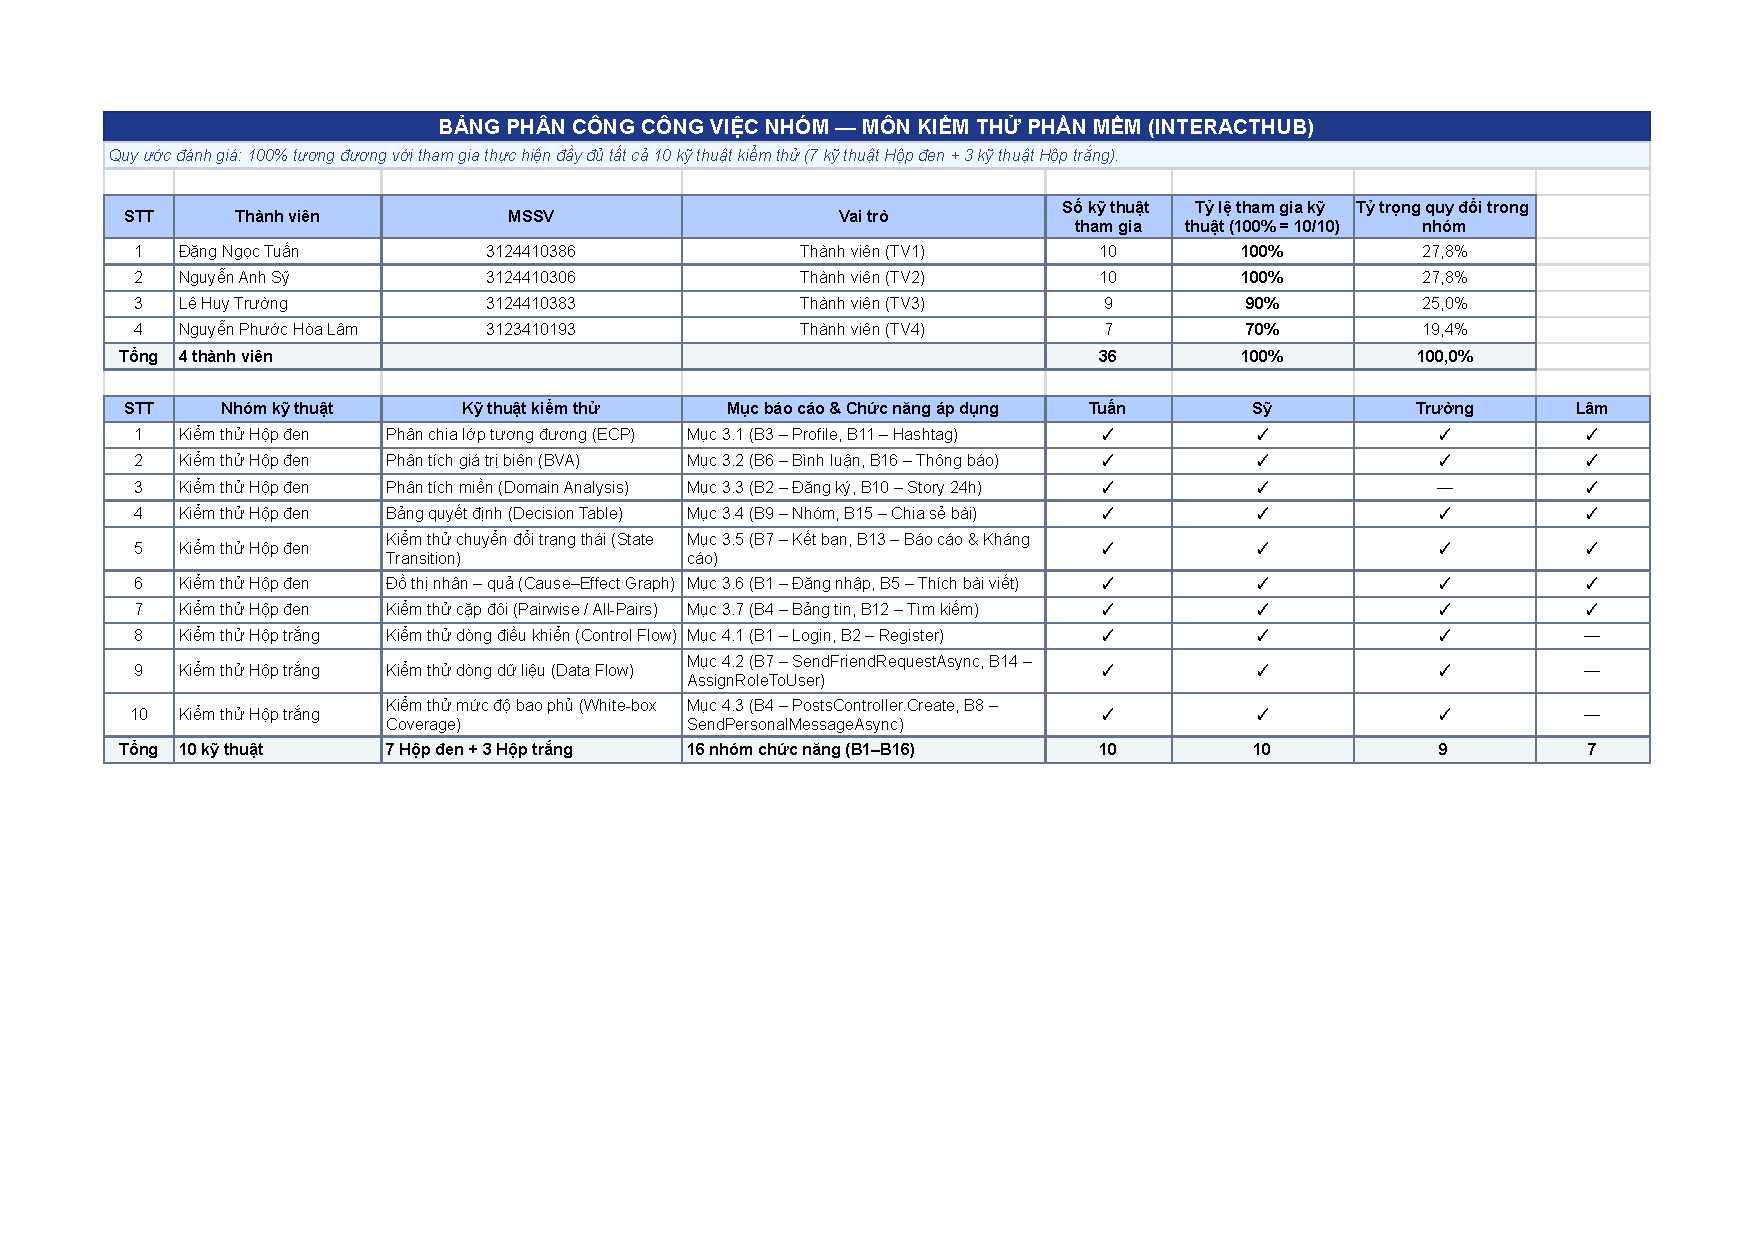
\includepdf[pages=1, fitpaper=true]{Phân công công việc - Kiểm thử phần mềm (InteractHub) - Tổng quan phân công.pdf}

\tableofcontents
\pagebreak

% ==========================================================
% CHƯƠNG 1: TỔNG QUAN DỰ ÁN & KẾ HOẠCH KIỂM THỬ
% ==========================================================
\section{CHƯƠNG 1: TỔNG QUAN DỰ ÁN VÀ KẾ HOẠCH KIỂM THỬ (TEST PLAN)}

\subsection{Giới thiệu hệ thống cần kiểm thử (InteractHub)}
\begin{tcolorbox}[colback=boxbg, colframe=boxborder, title=\textbf{Tổng quan nền tảng InteractHub}, coltitle=darkblue, fonttitle=\bfseries]
\textbf{InteractHub} là hệ thống mạng xã hội cộng đồng trực tuyến được xây dựng theo kiến trúc Client--Server, cho phép người dùng kết nối, chia sẻ nội dung, tương tác thời gian thực và quản trị cộng đồng.
\end{tcolorbox}

\begin{itemize}[leftmargin=1.2cm, noitemsep]
    \item[\textbf{--}] \textbf{Kiến trúc giao tiếp:} Kết hợp RESTful API (xác thực JWT Bearer Token, kiểm tra dữ liệu đầu vào với FluentValidation) và kênh truyền thông thời gian thực thông qua \textbf{7 SignalR Hubs}.
    \item[\textbf{--}] \textbf{Các nhóm người dùng chính:}
    \begin{itemize}[leftmargin=0.8cm, label=$\bullet$, noitemsep]
        \item \textbf{Người dùng phổ thông (User):} Đăng ký, đăng nhập, quản lý hồ sơ cá nhân, đăng bài viết, thích/bình luận/chia sẻ bài viết, kết bạn, nhắn tin 1-1 thời gian thực, tham gia nhóm cộng đồng, đăng khoảnh khắc 24h (Stories), gắn thẻ \texttt{\#hashtag}, tìm kiếm, báo cáo vi phạm, kháng cáo và nhận thông báo tức thời.
        \item \textbf{Quản trị viên (Admin):} Truy cập bảng điều khiển quản trị, xem thống kê KPI, quản lý danh sách người dùng, khóa/mở khóa tài khoản, gán/gỡ Role và xét duyệt báo cáo vi phạm cũng như yêu cầu kháng cáo bài viết.
    \end{itemize}
\end{itemize}

\subsection{Mục tiêu, phạm vi và đối tượng kiểm thử}

\subsubsection{Mục tiêu kiểm thử}
\begin{itemize}[leftmargin=1.2cm, noitemsep]
    \item[\textbf{--}] Xác minh hệ thống InteractHub hoạt động đúng theo \textbf{13 nhóm yêu cầu chức năng} (\texttt{FR-1.1} đến \texttt{FR-13.4}), \textbf{19 quy tắc nghiệp vụ} (\texttt{BR-01} đến \texttt{BR-19}) và \textbf{24 yêu cầu phi chức năng} (\texttt{NFR-1} đến \texttt{NFR-24}) từ tài liệu đặc tả SRS.
    \item[\textbf{--}] Phát hiện sớm các khiếm khuyết về logic nghiệp vụ, ràng buộc dữ liệu đầu vào, luồng chuyển đổi trạng thái, phân quyền bảo mật và xử lý ngoại lệ trên cả Frontend lẫn Backend.
    \item[\textbf{--}] Áp dụng đồng bộ các kỹ thuật kiểm thử hộp đen, hộp trắng, dựa trên yêu cầu chức năng và phi chức năng nhằm tối đa hóa độ bao phủ yêu cầu và mã nguồn.
\end{itemize}

\subsubsection{Phạm vi và danh sách 16 nhóm chức năng nghiệp vụ (B1--B16)}
Phạm vi kiểm thử bao gồm toàn bộ \textbf{16 nhóm chức năng nghiệp vụ (\texttt{B1}--\texttt{B16})} được tổng hợp trong bảng dưới đây:

\begin{longtable}{|C{1.1cm}|L{4.3cm}|L{8.4cm}|C{2.0cm}|}
\hline
\rowcolor[RGB]{179, 205, 255}
\textbf{Mã} & \textbf{Tên chức năng} & \textbf{Mô tả phạm vi chính} & \textbf{Tác nhân} \tabularnewline
\hline
\endfirsthead
\hline
\rowcolor[RGB]{179, 205, 255}
\textbf{Mã} & \textbf{Tên chức năng} & \textbf{Mô tả phạm vi chính} & \textbf{Tác nhân} \tabularnewline
\hline
\endhead
\hline
\endfoot
\textbf{B1} & Đăng nhập người dùng & Xác thực Email/Username, mật khẩu, cấp JWT, chặn tài khoản bị khóa. & User, Admin \\ \hline
\textbf{B2} & Đăng ký tài khoản & Tạo tài khoản mới, kiểm tra định dạng và ràng buộc mật khẩu. & Guest \\ \hline
\textbf{B3} & Thông tin cá nhân (Profile) & Xem, cập nhật \texttt{FullName} (2--100 ký tự), \texttt{Bio}, tải lên ảnh đại diện ($\le 5$MB, JPEG/PNG/GIF/WebP), đăng xuất. & User \\ \hline
\textbf{B4} & Bảng tin \& Bài viết & Xem bảng tin phân trang ($\le 100$), đăng bài (1--5000 ký tự + ảnh $\le 5$MB), xóa bài, đồng bộ SignalR. & User, Admin \\ \hline
\textbf{B5} & Thích bài viết (Like/Unlike) & Thích/bỏ thích bài viết và bình luận, cập nhật SignalR, không tự thông báo cho chính mình. & User \\ \hline
\textbf{B6} & Bình luận (Comments \& Replies) & Thêm bình luận/phản hồi (1--500 ký tự), sửa/xóa bình luận chính chủ, đồng bộ SignalR. & User \\ \hline
\textbf{B7} & Kết bạn \& Mạng lưới kết nối & Tìm kiếm, gửi/chấp nhận/từ chối/thu hồi lời mời, hủy kết bạn; chặn gửi trùng, tự gửi hoặc tài khoản khóa. & User \\ \hline
\textbf{B8} & Nhắn tin tức thời 1-1 & Gửi tin nhắn văn bản ($\le 2000$ ký tự) + ảnh ($\le 5$MB), múi giờ UTC+7, SignalR, xác nhận đã đọc. & User \\ \hline
\textbf{B9} & Nhóm cộng đồng (Groups) & Tạo nhóm, tham gia/rời nhóm, kiểm tra tư cách thành viên, đăng bài trong nhóm (1--5000 ký tự + ảnh $\le 5$MB). & User \\ \hline
\textbf{B10} & Khoảnh khắc 24h (Stories) & Đăng văn bản ($\le 500$ ký tự) và/hoặc ảnh ($\le 5$MB), tồn tại 24 giờ, chỉ bạn bè/tác giả xem, xóa trước 24h. & User \\ \hline
\textbf{B11} & Hashtag \& Phân loại nội dung & Tự động nhận diện \texttt{\#hashtag}, liên kết lọc bài viết và tìm kiếm theo hashtag. & User \\ \hline
\textbf{B12} & Tìm kiếm toàn hệ thống & Tìm người dùng ($\le 50$ kết quả, debounce 300ms), bài viết bảng tin, nhóm, bài trong nhóm, hội thoại. & User \\ \hline
\textbf{B13} & Báo cáo vi phạm \& Kháng cáo & Báo cáo bài viết (chi tiết 10--500 ký tự, chống trùng \texttt{Pending}), Admin duyệt/bác bỏ, User kháng cáo (10--1000 ký tự, tối đa 1 lần). & User, Admin \\ \hline
\textbf{B14} & Quản trị \& Quản lý người dùng & Phân quyền RBAC Admin, thống kê KPI, lọc/phân trang user, khóa/mở khóa tài khoản, gán/gỡ Role. & Admin \\ \hline
\textbf{B15} & Chia sẻ bài viết (Share Post) & Chia sẻ kèm chú thích (0--1000 ký tự), đóng khung bài gốc, xử lý bài gốc bị xóa, thông báo tác giả gốc. & User \\ \hline
\textbf{B16} & Thông báo & Nhận thông báo SignalR ($<1$s), bộ đếm \texttt{0--99+}, thời gian tương đối, đánh dấu đã đọc. & User \\ \hline
\end{longtable}

\subsection{Môi trường và công cụ kiểm thử}
\begin{table}[H]
\centering
\small
\begin{tabularx}{\textwidth}{|L{4.2cm}|X|}
\hline
\rowcolor[RGB]{179, 205, 255}
\textbf{Thành phần} & \textbf{Thông số kỹ thuật / Công cụ sử dụng} \tabularnewline
\hline
\textbf{Backend} & .NET 9 Web API; thư viện chính: \texttt{FluentValidation 9.0.0}, \texttt{JwtBearer 9.0.0}, \texttt{Entity Framework Core Design 9.0.0}, \texttt{Swashbuckle 6.4.6} \\ \hline
\textbf{Frontend} & \texttt{React 19.2.5}, \texttt{Vite 8.0.8}, \texttt{react-router-dom 7.14.1}, \texttt{@microsoft/signalr 8.0.17} \\ \hline
\textbf{Cơ sở dữ liệu} & MySQL, Entity Framework Core \\ \hline
\textbf{Trình duyệt kiểm thử} & Google Chrome, Microsoft Edge (phiên bản ổn định mới nhất) \\ \hline
\textbf{Công cụ kiểm thử API} & Swagger UI (\texttt{Swashbuckle}), Postman / HTTP Client \\ \hline
\textbf{Công cụ quản lý \& phân tích} & Bộ khung Unit Test (.NET), công cụ đo độ phủ mã nguồn, bảng tính theo dõi Test Case \& Defect Report \\ \hline
\end{tabularx}
\end{table}

\subsection{Tiêu chí bắt đầu và tiêu chí kết thúc}

\subsubsection{Tiêu chí bắt đầu (Entry Criteria)}
\begin{itemize}[leftmargin=1.2cm, noitemsep]
    \item[\textbf{--}] Tài liệu đặc tả yêu cầu (FinalSRS v1.0) và danh sách yêu cầu nghiệp vụ (\texttt{B1}--\texttt{B16}) đã được phê duyệt.
    \item[\textbf{--}] Mã nguồn Backend và Frontend biên dịch thành công, khởi chạy ổn định trên môi trường kiểm thử cục bộ.
    \item[\textbf{--}] Dữ liệu mẫu (tài khoản User, Admin, bài viết, nhóm mẫu) đã được khởi tạo sẵn sàng.
    \item[\textbf{--}] Tài liệu thiết kế ca kiểm thử (Test Scenarios, Test Cases) cho từng kỹ thuật đã được chuẩn bị.
\end{itemize}

\subsubsection{Tiêu chí kết thúc (Exit Criteria)}
\begin{itemize}[leftmargin=1.2cm, noitemsep]
    \item[\textbf{--}] 100\% yêu cầu nghiệp vụ từ \texttt{B1} đến \texttt{B16} được ánh xạ và kiểm thử qua ma trận truy xuất (RTM).
    \item[\textbf{--}] 100\% tổng số ca kiểm thử hộp đen và hộp trắng đã thiết kế đều được thực thi.
    \item[\textbf{--}] Không còn lỗi mức độ nghiêm trọng cao (\texttt{Critical / High}) ở trạng thái mở chưa được xử lý.
    \item[\textbf{--}] Đạt mục tiêu bao phủ hộp trắng đã đặt ra tại Mục 1.6.2 cho các hàm trọng tâm (\texttt{B4, B8}).
    \item[\textbf{--}] Báo cáo tổng hợp kết quả kiểm thử và danh sách lỗi (Defect Report) được hoàn thiện và nghiệm thu.
\end{itemize}

\subsection{Quản lý rủi ro kiểm thử}
\begin{table}[H]
\centering
\small
\begin{tabularx}{\textwidth}{|L{4.5cm}|C{2.4cm}|X|}
\hline
\rowcolor[RGB]{179, 205, 255}
\textbf{Rủi ro} & \textbf{Mức độ} & \textbf{Biện pháp giảm thiểu} \tabularnewline
\hline
Thay đổi yêu cầu hoặc giao diện trong quá trình kiểm thử & Trung bình & Cập nhật kịp thời TRD và RTM; thực hiện kiểm thử hồi quy sau mỗi lần cập nhật mã nguồn. \\ \hline
Sai lệch dữ liệu khi kiểm thử đồng thời các kết nối SignalR thời gian thực & Cao & Thiết lập kịch bản kiểm thử đa phiên trình duyệt tách biệt (User A, User B, Admin) và ghi log mốc thời gian. \\ \hline
Thiếu sót các trường hợp biên hoặc tổ hợp điều kiện phức tạp & Cao & Kết hợp chặt chẽ các kỹ thuật BVA, Domain Analysis, Decision Table và Pairwise theo bảng phân bổ. \\ \hline
Giới hạn thời gian thực thi toàn bộ ca kiểm thử hồi quy & Trung bình & Ưu tiên các ca kiểm thử thuộc luồng nghiệp vụ lõi (\texttt{B1, B2, B4, B7, B8, B13, B14}) và tự động hóa Unit Test. \\ \hline
\end{tabularx}
\end{table}

\subsection{Bảng phân bổ các kỹ thuật kiểm thử cho từng chức năng}
Nhằm đảm bảo tất cả \textbf{16 nhóm chức năng (\texttt{B1}--\texttt{B16})} đều được kiểm thử đầy đủ và mỗi kỹ thuật trọng tâm đều được áp dụng trên ít nhất \textbf{2 chức năng phù hợp nhất}, nhóm thực hiện phân bổ theo hai nhóm kỹ thuật dưới đây:

\subsubsection{Kỹ thuật kiểm thử hộp đen (Black-box Testing)}
\begin{table}[H]
\centering
\small
\begin{tabularx}{\textwidth}{|C{1.0cm}|L{4.8cm}|C{2.0cm}|X|}
\hline
\rowcolor[RGB]{179, 205, 255}
\textbf{STT} & \textbf{Kỹ thuật kiểm thử} & \textbf{Chức năng} & \textbf{Trọng tâm áp dụng} \tabularnewline
\hline
1 & Phân hoạch lớp tương đương (ECP) & \textbf{B3, B11} & Phân lớp hợp lệ/không hợp lệ của thông tin Profile, định dạng ảnh avatar và cú pháp \texttt{\#hashtag}. \\ \hline
2 & Phân tích giá trị biên (BVA) & \textbf{B6, B16} & Kiểm tra biên độ dài bình luận (1--500 ký tự), badge thông báo (\texttt{0--99+}) và độ trễ $<1$s. \\ \hline
3 & Phân tích miền (Domain Analysis) & \textbf{B2, B10} & Ràng buộc liên biến mật khẩu ($8 \le x \le 100, y=x$) và thời gian tồn tại Story ($0 \le x < 24$). \\ \hline
4 & Bảng quyết định (Decision Table) & \textbf{B9, B15} & Tổ hợp điều kiện tư cách thành viên nhóm và điều kiện chia sẻ bài viết/gửi thông báo. \\ \hline
5 & Chuyển đổi trạng thái (State Transition) & \textbf{B7, B13} & Vòng đời quan hệ kết bạn và vòng đời xử lý báo cáo vi phạm / kháng cáo bài viết. \\ \hline
6 & Đồ thị nhân -- quả (Cause--Effect Graph) & \textbf{B1, B5} & Tổ hợp điều kiện xác thực đăng nhập và logic thích/bỏ thích kèm quy tắc không tự thông báo. \\ \hline
7 & Kiểm thử cặp đôi (Pairwise Testing) & \textbf{B4, B12} & Giảm tổ hợp tham số đăng/xem bảng tin và tổ hợp tiêu chí tìm kiếm toàn hệ thống. \\ \hline
\end{tabularx}
\end{table}

\subsubsection{Kỹ thuật kiểm thử hộp trắng (White-box Testing)}
\begin{table}[H]
\centering
\small
\begin{tabularx}{\textwidth}{|C{1.0cm}|L{4.8cm}|C{2.0cm}|X|}
\hline
\rowcolor[RGB]{179, 205, 255}
\textbf{STT} & \textbf{Kỹ thuật kiểm thử} & \textbf{Chức năng} & \textbf{Trọng tâm áp dụng} \tabularnewline
\hline
1 & Kiểm thử dòng điều khiển (Control Flow) & \textbf{B1, B2} & Phủ đường đi độc lập theo độ phức tạp Cyclomatic trên \texttt{Login} và \texttt{Register}. \\ \hline
2 & Kiểm thử dòng dữ liệu (Data Flow) & \textbf{B7, B14} & Theo dõi cặp \texttt{def--use} trên \texttt{SendFriendRequestAsync} và \texttt{AssignRoleToUser}. \\ \hline
3 & Kiểm thử mức độ bao phủ (White-box Coverage) & \textbf{B4, B8} & Đo lường Statement, Branch, Condition và Path Coverage trên \texttt{PostsController.Create} và \texttt{SendPersonalMessageAsync}: \texttt{B4} đạt 100\% cả 4 tiêu chí; \texttt{B8} đạt 100\% Statement, Branch (4 nút \texttt{if}) và Path Coverage trên 5 đường cơ bản đã xác định, Condition Coverage chưa đạt 100\%. \\ \hline
\end{tabularx}
\end{table}

\pagebreak
\section{CHƯƠNG 2: ĐẶC TẢ YÊU CẦU KIỂM THỬ \& MA TRẬN TRUY XUẤT}

\subsection{Tài liệu yêu cầu kiểm thử (TRD -- Test Requirement Document)}
Từ tài liệu đặc tả yêu cầu phần mềm SRS v1.0, hệ thống \textbf{InteractHub} được chia thành \textbf{20 nhóm yêu cầu kiểm thử \texttt{T01}--\texttt{T183}} tương ứng với 16 nhóm chức năng nghiệp vụ \texttt{B1}--\texttt{B16}.
\textit{Lưu ý đối chiếu mã: tại danh mục TRD dưới đây, Đăng nhập \texttt{B1} mang mã \texttt{T01}--\texttt{T10} và Đăng ký \texttt{B2} mang mã \texttt{T11}--\texttt{T33}. Toàn bộ cột \texttt{TR\#} trong các bảng Test Cases ở Chương 3 và Chương 4 của báo cáo đều được chuẩn hóa thống nhất theo danh mục \texttt{T01}--\texttt{T183} (cùng 5 mã phụ \texttt{T27.1, T66.1, T106.1, T114.1, T167.1}) tại Mục 2.1 này; cột ``Mã ở RTM'' trong Bảng tổng hợp Mục 2.3 chỉ dùng để đối chiếu chéo với bảng tính gốc của dự án (nơi \texttt{B2} đánh trước \texttt{T01}--\texttt{T23} và \texttt{B1} là \texttt{T24}--\texttt{T33}).}

\noindent\textbf{1. Đăng nhập người dùng -- B1}
\begin{itemize}[leftmargin=0.9cm, label=$\bullet$, itemsep=2pt, topsep=4pt]
    \item \textbf{T01} Tên đăng nhập không được để trống.
    \item \textbf{T02} Mật khẩu không được để trống.
    \item \textbf{T03} Tài khoản phải đã được đăng ký trước đó trong hệ thống.
    \item \textbf{T04} Mật khẩu nhập vào phải trùng khớp với mật khẩu đã đăng ký.
    \item \textbf{T05} Tài khoản Quản trị viên không được phép đăng nhập ở trang dành cho người dùng thường mà phải dùng trang đăng nhập riêng của Quản trị viên.
    \item \textbf{T06} Khi nhập đúng thông tin, hệ thống cho phép đăng nhập thành công và duy trì phiên làm việc trong 60 phút.
    \item \textbf{T07} Nếu sai tên đăng nhập hoặc mật khẩu, hệ thống từ chối đăng nhập và hiện thông báo chung ``Sai tên đăng nhập hoặc mật khẩu'', không chỉ rõ sai mục nào để đảm bảo an toàn.
    \item \textbf{T08} Hệ thống hiện không giới hạn số lần nhập sai mật khẩu.
    \item \textbf{T09} Sau khi đăng nhập thành công, trình duyệt tự động ghi nhớ trạng thái đăng nhập để người dùng không phải đăng nhập lại khi chuyển trang.
    \item \textbf{T10} Ngay khi đăng nhập thành công, toàn bộ giao diện đang mở tự động cập nhật sang trạng thái đã đăng nhập.
\end{itemize}
\smallskip
\noindent\textbf{2. Đăng ký tài khoản -- B2}
\begin{itemize}[leftmargin=0.9cm, label=$\bullet$, itemsep=2pt, topsep=4pt]
    \item \textbf{T11} Tên đăng nhập không được để trống.
    \item \textbf{T12} Tên đăng nhập phải có ít nhất 3 ký tự.
    \item \textbf{T13} Tên đăng nhập không được vượt quá 20 ký tự.
    \item \textbf{T14} Tên đăng nhập chỉ được chứa chữ cái không dấu a--z, A--Z, chữ số 0--9 và dấu gạch dưới \texttt{\_}.
    \item \textbf{T15} Tên đăng nhập chưa từng được người khác sử dụng, không được trùng.
    \item \textbf{T16} Email không được để trống.
    \item \textbf{T17} Email phải đúng định dạng hợp lệ.
    \item \textbf{T18} Email chưa từng được đăng ký cho tài khoản khác, không được trùng.
    \item \textbf{T19} Họ và tên không được để trống.
    \item \textbf{T20} Họ và tên phải có ít nhất 2 ký tự, không tính khoảng trắng thừa ở đầu và cuối.
    \item \textbf{T21} Họ và tên không được vượt quá 100 ký tự.
    \item \textbf{T22} Mật khẩu không được để trống.
    \item \textbf{T23} Mật khẩu phải có ít nhất 8 ký tự.
    \item \textbf{T24} Mật khẩu phải có ít nhất 1 chữ cái viết hoa A--Z.
    \item \textbf{T25} Mật khẩu phải có ít nhất 1 chữ cái viết thường a--z.
    \item \textbf{T26} Mật khẩu phải có ít nhất 1 chữ số 0--9.
    \item \textbf{T27} Mật khẩu phải có ít nhất 1 ký tự đặc biệt.
    \item \textbf{T27.1} Mật khẩu xác nhận phải có độ dài bằng và nội dung trùng khớp hoàn toàn với Mật khẩu; nếu không khớp, hệ thống từ chối và báo lỗi tại ô xác nhận.
    \item \textbf{T28} Mật khẩu được chấm điểm độ mạnh từ 0 đến 100 và hiển thị cảnh báo nếu chưa đạt.
    \item \textbf{T29} Mật khẩu phải được mã hóa an toàn trước khi lưu trữ, tuyệt đối không lưu dạng chữ thông thường.
    \item \textbf{T30} Khi mọi thông tin hợp lệ, hệ thống tạo tài khoản mới và mặc định cấp quyền Người dùng.
    \item \textbf{T31} Nếu quá trình cấp quyền mặc định gặp lỗi, hệ thống phải hủy bỏ tài khoản vừa tạo ngay lập tức và báo lỗi đăng ký thất bại.
    \item \textbf{T32} Đăng ký thành công thì thông báo cho người dùng và chuyển hướng về trang đăng nhập.
    \item \textbf{T33} Đăng ký thất bại phải hiển thị thông báo lỗi rõ ràng ngay tại từng ô nhập bị sai.
\end{itemize}
\smallskip
\noindent\textbf{3. Xem thông tin người dùng -- B3}
\begin{itemize}[leftmargin=0.9cm, label=$\bullet$, itemsep=2pt, topsep=4pt]
    \item \textbf{T34} Người dùng phải đăng nhập mới xem được thông tin hồ sơ.
    \item \textbf{T35} Nếu tìm xem tài khoản không tồn tại, hệ thống thông báo ``Không tìm thấy người dùng''.
    \item \textbf{T36} Thông tin hiển thị tuyệt đối không được để lộ dữ liệu nhạy cảm.
    \item \textbf{T37} Hồ sơ hiển thị đầy đủ các thông tin cơ bản: Mã tài khoản, Tên đăng nhập, Email, Họ tên, Ảnh đại diện và Tiểu sử.
\end{itemize}
\smallskip
\noindent\textbf{4. Cập nhật hồ sơ cá nhân -- B3}
\begin{itemize}[leftmargin=0.9cm, label=$\bullet$, itemsep=2pt, topsep=4pt]
    \item \textbf{T38} Người dùng phải đăng nhập mới sửa được hồ sơ.
    \item \textbf{T39} Chỉ chủ tài khoản mới có quyền chỉnh sửa hồ sơ của chính mình.
    \item \textbf{T40} Nếu cố tình sửa hồ sơ của người khác, hệ thống chặn lại và báo ``Bạn không có quyền cập nhật người dùng này''.
    \item \textbf{T41} Họ và tên không được để trống khi cập nhật.
    \item \textbf{T42} Họ và tên phải có ít nhất 2 ký tự.
    \item \textbf{T43} Họ và tên không được vượt quá 100 ký tự.
    \item \textbf{T44} Phần Tiểu sử là tùy chọn, người dùng có thể bỏ trống.
    \item \textbf{T45} Ảnh đại diện là tùy chọn, có thể giữ nguyên hoặc bỏ trống.
    \item \textbf{T46} Nếu tài khoản cần cập nhật không tồn tại, hệ thống thông báo ``Không tìm thấy người dùng''.
    \item \textbf{T47} Cập nhật thành công thì lưu lại thông tin mới và thông báo cho người dùng.
    \item \textbf{T48} Ngay khi cập nhật thành công, tên hoặc thông tin mới của người dùng được đồng bộ tức thì trên màn hình của tất cả người khác đang trực tuyến.
\end{itemize}
\smallskip
\noindent\textbf{5. Tải lên ảnh đại diện -- B3}
\begin{itemize}[leftmargin=0.9cm, label=$\bullet$, itemsep=2pt, topsep=4pt]
    \item \textbf{T49} Người dùng phải đăng nhập mới đổi được ảnh đại diện.
    \item \textbf{T50} Chỉ chủ tài khoản mới được đổi ảnh đại diện của mình; người khác cố thực hiện sẽ bị từ chối.
    \item \textbf{T51} Bắt buộc phải chọn tệp ảnh trước khi tải lên; nếu chưa chọn mà bấm lưu, hệ thống báo ``Vui lòng chọn tệp để tải lên''.
    \item \textbf{T52} Dung lượng ảnh không được vượt quá 5 MB; nếu quá dung lượng, hệ thống từ chối và báo lỗi.
    \item \textbf{T53} Chỉ chấp nhận các định dạng ảnh phổ biến gồm JPEG, PNG, GIF và WebP.
    \item \textbf{T54} Nếu tải lên tệp không phải định dạng ảnh cho phép, hệ thống từ chối và báo lỗi định dạng.
    \item \textbf{T55} Trước khi gửi lên máy chủ, hệ thống tự động thu gọn kích thước ảnh xuống tối đa $256\times 256$ pixel để tải nhanh và tiết kiệm dung lượng.
    \item \textbf{T56} Nếu tài khoản không tồn tại, hệ thống thông báo ``Không tìm thấy người dùng''.
    \item \textbf{T57} Tải ảnh thành công thì cập nhật và hiển thị ngay ảnh đại diện mới.
    \item \textbf{T58} Ảnh đại diện mới cũng được cập nhật tức thì trên màn hình của những người dùng khác đang trực tuyến.
\end{itemize}
\smallskip
\noindent\textbf{6. Cơ chế xác thực \& Bảo mật phiên đăng nhập -- B1, B2, B3}
\begin{itemize}[leftmargin=0.9cm, label=$\bullet$, itemsep=2pt, topsep=4pt]
    \item \textbf{T59} Phiên đăng nhập được bảo vệ bằng mã xác thực chống giả mạo để đảm bảo an toàn tài khoản.
    \item \textbf{T60} Các thiết lập bảo mật và thời hạn phiên đăng nhập được quản lý tập trung trong cấu hình hệ thống.
    \item \textbf{T61} Mỗi phiên đăng nhập của người dùng có thời hạn mặc định là 60 phút.
    \item \textbf{T62} Mã phiên đăng nhập lưu giữ đúng thông tin nhận diện người dùng gồm Mã số, Tên đăng nhập, Email, Họ tên và Vai trò.
    \item \textbf{T63} Trình duyệt lưu giữ thông tin phiên đăng nhập và hồ sơ cơ bản để duy trì trải nghiệm xuyên suốt khi sử dụng.
\end{itemize}
\smallskip
\noindent\textbf{7. Đăng bài viết trên Bảng tin \& Xem Bảng tin -- B4}
\begin{itemize}[leftmargin=0.9cm, label=$\bullet$, itemsep=2pt, topsep=4pt]
    \item \textbf{T64} Người dùng phải đăng nhập mới có quyền đăng bài và xem Bảng tin.
    \item \textbf{T65} Không thể đăng bài viết nếu để trống nội dung hoặc chỉ gõ toàn dấu cách.
    \item \textbf{T66} Nội dung bài viết phải dài từ 1 đến tối đa 5.000 ký tự.
    \item \textbf{T66.1} Khi không đọc lại được bài viết vừa tạo sau khi lưu, hệ thống trả về HTTP 500 với thông báo ``Failed to retrieve created post'', không phát sự kiện \texttt{PostCreated} và không gửi thông báo bài viết mới.
    \item \textbf{T67} Chữ trong bài viết phải tự động xuống dòng gọn gàng, không bị tràn khung hay vỡ giao diện.
    \item \textbf{T68} Có thể đính kèm ảnh hợp lệ thuộc định dạng JPEG, PNG, GIF, WebP với dung lượng tối đa 5 MB.
    \item \textbf{T69} Hệ thống từ chối nếu ảnh đính kèm vượt quá 5 MB hoặc sai định dạng cho phép.
    \item \textbf{T70} Sau khi đăng bài thành công, ô nhập liệu tự động xóa trắng và bài viết mới xuất hiện ngay trên đầu Bảng tin.
    \item \textbf{T71} Bài viết mới tự động hiện lên Bảng tin của bạn bè ngay lập tức mà không cần tải lại trang.
    \item \textbf{T72} Bạn bè của người đăng nhận được thông báo về bài viết mới chia sẻ công khai.
    \item \textbf{T73} Bảng tin hiển thị các bài viết công khai của bản thân, bạn bè và người dùng khác, xếp bài mới nhất lên đầu.
    \item \textbf{T74} Bảng tin hỗ trợ cuộn xem tiếp các bài viết cũ hơn, tải tối đa 100 bài mỗi lần.
    \item \textbf{T75} Bảng tin chỉ hiển thị các bài viết đang hoạt động, không hiện lại bài đã bị xóa.
\end{itemize}
\smallskip
\noindent\textbf{8. Xóa bài viết \& Bảo toàn dữ liệu -- B4}
\begin{itemize}[leftmargin=0.9cm, label=$\bullet$, itemsep=2pt, topsep=4pt]
    \item \textbf{T76} Người dùng phải đăng nhập mới thực hiện được thao tác xóa bài.
    \item \textbf{T77} Chỉ tác giả bài viết mới thấy nút Xóa và có quyền xóa bài của mình.
    \item \textbf{T78} Người dùng không thể xóa bài viết của người khác vì nút xóa được ẩn đi.
    \item \textbf{T79} Khi bấm xóa, hệ thống hiện hộp thoại hỏi xác nhận để tránh xóa nhầm.
    \item \textbf{T80} Sau khi xác nhận xóa, bài viết biến mất ngay khỏi Bảng tin, trang cá nhân và nhóm mà không cần tải lại trang.
    \item \textbf{T81} Nếu xóa bài trong nhóm, các thành viên khác đang xem nhóm cũng thấy bài viết biến mất ngay lập tức.
\end{itemize}
\smallskip
\noindent\textbf{9. Thích bài viết và bỏ thích bài viết -- B5}
\begin{itemize}[leftmargin=0.9cm, label=$\bullet$, itemsep=2pt, topsep=4pt]
    \item \textbf{T82} Dưới mỗi bài viết hiển thị nút biểu tượng trái tim kèm tổng số lượt thích.
    \item \textbf{T83} Nhấn vào trái tim màu trắng thì đổi sang màu đỏ và số lượt thích tăng thêm 1.
    \item \textbf{T84} Nhấn lại vào trái tim màu đỏ thì trở về màu trắng và số lượt thích giảm đi 1.
    \item \textbf{T85} Khi có người bấm thích bài viết, người khác đang xem bài viết đó cũng thấy số lượt thích tự động cập nhật theo.
    \item \textbf{T86} Tác giả nhận được thông báo ngay khi có người thích bài viết của mình, không tự thông báo nếu tự thích bài mình.
    \item \textbf{T87} Người dùng cũng có thể nhấn thả tim cho từng bình luận bên dưới bài viết.
\end{itemize}
\smallskip
\noindent\textbf{10. Bình luận bài viết -- B6}
\begin{itemize}[leftmargin=0.9cm, label=$\bullet$, itemsep=2pt, topsep=4pt]
    \item \textbf{T88} Dưới mỗi bài viết có nút ``Bình luận''; bấm vào sẽ mở ô nhập, danh sách bình luận và số lượng bình luận.
    \item \textbf{T89} Không thể gửi bình luận nếu để trống hoặc chỉ gõ dấu cách.
    \item \textbf{T90} Có thể nhấn phím Enter hoặc bấm nút Gửi để đăng bình luận.
    \item \textbf{T91} Khi gửi thành công, bình luận mới hiện ra ngay, ô nhập được xóa trắng và số lượng bình luận tăng thêm 1.
    \item \textbf{T92} Người khác đang mở bài viết thấy bình luận mới hiện lên ngay lập tức mà không cần tải lại trang.
    \item \textbf{T93} Tác giả bài viết nhận được thông báo chuông kèm đoạn trích nội dung bình luận mới.
    \item \textbf{T94} Người viết bình luận chỉ được sửa hoặc xóa bình luận của chính mình; không thấy nút Sửa/Xóa ở bình luận của người khác.
    \item \textbf{T95} Khi bấm Xóa bình luận, hệ thống hỏi xác nhận; đồng ý xóa thì bình luận biến mất và số bình luận giảm đi 1.
\end{itemize}
\smallskip
\noindent\textbf{11. Kết bạn \& Mạng lưới kết nối -- B7}
\begin{itemize}[leftmargin=0.9cm, label=$\bullet$, itemsep=2pt, topsep=4pt]
    \item \textbf{T96} Hỗ trợ tìm kiếm người dùng theo tên hiển thị hoặc email, trả về danh sách có phân trang kèm trạng thái quan hệ hiện tại gồm chưa kết bạn, chờ duyệt hoặc đã là bạn bè.
    \item \textbf{T97} Không thể tự gửi lời mời kết bạn cho chính mình; nút kết bạn bị ẩn trên trang cá nhân của bản thân và hệ thống chặn nếu cố gửi.
    \item \textbf{T98} Không thể gửi lời mời kết bạn trùng lặp nếu hai người đang chờ xác nhận hoặc đã là bạn bè.
    \item \textbf{T99} Lời mời kết bạn mới được lưu ở trạng thái ``Chờ duyệt'' và gửi thông báo ngay lập tức cho người nhận.
    \item \textbf{T100} Người nhận có thể bấm ``Chấp nhận''; hai người trở thành bạn bè và danh sách bạn bè của cả hai được cập nhật ngay.
    \item \textbf{T101} Người nhận có thể bấm ``Từ chối'' lời mời kết bạn; lời mời sẽ bị gỡ bỏ.
    \item \textbf{T102} Người gửi có thể thu hồi hoặc hủy lời mời kết bạn khi người nhận chưa phản hồi.
    \item \textbf{T103} Người dùng có thể hủy kết bạn với bạn bè hiện tại; hai bên không còn trong danh sách bạn bè của nhau nữa.
    \item \textbf{T104} Danh sách bạn bè hiển thị rõ Tên, Ảnh đại diện, Số bạn chung, nút nhắn tin nhanh và hỗ trợ phân trang.
    \item \textbf{T105} Danh sách lời mời kết bạn hiển thị các lời mời đã nhận kèm nút ``Xác nhận'' và ``Xóa bỏ''.
    \item \textbf{T106} Không thể thực hiện kết bạn với tài khoản đang bị Quản trị viên khóa.
    \item \textbf{T106.1} Không cho phép người dùng gửi lời mời kết bạn tới tài khoản có vai trò Quản trị viên (\texttt{Admin}); phương thức \texttt{SendFriendRequestAsync} chặn thao tác và ném ngoại lệ nghiệp vụ.
\end{itemize}
\smallskip
\noindent\textbf{12. Nhắn tin tức thời 1-1 -- B8}
\begin{itemize}[leftmargin=0.9cm, label=$\bullet$, itemsep=2pt, topsep=4pt]
    \item \textbf{T107} Màn hình tin nhắn hiển thị danh sách các cuộc trò chuyện gần đây, xếp theo tin nhắn mới nhất lên đầu và hiển thị theo giờ Việt Nam UTC+7.
    \item \textbf{T108} Không được gửi tin nhắn trống hoặc chỉ có khoảng trắng nếu không đính kèm ảnh; nếu vi phạm, hệ thống chặn gửi và báo lỗi.
    \item \textbf{T109} Nội dung một tin nhắn chữ không được vượt quá 2.000 ký tự; nếu vượt quá, hệ thống báo lỗi và không cho gửi.
    \item \textbf{T110} Hỗ trợ gửi kèm ảnh định dạng JPEG, PNG, GIF, WebP với dung lượng tối đa 5 MB; ảnh sai định dạng hoặc quá nặng sẽ bị từ chối.
    \item \textbf{T111} Tin nhắn được gửi và nhận ngay lập tức theo thời gian thực giữa hai người mà không cần tải lại trang.
    \item \textbf{T112} Khi người nhận đang mở khung chat, tin nhắn mới tự động cuộn xuống cuối và tự động đánh dấu là ``Đã đọc''.
    \item \textbf{T113} Khi người nhận không mở khung chat, tin nhắn mới sẽ làm tăng số đếm tin nhắn chưa đọc trên thanh điều hướng.
    \item \textbf{T114} Không thể gửi tin nhắn đến tài khoản chưa kích hoạt, tài khoản bị khóa hoặc người đã chặn mình.
    \item \textbf{T114.1} Chặn gửi tin nhắn cá nhân ở tầng dịch vụ khi thiếu mã người nhận (\texttt{receiverId} \texttt{null} hoặc rỗng); phương thức \texttt{SendPersonalMessageAsync} ném ngoại lệ \texttt{ArgumentException}.
    \item \textbf{T115} Nếu gửi tin nhắn thất bại do mất mạng hoặc lỗi hệ thống, màn hình hiện biểu tượng cảnh báo lỗi kèm nút ``Thử lại''.
\end{itemize}
\smallskip
\noindent\textbf{13. Đăng bài viết trong Nhóm -- B9}
\begin{itemize}[leftmargin=0.9cm, label=$\bullet$, itemsep=2pt, topsep=4pt]
    \item \textbf{T116} Người dùng phải đăng nhập mới truy cập và đăng bài trong nhóm được.
    \item \textbf{T117} Chỉ thành viên chính thức của nhóm mới được phép đăng bài vào nhóm đó.
    \item \textbf{T118} Người chưa tham gia nhóm sẽ không thấy nút đăng bài hoặc bị chặn thao tác đăng.
    \item \textbf{T119} Nội dung bài viết trong nhóm không được để trống, dài từ 1 đến 5.000 ký tự.
    \item \textbf{T120} Cho phép đính kèm ảnh hợp lệ định dạng JPEG, PNG, GIF, WebP với dung lượng tối đa 5 MB khi đăng bài trong nhóm.
    \item \textbf{T121} Đăng bài thành công thì bài viết hiện ngay trên đầu trang nhóm.
    \item \textbf{T122} Các thành viên khác đang mở trang nhóm sẽ thấy bài viết mới hiện lên ngay lập tức.
    \item \textbf{T123} Bài viết đăng trong nhóm chỉ hiển thị bên trong nhóm, không hiện lẫn ra Bảng tin chung bên ngoài.
\end{itemize}
\smallskip
\noindent\textbf{14. Tin ngắn 24h -- B10}
\begin{itemize}[leftmargin=0.9cm, label=$\bullet$, itemsep=2pt, topsep=4pt]
    \item \textbf{T124} Người dùng phải đăng nhập mới tạo, xem và xóa được Story.
    \item \textbf{T125} Story bắt buộc phải có ít nhất hình ảnh hoặc chữ, không được bỏ trống cả hai.
    \item \textbf{T126} Nội dung chữ trên Story tối đa 500 ký tự.
    \item \textbf{T127} Chữ trên Story phải tự động xuống dòng gọn gàng, không tràn ra ngoài khung hiển thị.
    \item \textbf{T128} Ảnh đăng Story phải đúng định dạng cho phép JPEG, PNG, WebP, GIF và dung lượng không quá 5 MB.
    \item \textbf{T129} Đăng Story thành công thì hiện ngay trên thanh Khoảnh khắc của bản thân và bạn bè.
    \item \textbf{T130} Người dùng chỉ xem được Story của chính mình và của bạn bè đã kết nối.
    \item \textbf{T131} Người lạ chưa kết bạn không thể xem Story của nhau.
    \item \textbf{T132} Story tự động tồn tại trong đúng 24 giờ kể từ lúc đăng, sau đó tự biến mất khỏi danh sách.
    \item \textbf{T133} Tác giả có thể chủ động xóa Story của mình bất kỳ lúc nào trước khi hết 24 giờ.
    \item \textbf{T134} Sau khi xóa, Story biến mất ngay lập tức trên màn hình của bản thân và bạn bè.
\end{itemize}
\smallskip
\noindent\textbf{15. Thẻ chủ đề \& Tìm kiếm Hashtag -- B11}
\begin{itemize}[leftmargin=0.9cm, label=$\bullet$, itemsep=2pt, topsep=4pt]
    \item \textbf{T135} Khi bài viết có từ khóa bắt đầu bằng dấu \texttt{\#}, hệ thống tự động nhận diện là thẻ chủ đề.
    \item \textbf{T136} Hashtag trong bài viết hiển thị nổi bật bằng màu xanh và có thể bấm vào được.
    \item \textbf{T137} Khi bấm vào một hashtag, hệ thống tự động lọc và hiển thị toàn bộ bài viết có gắn hashtag đó.
    \item \textbf{T138} Người dùng có thể gõ từ khóa bắt đầu bằng \texttt{\#} vào thanh tìm kiếm để tìm bài viết liên quan.
    \item \textbf{T139} Nếu hashtag có bài viết, hệ thống trả về danh sách các bài viết tương ứng.
    \item \textbf{T140} Nếu hashtag chưa có bài viết nào, hệ thống thông báo ``Không tìm thấy bài viết nào phù hợp''.
    \item \textbf{T141} Giao diện có nút Quay lại hoặc Xóa bộ lọc để người dùng dễ dàng trở về Bảng tin bình thường.
\end{itemize}
\smallskip
\noindent\textbf{16. Tìm kiếm toàn hệ thống -- B12}
\begin{itemize}[leftmargin=0.9cm, label=$\bullet$, itemsep=2pt, topsep=4pt]
    \item \textbf{T142} Thanh tìm kiếm chung hỗ trợ tìm người dùng theo Họ tên hoặc Tên đăng nhập, có phân trang và hiện trạng thái kết bạn.
    \item \textbf{T143} Thanh tìm kiếm hỗ trợ tìm bài viết trên Bảng tin theo nội dung bài hoặc tên tác giả.
    \item \textbf{T144} Trang danh sách Nhóm có ô tìm kiếm theo tên nhóm, tự động lọc kết quả ngay khi đang gõ.
    \item \textbf{T145} Bên trong từng Nhóm có ô tìm kiếm nhanh bài viết theo nội dung hoặc tên người đăng trong nhóm đó.
    \item \textbf{T146} Trang Tin nhắn có ô tìm kiếm giúp lọc nhanh cuộc trò chuyện theo tên bạn bè hoặc tên nhóm chat.
\end{itemize}
\smallskip
\noindent\textbf{17. Báo cáo vi phạm \& Kháng cáo bài viết -- B13}
\begin{itemize}[leftmargin=0.9cm, label=$\bullet$, itemsep=2pt, topsep=4pt]
    \item \textbf{T147} Người dùng đã đăng nhập có quyền báo cáo bài viết vi phạm; bắt buộc chọn lý do gồm Spam, Quấy rối, Không phù hợp, Bạo lực, Bản quyền hoặc Khác, đồng thời nhập mô tả từ 10--500 ký tự.
    \item \textbf{T148} Mỗi người chỉ được báo cáo một bài viết tối đa 1 lần trong khi chờ xử lý; nếu gửi trùng, hệ thống từ chối và báo ``Bạn đã báo cáo bài viết này rồi''.
    \item \textbf{T149} Báo cáo mới gửi sẽ ở trạng thái ``Đang chờ xử lý'' và hiện ngay trong danh sách kiểm duyệt của Quản trị viên.
    \item \textbf{T150} Quản trị viên có trang riêng xem toàn bộ bài viết bị báo cáo và lọc được theo trạng thái: Chờ xử lý, Đã giải quyết, Đã bác bỏ, Đang kháng cáo.
    \item \textbf{T151} Giao diện kiểm duyệt hiển thị đầy đủ bài viết bị báo cáo gồm chữ, ảnh và tác giả, cùng thông tin người báo cáo, thời gian và lý do.
    \item \textbf{T152} Khi Quản trị viên chọn ``Gỡ bỏ bài viết'': bài viết bị ẩn khỏi Bảng tin công khai và hệ thống gửi thông báo cho tác giả biết.
    \item \textbf{T153} Khi Quản trị viên chọn ``Bác bỏ báo cáo'': bài viết vẫn giữ nguyên trên Bảng tin và báo cáo chuyển sang trạng thái ``Đã bác bỏ''.
    \item \textbf{T154} Tác giả có bài bị gỡ sẽ nhìn thấy thông báo nêu rõ lý do và nút ``Kháng cáo''.
    \item \textbf{T155} Người dùng gửi kháng cáo bằng cách nhập lý do giải trình từ 10--1.000 ký tự; trạng thái chuyển sang ``Đang kháng cáo''.
    \item \textbf{T156} Đơn đang kháng cáo được đánh dấu nổi bật bằng nhãn cảnh báo để Quản trị viên dễ nhận biết và đọc toàn bộ lời giải trình.
    \item \textbf{T157} Nếu Quản trị viên ``Chấp thuận kháng cáo'': bài viết được khôi phục lại công khai và gửi thông báo kết quả cho tác giả.
    \item \textbf{T158} Nếu Quản trị viên ``Từ chối kháng cáo'': bài viết tiếp tục bị gỡ, gửi thông báo quyết định cuối cùng cho tác giả; mỗi bài chỉ được kháng cáo tối đa 1 lần.
\end{itemize}
\smallskip
\noindent\textbf{18. Bảng điều khiển Quản trị \& Quản lý Người dùng -- B14}
\begin{itemize}[leftmargin=0.9cm, label=$\bullet$, itemsep=2pt, topsep=4pt]
    \item \textbf{T159} Chỉ tài khoản có quyền Quản trị viên mới đăng nhập được vào cổng quản trị và mở trang quản trị; tài khoản thường truy cập trái phép sẽ bị chặn.
    \item \textbf{T160} Trang tổng quan Quản trị hiển thị các con số thống kê chính: Tổng số người dùng, Tổng số bài viết, Số báo cáo chờ xử lý và Số tài khoản đang bị khóa.
    \item \textbf{T161} Quản trị viên xem được danh sách toàn bộ người dùng theo từng trang 10, 20 hoặc 50 người với đầy đủ: Ảnh đại diện, Tên tài khoản, Email, Vai trò, Ngày đăng ký, Trạng thái.
    \item \textbf{T162} Hỗ trợ tìm nhanh tài khoản trong danh sách quản trị theo Tên người dùng hoặc Email.
    \item \textbf{T163} Hỗ trợ lọc danh sách người dùng theo Trạng thái gồm Tất cả, Đang hoạt động, Đang bị khóa và theo Vai trò gồm Tất cả, Quản trị viên, Người dùng.
    \item \textbf{T164} Quản trị viên có quyền ``Khóa tài khoản'' đối với người vi phạm; hệ thống yêu cầu nhập lý do và xác nhận trước khi khóa.
    \item \textbf{T165} Quản trị viên không được phép tự khóa tài khoản của chính mình và không được khóa tài khoản Quản trị viên cấp cao hơn.
    \item \textbf{T166} Ngay khi một tài khoản bị khóa, phiên đăng nhập hiện tại của người đó bị ngắt lập tức; nếu đang dùng sẽ bị đẩy ra màn hình đăng nhập kèm thông báo tài khoản đã bị khóa.
    \item \textbf{T167} Quản trị viên có quyền ``Mở khóa tài khoản'' để khôi phục lại quyền truy cập cho người dùng.
    \item \textbf{T167.1} Quản trị viên có quyền gán vai trò cho người dùng (\texttt{POST /api/admin/assign-role}); hệ thống kiểm tra tài khoản tồn tại, vai trò hợp lệ, chặn gán trùng vai trò đã có và ghi nhận thay đổi quyền trong cơ sở dữ liệu.
\end{itemize}
\smallskip
\noindent\textbf{19. Chia sẻ bài viết -- B15}
\begin{itemize}[leftmargin=0.9cm, label=$\bullet$, itemsep=2pt, topsep=4pt]
    \item \textbf{T168} Dưới mỗi bài viết có nút ``Chia sẻ''; bấm vào sẽ mở hộp thoại tùy chọn chia sẻ.
    \item \textbf{T169} Người dùng có thể viết thêm lời dẫn từ 0--1.000 ký tự hoặc bỏ trống lời dẫn vẫn chia sẻ được.
    \item \textbf{T170} Bấm ``Chia sẻ ngay'' thì bài chia sẻ xuất hiện ngay trên đầu Bảng tin của người dùng.
    \item \textbf{T171} Bài chia sẻ ghi rõ dòng chữ ``Bài viết được chia sẻ'', tên người chia sẻ và đóng khung bài viết gốc bên trong.
    \item \textbf{T172} Bấm vào phần khung bài viết gốc sẽ mở ra trang xem chi tiết bài gốc đó.
    \item \textbf{T173} Tác giả bài gốc nhận được thông báo khi có người chia sẻ bài viết của mình.
    \item \textbf{T174} Nếu bài viết gốc đã bị tác giả xóa, nội dung bài gốc sẽ không còn hiển thị trong các bài đã chia sẻ lại nó.
\end{itemize}
\smallskip
\noindent\textbf{20. Thông báo và mở bài viết từ thông báo -- B16}
\begin{itemize}[leftmargin=0.9cm, label=$\bullet$, itemsep=2pt, topsep=4pt]
    \item \textbf{T175} Biểu tượng chuông trên thanh điều hướng tự động hiện chấm đỏ và số lượng khi có người tương tác bài viết của mình.
    \item \textbf{T176} Bấm vào biểu tượng chuông sẽ mở danh sách thông báo xếp từ mới nhất xuống cũ hơn.
    \item \textbf{T177} Thông báo vừa phát sinh dưới 1 phút hiển thị thời gian là ``vừa xong''.
    \item \textbf{T178} Thông báo từ 1 phút đến dưới 60 phút hiển thị dạng ``\{số\} phút trước''.
    \item \textbf{T179} Thông báo từ 1 giờ đến dưới 24 giờ hiển thị dạng ``\{số\} giờ trước''; trong tài liệu gốc mục này từng in nhầm nhãn T178 lần 2, trong bảng Test Case và RTM đánh mã là T179.
    \item \textbf{T180} Khi di chuột vào dòng thông báo, con trỏ đổi thành hình bàn tay và dòng thông báo sáng lên để nhận biết có thể bấm vào.
    \item \textbf{T181} Bấm vào dòng thông báo sẽ tự động đánh dấu ``Đã đọc'' và mở sang trang chi tiết bài viết.
    \item \textbf{T182} Trang chi tiết hiển thị đầy đủ nội dung, ảnh lớn, số lượt thích và danh sách bình luận của bài viết đó.
    \item \textbf{T183} Nếu bài viết đó đã bị xóa trước khi người dùng bấm vào thông báo, màn hình thông báo rõ ``Bài viết không tồn tại'' thay vì bị lỗi đứng trang.
\end{itemize}
\smallskip

\subsection{Danh sách kịch bản kiểm thử (Test Scenarios)}
Từ 183 yêu cầu kỹ thuật trong TRD, nhóm kiểm thử xây dựng \textbf{58 kịch bản kiểm thử (\texttt{TS01}--\texttt{TS58})} bao quát đầy đủ các luồng kiểm tra hợp lệ (Positive), kiểm tra ràng buộc/ngoại lệ (Negative/Validation), phân quyền bảo mật (Security) và đồng bộ thời gian thực (Realtime). Bảng dưới đây tổng hợp toàn bộ 58 kịch bản theo từng nhóm chức năng:

\begin{longtable}{|C{1.3cm}|C{1.2cm}|L{4.8cm}|L{8.5cm}|}
\hline
\rowcolor[RGB]{179, 205, 255}
\textbf{Mã TS} & \textbf{BRD} & \textbf{Tên kịch bản} & \textbf{Phạm vi kiểm tra chính} \tabularnewline
\hline
\endfirsthead
\hline
\rowcolor[RGB]{179, 205, 255}
\textbf{Mã TS} & \textbf{BRD} & \textbf{Tên kịch bản} & \textbf{Phạm vi kiểm tra chính} \tabularnewline
\hline
\endhead
\hline
\endfoot
TS01 & B1 & Validate đăng nhập & Bỏ trống UserName/Password, tài khoản không tồn tại, sai mật khẩu. \\ \hline
TS02 & B1 & Functional -- Đăng nhập thành công & Đăng nhập đúng tài khoản User, lưu JWT Token, nút ẩn/hiện mật khẩu. \\ \hline
TS03 & B1 & Security -- Phân quyền đăng nhập & Chặn Admin đăng nhập cổng User; thông báo lỗi chung không lộ trường sai. \\ \hline
TS04 & B2 & Validate -- UserName & Trống, biên dưới (2, 3), biên trên (20, 21), ký tự đặc biệt, trùng lặp. \\ \hline
TS05 & B2 & Validate -- Email & Trống, sai định dạng, email đã được đăng ký bởi tài khoản khác. \\ \hline
TS06 & B2 & Validate -- FullName & Trống, biên dưới (1, 2), biên trên (100, 101) ký tự. \\ \hline
TS07 & B2 & Validate -- Password & Dưới 7 ký tự, biên 8 ký tự, thiếu hoa/thường/số/đặc biệt, không khớp. \\ \hline
TS08 & B2 & Functional -- Đăng ký thành công & Tạo tài khoản hợp lệ, tự động gán role User, cập nhật trạng thái UI. \\ \hline
TS09 & B3 & View -- Xem hồ sơ & Truy cập Profile sau đăng nhập, hồ sơ người khác, trạng thái chưa có bài. \\ \hline
TS10 & B3 & Update -- Cập nhật hồ sơ & Chỉnh sửa Họ tên và Bio, đồng bộ realtime, chặn cập nhật hồ sơ người khác. \\ \hline
TS11 & B3 & Upload -- Ảnh đại diện & Tải lên JPEG/PNG/GIF/WebP ($\le 5$MB), từ chối sai định dạng/vượt 5MB/trống. \\ \hline
TS12 & B3 & Logout -- Đăng xuất & Đăng xuất từ Profile, xóa token và chuyển hướng về trang đăng nhập. \\ \hline
TS13 & B4 & Validate đăng bài Feed & Nội dung trống, toàn khoảng trắng, vượt 5000 ký tự (5001), ảnh sai/vượt 5MB. \\ \hline
TS14 & B4 & Create Post trên Feed & Đăng bài chỉ văn bản, kết hợp văn bản + ảnh, tự làm mới form, hiện đầu Feed. \\ \hline
TS15 & B4 & Realtime \& Notification bài viết & Bạn bè trực tuyến tự nhận bài mới qua SignalR và thông báo đẩy. \\ \hline
TS16 & B4 & Feed Display \& Sorting & Sắp xếp bài mới nhất, ẩn bài đã xóa và bài nội bộ nhóm khỏi Feed chung. \\ \hline
TS17 & B4 & Pagination bảng tin & Cuộn trang tải thêm bài viết, giới hạn số lượng bài mỗi lần tải ($\le 100$). \\ \hline
TS18 & B4 & Permission \& Confirm xóa bài & Hiển thị nút xóa đúng chủ sở hữu, hộp thoại xác nhận xóa/hủy. \\ \hline
TS19 & B4 & Delete Execution bài viết & Xóa bài thành công trên Feed/nhóm, tải lại trang (F5) không còn hiển thị. \\ \hline
TS20 & B5 & Tương tác Thích \& Bỏ thích & Like/Unlike bài viết và bình luận, xử lý bấm liên tục, giữ trạng thái sau F5. \\ \hline
TS21 & B5 & Thời gian thực \& Thông báo Like & Đồng bộ lượt thích SignalR, gửi thông báo cho tác giả, không tự thông báo. \\ \hline
TS22 & B6 & Validate bình luận & Bình luận trống/khoảng trắng, vượt 500 ký tự, vô hiệu hóa nút gửi khi rỗng. \\ \hline
TS23 & B6 & Tạo bình luận & Đăng bình luận hợp lệ, gửi nhanh bằng phím Enter, làm mới ô nhập. \\ \hline
TS24 & B6 & Chỉnh sửa \& Xóa bình luận & Sửa/hủy sửa/xóa bình luận chính chủ, ẩn quyền sửa/xóa với người khác. \\ \hline
TS25 & B6 & Thời gian thực \& Thông báo bình luận & Đẩy bình luận mới qua SignalR và gửi thông báo cho chủ bài viết. \\ \hline
TS26 & B7 & User Search & Tìm kiếm người dùng theo tên hiển thị và username. \\ \hline
TS27 & B7 & Friend Request Rules & Không hiện nút kết bạn với chính mình, chặn gửi trùng và tài khoản khóa. \\ \hline
TS28 & B7 & Friend Request Lifecycle & Gửi, chấp nhận, từ chối và thu hồi lời mời kết bạn kèm thông báo. \\ \hline
TS29 & B7 & Unfriend \& List Display & Hủy kết bạn và cập nhật danh sách bạn bè hiện tại. \\ \hline
TS30 & B8 & Message Validation & Chặn tin nhắn trống, vượt 2000 ký tự, ảnh sai định dạng/vượt 5MB. \\ \hline
TS31 & B8 & Real-time Chatting & Sắp xếp hội thoại gần nhất, đẩy tin nhắn tức thời qua SignalR, múi giờ UTC+7. \\ \hline
TS32 & B8 & Read Receipt \& Unread Badge & Tăng/giảm bộ đếm tin nhắn chưa đọc và cập nhật trạng thái đã xem. \\ \hline
TS33 & B8 & Chat History \& Banned Account & Tải thêm 20 tin nhắn cũ khi cuộn lên, chặn nhắn tin với tài khoản bị khóa. \\ \hline
TS34 & B9 & Validate đăng bài trong Nhóm & Nội dung trống, vượt 5000 ký tự, ảnh sai định dạng hoặc vượt 5MB. \\ \hline
TS35 & B9 & Permission Check trong Nhóm & Chỉ thành viên chính thức mới được đăng bài; khách/ngoài nhóm bị từ chối. \\ \hline
TS36 & B9 & Group Post Display & Bài đăng mới hiển thị trong nhóm và đồng bộ qua SignalR \texttt{GroupPostCreated}. \\ \hline
TS37 & B10 & Validate Story 24h & Không có nội dung/ảnh, văn bản vượt 500 ký tự, ảnh sai định dạng/vượt 5MB. \\ \hline
TS38 & B10 & Create Story & Đăng Story chỉ ảnh, chỉ văn bản hoặc kết hợp cả hai. \\ \hline
TS39 & B10 & View \& Expiry Story & Xem Story chính chủ/bạn bè, kiểm tra quyền riêng tư và hết hạn sau 24h. \\ \hline
TS40 & B10 & Delete Story & Tác giả xóa Story trước thời hạn 24 giờ. \\ \hline
TS41 & B11 & Hashtag Click \& Filter & Nhận diện \texttt{\#hashtag} trong bài viết, bấm thẻ để lọc các bài cùng chủ đề. \\ \hline
TS42 & B11 & Search by Hashtag & Tìm kiếm bài viết theo từ khóa bắt đầu bằng ký tự \texttt{\#}. \\ \hline
TS43 & B12 & Global Search \& Feed Search & Tìm kiếm người dùng từ Header ($\le 50$, debounce 300ms) và tìm bài trên Feed. \\ \hline
TS44 & B12 & Group \& Message Search & Lọc nhóm theo tên, tìm bài trong nhóm và lọc danh sách hội thoại. \\ \hline
TS45 & B13 & Report Submission \& Validation & Gửi báo cáo vi phạm (chi tiết 10--500 ký tự), chống gửi trùng \texttt{Pending}. \\ \hline
TS46 & B13 & Admin Moderation View & Admin lọc danh sách báo cáo theo trạng thái xử lý. \\ \hline
TS47 & B13 & Admin Moderation Actions & Admin gỡ bài vi phạm (duyệt) hoặc bác bỏ báo cáo. \\ \hline
TS48 & B13 & User Appeal Submission & Tác giả gửi kháng cáo (10--1000 ký tự), giới hạn tối đa 1 lần kháng cáo. \\ \hline
TS49 & B13 & Admin Appeal Resolution & Hiển thị nổi bật báo cáo đang kháng cáo; Admin chấp thuận khôi phục hoặc từ chối. \\ \hline
TS50 & B14 & Admin Dashboard \& RBAC & Chặn User thường truy cập trang Admin; hiển thị các chỉ số KPI. \\ \hline
TS51 & B14 & User Management \& Filters & Phân trang danh sách người dùng, tìm kiếm và lọc theo trạng thái/vai trò. \\ \hline
TS52 & B14 & Account Ban, Unlock \& Roles & Admin khóa tài khoản (Lock/Ban), mở khóa (Unlock), gán/gỡ Role. \\ \hline
TS53 & B15 & Hành động chia sẻ bài viết & Mở hộp thoại chia sẻ, nhập caption tùy chọn (0--1000 ký tự), đóng khung bài gốc. \\ \hline
TS54 & B15 & Tương tác \& Thông báo Share & Nhấp khung bài gốc để điều hướng, xử lý bài gốc đã xóa, thông báo tác giả gốc. \\ \hline
TS55 & B16 & Thông báo đẩy thời gian thực & Chuông thông báo cập nhật SignalR ($<1$s), badge \texttt{0--99+}. \\ \hline
TS56 & B16 & Định dạng thời gian tương đối & Hiển thị thời gian tương đối (vừa xong, phút, giờ, ngày) theo mốc thực tế. \\ \hline
TS57 & B16 & Điều hướng đến chi tiết bài viết & Nhấp thông báo đánh dấu đã đọc và mở đúng trang \texttt{/post/:id}. \\ \hline
TS58 & B16 & Xử lý bài viết đã xóa từ thông báo & Thông báo rõ ràng ``Bài viết không tồn tại'' khi bài đích đã bị xóa. \\ \hline
\end{longtable}

\subsection{Ma trận truy xuất yêu cầu (RTM -- Requirement Traceability Matrix)}
Ma trận truy xuất yêu cầu (RTM) thiết lập mối liên kết hai chiều giữa \textbf{Yêu cầu nghiệp vụ (\texttt{B1}--\texttt{B16})}, \textbf{Yêu cầu kỹ thuật (\texttt{T01}--\texttt{T183}, bổ sung 5 mã phụ \texttt{T27.1, T66.1, T106.1, T114.1, T167.1})}, \textbf{Kịch bản kiểm thử (\texttt{TS01}--\texttt{TS58})} và toàn bộ \textbf{248 ca kiểm thử} của dự án (gồm \textbf{236 ca kiểm thử hệ thống hộp đen \texttt{1}--\texttt{236}} và \textbf{12 ca kiểm thử hộp trắng đơn vị bổ sung \texttt{237}--\texttt{248}}), đảm bảo bao phủ 100\% yêu cầu và truy vết nhanh nguồn gốc khi phát sinh lỗi.

\noindent\textit{Ghi chú phạm vi trình bày:} Chương 3 và Chương 4 trình bày chi tiết \textbf{98 lượt kiểm thử thực thi thuộc RTM} (\textbf{91 mã TC duy nhất}: 62 ca hộp đen tại Chương 3 và 36 ca hộp trắng tại Chương 4, trong đó 7 mã được kiểm chứng chéo ở cả hai cấp độ; kèm 78 ca bổ sung/mã phụ theo ECP, BVA, Domain Analysis, Decision Table và Pairwise ở Chương 3) gắn trực tiếp với 10 kỹ thuật thiết kế kiểm thử; toàn bộ 248 ca kiểm thử chi tiết được lưu trữ và đồng bộ trong bảng tính RTM của dự án, kết quả tổng hợp thực thi được thống kê đầy đủ tại Chương 5.

\begin{longtable}{|C{0.9cm}|L{3.5cm}|C{1.9cm}|C{1.9cm}|C{1.8cm}|C{3.5cm}|C{1.1cm}|}
\hline
\rowcolor[RGB]{179, 205, 255}
\textbf{BRD} & \textbf{Tên chức năng} & \textbf{Mã TRD} & \textbf{Mã ở RTM} & \textbf{Kịch bản} & \textbf{Test Case ID} & \textbf{Số TC} \tabularnewline
\hline
\endfirsthead
\hline
\rowcolor[RGB]{179, 205, 255}
\textbf{BRD} & \textbf{Tên chức năng} & \textbf{Mã TRD} & \textbf{Mã ở RTM} & \textbf{Kịch bản} & \textbf{Test Case ID} & \textbf{Số TC} \tabularnewline
\hline
\endhead
\hline
\endfoot
\hline
\caption{Bảng tổng hợp Ma trận truy xuất yêu cầu (RTM) theo 16 nhóm chức năng (\texttt{B1}--\texttt{B16})}
\endlastfoot
\textbf{B1} & Đăng nhập người dùng & T01 -- T10 & T24 -- T33 & TS01 -- TS03 & 1 -- 10 & 10 \\ \hline
\textbf{B2} & Đăng ký tài khoản & T11 -- T33 & T01 -- T23 & TS04 -- TS08 & 11 -- 41 & 31 \\ \hline
\textbf{B3} & Thông tin cá nhân (Profile) & T34 -- T63 & T34 -- T63 & TS09 -- TS12 & 42 -- 55 & 14 \\ \hline
\textbf{B4} & Bảng tin \& Bài viết & T64 -- T81 & T64 -- T81 & TS13 -- TS19 & 56 -- 102; 242, 243, 246 & 50 \\ \hline
\textbf{B5} & Thích bài viết & T82 -- T87 & T82 -- T87 & TS20 -- TS21 & 103 -- 109 & 7 \\ \hline
\textbf{B6} & Bình luận & T88 -- T95 & T88 -- T95 & TS22 -- TS25 & 110 -- 116 & 7 \\ \hline
\textbf{B7} & Kết bạn \& Mạng lưới & T96 -- T106 & T96 -- T106 & TS26 -- TS29 & 117 -- 127; 237, 245 & 13 \\ \hline
\textbf{B8} & Nhắn tin tức thời 1-1 & T107 -- T115 & T107 -- T115 & TS30 -- TS33 & 128 -- 136; 244, 247, 248 & 12 \\ \hline
\textbf{B9} & Nhóm cộng đồng & T116 -- T123 & T116 -- T123 & TS34 -- TS36 & 137 -- 151 & 15 \\ \hline
\textbf{B10} & Khoảnh khắc 24h & T124 -- T134 & T124 -- T134 & TS37 -- TS40 & 152 -- 178 & 27 \\ \hline
\textbf{B11} & Hashtag \& Phân loại & T135 -- T141 & T135 -- T141 & TS41 -- TS42 & 179 -- 199 & 21 \\ \hline
\textbf{B12} & Tìm kiếm toàn hệ thống & T142 -- T146 & T142 -- T146 & TS43 -- TS44 & 200 -- 204 & 5 \\ \hline
\textbf{B13} & Báo cáo \& Kháng cáo & T147 -- T158 & T147 -- T158 & TS45 -- TS49 & 205 -- 216 & 12 \\ \hline
\textbf{B14} & Quản trị \& Người dùng & T159 -- T167 & T159 -- T167 & TS50 -- TS52 & 217 -- 225; 238 -- 241 & 13 \\ \hline
\textbf{B15} & Chia sẻ bài viết & T168 -- T174 & T168 -- T174 & TS53 -- TS54 & 226 -- 231 & 6 \\ \hline
\textbf{B16} & Thông báo \& Mở bài viết & T175 -- T183 & T175 -- T183 & TS55 -- TS58 & 232 -- 236 & 5 \\ \hline
\multicolumn{2}{|c|}{\textbf{Tổng cộng (16 BRD)}} & \textbf{183 mã T\#} & \textbf{183 mã T\#} & \textbf{58 TS} & \textbf{1 -- 236 (HT); 237 -- 248 (UT)} & \textbf{248} \\ \hline
\end{longtable}


\pagebreak
% ==========================================================
% CHƯƠNG 3: THIẾT KẾ KIỂM THỬ HỘP ĐEN (BLACK-BOX TESTING)
% ==========================================================
\section{CHƯƠNG 3: THIẾT KẾ KIỂM THỬ HỘP ĐEN (BLACK-BOX TESTING)}

% ----------------------------------------------------------
% 3.1 ECP
% ----------------------------------------------------------
\subsection{Phân chia lớp tương đương (Equivalence Class Partitioning -- ECP)}

\subsubsection{Chức năng B3 -- Thông tin cá nhân (Profile)}

\noindent\textbf{a. Cập nhật thông tin hồ sơ (Update User Profile)}
\begin{itemize}[leftmargin=1.2cm, noitemsep]
    \item[\textbf{--}] \textbf{Mã BRD:} B3
    \item[\textbf{--}] \textbf{Tên chức năng:} Thông tin cá nhân -- Chức năng Cập nhật thông tin hồ sơ.
    \item[\textbf{--}] \textbf{Tóm tắt Requirement từ tài liệu hệ thống:}
    \begin{itemize}[leftmargin=0.8cm, label=$\bullet$, noitemsep]
        \item Yêu cầu người dùng phải đăng nhập (Authorize -- JWT Token hợp lệ).
        \item Chỉ chủ tài khoản mới được phép cập nhật hồ sơ của mình (\texttt{id} trong URL route phải trùng với \texttt{userId} trong Token).
        \item Người khác cố cập nhật hồ sơ không phải của mình trả về HTTP 403 Forbidden (``You cannot update this user'').
        \item Họ tên (\texttt{FullName}) không được để trống, độ dài từ 2 đến 100 ký tự.
        \item Tiểu sử (\texttt{Bio}) là tùy chọn, có thể để trống hoặc \texttt{null}.
        \item Cập nhật thành công trả về HTTP 200 OK và phát sự kiện SignalR ``UserProfileUpdated'' đến tất cả client đang kết nối.
    \end{itemize}
\end{itemize}

\begin{table}[H]
\centering
\small
\begin{tabularx}{\textwidth}{|C{1.5cm}|X|}
\hline
\rowcolor[RGB]{179, 205, 255}
\textbf{T\#} & \textbf{Mô tả} \tabularnewline
\hline
\textbf{T38} & Yêu cầu phải đăng nhập (Authorize -- JWT Token hợp lệ). \\ \hline
\textbf{T39} & Chỉ chủ tài khoản mới được phép cập nhật hồ sơ của mình (\texttt{id} trong URL route phải trùng với \texttt{userId} trong JWT Token). \\ \hline
\textbf{T40} & Người khác cố cập nhật hồ sơ không phải của mình $\rightarrow$ HTTP 403 Forbidden (``You cannot update this user''). \\ \hline
\textbf{T41} & Họ tên (\texttt{FullName}) không được để trống. \\ \hline
\textbf{T42} & Họ tên phải có ít nhất 2 ký tự. \\ \hline
\textbf{T43} & Họ tên không được vượt quá 100 ký tự. \\ \hline
\textbf{T44} & Tiểu sử (\texttt{Bio}) là tùy chọn, có thể để trống hoặc \texttt{null}. \\ \hline
\textbf{T45} & \texttt{ProfilePictureUrl} là tùy chọn, có thể để trống hoặc \texttt{null}. \\ \hline
\textbf{T46} & Nếu tài khoản không tồn tại $\rightarrow$ HTTP 404 Not Found (``User not found''). \\ \hline
\textbf{T47} & Cập nhật thành công trả về HTTP 200 OK. \\ \hline
\textbf{T48} & Cập nhật thành công, hệ thống phát sự kiện SignalR ``UserProfileUpdated'' kèm thông tin mới nhất của người dùng đến tất cả client đang kết nối (\texttt{Clients.All}). \\ \hline
\end{tabularx}
\caption{Bảng mã yêu cầu kỹ thuật cập nhật thông tin hồ sơ (B3)}
\end{table}

\noindent\textit{Ghi chú mã yêu cầu:} Toàn bộ mã yêu cầu (\texttt{T38--T48}, \texttt{T49--T58}) và cột \texttt{TR\#} trong bảng Test Cases chi tiết bên dưới đã được chuẩn hóa thống nhất theo danh mục TRD tại Mục 2.1.

\noindent\textbf{Độ dài Họ tên khi cập nhật (FullName Length - BVA):}
\begin{figure}[H]
\centering
\begin{tikzpicture}
    \draw[->, thick] (0,0) -- (11.2,0) node[right, font=\small] {Length};
    \draw[red!75!black, line width=2.2pt] (0.5,0) -- (2.2,0);
    \draw[green!60!black, line width=2.2pt] (2.2,0) -- (8.8,0);
    \draw[red!75!black, line width=2.2pt] (8.8,0) -- (10.5,0);
    \draw[thick] (2.2,-0.15) -- (2.2,0.15) node[below=6pt, font=\small\bfseries] {2};
    \draw[thick] (8.8,-0.15) -- (8.8,0.15) node[below=6pt, font=\small\bfseries] {100};
    \node[above=6pt, align=center, text=red!75!black, font=\footnotesize] at (1.35,0) {Không hợp lệ\\($< 2$)};
    \node[above=6pt, align=center, text=green!60!black, font=\footnotesize] at (5.5,0) {Hợp lệ\\($2 \le \text{Length} \le 100$)};
    \node[above=6pt, align=center, text=red!75!black, font=\footnotesize] at (9.65,0) {Không hợp lệ\\($> 100$)};
\end{tikzpicture}
\end{figure}
\begin{itemize}[leftmargin=1.2cm, noitemsep]
    \item[\textbf{--}] \textbf{Điểm biên dưới = 2:} các giá trị lân cận gồm $x = 2$ (hợp lệ), $x = 1$ ($< 2$, không hợp lệ), $x = 3$ ($> 2$, hợp lệ) $\rightarrow \{1, 2, 3\}$.
    \item[\textbf{--}] \textbf{Điểm biên trên = 100:} các giá trị lân cận gồm $x = 100$ (hợp lệ), $x = 99$ ($< 100$, hợp lệ), $x = 101$ ($> 100$, không hợp lệ) $\rightarrow \{99, 100, 101\}$.
\end{itemize}

\noindent\textbf{Phân chia lớp tương đương (ECP):}

\noindent -- Quyền hạn người thực hiện cập nhật:
\begin{table}[H]
\centering
\small
\begin{tabularx}{\textwidth}{|L{3.0cm}|X|C{3.2cm}|}
\hline
\rowcolor[RGB]{179, 205, 255}
\textbf{Lớp} & \textbf{Điều kiện} & \textbf{Tính hợp lệ} \tabularnewline
\hline
EC1\_ProfRole & Là chính chủ tài khoản (\texttt{routeId == tokenUserId}) & \textcolor{blue}{\textbf{Hợp lệ}} \\ \hline
EC2\_ProfRole & Là người dùng khác (\texttt{routeId != tokenUserId}) & \textcolor{red}{\textbf{Không hợp lệ}} \\ \hline
\end{tabularx}
\caption{Phân chia lớp tương đương Quyền hạn người thực hiện cập nhật (B3)}
\end{table}

\noindent -- Độ dài Họ tên mới:
\begin{table}[H]
\centering
\small
\begin{tabularx}{\textwidth}{|L{3.0cm}|X|C{3.2cm}|}
\hline
\rowcolor[RGB]{179, 205, 255}
\textbf{Lớp} & \textbf{Điều kiện} & \textbf{Tính hợp lệ} \tabularnewline
\hline
EC1\_ProfName & Độ dài từ 2 đến 100 ký tự & \textcolor{blue}{\textbf{Hợp lệ}} \\ \hline
EC2\_ProfName & Để trống hoặc $< 2$ ký tự & \textcolor{red}{\textbf{Không hợp lệ}} \\ \hline
EC3\_ProfName & Vượt quá 100 ký tự & \textcolor{red}{\textbf{Không hợp lệ}} \\ \hline
\end{tabularx}
\caption{Phân chia lớp tương đương Độ dài Họ tên mới (B3)}
\end{table}

\noindent\textbf{Tổ hợp lớp tương đương theo phương pháp $n+2$:}
\begin{itemize}[leftmargin=1.2cm, noitemsep]
    \item[\textbf{--}] Có 2 loại dữ liệu đầu vào: Quyền hạn người thực hiện, Độ dài Họ tên mới.
    \item[\textbf{--}] Với $n = 2$: $n + 2 = 2 + 2 = 4$ test-case.
\end{itemize}
\begin{table}[H]
\centering
\small
\begin{tabularx}{\textwidth}{|c|X|X|L{3.5cm}|C{2.1cm}|}
\hline
\rowcolor[RGB]{179, 205, 255}
\textbf{Test-case} & \textbf{Quyền hạn người thực hiện} & \textbf{Độ dài Họ tên mới} & \textbf{Kết quả} & \textbf{Ánh xạ TC} \tabularnewline
\hline
\textbf{TC1} & Chính chủ tài khoản (\texttt{EC1}) & Độ dài 2 -- 100 ký tự (\texttt{EC1}) & 200 OK (Phát SignalR) & \texttt{TC 45} \\ \hline
\textbf{TC2} & Người dùng khác (\texttt{EC2}) & Để trống / $< 2$ kt (\texttt{EC2}) & 403 Forbidden & \texttt{ECP-B3-02} \\ \hline
\textbf{TC3} & Chính chủ tài khoản (\texttt{EC1}) & Vượt quá 100 kt (\texttt{EC3}) & 400 Bad Request & \texttt{ECP-B3-03} \\ \hline
\textbf{TC4} & Người dùng khác (\texttt{EC2}) & Độ dài 2 -- 100 ký tự (\texttt{EC1}) & 403 Forbidden & \texttt{TC 47} \\ \hline
\end{tabularx}
\caption{Bảng tổ hợp kiểm thử cập nhật hồ sơ người dùng (B3)}
\end{table}

\noindent\textbf{b. Tải lên ảnh đại diện (Upload Profile Picture)}
\begin{itemize}[leftmargin=1.2cm, noitemsep]
    \item[\textbf{--}] \textbf{Mã BRD:} B3
    \item[\textbf{--}] \textbf{Tên chức năng:} Thông tin cá nhân -- Chức năng Tải lên ảnh đại diện.
    \item[\textbf{--}] \textbf{Tóm tắt Requirement từ tài liệu hệ thống:}
    \begin{itemize}[leftmargin=0.8cm, label=$\bullet$, noitemsep]
        \item Yêu cầu đăng nhập, chỉ chủ tài khoản mới được thay đổi ảnh đại diện của mình (người khác nhận 403 Forbidden).
        \item File ảnh không được để trống (bắt buộc chọn file).
        \item Dung lượng file ảnh không được vượt quá 5 MB (5,242,880 bytes). Nếu vượt $\rightarrow$ HTTP 400 Bad Request.
        \item File ảnh phải thuộc một trong các định dạng MIME: \texttt{image/jpeg}, \texttt{image/png}, \texttt{image/gif}, \texttt{image/webp}. Định dạng khác bị từ chối với HTTP 400 Bad Request.
        \item Trước khi gửi lên server, giao diện Frontend tự động nén ảnh xuống kích thước tối đa $256\times256$ pixel với chất lượng 85\% và chuyển sang định dạng JPEG.
        \item Tải ảnh thành công trả về HTTP 200 OK kèm URL ảnh mới và hệ thống phát sự kiện SignalR cập nhật tức thì.
    \end{itemize}
\end{itemize}

\begin{table}[H]
\centering
\small
\begin{tabularx}{\textwidth}{|C{1.5cm}|X|}
\hline
\rowcolor[RGB]{179, 205, 255}
\textbf{T\#} & \textbf{Mô tả} \tabularnewline
\hline
\textbf{T49} & Yêu cầu phải đăng nhập (Authorize -- JWT Token hợp lệ). \\ \hline
\textbf{T50} & Chỉ chủ tài khoản mới được phép thay đổi ảnh đại diện của mình. Người khác $\rightarrow$ HTTP 403 Forbidden (``You cannot update this user''). \\ \hline
\textbf{T51} & File ảnh không được để trống (bắt buộc phải chọn file). Nếu trống $\rightarrow$ HTTP 400 (``Please select a file to upload''). \\ \hline
\textbf{T52} & Dung lượng file ảnh không được vượt quá 5 MB (5,242,880 bytes). Nếu vượt $\rightarrow$ HTTP 400 (``File size must not exceed 5MB''). \\ \hline
\textbf{T53} & File ảnh phải thuộc một trong các định dạng MIME được chấp nhận: \texttt{image/jpeg}, \texttt{image/png}, \texttt{image/gif}, \texttt{image/webp}. \\ \hline
\textbf{T54} & File ảnh có định dạng MIME khác sẽ bị từ chối $\rightarrow$ HTTP 400 (``Only image files (JPEG, PNG, GIF, WebP) are allowed''). \\ \hline
\textbf{T55} & Trước khi gửi lên server, giao diện Frontend tự động nén ảnh xuống kích thước tối đa $256\times256$ pixel với chất lượng 85\% và chuyển sang định dạng JPEG. \\ \hline
\textbf{T57} & Tải ảnh thành công trả về HTTP 200 OK kèm thông tin người dùng đã được cập nhật URL ảnh mới. \\ \hline
\textbf{T58} & Tải ảnh thành công, hệ thống sẽ tự động cập nhật đến tất cả client đang kết nối theo thời gian thực qua SignalR. \\ \hline
\end{tabularx}
\caption{Bảng mã yêu cầu kỹ thuật tải lên ảnh đại diện (B3)}
\end{table}

\noindent\textbf{Dung lượng file ảnh đại diện (Avatar File Size - BVA):}
\begin{figure}[H]
\centering
\begin{tikzpicture}
    \draw[->, thick] (0,0) -- (7.6,0) node[right, font=\small] {Size};
    \draw[green!60!black, line width=2.2pt] (0.5,0) -- (4.3,0);
    \draw[red!75!black, line width=2.2pt] (4.3,0) -- (7.0,0);
    \draw[thick] (4.3,-0.15) -- (4.3,0.15) node[below=6pt, font=\small\bfseries] {5 MB (5,242,880 B)};
    \node[above=6pt, align=center, text=green!60!black, font=\footnotesize] at (2.4,0) {Hợp lệ\\($\text{Size} \le 5\text{ MB}$)};
    \node[above=6pt, align=center, text=red!75!black, font=\footnotesize] at (5.65,0) {Không hợp lệ\\($> 5\text{ MB (5,242,880 B)}$)};
\end{tikzpicture}
\end{figure}
\begin{itemize}[leftmargin=1.2cm, noitemsep]
    \item[\textbf{--}] \textbf{Đoạn hợp lệ:} $\text{Size} \le 5,242,880\text{ bytes}$ (5 MB).
    \item[\textbf{--}] \textbf{Đoạn không hợp lệ trên:} $\text{Size} > 5,242,880\text{ bytes}$.
    \item[\textbf{--}] \textbf{Điểm biên trên = 5,242,880 bytes:} các giá trị lân cận gồm:
    \begin{itemize}[leftmargin=0.8cm, label=$\bullet$, noitemsep]
        \item $x = 5,242,880$ bytes (đúng 5MB, hợp lệ).
        \item $x = 5,242,879$ bytes ($\text{5MB} - 1\text{ byte}$, hợp lệ).
        \item $x = 5,242,881$ bytes ($\text{5MB} + 1\text{ byte}$, vượt biên, không hợp lệ).
    \end{itemize}
\end{itemize}

\noindent\textbf{Phân chia lớp tương đương Định dạng \& Dung lượng file (ECP):}

\noindent -- Định dạng file ảnh (MIME Type):
\begin{table}[H]
\centering
\small
\begin{tabularx}{\textwidth}{|L{3.0cm}|X|C{3.2cm}|}
\hline
\rowcolor[RGB]{179, 205, 255}
\textbf{Lớp} & \textbf{Điều kiện} & \textbf{Tính hợp lệ} \tabularnewline
\hline
EC1\_Mime & Định dạng: \texttt{image/jpeg}, \texttt{image/png}, \texttt{image/gif}, \texttt{image/webp} & \textcolor{blue}{\textbf{Hợp lệ}} \\ \hline
EC2\_Mime & Định dạng không được hỗ trợ (\texttt{EXE}, \texttt{PDF}, \texttt{BMP}, \texttt{SVG}, \texttt{TIFF}) & \textcolor{red}{\textbf{Không hợp lệ}} \\ \hline
\end{tabularx}
\caption{Phân chia lớp tương đương Định dạng file ảnh (B3)}
\end{table}

\newpage
\noindent -- Dung lượng file ảnh:
\begin{table}[H]
\centering
\small
\begin{tabularx}{\textwidth}{|L{3.0cm}|X|C{3.2cm}|}
\hline
\rowcolor[RGB]{179, 205, 255}
\textbf{Lớp} & \textbf{Điều kiện} & \textbf{Tính hợp lệ} \tabularnewline
\hline
EC1\_FileSize & Có chọn file và Dung lượng $\le 5$ MB (5,242,880 bytes) & \textcolor{blue}{\textbf{Hợp lệ}} \\ \hline
EC2\_FileSize & Không chọn file (file rỗng / \texttt{null}) & \textcolor{red}{\textbf{Không hợp lệ}} \\ \hline
EC3\_FileSize & Dung lượng vượt quá 5 MB & \textcolor{red}{\textbf{Không hợp lệ}} \\ \hline
\end{tabularx}
\caption{Phân chia lớp tương đương Dung lượng file ảnh (B3)}
\end{table}

\noindent\textbf{Sơ đồ phân loại lớp tương đương Ảnh đại diện:}
\begin{figure}[H]
\centering
\begin{tikzpicture}[
    validbox/.style={rectangle, rounded corners=18pt, draw=blue!75!black, fill=blue!4, line width=0.9pt, minimum width=6.2cm, minimum height=2.6cm, inner sep=8pt, align=center, font=\small},
    invalidbox/.style={rectangle, rounded corners=18pt, draw=red!75!black, fill=red!4, line width=0.9pt, minimum width=6.2cm, minimum height=2.6cm, inner sep=8pt, align=center, font=\small}
]
    \node[validbox] at (0,0) {
        Chính chủ tài khoản thao tác\\[2pt]
        Định dạng: JPEG, PNG, GIF, WebP\\[2pt]
        Dung lượng file $\le$ 5 MB\\[6pt]
        \textbf{\textcolor{blue!80!black}{LỚP HỢP LỆ (VALID)}}
    };
    \node[invalidbox] at (7.0,0) {
        Người dùng khác cố tình upload\\[2pt]
        File rỗng / Không chọn file\\[2pt]
        File cấm (EXE, PDF, DOC, BMP)\\[2pt]
        Dung lượng vượt quá 5 MB\\[6pt]
        \textcolor{red!80!black}{\textbf{LỚP KHÔNG HỢP}}\\[2pt]
        \textcolor{red!80!black}{\textbf{LỆ (INVALID)}}
    };
\end{tikzpicture}
\end{figure}

\noindent\textbf{Tổ hợp lớp tương đương theo phương pháp $n+2$:}
\begin{itemize}[leftmargin=1.2cm, noitemsep]
    \item[\textbf{--}] Có 2 loại dữ liệu đầu vào: Định dạng file (MIME Type), Dung lượng file.
    \item[\textbf{--}] Với $n = 2$: $n + 2 = 2 + 2 = 4$ test-case.
\end{itemize}
\begin{table}[H]
\centering
\small
\begin{tabularx}{\textwidth}{|c|X|X|L{3.2cm}|C{2.2cm}|}
\hline
\rowcolor[RGB]{179, 205, 255}
\textbf{Test-case} & \textbf{Định dạng file (MIME Type)} & \textbf{Dung lượng file} & \textbf{Kết quả} & \textbf{Ánh xạ TC} \tabularnewline
\hline
\textbf{TC5} & Định dạng chuẩn (\texttt{EC1\_Mime}) & Dung lượng $\le 5$ MB (\texttt{EC1}) & 200 OK (Phát SignalR) & \texttt{TC 48} \\ \hline
\textbf{TC6} & Định dạng cấm (\texttt{EC2\_Mime}) & Vượt quá 5 MB (\texttt{EC3}) & 400 Bad Request & \texttt{ECP-B3-06} \\ \hline
\textbf{TC7} & Định dạng chuẩn (\texttt{EC1\_Mime}) & Vượt quá 5 MB / Trống (\texttt{EC3}/\texttt{EC2}) & 400 Bad Request & \texttt{TC 51}, \texttt{ECP-B3-07} \\ \hline
\textbf{TC8} & Định dạng cấm (\texttt{EC2\_Mime}) & Dung lượng $\le 5$ MB (\texttt{EC1}) & 400 Bad Request & \texttt{TC 50} \\ \hline
\end{tabularx}
\caption{Bảng tổ hợp kiểm thử tải lên ảnh đại diện (B3)}
\end{table}



\noindent\textbf{c. Bảng Test Cases chi tiết chức năng B3 (Thông tin cá nhân -- ECP):}
\begingroup
\scriptsize
\setlength{\tabcolsep}{3pt}
\begin{longtable}{|C{0.85cm}|C{0.7cm}|C{0.95cm}|L{2.0cm}|L{3.0cm}|L{2.25cm}|L{2.6cm}|L{2.5cm}|C{0.85cm}|}
\hline
\rowcolor[RGB]{179, 205, 255}
\textbf{TC\#} & \textbf{BR\#} & \textbf{TR\#} & \textbf{TestCase} & \textbf{TestSteps} & \textbf{Test Data} & \textbf{Expected} & \textbf{Result} & \textbf{P/F} \tabularnewline
\hline
\endfirsthead
\hline
\rowcolor[RGB]{179, 205, 255}
\textbf{TC\#} & \textbf{BR\#} & \textbf{TR\#} & \textbf{TestCase} & \textbf{TestSteps} & \textbf{Test Data} & \textbf{Expected} & \textbf{Result} & \textbf{P/F} \tabularnewline
\hline
\endhead
\hline
\endfoot
\hline
\caption{Bảng Test Cases chức năng B3 -- Thông tin cá nhân (ECP)}
\endlastfoot
\textbf{45} & B3 & T41--T44, T47 & Cập nhật Họ tên và Tiểu sử thành công (TC1) & 1. Đăng nhập, vào Profile\newline 2. Nhấn ``Chỉnh sửa'', sửa Họ tên, Bio\newline 3. Nhấn ``Lưu'' & Tên: User1\newline HT mới: Tester Updated\newline Bio: Xin chào! & Cập nhật thành công, hộp thoại đóng, Profile hiển thị thông tin mới. & Cập nhật thành công, hiển thị Họ tên và Tiểu sử mới. & \textcolor{blue}{\textbf{Pass}} \\ \hline
\textbf{47} & B3 & T39, T40 & Kiểm tra chặn cập nhật hồ sơ người khác (TC4) & 1. Đăng nhập User A\newline 2. Gửi PUT /api/users/\{id\_UserB\} với JWT User A & UserA token + UserB id\newline FullName hợp lệ & HTTP 403 Forbidden, ``You cannot update this user''. & Hệ thống trả về HTTP 403 Forbidden. & \textcolor{blue}{\textbf{Pass}} \\ \hline
\textbf{48} & B3 & T52, T53, T55, T57 & Upload ảnh định dạng chuẩn dưới 5MB (TC5) & 1. Vào Profile, nhấn ``Chỉnh sửa''\newline 2. Chọn ảnh JPEG $< 5$MB, nhấn ``Lưu'' & File: avatar.jpg (200KB) & Upload thành công, ảnh mới hiển thị trên Profile và Header. & Ảnh được nén 256x256px, gửi lên server và hiển thị. & \textcolor{blue}{\textbf{Pass}} \\ \hline
\textbf{50} & B3 & T54 & Upload tệp định dạng không hợp lệ dưới 5MB (TC8) & 1. Vào Profile, nhấn ``Chỉnh sửa''\newline 2. Chọn file .pdf $< 5$MB, nhấn ``Lưu'' & File: document.pdf (300KB) & Hiển thị ``Only image files (JPEG, PNG, GIF, WebP) are allowed''. & Frontend chặn trước khi gửi và báo lỗi đúng. & \textcolor{blue}{\textbf{Pass}} \\ \hline
\textbf{51} & B3 & T52 & Upload ảnh chuẩn vượt quá 5MB (TC7 -- \texttt{EC3}) & 1. Vào Profile, nhấn ``Chỉnh sửa''\newline 2. Chọn ảnh JPEG $> 5$MB, nhấn ``Lưu'' & File: big\_photo.jpg (6MB) & Hiển thị ``File size must not exceed 5MB''. & Frontend chặn và hiển thị thông báo lỗi. & \textcolor{blue}{\textbf{Pass}} \\ \hline
\textbf{ECP-B3-02} & B3 & T39--T42 & Người khác cập nhật hồ sơ kèm Họ tên trống (TC2) & 1. Đăng nhập User A\newline 2. Gửi PUT /api/users/\{id\_UserB\} với FullName = ``'' & UserA token + UserB id\newline FullName = ``'' & Từ chối phân quyền HTTP 403 Forbidden (``You cannot update this user''). & Hệ thống từ chối HTTP 403 Forbidden (``You cannot update this user''). & \textcolor{blue}{\textbf{Pass}} \\ \hline
\textbf{ECP-B3-03} & B3 & T41, T43 & Chính chủ cập nhật Họ tên vượt quá 100 ký tự (TC3) & 1. Đăng nhập User1, vào Profile\newline 2. Nhập FullName dài 101 ký tự, nhấn ``Lưu'' & FullName: 101 ký tự `a' & HTTP 400 Bad Request, báo lỗi độ dài Họ tên không vượt quá 100 ký tự. & Hệ thống từ chối HTTP 400 Bad Request, báo lỗi vượt quá 100 ký tự. & \textcolor{blue}{\textbf{Pass}} \\ \hline
\textbf{ECP-B3-06} & B3 & T52, T54 & Upload tệp định dạng cấm và vượt quá 5MB (TC6) & 1. Vào Profile, nhấn ``Chỉnh sửa''\newline 2. Chọn tệp .pdf dung lượng 6MB, nhấn ``Lưu'' & File: heavy.pdf (6MB) & HTTP 400 Bad Request, từ chối do sai định dạng và vượt dung lượng 5MB. & Hệ thống chặn tải lên HTTP 400 Bad Request (sai định dạng/quá 5MB). & \textcolor{blue}{\textbf{Pass}} \\ \hline
\textbf{ECP-B3-07} & B3 & T51 & Gọi API tải ảnh đại diện không kèm tệp (TC7 -- \texttt{EC2}) & 1. Đăng nhập User1\newline 2. Gửi POST upload avatar với file = null/rỗng & File: \texttt{null} & HTTP 400 Bad Request (``Please select a file to upload''). & Hệ thống trả về HTTP 400 Bad Request ``Please select a file to upload''. & \textcolor{blue}{\textbf{Pass}} \\ \hline
\end{longtable}
\endgroup

\noindent\textit{Ghi chú phạm vi ECP (B3):} Bảng trên ánh xạ trực tiếp 1-1 toàn bộ 8 tổ hợp $n+2$ (\texttt{TC1--TC8}) và phủ đủ cả 10 lớp tương đương đã định nghĩa (5 ca thực thi gốc \texttt{TC 45, 47, 48, 50, 51} kèm 4 ca thiết kế mở rộng \texttt{ECP-B3-02, 03, 06, 07}). Các ca chức năng khác của \texttt{B3} không thuộc phân lớp ECP (\texttt{TC 42--44, 46, 49, 52--55}) vẫn được lưu và thống kê đầy đủ trong tổng 14 TC của \texttt{B3} tại RTM Mục 2.3 và Chương 5.


\subsubsection{Chức năng B11 -- Hashtag \& Phân loại nội dung}

\begin{itemize}[leftmargin=1.2cm, noitemsep]
    \item[\textbf{--}] \textbf{Mã BRD:} B11
    \item[\textbf{--}] \textbf{Tên chức năng:} Hashtag \& Phân loại nội dung
    \item[\textbf{--}] \textbf{Tóm tắt Requirement từ tài liệu hệ thống:}
    \begin{itemize}[leftmargin=0.8cm, label=$\bullet$, noitemsep]
        \item Khi người dùng đăng bài có chứa ký tự \texttt{\#}, hệ thống tự động nhận diện và lưu hashtag.
        \item Hashtag trong bài viết được hiển thị dưới dạng liên kết.
        \item Người dùng có thể nhấn vào hashtag để xem các bài viết có cùng hashtag.
        \item Người dùng có thể tìm kiếm hashtag theo tên.
    \end{itemize}
\end{itemize}

\begin{table}[H]
\centering
\small
\begin{tabularx}{\textwidth}{|C{1.5cm}|X|}
\hline
\rowcolor[RGB]{179, 205, 255}
\textbf{T\#} & \textbf{Mô tả} \tabularnewline
\hline
\textbf{T135} & Khi đăng bài viết có chứa ký tự \texttt{\#} (ví dụ: \texttt{\#dulich}, \texttt{\#congnghe}), hệ thống tự động nhận diện và lưu thẻ chủ đề. \\ \hline
\textbf{T136} & Hashtag trong bài viết được hiển thị nổi bật bằng màu xanh, có hiệu ứng hover và có thể nhấp chuột. \\ \hline
\textbf{T137} & Khi nhấp chuột vào một hashtag trong bài viết, hệ thống tự động lọc và hiển thị tất cả bài viết có gắn hashtag đó trên Bảng tin. \\ \hline
\textbf{T138} & Người dùng có thể nhập từ khóa bắt đầu bằng \texttt{\#} trên thanh tìm kiếm để tìm các bài viết liên quan. \\ \hline
\textbf{T139} & Khi tìm kiếm hashtag có tồn tại, hệ thống trả về danh sách các bài viết gắn thẻ tương ứng. \\ \hline
\textbf{T140} & Khi tìm kiếm hashtag không tồn tại hoặc chưa có bài viết nào, hệ thống hiển thị thông báo ``Không tìm thấy bài viết nào phù hợp''. \\ \hline
\textbf{T141} & Giao diện hỗ trợ nút ``Quay về trang chủ'', xóa trắng ô tìm kiếm hoặc bấm Home/Logo để thoát chế độ lọc hashtag. \\ \hline
\end{tabularx}
\caption{Bảng mã yêu cầu kỹ thuật chức năng Hashtag \& Phân loại nội dung (B11)}
\end{table}

\noindent\textbf{a. Nhận diện Hashtag}

\noindent -- Phân chia lớp tương đương:
\begin{table}[H]
\centering
\small
\begin{tabularx}{\textwidth}{|L{2.6cm}|X|L{4.2cm}|}
\hline
\rowcolor[RGB]{179, 205, 255}
\textbf{Lớp} & \textbf{Điều kiện} & \textbf{Tính hợp lệ} \tabularnewline
\hline
EC1\_Hashtag & Có ký tự \texttt{\#} đứng trước chuỗi chữ/số, ví dụ \texttt{\#dulich} & \textcolor{blue}{\textbf{Hợp lệ}} \\ \hline
EC2\_Hashtag & Nhiều hashtag hợp lệ trong cùng bài viết, ví dụ \texttt{\#capstone \#reactjs \#dotnet2026} & \textcolor{blue}{\textbf{Hợp lệ}} \\ \hline
EC3\_Hashtag & Có nhiều hashtag hợp lệ viết liền nhau, ví dụ \texttt{\#dulich\#friend} & \textcolor{blue}{\textbf{Hợp lệ}} \\ \hline
EC4\_Hashtag & Ký tự \texttt{\#} đứng riêng hoặc không kèm chuỗi chữ/số hợp lệ, ví dụ \texttt{\#}, \texttt{\#@!} & \textcolor{red}{\textbf{Không hợp lệ với tư cách hashtag}} \\ \hline
\end{tabularx}
\caption{Phân chia lớp tương đương nhận diện Hashtag (B11)}
\end{table}

\begin{table}[H]
\centering
\small
\begin{tabularx}{\textwidth}{|L{2.6cm}|X|L{4.2cm}|}
\hline
\rowcolor[RGB]{179, 205, 255}
\textbf{Lớp} & \textbf{Điều kiện} & \textbf{Tính hợp lệ} \tabularnewline
\hline
EC1\_Auth & Người dùng đã đăng nhập hợp lệ & \textcolor{blue}{\textbf{Hợp lệ}} \\ \hline
EC2\_Auth & Người dùng chưa đăng nhập hoặc phiên hết hạn & \textcolor{red}{\textbf{Không hợp lệ}} \\ \hline
\end{tabularx}
\caption{Phân chia lớp tương đương Trạng thái đăng nhập khi đăng bài chứa Hashtag (B11)}
\end{table}

\noindent\textbf{Tổ hợp lớp tương đương theo phương pháp $n+2$ (Nhận diện Hashtag):}
\begin{itemize}[leftmargin=1.2cm, noitemsep]
    \item[\textbf{--}] Có 2 loại dữ liệu đầu vào: Trạng thái đăng nhập, Định dạng Hashtag trong bài viết.
    \item[\textbf{--}] Với $n = 2$: $n + 2 = 2 + 2 = 4$ test-case.
\end{itemize}
\begin{table}[H]
\centering
\small
\begin{tabularx}{\textwidth}{|c|X|X|L{3.8cm}|C{2.1cm}|}
\hline
\rowcolor[RGB]{179, 205, 255}
\textbf{Test-case} & \textbf{Trạng thái đăng nhập} & \textbf{Định dạng Hashtag} & \textbf{Kết quả} & \textbf{Ánh xạ TC} \tabularnewline
\hline
\textbf{TC1} & Đã đăng nhập (\texttt{EC1\_Auth}) & Hợp lệ, ví dụ \texttt{\#dulich} (\texttt{EC1\_Hashtag}) & \textcolor{blue}{\textbf{Hợp lệ}} -- Đăng bài và nhận diện hashtag thành liên kết & \texttt{TC 179} \\ \hline
\textbf{TC2} & Chưa đăng nhập (\texttt{EC2\_Auth}) & Ký tự \texttt{\#} đứng riêng / \texttt{\#@!} (\texttt{EC4\_Hashtag}) & \textcolor{red}{\textbf{Không hợp lệ}} -- 401 Unauthorized, từ chối đăng bài & \texttt{ECP-B11-02} \\ \hline
\textbf{TC3} & Đã đăng nhập (\texttt{EC1\_Auth}) & Ký tự \texttt{\#} đứng riêng / \texttt{\#@!} (\texttt{EC4\_Hashtag}) & \textcolor{red}{\textbf{Không tạo hashtag}} -- Hiển thị văn bản thường & \texttt{TC 181} \\ \hline
\textbf{TC4} & Chưa đăng nhập (\texttt{EC2\_Auth}) & Hợp lệ, ví dụ \texttt{\#dulich} (\texttt{EC1\_Hashtag}) & \textcolor{red}{\textbf{Không hợp lệ}} -- 401 Unauthorized, chuyển hướng đăng nhập & \texttt{ECP-B11-04} \\ \hline
\end{tabularx}
\caption{Bảng tổ hợp kiểm thử nhận diện Hashtag theo phương pháp $n+2$ (B11)}
\end{table}

\noindent\textbf{b. Tìm kiếm Hashtag}

\noindent -- Phân chia lớp tương đương:
\begin{table}[H]
\centering
\small
\begin{tabularx}{\textwidth}{|L{2.6cm}|X|L{4.8cm}|}
\hline
\rowcolor[RGB]{179, 205, 255}
\textbf{Lớp} & \textbf{Điều kiện} & \textbf{Tính hợp lệ} \tabularnewline
\hline
EC1\_Search & Hashtag tồn tại trong hệ thống, ví dụ \texttt{\#dulich} & \textcolor{blue}{\textbf{Hợp lệ}} -- trả về các bài viết tương ứng \\ \hline
EC2\_Search & Hashtag tồn tại nhưng khác chữ hoa/thường, ví dụ \texttt{\#Dulich}, \texttt{\#DULICH} & \textcolor{blue}{\textbf{Hợp lệ}} -- vẫn trả về kết quả tương ứng \\ \hline
EC3\_Search & Hashtag không tồn tại trong hệ thống & \textcolor{red}{\textbf{Không hợp lệ về mặt kết quả}} -- không có bài viết phù hợp \\ \hline
EC4\_Search & Hashtag từng tồn tại nhưng bài viết duy nhất gắn hashtag đó đã bị xóa & \textcolor{red}{\textbf{Không hợp lệ về mặt kết quả}} -- không còn bài viết phù hợp \\ \hline
\end{tabularx}
\caption{Phân chia lớp tương đương tìm kiếm Hashtag (B11)}
\end{table}

\begin{table}[H]
\centering
\small
\begin{tabularx}{\textwidth}{|L{2.6cm}|X|L{4.8cm}|}
\hline
\rowcolor[RGB]{179, 205, 255}
\textbf{Lớp} & \textbf{Điều kiện} & \textbf{Tính hợp lệ} \tabularnewline
\hline
EC1\_Syntax & Từ khóa có tiền tố \texttt{\#} kèm tên chủ đề hợp lệ (ví dụ \texttt{\#dulich}) & \textcolor{blue}{\textbf{Hợp lệ}} -- kích hoạt bộ lọc theo thẻ chủ đề \\ \hline
EC2\_Syntax & Từ khóa chỉ chứa ký tự \texttt{\#} đơn lẻ (không kèm tên chủ đề cụ thể) & \textcolor{blue}{\textbf{Hợp lệ tổng quát}} -- kích hoạt lọc tất cả bài có chứa hashtag \\ \hline
\end{tabularx}
\caption{Phân chia lớp tương đương Cú pháp từ khóa tìm kiếm Hashtag (B11)}
\end{table}

\noindent\textbf{Tổ hợp lớp tương đương theo phương pháp $n+2$ (Tìm kiếm Hashtag):}
\begin{itemize}[leftmargin=1.2cm, noitemsep]
    \item[\textbf{--}] Có 2 loại dữ liệu đầu vào: Cú pháp từ khóa tìm kiếm, Tình trạng tồn tại của Hashtag.
    \item[\textbf{--}] Với $n = 2$: $n + 2 = 2 + 2 = 4$ test-case.
\end{itemize}
\begin{table}[H]
\centering
\small
\begin{tabularx}{\textwidth}{|c|X|X|L{3.8cm}|C{2.1cm}|}
\hline
\rowcolor[RGB]{179, 205, 255}
\textbf{Test-case} & \textbf{Cú pháp từ khóa} & \textbf{Tình trạng Hashtag} & \textbf{Kết quả} & \textbf{Ánh xạ TC} \tabularnewline
\hline
\textbf{TC5} & Có tiền tố \texttt{\#} hợp lệ: \texttt{\#dulich} (\texttt{EC1\_Syntax}) & Tồn tại trong hệ thống (\texttt{EC1\_Search}) & \textcolor{blue}{\textbf{Hợp lệ}} -- Trả về danh sách bài viết gắn \texttt{\#dulich} & \texttt{TC 192} \\ \hline
\textbf{TC6} & Chỉ nhập \texttt{\#} đơn lẻ (\texttt{EC2\_Syntax}) & Không có bài gắn hashtag nào (\texttt{EC3\_Search}) & \textcolor{red}{\textbf{Không có kết quả}} -- Danh sách trống, hiển thị nút thoát lọc & \texttt{ECP-B11-06} \\ \hline
\textbf{TC7} & Có tiền tố \texttt{\#} hợp lệ: \texttt{\#khongtontai999} (\texttt{EC1\_Syntax}) & Không tồn tại / Bài đã bị xóa (\texttt{EC3}/\texttt{EC4\_Search}) & \textcolor{red}{\textbf{Không có kết quả}} -- Báo ``Không tìm thấy bài viết nào phù hợp'' & \texttt{TC 195}, \texttt{196} \\ \hline
\textbf{TC8} & Chỉ nhập \texttt{\#} đơn lẻ (\texttt{EC2\_Syntax}) & Hệ thống có bài gắn hashtag (\texttt{EC1\_Search}) & \textcolor{blue}{\textbf{Lọc tổng quát}} -- Hiển thị các bài có hashtag và nút thoát lọc & \texttt{TC 191} \\ \hline
\end{tabularx}
\caption{Bảng tổ hợp kiểm thử tìm kiếm Hashtag theo phương pháp $n+2$ (B11)}
\end{table}

\noindent\textbf{c. Bảng Test Cases chi tiết chức năng B11 (Hashtag \& Phân loại nội dung -- ECP):}
\begingroup
\scriptsize
\setlength{\tabcolsep}{3pt}
\begin{longtable}{|C{0.9cm}|C{0.7cm}|C{0.9cm}|L{2.0cm}|L{3.0cm}|L{2.25cm}|L{2.6cm}|L{2.5cm}|C{0.85cm}|}
\hline
\rowcolor[RGB]{179, 205, 255}
\textbf{TC\#} & \textbf{BR\#} & \textbf{TR\#} & \textbf{TestCase} & \textbf{TestSteps} & \textbf{Test Data} & \textbf{Expected} & \textbf{Result} & \textbf{P/F} \tabularnewline
\hline
\endfirsthead
\hline
\rowcolor[RGB]{179, 205, 255}
\textbf{TC\#} & \textbf{BR\#} & \textbf{TR\#} & \textbf{TestCase} & \textbf{TestSteps} & \textbf{Test Data} & \textbf{Expected} & \textbf{Result} & \textbf{P/F} \tabularnewline
\hline
\endhead
\hline
\endfoot
\hline
\caption{Bảng Test Cases chức năng B11 -- Hashtag \& Phân loại nội dung (ECP)}
\endlastfoot
\textbf{179} & B11 & T135 & Tự động nhận diện 1 hashtag khi đăng bài (TC1 -- \texttt{EC1\_Hashtag}) & 1. Đăng nhập, nhập bài có từ khóa bắt đầu bằng \#\newline 2. Nhấn Đăng bài & Nội dung: ``...đi \#dulich cùng bạn bè'' & Nhận diện \#dulich và chuyển thành thẻ chủ đề tương tác. & Nhận diện \#dulich thành liên kết chủ đề. & \textcolor{blue}{\textbf{Pass}} \\ \hline
\textbf{180} & B11 & T135 & Nhận diện đồng thời nhiều hashtag (\texttt{EC2\_Hashtag}) & 1. Nhập bài có nhiều hashtag\newline 2. Nhấn Đăng bài & ``...\#capstone \#reactjs \#dotnet2026'' & Nhận diện chính xác cả 3 thẻ hashtag riêng biệt. & Nhận diện đủ 3 thẻ liên kết riêng biệt. & \textcolor{blue}{\textbf{Pass}} \\ \hline
\textbf{181} & B11 & T135 & Xử lý ký tự \# đứng riêng lẻ không kèm chữ/số (TC3 -- \texttt{EC4\_Hashtag}) & 1. Đăng nhập, nhập bài có \# đơn lẻ hoặc ký tự đặc biệt\newline 2. Nhấn Đăng bài & ``Phòng số \# 102 và mã \#@!'' & Ký tự \# đơn lẻ hiển thị như văn bản thường, không tạo liên kết. & Hiển thị văn bản thuần túy, không tạo hashtag. & \textcolor{blue}{\textbf{Pass}} \\ \hline
\textbf{182} & B11 & T135 & Nhận diện nhiều hashtag viết liền nhau (\texttt{EC3\_Hashtag}) & 1. Nhập bài chứa \#dulich\#friend\newline 2. Nhấn Đăng bài & ``...đi \#dulich\#friend cùng bạn bè'' & Tách \#dulich\#friend thành 2 hashtag riêng biệt. & Tách đúng thành \#dulich và \#friend. & \textcolor{blue}{\textbf{Pass}} \\ \hline
\textbf{190} & B11 & T138, T139 & Tìm kiếm hashtag khi gõ hỗn hợp chữ hoa/thường (\texttt{EC2\_Search}) & 1. Nhập \#Dulich trên Header\newline 2. Nhấn Enter & Từ khóa: \#Dulich & Chuẩn hóa và tìm thấy tất cả bài chứa \#dulich, \#Dulich. & Hiển thị đầy đủ kết quả không phân biệt hoa/thường. & \textcolor{blue}{\textbf{Pass}} \\ \hline
\textbf{191} & B11 & T138 & Nhập duy nhất ký tự \# trên ô tìm kiếm Header (TC8 -- \texttt{EC2\_Syntax}) & 1. Nhấp ô tìm kiếm Header\newline 2. Gõ duy nhất ký tự \# & Từ khóa: \# & Chấp nhận \# làm từ khóa, hiện các bài có hashtag và nút ``Quay về trang chủ''. & Hiển thị các bài có hashtag và nút ``Quay về trang chủ''. & \textcolor{blue}{\textbf{Pass}} \\ \hline
\textbf{192} & B11 & T138, T139 & Hiển thị danh sách bài khi tìm hashtag tồn tại (TC5 -- \texttt{EC1\_Search}) & 1. Nhập \#dulich vào thanh tìm kiếm\newline 2. Nhấn Enter & Từ khóa: \#dulich & Hiển thị danh sách bài có \#dulich với đủ thông tin. & Hiển thị đúng danh sách bài có \#dulich. & \textcolor{blue}{\textbf{Pass}} \\ \hline
\textbf{195} & B11 & T140 & Tìm kiếm một hashtag không tồn tại trong hệ thống (TC7 -- \texttt{EC3\_Search}) & 1. Nhập \#khongtontai999 trên Header\newline 2. Nhấn Enter & Từ khóa: \#khongtontai999 & Hiển thị ``Không có bài viết nào với \#khongtontai999.'' & Không hiện bài nào, báo rỗng đúng quy định. & \textcolor{blue}{\textbf{Pass}} \\ \hline
\textbf{196} & B11 & T140 & Tìm kiếm hashtag mà bài duy nhất đã bị xóa (TC7 -- \texttt{EC4\_Search}) & 1. Đăng bài \#CongngheJava rồi xóa\newline 2. Tìm \#CongngheJava & Từ khóa: \#CongngheJava & Không hiển thị bài đã xóa, báo không có bài viết nào. & Không hiển thị bài cũ, báo rỗng đúng. & \textcolor{blue}{\textbf{Pass}} \\ \hline
\textbf{ECP-B11-02} & B11 & T135 & Đăng bài chứa \# đơn lẻ khi chưa đăng nhập (TC2) & 1. Không gửi JWT Token\newline 2. Gửi POST tạo bài chứa ``\#@!'' & Chưa đăng nhập\newline Nội dung: ``Mã \#@!'' & HTTP 401 Unauthorized, từ chối đăng bài. & Hệ thống từ chối HTTP 401 Unauthorized, không cho phép đăng bài. & \textcolor{blue}{\textbf{Pass}} \\ \hline
\textbf{ECP-B11-04} & B11 & T135 & Đăng bài chứa hashtag hợp lệ khi chưa đăng nhập (TC4) & 1. Không đăng nhập / phiên hết hạn\newline 2. Gửi POST tạo bài chứa ``\#dulich'' & Chưa đăng nhập\newline Nội dung: ``\#dulich'' & HTTP 401 Unauthorized, chuyển hướng về trang đăng nhập. & Hệ thống từ chối HTTP 401 Unauthorized, chuyển hướng đăng nhập. & \textcolor{blue}{\textbf{Pass}} \\ \hline
\textbf{ECP-B11-06} & B11 & T138, T140 & Nhập \# đơn lẻ khi hệ thống chưa có bài gắn hashtag (TC6) & 1. CSDL chưa có bài viết gắn hashtag\newline 2. Nhập duy nhất ``\#'' trên Header & Từ khóa: \# (DB rỗng hashtag) & Trả về danh sách trống kèm nút thoát chế độ lọc. & Hiển thị danh sách trống kèm nút ``Quay về trang chủ''. & \textcolor{blue}{\textbf{Pass}} \\ \hline
\end{longtable}
\endgroup

\noindent\textit{Ghi chú phạm vi ECP (B11):} Bảng trên gồm \textbf{12 ca} phủ trọn vẹn 8 tổ hợp $n+2$ (\texttt{TC1--TC8}) và tất cả 12 lớp tương đương đã phân hoạch ở phần a--b (9 ca thực thi gốc \texttt{TC 179--182, 190--192, 195--196} đạt 100\% \texttt{Pass} cùng 3 ca thiết kế mở rộng \texttt{ECP-B11-02, 04, 06}). 12 ca kiểm thử giao diện/tương tác khác của \texttt{B11} (\texttt{TC 183--189, 193--194, 197--199}) vẫn nằm đầy đủ trong tổng 21 TC của \texttt{B11} tại RTM Mục 2.3 và Chương 5.


% ----------------------------------------------------------
% 3.2 BVA
% ----------------------------------------------------------
\subsection{Phân tích giá trị biên (Boundary Value Analysis -- BVA)}

\subsubsection{Chức năng B6 -- Bình luận (Comments \& Replies)}

\noindent\textbf{a. Đăng bình luận mới (Comment Input)}
\begin{itemize}[leftmargin=1.2cm, noitemsep]
    \item[\textbf{--}] \textbf{Mã BRD:} B6
    \item[\textbf{--}] \textbf{Tên chức năng:} Bình luận \& Phản hồi bình luận -- Chức năng Đăng bình luận mới.
    \item[\textbf{--}] \textbf{Tóm tắt Requirement từ tài liệu hệ thống:}
    \begin{itemize}[leftmargin=0.8cm, label=$\bullet$, noitemsep]
        \item Người dùng đăng nhập có thể nhập chữ để bình luận dưới bài viết hoặc phản hồi bình luận của người khác.
        \item Nội dung bình luận không được để trống hoặc chỉ gõ toàn dấu cách.
        \item Độ dài nội dung bình luận giới hạn từ 1 đến 500 ký tự.
        \item Khi đăng thành công, bình luận mới xuất hiện ngay lập tức bên dưới bài viết, ô nhập được xóa trắng và số lượng bình luận tăng thêm 1.
        \item Người khác đang mở bài viết sẽ nhìn thấy bình luận mới tức thời qua SignalR mà không cần tải lại trang.
        \item Tác giả bài viết nhận được thông báo chuông kèm trích dẫn nội dung bình luận.
    \end{itemize}
\end{itemize}

\begin{table}[H]
\centering
\small
\begin{tabularx}{\textwidth}{|C{1.5cm}|X|}
\hline
\rowcolor[RGB]{179, 205, 255}
\textbf{T\#} & \textbf{Mô tả} \tabularnewline
\hline
\textbf{T88} & Dưới mỗi bài viết có nút ``Bình luận''; nhấn vào sẽ mở ra khung nhập và danh sách bình luận và thấy được số lượng bình luận. \\ \hline
\textbf{T89} & Nội dung bình luận không được để trống hoặc chỉ gõ toàn dấu cách; nếu để trống thì không thể bấm gửi. \\ \hline
\textbf{T90} & Người dùng có thể nhấn phím Enter trên bàn phím hoặc bấm nút Gửi để đăng bình luận. \\ \hline
\textbf{T91} & Khi gửi thành công, bình luận mới xuất hiện ngay lập tức bên dưới bài viết, ô nhập được xóa trắng, và số lượng bình luận tăng lên 1. \\ \hline
\textbf{T92} & Người khác đang mở bài viết sẽ nhìn thấy bình luận mới xuất hiện ngay lập tức qua SignalR mà không cần tải lại trang. \\ \hline
\textbf{T93} & Tác giả bài viết nhận được thông báo chuông kèm trích dẫn nội dung bình luận khi có người vào bình luận. \\ \hline
\end{tabularx}
\caption{Bảng mã yêu cầu kỹ thuật chức năng đăng bình luận mới (B6)}
\end{table}

\noindent\textbf{Độ dài nội dung bình luận (Comment Length - BVA):}
\begin{center}
\begin{tikzpicture}[x=0.02cm, y=1cm]
    \draw[thick, ->] (-80, 0) -- (620, 0) node[right] {\small Length};
    \draw[line width=3pt, red!70] (-50, 0) -- (1, 0);
    \node[above=6pt, text=red!80!black, font=\footnotesize, align=center] at (-25, 0) {\textbf{Không hợp lệ}\\($< 1$)};
    \draw[line width=3pt, green!60!black] (1, 0) -- (500, 0);
    \node[above=6pt, text=green!50!black, font=\footnotesize, align=center] at (250, 0) {\textbf{Hợp lệ}\\($1 \le \text{Length} \le 500$)};
    \draw[line width=3pt, red!70] (500, 0) -- (590, 0);
    \node[above=6pt, text=red!80!black, font=\footnotesize, align=center] at (545, 0) {\textbf{Không hợp lệ}\\($> 500$)};
    \draw[thick] (1, -0.18) -- (1, 0.18) node[below=5pt] {\textbf{1}};
    \draw[thick] (500, -0.18) -- (500, 0.18) node[below=5pt] {\textbf{500}};
\end{tikzpicture}
\end{center}

\begin{itemize}[leftmargin=1.2cm, noitemsep]
    \item[\textbf{--}] \textbf{Đoạn hợp lệ ($1 \le \text{Length} \le 500$):} Tất cả các chuỗi văn bản có độ dài từ 1 đến 500 ký tự hợp lệ.
    \item[\textbf{--}] \textbf{Đoạn không hợp lệ dưới ($\text{Length} < 1$):} Chuỗi rỗng 0 ký tự hoặc chuỗi chỉ toàn dấu cách trắng.
    \item[\textbf{--}] \textbf{Đoạn không hợp lệ trên ($\text{Length} > 500$):} Độ dài bình luận vượt quá 500 ký tự cho phép (chặn gửi / báo lỗi).
    \item[\textbf{--}] \textbf{Các test-case tương ứng với các giá trị biên:}
    \begin{itemize}[leftmargin=0.8cm, label=$\bullet$, noitemsep]
        \item \textbf{Biên dưới = 1:} các giá trị lân cận gồm $x = 1$ (hợp lệ), $x = 0$ ($<1$, không hợp lệ), $x = 2$ ($>1$, hợp lệ) $\rightarrow \{0, 1, 2\}$.
        \item \textbf{Biên trên = 500:} các giá trị lân cận gồm $x = 500$ (hợp lệ), $x = 499$ ($<500$, hợp lệ), $x = 501$ ($>500$, không hợp lệ) $\rightarrow \{499, 500, 501\}$.
    \end{itemize}
\end{itemize}


\noindent\textbf{b. Chỉnh sửa nội dung bình luận (Edit Comment)}
\begin{itemize}[leftmargin=1.2cm, noitemsep]
    \item[\textbf{--}] \textbf{Mã BRD:} B6
    \item[\textbf{--}] \textbf{Tên chức năng:} Bình luận \& Phản hồi bình luận -- Chức năng Chỉnh sửa bình luận.
    \item[\textbf{--}] \textbf{Tóm tắt Requirement từ tài liệu hệ thống:}
    \begin{itemize}[leftmargin=0.8cm, label=$\bullet$, noitemsep]
        \item Người viết bình luận có quyền chỉnh sửa bình luận của chính mình.
        \item Người khác xem bình luận sẽ không nhìn thấy nút ``Sửa''.
        \item Quy tắc kiểm tra nội dung sau khi sửa tuân theo đúng quy tắc khi tạo mới: độ dài từ 1 đến 500 ký tự, không được sửa thành chuỗi rỗng 0 ký tự (chặn) hoặc sửa thành chuỗi đạt biên 500 ký tự (hợp lệ) và 501 ký tự (chặn báo lỗi).
    \end{itemize}
\end{itemize}

\begin{table}[H]
\centering
\small
\begin{tabularx}{\textwidth}{|C{1.5cm}|X|}
\hline
\rowcolor[RGB]{179, 205, 255}
\textbf{T\#} & \textbf{Mô tả} \tabularnewline
\hline
\textbf{T94} & Người viết bình luận có quyền sửa hoặc xóa bình luận của mình; người khác xem bình luận đó sẽ không thấy nút Sửa Xóa. \\ \hline
\end{tabularx}
\caption{Bảng mã yêu cầu kỹ thuật chức năng chỉnh sửa bình luận (B6)}
\end{table}

\noindent\textbf{Phân tích giá trị biên độ dài nội dung sau khi chỉnh sửa (Edit Comment Length -- BVA):}
\begin{center}
\begin{tikzpicture}[x=0.02cm, y=1cm]
    \draw[thick, ->] (-80, 0) -- (620, 0) node[right] {\small Length};
    \draw[line width=3pt, red!70] (-50, 0) -- (1, 0);
    \node[above=6pt, text=red!80!black, font=\footnotesize, align=center] at (-25, 0) {\textbf{Không hợp lệ}\\($< 1$)};
    \draw[line width=3pt, green!60!black] (1, 0) -- (500, 0);
    \node[above=6pt, text=green!50!black, font=\footnotesize, align=center] at (250, 0) {\textbf{Hợp lệ}\\($1 \le \text{Length} \le 500$)};
    \draw[line width=3pt, red!70] (500, 0) -- (590, 0);
    \node[above=6pt, text=red!80!black, font=\footnotesize, align=center] at (545, 0) {\textbf{Không hợp lệ}\\($> 500$)};
    \draw[thick] (1, -0.18) -- (1, 0.18) node[below=5pt] {\textbf{1}};
    \draw[thick] (500, -0.18) -- (500, 0.18) node[below=5pt] {\textbf{500}};
\end{tikzpicture}
\end{center}

\begin{itemize}[leftmargin=1.2cm, noitemsep]
    \item[\textbf{--}] \textbf{Đoạn hợp lệ ($1 \le \text{Length} \le 500$):} Độ dài nội dung bình luận sau khi chỉnh sửa từ 1 đến 500 ký tự.
    \item[\textbf{--}] \textbf{Đoạn không hợp lệ dưới ($\text{Length} < 1$):} Sửa thành chuỗi rỗng 0 ký tự hoặc chỉ toàn dấu cách trắng.
    \item[\textbf{--}] \textbf{Đoạn không hợp lệ trên ($\text{Length} > 500$):} Sửa thành chuỗi vượt quá 500 ký tự.
    \item[\textbf{--}] \textbf{Các giá trị biên cần kiểm thử:}
    \begin{itemize}[leftmargin=0.8cm, label=$\bullet$, noitemsep]
        \item \textbf{Biên dưới = 1:} $x = 0$ (không hợp lệ), $x = 1$ (hợp lệ), $x = 2$ (hợp lệ) $\rightarrow \{0, 1, 2\}$.
        \item \textbf{Biên trên = 500:} $x = 499$ (hợp lệ), $x = 500$ (hợp lệ), $x = 501$ (không hợp lệ) $\rightarrow \{499, 500, 501\}$.
    \end{itemize}
\end{itemize}

\begin{table}[H]
\centering
\small
\begin{tabularx}{\textwidth}{|c|C{2.9cm}|X|C{2.4cm}|C{2.3cm}|}
\hline
\rowcolor[RGB]{179, 205, 255}
\textbf{Test-case} & \textbf{Giá trị biên} & \textbf{Dữ liệu độ dài (tạo mới / chỉnh sửa)} & \textbf{Kết quả} & \textbf{Ánh xạ TC} \tabularnewline
\hline
\textbf{BVA\_E1} & Biên dưới ($x < 1$) & $x = 0$ ký tự (chuỗi rỗng / khoảng trắng) & \textcolor{red}{\textbf{Không hợp lệ}} & \texttt{TC 111} \\ \hline
\textbf{BVA\_E2} & Biên dưới ($x = 1$) & $x = 1$ ký tự hợp lệ & \textcolor{blue}{\textbf{Hợp lệ}} & \texttt{TC 112} \\ \hline
\textbf{BVA\_E3} & Cận biên dưới ($x = 2$) & $x = 2$ ký tự hợp lệ & \textcolor{blue}{\textbf{Hợp lệ}} & \texttt{TC 112.1} \\ \hline
\textbf{BVA\_E4} & Cận biên trên ($x = 499$) & $x = 499$ ký tự hợp lệ & \textcolor{blue}{\textbf{Hợp lệ}} & \texttt{TC 112.2} \\ \hline
\textbf{BVA\_E5} & Biên trên ($x = 500$) & $x = 500$ ký tự hợp lệ & \textcolor{blue}{\textbf{Hợp lệ}} & \texttt{TC 112.3} \\ \hline
\textbf{BVA\_E6} & Biên trên ($x > 500$) & $x = 501$ ký tự & \textcolor{red}{\textbf{Không hợp lệ}} & \texttt{TC 111.1} \\ \hline
\end{tabularx}
\caption{Bảng giá trị biên kiểm thử độ dài nội dung bình luận khi tạo mới \& chỉnh sửa (B6)}
\end{table}

\noindent\textbf{c. Bảng Test Cases chi tiết chức năng B6 (Bình luận \& Phản hồi -- BVA):}
\begingroup
\scriptsize
\setlength{\tabcolsep}{3pt}
\begin{longtable}{|C{0.9cm}|C{0.7cm}|C{0.9cm}|L{2.0cm}|L{3.0cm}|L{2.25cm}|L{2.6cm}|L{2.5cm}|C{0.85cm}|}
\hline
\rowcolor[RGB]{179, 205, 255}
\textbf{TC\#} & \textbf{BR\#} & \textbf{TR\#} & \textbf{TestCase} & \textbf{TestSteps} & \textbf{Test Data} & \textbf{Expected} & \textbf{Result} & \textbf{P/F} \tabularnewline
\hline
\endfirsthead
\hline
\rowcolor[RGB]{179, 205, 255}
\textbf{TC\#} & \textbf{BR\#} & \textbf{TR\#} & \textbf{TestCase} & \textbf{TestSteps} & \textbf{Test Data} & \textbf{Expected} & \textbf{Result} & \textbf{P/F} \tabularnewline
\hline
\endhead
\hline
\endfoot
\hline
\caption{Bảng Test Cases chức năng B6 -- Bình luận \& Phản hồi (BVA)}
\endlastfoot
\textbf{111} & B6 & T89, T94 & Chặn gửi/sửa bình luận độ dài 0 ký tự (\texttt{BVA\_E1}) & 1. Mở khung bình luận hoặc chọn Sửa bình luận\newline 2. Nhập chuỗi 0 ký tự (trống/dấu cách), nhấn Gửi/Lưu & Nội dung: ``'' / ``   '' ($x = 0$) & Hệ thống chặn gửi/lưu, nút gửi vô hiệu hóa. & Hệ thống chặn gửi/lưu khi nội dung rỗng/khoảng trắng. & \textcolor{blue}{\textbf{Pass}} \\ \hline
\textbf{111.1} & B6 & T89, T94 & Chặn gửi/sửa bình luận vượt biên 501 ký tự (\texttt{BVA\_E6}) & 1. Mở khung bình luận hoặc chọn Sửa bình luận\newline 2. Nhập chuỗi 501 ký tự, nhấn Gửi/Lưu & Nội dung: 501 ký tự `a' ($x = 501$) & Hệ thống chặn gửi/lưu, báo lỗi nội dung vượt quá 500 ký tự. & Hệ thống chặn gửi/lưu và hiển thị cảnh báo vượt 500 ký tự. & \textcolor{blue}{\textbf{Pass}} \\ \hline
\textbf{112} & B6 & T90, T91, T94 & Đăng/sửa bình luận hợp lệ biên dưới 1 ký tự (\texttt{BVA\_E2}) & 1. Mở khung nhập bình luận tại PostId = 10\newline 2. Nhập đúng 1 ký tự hợp lệ, nhấn Enter hoặc nút Gửi (và kiểm tra khi Sửa) & Nội dung: ``a'' ($x = 1$) & Bình luận 1 ký tự được chấp nhận, hiện ngay dưới bài, xóa trắng ô nhập, số lượng +1. & Bình luận xuất hiện tức thì, số lượng tăng 1. & \textcolor{blue}{\textbf{Pass}} \\ \hline
\textbf{112.1} & B6 & T90, T91, T94 & Đăng/sửa bình luận cận biên dưới 2 ký tự (\texttt{BVA\_E3}) & 1. Mở khung nhập bình luận tại PostId = 10\newline 2. Nhập đúng 2 ký tự hợp lệ, nhấn Gửi (và kiểm tra khi Sửa) & Nội dung: ``Ok'' ($x = 2$) & Bình luận 2 ký tự được lưu và hiển thị ngay dưới bài viết. & Hệ thống lưu và hiển thị bình luận 2 ký tự thành công. & \textcolor{blue}{\textbf{Pass}} \\ \hline
\textbf{112.2} & B6 & T90, T91, T94 & Đăng/sửa bình luận cận biên trên 499 ký tự (\texttt{BVA\_E4}) & 1. Mở khung nhập bình luận tại PostId = 10\newline 2. Nhập chuỗi 499 ký tự hợp lệ, nhấn Gửi (và kiểm tra khi Sửa) & Nội dung: 499 ký tự `a' ($x = 499$) & Bình luận 499 ký tự hợp lệ, lưu thành công và tăng bộ đếm. & Bình luận 499 ký tự được lưu và hiển thị đầy đủ. & \textcolor{blue}{\textbf{Pass}} \\ \hline
\textbf{112.3} & B6 & T90, T91, T94 & Đăng/sửa bình luận đúng biên trên 500 ký tự (\texttt{BVA\_E5}) & 1. Mở khung nhập bình luận tại PostId = 10\newline 2. Nhập chuỗi đúng 500 ký tự, nhấn Gửi (và kiểm tra khi Sửa) & Nội dung: 500 ký tự `a' ($x = 500$) & Hệ thống chấp nhận đúng ngưỡng tối đa 500 ký tự, lưu thành công. & Bình luận 500 ký tự được chấp nhận và hiển thị thành công. & \textcolor{blue}{\textbf{Pass}} \\ \hline
\end{longtable}
\endgroup

\noindent\textit{Ghi chú phạm vi BVA (B6):} Bảng trên ánh xạ trực tiếp 1-1 với toàn bộ 6 điểm biên \texttt{BVA\_E1--BVA\_E6} ($\{0, 1, 2, 499, 500, 501\}$ ký tự) cho cả thao tác tạo mới và chỉnh sửa bình luận (gồm 2 ca gốc \texttt{TC 111, 112} và 4 ca biên phụ \texttt{TC 112.1--112.3, 111.1}). Các ca chức năng khác của \texttt{B6} ngoài giá trị biên độ dài (\texttt{TC 110, 113--116}, gồm lỗi phân quyền nút Sửa \texttt{TC 115 -- Defect \#7}) vẫn được thống kê đầy đủ trong tổng 7 TC của \texttt{B6} tại RTM Mục 2.3 và Chương 5.


\subsubsection{Chức năng B16 -- Thông báo Realtime (Đếm số lượng thông báo chưa đọc)}

\noindent\textbf{a. Đếm số lượng thông báo chưa đọc (Unread Notifications Badge)}
\begin{itemize}[leftmargin=1.2cm, noitemsep]
    \item[\textbf{--}] \textbf{Mã BRD:} B16
    \item[\textbf{--}] \textbf{Tên chức năng:} Thông báo Realtime -- Chức năng Đếm số lượng thông báo chưa đọc trên Badge chuông.
    \item[\textbf{--}] \textbf{Tóm tắt Requirement từ tài liệu hệ thống:}
    \begin{itemize}[leftmargin=0.8cm, label=$\bullet$, noitemsep]
        \item Hệ thống gửi thông báo trực tiếp qua SignalR trong vòng chưa tới 1 giây khi có hoạt động tương tác.
        \item Biểu tượng chuông tự động nhảy số thông báo chưa đọc kèm chấm đỏ.
        \item Quy tắc hiển thị Badge:
        \begin{itemize}[leftmargin=0.8cm, label=$\circ$, noitemsep]
            \item Khi số thông báo chưa đọc bằng 0: Không hiển thị chấm đỏ và không hiển thị số đếm.
            \item Khi có thông báo mới (số lượng $= 1$): Bật chấm đỏ và hiển thị số \texttt{1} màu đỏ.
            \item Khi số lượng vượt quá 99: Rút gọn hiển thị nhãn \texttt{99+}.
            \item Khi người dùng nhấp vào biểu tượng thông báo: Số lượng thông báo chưa đọc lập tức chuyển về 0 và chấm đỏ biến mất.
        \end{itemize}
    \end{itemize}
\end{itemize}

\begin{table}[H]
\centering
\small
\begin{tabularx}{\textwidth}{|C{1.5cm}|X|}
\hline
\rowcolor[RGB]{179, 205, 255}
\textbf{T\#} & \textbf{Mô tả} \tabularnewline
\hline
\textbf{T175} & Biểu tượng chuông thông báo trên thanh điều hướng tự động hiện chấm đỏ và số đếm khi có ai đó tương tác bài viết của mình. \\ \hline
\textbf{T176} & Bấm vào biểu tượng chuông sẽ mở ra danh sách các thông báo xếp từ mới nhất xuống cũ hơn. \\ \hline
\textbf{T177--T179} & Hiển thị định dạng thời gian tương đối: dưới 1 phút (``vừa xong''), 1--59 phút (``x phút trước''), 1--23 giờ (``x giờ trước''). \\ \hline
\textbf{T180--T182} & Rê chuột lên thông báo đổi con trỏ bàn tay; nhấp thông báo tự động đánh dấu Đã đọc và mở đúng trang chi tiết bài viết. \\ \hline
\textbf{T183} & Khi nhấp thông báo của bài viết đã bị xóa, hiển thị thông báo rõ ràng và an toàn, không lỗi trắng trang. \\ \hline
\end{tabularx}
\caption{Bảng mã yêu cầu kỹ thuật chức năng Thông báo \& Mở bài viết (B16)}
\end{table}

\noindent\textbf{Phân tích giá trị biên số lượng thông báo (Badge Count -- BVA):}
\begin{center}
\begin{tikzpicture}[x=0.07cm, y=1cm]
    \draw[thick, ->] (-25, 0) -- (130, 0) node[right] {\small Số lượng};
    \draw[line width=3pt, red!70] (-15, 0) -- (1, 0);
    \node[above=6pt, text=red!80!black, font=\footnotesize, align=center] at (-7, 0) {\textbf{Không hiện}\\($< 1$)};
    \draw[line width=3pt, green!60!black] (1, 0) -- (99, 0);
    \node[above=6pt, text=green!50!black, font=\footnotesize, align=center] at (50, 0) {\textbf{Hiển thị số}\\($1 \le \text{SL} \le 99$)};
    \draw[line width=3pt, red!70] (99, 0) -- (122, 0);
    \node[above=6pt, text=red!80!black, font=\footnotesize, align=center] at (110, 0) {\textbf{Rút gọn 99+}\\($> 99$)};
    \draw[thick] (1, -0.18) -- (1, 0.18) node[below=5pt] {\textbf{1}};
    \draw[thick] (99, -0.18) -- (99, 0.18) node[below=5pt] {\textbf{99}};
\end{tikzpicture}
\end{center}

\begin{itemize}[leftmargin=1.2cm, noitemsep]
    \item[\textbf{--}] \textbf{Miền hiển thị số trực tiếp ($1 \le \text{SL} \le 99$):} Hiển thị chính xác số nguyên chưa đọc; $< 1$ ẩn badge; $> 99$ rút gọn thành \texttt{99+}.
    \item[\textbf{--}] \textbf{Điểm biên dưới $= 1$:} Các giá trị lân cận gồm $x = 0$ (không hiện chấm đỏ và số đếm), $x = 1$ (bật chấm đỏ, hiển thị \texttt{1}), $x = 2$ (hiển thị \texttt{2}) $\rightarrow \{0, 1, 2\}$.
    \item[\textbf{--}] \textbf{Điểm biên trên $= 99$:} Các giá trị lân cận gồm $x = 98$ (hiển thị \texttt{98}), $x = 99$ (hiển thị \texttt{99}), $x = 100$ (hiển thị nhãn rút gọn \texttt{99+}) $\rightarrow \{98, 99, 100\}$.
\end{itemize}

\begin{table}[H]
\centering
\small
\begin{tabularx}{\textwidth}{|c|C{2.9cm}|X|C{3.1cm}|C{2.3cm}|}
\hline
\rowcolor[RGB]{179, 205, 255}
\textbf{Test-case} & \textbf{Giá trị biên} & \textbf{Số lượng thông báo chưa đọc} & \textbf{Hiển thị mong đợi} & \textbf{Ánh xạ TC} \tabularnewline
\hline
\textbf{BVA\_N1} & Biên dưới ($x < 1$) & $x = 0$ thông báo chưa đọc & Ẩn chấm đỏ và số đếm & \texttt{TC 232.1} \\ \hline
\textbf{BVA\_N2} & Biên dưới ($x = 1$) & $x = 1$ thông báo chưa đọc & Bật chấm đỏ, hiện số \texttt{1} & \texttt{TC 232} \\ \hline
\textbf{BVA\_N3} & Cận biên dưới ($x = 2$) & $x = 2$ thông báo chưa đọc & Bật chấm đỏ, hiện số \texttt{2} & \texttt{TC 232.2} \\ \hline
\textbf{BVA\_N4} & Cận biên trên ($x = 98$) & $x = 98$ thông báo chưa đọc & Bật chấm đỏ, hiện số \texttt{98} & \texttt{TC 232.3} \\ \hline
\textbf{BVA\_N5} & Biên trên ($x = 99$) & $x = 99$ thông báo chưa đọc & Bật chấm đỏ, hiện số \texttt{99} & \texttt{TC 232.4} \\ \hline
\textbf{BVA\_N6} & Biên trên ($x > 99$) & $x = 100$ thông báo chưa đọc & Hiện nhãn rút gọn \texttt{99+} & \texttt{TC 232.5} \\ \hline
\end{tabularx}
\caption{Bảng giá trị biên kiểm thử Badge thông báo chưa đọc (B16)}
\end{table}

\noindent\textbf{b. Bảng Test Cases chi tiết chức năng B16 (Thông báo \& Mở bài viết -- BVA):}
\begingroup
\scriptsize
\setlength{\tabcolsep}{3pt}
\begin{longtable}{|C{0.9cm}|C{0.7cm}|C{0.9cm}|L{2.0cm}|L{3.0cm}|L{2.25cm}|L{2.6cm}|L{2.5cm}|C{0.85cm}|}
\hline
\rowcolor[RGB]{179, 205, 255}
\textbf{TC\#} & \textbf{BR\#} & \textbf{TR\#} & \textbf{TestCase} & \textbf{TestSteps} & \textbf{Test Data} & \textbf{Expected} & \textbf{Result} & \textbf{P/F} \tabularnewline
\hline
\endfirsthead
\hline
\rowcolor[RGB]{179, 205, 255}
\textbf{TC\#} & \textbf{BR\#} & \textbf{TR\#} & \textbf{TestCase} & \textbf{TestSteps} & \textbf{Test Data} & \textbf{Expected} & \textbf{Result} & \textbf{P/F} \tabularnewline
\hline
\endhead
\hline
\endfoot
\hline
\caption{Bảng Test Cases chức năng B16 -- Thông báo \& Mở bài viết (BVA)}
\endlastfoot
\textbf{232} & B16 & T175, T176 & Nhận thông báo Realtime biên dưới 1 thông báo (\texttt{BVA\_N2}) & 1. Người khác tương tác bài của mình ($x = 1$)\newline 2. Quan sát chuông và bấm mở danh sách & Số lượng chưa đọc: $x = 1$ & Chuông tự hiện chấm đỏ và số \texttt{1}; bấm vào mở danh sách từ mới đến cũ. & Chuông nhảy số \texttt{1} đỏ tức thì, danh sách sắp xếp chuẩn. & \textcolor{blue}{\textbf{Pass}} \\ \hline
\textbf{232.1} & B16 & T175 & Hiển thị Badge khi có 0 thông báo chưa đọc (\texttt{BVA\_N1}) & 1. Đăng nhập tài khoản đã đọc hết thông báo\newline 2. Quan sát biểu tượng chuông trên Header & Số lượng chưa đọc: $x = 0$ & Không hiển thị chấm đỏ và không hiển thị số đếm trên chuông. & Chuông ở trạng thái mặc định, không hiện chấm đỏ/số đếm. & \textcolor{blue}{\textbf{Pass}} \\ \hline
\textbf{232.2} & B16 & T175 & Hiển thị Badge cận biên dưới 2 thông báo (\texttt{BVA\_N3}) & 1. Có 2 lượt tương tác chưa đọc liên tiếp\newline 2. Quan sát biểu tượng chuông trên Header & Số lượng chưa đọc: $x = 2$ & Chuông bật chấm đỏ và hiển thị chính xác số \texttt{2}. & Chuông hiển thị chấm đỏ kèm số \texttt{2} chính xác. & \textcolor{blue}{\textbf{Pass}} \\ \hline
\textbf{232.3} & B16 & T175 & Hiển thị Badge cận biên trên 98 thông báo (\texttt{BVA\_N4}) & 1. Chuẩn bị 98 thông báo chưa đọc trong CSDL\newline 2. Quan sát biểu tượng chuông trên Header & Số lượng chưa đọc: $x = 98$ & Chuông bật chấm đỏ và hiển thị chính xác số \texttt{98}. & Chuông hiển thị chấm đỏ kèm số \texttt{98} chính xác. & \textcolor{blue}{\textbf{Pass}} \\ \hline
\textbf{232.4} & B16 & T175 & Hiển thị Badge đúng biên trên 99 thông báo (\texttt{BVA\_N5}) & 1. Chuẩn bị 99 thông báo chưa đọc trong CSDL\newline 2. Quan sát biểu tượng chuông trên Header & Số lượng chưa đọc: $x = 99$ & Chuông bật chấm đỏ và hiển thị chính xác số \texttt{99}. & Chuông hiển thị chấm đỏ kèm số \texttt{99} chính xác. & \textcolor{blue}{\textbf{Pass}} \\ \hline
\textbf{232.5} & B16 & T175 & Rút gọn Badge vượt biên trên 100 thông báo (\texttt{BVA\_N6}) & 1. Chuẩn bị 100 thông báo chưa đọc trong CSDL\newline 2. Quan sát biểu tượng chuông trên Header & Số lượng chưa đọc: $x = 100$ & Chuông bật chấm đỏ và rút gọn hiển thị nhãn \texttt{99+}. & Chuông hiển thị nhãn rút gọn \texttt{99+} đúng quy định. & \textcolor{blue}{\textbf{Pass}} \\ \hline
\end{longtable}
\endgroup

\noindent\textit{Ghi chú phạm vi BVA (B16):} Bảng trên ánh xạ trực tiếp 1-1 với toàn bộ 6 điểm biên \texttt{BVA\_N1--BVA\_N6} ($\{0, 1, 2, 98, 99, 100\}$ thông báo chưa đọc), gồm ca gốc \texttt{TC 232} và 5 ca biên phụ \texttt{TC 232.1--232.5}. Các ca chức năng khác của \texttt{B16} về định dạng thời gian và điều hướng bài viết (\texttt{TC 233--236}) vẫn được thống kê đầy đủ trong tổng 5 TC của \texttt{B16} tại RTM Mục 2.3 và Chương 5.


% ----------------------------------------------------------
% 3.3 Domain Analysis
% ----------------------------------------------------------
\subsection{Phân tích miền (Domain Analysis)}

\subsubsection{Chức năng B2 -- Đăng ký tài khoản}

\noindent\textbf{a. Mô tả nghiệp vụ \& Yêu cầu kỹ thuật (TRD)}
\begin{itemize}[leftmargin=1.2cm, noitemsep]
    \item[\textbf{--}] \textbf{Mã BRD:} B2
    \item[\textbf{--}] \textbf{Tên chức năng:} Đăng ký tài khoản (\texttt{User Registration}) -- Kiểm tra ràng buộc liên biến Mật khẩu và Xác nhận mật khẩu.
    \item[\textbf{--}] \textbf{Tóm tắt Requirement từ tài liệu hệ thống:}
    \begin{itemize}[leftmargin=0.8cm, label=$\bullet$, noitemsep]
        \item Mật khẩu không được để trống, độ dài hợp lệ từ 8 đến 100 ký tự.
        \item Mật khẩu phải chứa ít nhất 1 chữ hoa (\texttt{A--Z}), 1 chữ thường (\texttt{a--z}), 1 chữ số (\texttt{0--9}) và 1 ký tự đặc biệt.
        \item Hệ thống chấm điểm độ mạnh mật khẩu (0--100) theo thời gian thực khi người dùng nhập.
        \item Mật khẩu xác nhận (\texttt{ConfirmPassword}) phải có độ dài bằng và nội dung trùng khớp hoàn toàn với Mật khẩu (\texttt{Password}).
    \end{itemize}
\end{itemize}

\begin{table}[H]
\centering
\small
\begin{tabularx}{\textwidth}{|C{1.8cm}|X|}
\hline
\rowcolor[RGB]{179, 205, 255}
\textbf{T\#} & \textbf{Mô tả yêu cầu} \tabularnewline
\hline
\textbf{T22--T27} & Mật khẩu không được để trống, dài từ 8 đến 100 ký tự, gồm ít nhất 1 chữ hoa, 1 chữ thường, 1 chữ số và 1 ký tự đặc biệt. \\ \hline
\textbf{T27.1} & Mật khẩu xác nhận phải có độ dài bằng và nội dung trùng khớp hoàn toàn với Mật khẩu; nếu không khớp, hệ thống từ chối và báo lỗi tại ô xác nhận. \\ \hline
\textbf{T28} & Hệ thống đánh giá độ mạnh mật khẩu theo thang 0--100 và hiển thị cảnh báo theo từng ngưỡng chưa đạt. \\ \hline
\textbf{T29--T30} & Mã hóa mật khẩu an toàn và gán quyền mặc định Người dùng khi đăng ký hợp lệ. \\ \hline
\textbf{T32--T33} & Đăng ký thành công thì chuyển hướng về trang đăng nhập; đăng ký thất bại hiển thị thông báo lỗi rõ ràng theo từng trường. \\ \hline
\end{tabularx}
\caption{Bảng mã yêu cầu kỹ thuật chức năng Đăng ký tài khoản -- Ràng buộc mật khẩu (B2)}
\end{table}

\noindent\textbf{b. Xác định biến đầu vào, điều kiện kiểm thử \& Ma trận Domain Analysis}

\begin{table}[H]
\centering
\small
\begin{minipage}[t]{0.48\textwidth}
\begin{tabularx}{\linewidth}{|C{1.2cm}|>{\raggedright\arraybackslash}X|}
\hline
\rowcolor[RGB]{179, 205, 255}
\textbf{Biến} & \textbf{Ý nghĩa} \tabularnewline
\hline
$x$ & Độ dài chuỗi Mật khẩu (\texttt{Password}) \\ \hline
$y$ & Độ dài chuỗi Mật khẩu xác nhận (\texttt{ConfirmPassword}) \\ \hline
\end{tabularx}
\caption{Biến đầu vào chức năng Đăng ký (B2)}
\end{minipage}\hfill
\begin{minipage}[t]{0.48\textwidth}
\begin{tabularx}{\linewidth}{|C{1.2cm}|>{\raggedright\arraybackslash}X|}
\hline
\rowcolor[RGB]{179, 205, 255}
\textbf{Mã} & \textbf{Điều kiện kiểm thử} \tabularnewline
\hline
$C_1$ & $x \ge 8$ (độ dài tối thiểu) \\ \hline
$C_2$ & $x \le 100$ (độ dài tối đa) \\ \hline
$C_3$ & $y = x$ (độ dài xác nhận bằng mật khẩu) \\ \hline
\end{tabularx}
\caption{Các điều kiện kiểm thử (\texttt{C1}--\texttt{C3}) cho B2}
\end{minipage}
\end{table}

\begin{itemize}[leftmargin=1.2cm, noitemsep]
    \item[\textbf{--}] \textbf{Ràng buộc miền:} $8 \le x \le 100$ và $y = x$.
\end{itemize}

\begin{table}[H]
\centering
\small
\setlength{\tabcolsep}{3pt}
\begin{tabularx}{\textwidth}{|>{\raggedright\arraybackslash}X|C{1.8cm}|C{1.1cm}|C{0.75cm}|C{0.75cm}|C{0.75cm}|C{0.75cm}|C{0.75cm}|C{0.75cm}|C{0.75cm}|}
\hline
\multicolumn{3}{|c|}{\cellcolor[RGB]{255, 224, 130}\textbf{Boundary}} & \multicolumn{7}{c|}{\cellcolor[RGB]{179, 205, 255}\textbf{Test-cases}} \tabularnewline
\hline
\rowcolor{gray!20}
\textbf{Biến} & \textbf{Điều kiện} & \textbf{Loại} & \textbf{TC1} & \textbf{TC2} & \textbf{TC3} & \textbf{TC4} & \textbf{TC5} & \textbf{TC6} & \textbf{TC7} \tabularnewline
\hline
\multirow{5}{*}{$x$ (độ dài Password)} & \multirow{2}{*}{$x \ge 8$} & On & 8 & & & & & & \\ \cline{3-10}
 & & Off & & 7 & & & & & \\ \cline{2-10}
 & \multirow{2}{*}{$x \le 100$} & On & & & 100 & & & & \\ \cline{3-10}
 & & Off & & & & 101 & & & \\ \cline{2-10}
 & Typical & In & & & & & 10 & 14 & 15 \\ \hline
\multirow{4}{*}{$y$ (độ dài Confirm)} & \multirow{3}{*}{$y = x$} & On & & & & & 10 & & \\ \cline{3-10}
 & & Off$-$ & & & & & & 13 & \\ \cline{3-10}
 & & Off$+$ & & & & & & & 16 \\ \cline{2-10}
 & Typical & In & 8 & 7 & 100 & 101 & & & \\ \hline
\multicolumn{3}{|c|}{\textbf{Kết quả mong đợi}} & \textcolor{blue}{$\checkmark$} & \textcolor{red}{$\times$} & \textcolor{blue}{$\checkmark$} & \textcolor{red}{$\times$} & \textcolor{blue}{$\checkmark$} & \textcolor{red}{$\times$} & \textcolor{red}{$\times$} \\ \hline
\end{tabularx}
\caption{Ma trận Domain Analysis cho độ dài Mật khẩu và Xác nhận mật khẩu (B2)}
\end{table}

\noindent\textbf{c. Bảng Test Cases chi tiết chức năng B2 (Đăng ký tài khoản -- Ràng buộc mật khẩu):}
\begingroup
\scriptsize
\setlength{\tabcolsep}{3pt}
\begin{longtable}{|C{0.95cm}|C{0.75cm}|C{0.95cm}|L{2.0cm}|L{2.95cm}|L{2.15cm}|L{2.6cm}|L{2.45cm}|C{0.85cm}|}
\hline
\rowcolor[RGB]{179, 205, 255}
\textbf{TC\#} & \textbf{BR\#} & \textbf{TR\#} & \textbf{TestCase} & \textbf{TestSteps} & \textbf{Test Data} & \textbf{Expected} & \textbf{Result} & \textbf{P/F} \tabularnewline
\hline
\endfirsthead
\hline
\rowcolor[RGB]{179, 205, 255}
\textbf{TC\#} & \textbf{BR\#} & \textbf{TR\#} & \textbf{TestCase} & \textbf{TestSteps} & \textbf{Test Data} & \textbf{Expected} & \textbf{Result} & \textbf{P/F} \tabularnewline
\hline
\endhead
\hline
\endfoot
\hline
\caption{Bảng Test Cases chức năng B2 -- Đăng ký tài khoản (Domain Analysis)}
\endlastfoot
\textbf{27} & B2 & T23 & Đăng ký với Mật khẩu 7 ký tự (Off $x \ge 8$, $y = 7$) & 1. Nhập mật khẩu 7 ký tự đủ 4 nhóm\newline 2. Nhập Confirm 7 ký tự trùng khớp, nhấn Đăng ký & Tên: newuser10\newline MK/XN: Test@12 ($x=y=7$) & Hệ thống từ chối do mật khẩu dưới 8 ký tự. & Server từ chối vì yêu cầu >= 8 ký tự. & \textcolor{blue}{\textbf{Pass}} \\ \hline
\textbf{28} & B2 & T23--T27 & Đăng ký với Mật khẩu 8 ký tự đủ tiêu chí (On $x \ge 8$, $y = 8$) & 1. Nhập mật khẩu đúng 8 ký tự đủ 4 nhóm\newline 2. Nhập Confirm 8 ký tự trùng khớp, nhấn Đăng ký & Tên: newuser11\newline MK/XN: Test@123 ($x=y=8$) & Đăng ký thành công, chuyển hướng về trang Đăng nhập. & Đăng ký thành công, chuyển về /login. & \textcolor{blue}{\textbf{Pass}} \\ \hline
\textbf{34} & B2 & T30, T32 & Đăng ký thành công với thông tin hợp lệ (On $y = x$, $x = 10$) & 1. Nhập đầy đủ thông tin hợp lệ, MK 10 ký tự\newline 2. Nhập Confirm 10 ký tự trùng khớp, nhấn Đăng ký & Tên: testuser\_ok\newline MK/XN: Test@12345 ($x=y=10$) & Tạo tài khoản, gán role ``User'', chuyển hướng về /login. & Đăng ký thành công, chuyển về /login. & \textcolor{blue}{\textbf{Pass}} \\ \hline
\textbf{DA-B2-03} & B2 & T23--T27 & Đăng ký với Mật khẩu 100 ký tự (On $x \le 100$, $y = 100$) & 1. Nhập mật khẩu 100 ký tự đủ 4 nhóm\newline 2. Nhập Confirm 100 ký tự trùng khớp, nhấn Đăng ký & MK/XN: \texttt{Aa1@} + 96 ký tự `a' ($x=y=100$) & Hệ thống chấp nhận độ dài biên trên 100 ký tự, đăng ký thành công. & Hệ thống chấp nhận mật khẩu 100 ký tự, đăng ký thành công. & \textcolor{blue}{\textbf{Pass}} \\ \hline
\textbf{DA-B2-04} & B2 & T23--T27 & Đăng ký với Mật khẩu 101 ký tự (Off $x \le 100$, $y = 101$) & 1. Nhập mật khẩu 101 ký tự đủ 4 nhóm\newline 2. Nhập Confirm 101 ký tự trùng khớp, nhấn Đăng ký & MK/XN: \texttt{Aa1@} + 97 ký tự `a' ($x=y=101$) & Hệ thống từ chối, báo lỗi độ dài mật khẩu vượt quá 100 ký tự. & Hệ thống từ chối, báo lỗi độ dài mật khẩu vượt quá 100 ký tự. & \textcolor{blue}{\textbf{Pass}} \\ \hline
\textbf{DA-B2-06} & B2 & T27.1, T33 & Độ dài Xác nhận nhỏ hơn Mật khẩu (Off$-$ $y = x$, $x = 14, y = 13$) & 1. Nhập MK hợp lệ dài 14 ký tự\newline 2. Nhập Confirm dài 13 ký tự, nhấn Đăng ký & MK: Test@123456789 ($x=14$)\newline XN: Test@12345678 ($y=13$) & Hiển thị ``Mật khẩu không trùng khớp. Vui lòng kiểm tra lại!''. & Hiển thị ``Mật khẩu không trùng khớp. Vui lòng kiểm tra lại!''. & \textcolor{blue}{\textbf{Pass}} \\ \hline
\textbf{DA-B2-07} & B2 & T27.1, T33 & Độ dài Xác nhận lớn hơn Mật khẩu (Off$+$ $y = x$, $x = 15, y = 16$) & 1. Nhập MK hợp lệ dài 15 ký tự\newline 2. Nhập Confirm dài 16 ký tự, nhấn Đăng ký & MK: Test@12345\allowbreak 67890 ($x=15$)\newline XN: Test@12345\allowbreak 678901 ($y=16$) & Hiển thị ``Mật khẩu không trùng khớp. Vui lòng kiểm tra lại!''. & Hiển thị ``Mật khẩu không trùng khớp. Vui lòng kiểm tra lại!''. & \textcolor{blue}{\textbf{Pass}} \\ \hline
\end{longtable}
\endgroup


\subsubsection{Chức năng B10 -- Khoảnh khắc 24h (Stories)}

\noindent\textbf{a. Mô tả nghiệp vụ \& Yêu cầu kỹ thuật (TRD)}
\begin{itemize}[leftmargin=1.2cm, noitemsep]
    \item[\textbf{--}] \textbf{Mã BRD:} B10
    \item[\textbf{--}] \textbf{Tên chức năng:} Khoảnh khắc 24h (\texttt{Stories}) -- Kiểm tra điều kiện tạo và thời hạn hiển thị 24 giờ.
    \item[\textbf{--}] \textbf{Tóm tắt Requirement từ tài liệu hệ thống:}
    \begin{itemize}[leftmargin=0.8cm, label=$\bullet$, noitemsep]
        \item Story bắt buộc phải có ít nhất hình ảnh hoặc nội dung chữ (tối đa 500 ký tự).
        \item Story tồn tại và hiển thị trong đúng 24 giờ kể từ thời điểm đăng; sau 24 giờ tự động biến mất khỏi danh sách.
    \end{itemize}
\end{itemize}

\begin{table}[H]
\centering
\small
\begin{tabularx}{\textwidth}{|C{1.8cm}|X|}
\hline
\rowcolor[RGB]{179, 205, 255}
\textbf{T\#} & \textbf{Mô tả yêu cầu} \tabularnewline
\hline
\textbf{T125} & Story phải có ít nhất hình ảnh hoặc nội dung chữ (không được để trống đồng thời cả hai). \\ \hline
\textbf{T132} & Story tự động tồn tại trong đúng 24 giờ kể từ thời điểm đăng; sau 24 giờ tự động biến mất khỏi danh sách hiển thị. \\ \hline
\end{tabularx}
\caption{Bảng mã yêu cầu kỹ thuật chức năng Khoảnh khắc 24h (B10)}
\end{table}

\noindent\textit{Ghi chú phạm vi:} Yêu cầu \texttt{T125} là điều kiện đầu vào khi tạo Story, nằm ngoài phạm vi phân tích miền về thời hạn hiển thị 24 giờ (\texttt{T132}).

\noindent\textbf{b. Xác định biến đầu vào, điều kiện kiểm thử \& Ma trận Domain Analysis}

\begin{table}[H]
\centering
\small
\begin{minipage}[t]{0.48\textwidth}
\begin{tabularx}{\linewidth}{|C{1.2cm}|>{\raggedright\arraybackslash}X|}
\hline
\rowcolor[RGB]{179, 205, 255}
\textbf{Biến} & \textbf{Ý nghĩa} \tabularnewline
\hline
$t_1$ & Thời điểm đăng Story (\texttt{CreatedAt}, mốc thời gian thực) \\ \hline
$t_2$ & Thời điểm truy vấn/xem Story (\texttt{CurrentTime}, mốc thời gian thực) \\ \hline
\end{tabularx}
\caption{Hai biến đầu vào chức năng Story 24h (B10)}
\end{minipage}\hfill
\begin{minipage}[t]{0.48\textwidth}
\begin{tabularx}{\linewidth}{|C{1.2cm}|>{\raggedright\arraybackslash}X|}
\hline
\rowcolor[RGB]{179, 205, 255}
\textbf{Mã} & \textbf{Điều kiện ràng buộc liên biến} \tabularnewline
\hline
$C_1$ & $\Delta t = t_2 - t_1 \ge 0$ (thời điểm xem không trước lúc đăng) \\ \hline
$C_2$ & $\Delta t = t_2 - t_1 < 24\text{ giờ}$ (tuổi Story trong hạn 24 giờ) \\ \hline
\end{tabularx}
\caption{Các điều kiện kiểm thử (\texttt{C1}--\texttt{C2}) cho B10}
\end{minipage}
\end{table}

\begin{itemize}[leftmargin=1.2cm, noitemsep]
    \item[\textbf{--}] \textbf{Ràng buộc miền liên biến:} $0 \le \Delta t = t_2 - t_1 < 24\text{ giờ}$ (với $t_1, t_2$ là các mốc thời gian thực; các điểm \texttt{On/Off} đặt trực tiếp trên giá trị tuổi Story $\Delta t$).
\end{itemize}

\begin{table}[H]
\centering
\small
\setlength{\tabcolsep}{3pt}
\begin{tabularx}{\textwidth}{|>{\raggedright\arraybackslash}X|C{2.4cm}|C{1.45cm}|C{1.08cm}|C{1.08cm}|C{1.08cm}|C{1.08cm}|C{1.08cm}|}
\hline
\multicolumn{3}{|c|}{\cellcolor[RGB]{255, 224, 130}\textbf{Boundary}} & \multicolumn{5}{c|}{\cellcolor[RGB]{179, 205, 255}\textbf{Test-cases}} \tabularnewline
\hline
\rowcolor{gray!20}
\textbf{Biến} & \textbf{Điều kiện} & \textbf{Loại} & \textbf{TC1} & \textbf{TC2} & \textbf{TC3} & \textbf{TC4} & \textbf{TC5} \tabularnewline
\hline
$t_1$ (\texttt{CreatedAt}) & Giá trị hợp lệ đã tạo Story & Typical / In & 01/01 10:00 & 01/01 10:00 & 01/01 10:00 & 01/01 10:00 & 01/01 10:00 \\ \hline
\multirow{5}{*}{$t_2$ (\texttt{CurrentTime})} & \multirow{2}{*}{$t_2 - t_1 \ge 0$} & On & 01/01 10:00 & & & & \\ \cline{3-8}
 & & Off & & 01/01 09:59 & & & \\ \cline{2-8}
 & \multirow{2}{*}{$t_2 - t_1 < 24$ giờ} & On & & & 02/01 09:59 & & \\ \cline{3-8}
 & & Off & & & & 02/01 10:00 & \\ \cline{2-8}
 & Typical & In & & & & & 01/01 15:00 \\ \hline
\textbf{Kết quả mong đợi} & \multicolumn{2}{c|}{Story được hiển thị} & \textcolor{blue}{$\checkmark$} & \textcolor{red}{$\times$} & \textcolor{blue}{$\checkmark$} & \textcolor{red}{$\times$} & \textcolor{blue}{$\checkmark$} \\ \hline
\end{tabularx}
\caption{Ma trận Domain Analysis cho hai biến thời gian $(t_1, t_2)$ của Story 24h (B10)}
\end{table}

\noindent\textbf{c. Bảng Test Cases chi tiết chức năng B10 (Khoảnh khắc 24h -- Thời hạn \texttt{T132}):}
\begingroup
\scriptsize
\setlength{\tabcolsep}{3pt}
\begin{longtable}{|C{0.95cm}|C{0.75cm}|C{0.95cm}|L{2.0cm}|L{2.95cm}|L{2.15cm}|L{2.6cm}|L{2.45cm}|C{0.85cm}|}
\hline
\rowcolor[RGB]{179, 205, 255}
\textbf{TC\#} & \textbf{BR\#} & \textbf{TR\#} & \textbf{TestCase} & \textbf{TestSteps} & \textbf{Test Data} & \textbf{Expected} & \textbf{Result} & \textbf{P/F} \tabularnewline
\hline
\endfirsthead
\hline
\rowcolor[RGB]{179, 205, 255}
\textbf{TC\#} & \textbf{BR\#} & \textbf{TR\#} & \textbf{TestCase} & \textbf{TestSteps} & \textbf{Test Data} & \textbf{Expected} & \textbf{Result} & \textbf{P/F} \tabularnewline
\hline
\endhead
\hline
\endfoot
\hline
\caption{Bảng Test Cases chức năng B10 -- Khoảnh khắc 24h (Domain Analysis, đồng bộ mã \texttt{T132} từ Sheet gốc)}
\endlastfoot
\textbf{172} & B10 & T132 & Story vẫn hiển thị bình thường trong hạn $\Delta t = 5$ giờ (\texttt{TC5}) & 1. Đăng nhập và đăng Story mới lúc $t_1 = \text{01/01 10:00}$\newline 2. Kiểm tra trên thanh Khoảnh khắc tại $t_2 = \text{01/01 15:00}$ và bấm F5 & User1, ND: ``Nice view'', ảnh pic.png (5MB)\newline $\Delta t = 5$ giờ & Story vẫn hiển thị bình thường trên thanh Khoảnh khắc của người đăng và bạn bè. & Story vẫn xuất hiện và có thể xem bình thường. & \textcolor{blue}{\textbf{Pass}} \\ \hline
\textbf{173} & B10 & T132 & Story tự động biến mất khi hết hạn 24 giờ (\texttt{TC4}) & 1. Đăng nhập và đăng Story mới lúc $t_1 = \text{01/01 10:00}$\newline 2. Kiểm tra lại đúng 24 giờ sau ($t_2 = \text{02/01 10:00}$) & User1, ND: ``Nice view'', ảnh pic.png (5MB)\newline $\Delta t = 24$ giờ & Hết hạn ($C_2$ sai); hệ thống tự động lọc bỏ Story khỏi danh sách hiển thị. & Sau 24 giờ Story tự động biến mất khỏi danh sách Khoảnh khắc. & \textcolor{blue}{\textbf{Pass}} \\ \hline
\textbf{DA-B10-01} & B10 & T132 & Kiểm tra Story tại thời điểm vừa đăng $\Delta t = 0$ giờ (\texttt{TC1}) & 1. Đăng Story mới lúc $t_1 = \text{01/01 10:00}$\newline 2. Kiểm tra ngay tại $t_2 = \text{01/01 10:00}$ & $t_1 = \text{01/01 10:00}$\newline $t_2 = \text{01/01 10:00}$ ($\Delta t = 0$ giờ) & Story hợp lệ, hiển thị ngay trên thanh Khoảnh khắc. & Story hiển thị ngay trên thanh Khoảnh khắc tại $\Delta t = 0$ giờ. & \textcolor{blue}{\textbf{Pass}} \\ \hline
\textbf{DA-B10-02} & B10 & T132 & Kiểm tra thời điểm kiểm tra trước lúc đăng $\Delta t = -1$ phút (\texttt{TC2}) & 1. Giả lập \texttt{CreatedAt} $t_1 = \text{01/01 10:00}$\newline 2. Truy vấn tại $t_2 = \text{01/01 09:59}$ & $t_1 = \text{01/01 10:00}$\newline $t_2 = \text{01/01 09:59}$ ($\Delta t = -1$ phút) & Ngoài miền hợp lệ; Story chưa phát hành và không hiển thị. & Story không hiển thị khi thời điểm kiểm tra trước lúc đăng. & \textcolor{blue}{\textbf{Pass}} \\ \hline
\textbf{DA-B10-03} & B10 & T132 & Kiểm tra Story sát biên trên $\Delta t = 23\text{ giờ }59\text{ phút}$ (\texttt{TC3}) & 1. Đăng Story lúc $t_1 = \text{01/01 10:00}$\newline 2. Kiểm tra tại $t_2 = \text{02/01 09:59}$ & $t_1 = \text{01/01 10:00}$\newline $t_2 = \text{02/01 09:59}$ ($\Delta t = 23$g 59p) & Story vẫn còn hạn ($\Delta t < 24$ giờ) và hiển thị bình thường. & Story vẫn hiển thị bình thường ở mốc 23 giờ 59 phút. & \textcolor{blue}{\textbf{Pass}} \\ \hline
\end{longtable}
\endgroup

\noindent\textit{Ghi chú đối chiếu Sheet gốc:} Hai mã \texttt{TC 172} và \texttt{TC 173} khớp trực tiếp với mã kiểm thử \texttt{T132} trên bảng Test Cases gốc của \texttt{B10} (tránh nhầm lẫn với \texttt{TC 153--159} vốn kiểm thử \texttt{T125--T126}, trong đó \texttt{TC 159} có lỗi \texttt{Defect \#5} được ghi nhận tại Chương 5).


% ----------------------------------------------------------
% 3.4 Decision Table
% ----------------------------------------------------------
\subsection{Bảng quyết định (Decision Table Testing)}

\subsubsection{Chức năng B9 -- Nhóm cộng đồng (Groups)}

\noindent\textbf{a. Mô tả nghiệp vụ \& Yêu cầu kỹ thuật (TRD)}
\begin{itemize}[leftmargin=1.2cm, noitemsep]
    \item[\textbf{--}] \textbf{Mã BRD:} B9
    \item[\textbf{--}] \textbf{Tên chức năng:} Đăng bài trong nhóm
    \item[\textbf{--}] \textbf{Tóm tắt Requirement từ tài liệu hệ thống:}
    \begin{itemize}[leftmargin=0.8cm, label=$\ast$, noitemsep]
        \item \textbf{Người dùng (User):} Phải đăng nhập thành công vào hệ thống mới được truy cập nhóm và sử dụng chức năng đăng bài trong nhóm.
        \item \textbf{Quyền đăng bài:} Chỉ thành viên chính thức của nhóm mới được phép tạo và đăng bài; người chưa tham gia nhóm không được hiển thị chức năng tạo bài hoặc bị chặn đăng bài.
        \item \textbf{Nội dung bài viết:} Nội dung bài viết trong nhóm không được để trống hoặc chỉ chứa khoảng trắng; độ dài hợp lệ từ 1 đến 5.000 ký tự.
    \end{itemize}
\end{itemize}

\begin{table}[H]
\centering
\small
\begin{tabularx}{\textwidth}{|C{1.5cm}|X|}
\hline
\rowcolor[RGB]{179, 205, 255}
\textbf{T\#} & \textbf{Mô tả} \tabularnewline
\hline
\textbf{T116} & Người dùng phải đăng nhập mới được truy cập và đăng bài trong nhóm. \\ \hline
\textbf{T117} & Chỉ thành viên chính thức của nhóm được phép đăng bài. \\ \hline
\textbf{T118} & Người chưa gia nhập nhóm không được phép đăng bài. \\ \hline
\textbf{T119} & Nội dung bài viết trong nhóm bắt buộc không được để trống hoặc chỉ khoảng trắng; độ dài hợp lệ từ 1 đến 5.000 ký tự. \\ \hline
\end{tabularx}
\caption{Bảng mã yêu cầu kỹ thuật chức năng Đăng bài trong nhóm (B9)}
\end{table}

\noindent\textbf{b. Kỹ thuật bảng quyết định}

\noindent -- Xác định các điều kiện và hành động:
\begin{table}[H]
\centering
\small
\begin{minipage}[t]{0.48\textwidth}
\begin{tabularx}{\linewidth}{|C{1.4cm}|X|}
\hline
\rowcolor[RGB]{179, 205, 255}
\textbf{Mã} & \textbf{Conditions} \tabularnewline
\hline
\textbf{C1} & Đã đăng nhập \\ \hline
\textbf{C2} & Đã là thành viên nhóm \\ \hline
\textbf{C3} & Nội dung hợp lệ \\ \hline
\end{tabularx}
\caption{Bảng xác định điều kiện (\texttt{C1}--\texttt{C3})}
\end{minipage}\hfill
\begin{minipage}[t]{0.48\textwidth}
\begin{tabularx}{\linewidth}{|C{1.4cm}|X|}
\hline
\rowcolor[RGB]{179, 205, 255}
\textbf{Mã} & \textbf{Actions} \tabularnewline
\hline
\textbf{A1} & Đăng bài thành công \\ \hline
\textbf{A2} & Hiển thị khung tạo bài viết \\ \hline
\textbf{A3} & Chuyển về trang đăng nhập \\ \hline
\textbf{A4} & Hiển thị nút ``Vào nhóm'', ẩn khung đăng bài \\ \hline
\textbf{A5} & Báo lỗi nội dung không hợp lệ \\ \hline
\end{tabularx}
\caption{Bảng xác định hành động (\texttt{A1}--\texttt{A5})}
\end{minipage}
\end{table}

\noindent -- Bảng quyết định:
\begin{table}[H]
\centering
\small
\begin{tabularx}{\textwidth}{|X|C{1.4cm}|C{1.4cm}|C{1.4cm}|C{1.4cm}|}
\hline
\rowcolor[RGB]{179, 205, 255}
\textbf{Conditions \& Actions} & \textbf{Rule 1} & \textbf{Rule 2} & \textbf{Rule 3} & \textbf{Rule 4} \tabularnewline
\hline
\multicolumn{5}{|l|}{\cellcolor{tableheader}\textbf{Conditions}} \\ \hline
C1: Người dùng đã đăng nhập? & Y & Y & Y & N \\ \hline
C2: Đã là thành viên nhóm? & Y & Y & N & -- \\ \hline
C3: Nội dung bài viết hợp lệ? & Y & N & -- & -- \\ \hline
\multicolumn{5}{|l|}{\cellcolor{tableheader}\textbf{Actions}} \\ \hline
A1: Đăng bài thành công & \textbf{X} & & & \\ \hline
A2: Hiển thị khung tạo bài viết & \textbf{X} & \textbf{X} & & \\ \hline
A3: Chuyển hướng về trang Đăng nhập & & & & \textbf{X} \\ \hline
A4: Hiện nút ``Vào nhóm'', ẩn khung đăng bài & & & \textbf{X} & \\ \hline
A5: Báo lỗi ``Vui lòng nhập nội dung...'' & & \textbf{X} & & \\ \hline
\end{tabularx}
\caption{Bảng quyết định (Decision Table) cho chức năng Đăng bài trong nhóm (B9)}
\end{table}

\noindent\textbf{c. Bảng Test Cases chi tiết chức năng B9 (Đăng bài trong Nhóm cộng đồng -- Decision Table):}
\begingroup
\scriptsize
\setlength{\tabcolsep}{3pt}
\renewcommand{\arraystretch}{0.92}
\begin{longtable}{|C{0.8cm}|C{0.85cm}|C{0.95cm}|L{2.0cm}|L{3.0cm}|L{2.15cm}|L{2.6cm}|L{2.5cm}|C{0.85cm}|}
\hline
\rowcolor[RGB]{179, 205, 255}
\textbf{TC\#} & \textbf{BR\#} & \textbf{TR\#} & \textbf{TestCase} & \textbf{TestSteps} & \textbf{Test Data} & \textbf{Expected} & \textbf{Result} & \textbf{P/F} \tabularnewline
\hline
\endfirsthead
\hline
\rowcolor[RGB]{179, 205, 255}
\textbf{TC\#} & \textbf{BR\#} & \textbf{TR\#} & \textbf{TestCase} & \textbf{TestSteps} & \textbf{Test Data} & \textbf{Expected} & \textbf{Result} & \textbf{P/F} \tabularnewline
\hline
\endhead
\hline
\endfoot
\hline
\caption{Bảng Test Cases chức năng B9 -- Nhóm cộng đồng (Decision Table)}
\endlastfoot
\textbf{137} & B9 & T116 & Truy cập nhóm khi chưa đăng nhập (Rule 4) & 1. Mở trực tiếp URL trang nhóm khi chưa đăng nhập & URL: /group/tech-enthusiasts & Chặn truy cập và chuyển người dùng về trang đăng nhập. & Không cho phép truy cập, chuyển về /login. & \textcolor{blue}{\textbf{Pass}} \\ \hline
\textbf{138} & B9 & T117 & Thành viên chính thức có quyền đăng bài (Rule 1) & 1. Đăng nhập User1 (đã là thành viên)\newline 2. Nhập nội dung và nhấn Đăng & Tên: User1\newline ND: ``Test technical 14'' & Cho phép tạo và đăng bài viết thành công trong nhóm. & Đăng bài thành công trong Tech Enthusiasts. & \textcolor{blue}{\textbf{Pass}} \\ \hline
\textbf{139} & B9 & T118 & Người chưa gia nhập nhóm không thể đăng bài (Rule 3) & 1. Đăng nhập User2 (chưa vào nhóm)\newline 2. Xem trang nhóm, kiểm tra vùng tạo bài & Tên: User2\newline Nhóm: Tech Enthusiasts & Ẩn chức năng tạo bài viết đối với người chưa tham gia. & Chỉ hiện nút ``Vào nhóm'', ẩn khung tạo bài. & \textcolor{blue}{\textbf{Pass}} \\ \hline
\textbf{140} & B9 & T119 & Đăng bài nhóm với nội dung trống (Rule 2) & 1. Vào nhóm đã tham gia\newline 2. Để trống ô nội dung, nhấn Đăng & Nội dung: (trống) & Chặn gửi, báo lỗi ``Vui lòng nhập nội dung hoặc chọn hình ảnh''. & Chặn gửi và hiển thị đúng thông báo lỗi. & \textcolor{blue}{\textbf{Pass}} \\ \hline
\textbf{144} & B9 & T119 & Đăng bài nhóm với nội dung lớn hơn 5000 ký tự (Rule 2) & 1. Vào nhóm đã tham gia\newline 2. Nhập $> 5000$ ký tự, nhấn Đăng & Nội dung: $> 5000$ ký tự & Chặn đăng, báo lỗi nội dung vượt quá 5000 ký tự. & Vẫn đăng bài thành công hơn 5000 ký tự (Defect \#4). & \textcolor{red}{\textbf{Fail}} \\ \hline
\end{longtable}
\endgroup

\subsubsection{Chức năng B15 -- Chia sẻ bài viết (Share Post)}

\noindent\textbf{a. Mô tả nghiệp vụ \& Yêu cầu kỹ thuật (TRD)}
\begin{itemize}[leftmargin=1.2cm, noitemsep]
    \item[\textbf{--}] \textbf{Mã BRD:} B15
    \item[\textbf{--}] \textbf{Tên chức năng:} Chia sẻ bài viết (Share Post)
    \item[\textbf{--}] \textbf{Tóm tắt Requirement từ tài liệu hệ thống:}
    \begin{itemize}[leftmargin=0.8cm, label=$\ast$, noitemsep]
        \item \textbf{Hộp thoại chia sẻ:} Dưới mỗi bài viết có nút ``Chia sẻ''; khi bấm vào sẽ mở hộp thoại tùy chọn chia sẻ, cho phép nhập lời dẫn (caption) từ 0--1.000 ký tự hoặc để trống.
        \item \textbf{Hiển thị bài chia sẻ:} Sau khi bấm ``Chia sẻ ngay'', bài chia sẻ xuất hiện ở đầu Bảng tin với dòng chữ ``Bài viết được chia sẻ'', tên người chia sẻ và khung bài viết gốc bên trong; nhấp vào khung sẽ mở trang chi tiết bài gốc.
        \item \textbf{Thông báo \& Toàn vẹn dữ liệu:} Tác giả bài gốc nhận được thông báo khi có người khác chia sẻ bài của mình; nếu bài gốc đã bị xóa thì nội dung bài gốc không còn hiển thị trong các bài chia sẻ lại nó.
    \end{itemize}
\end{itemize}

\begin{table}[H]
\centering
\small
\begin{tabularx}{\textwidth}{|C{1.5cm}|X|}
\hline
\rowcolor[RGB]{179, 205, 255}
\textbf{T\#} & \textbf{Mô tả} \tabularnewline
\hline
\textbf{T168} & Dưới mỗi bài viết có nút ``Chia sẻ''; bấm vào sẽ mở hộp thoại tùy chọn chia sẻ. \\ \hline
\textbf{T169} & Người dùng có thể viết thêm lời dẫn từ 0--1.000 ký tự hoặc bỏ trống lời dẫn vẫn chia sẻ được. \\ \hline
\textbf{T170} & Bấm ``Chia sẻ ngay'' thì bài chia sẻ xuất hiện ngay trên đầu Bảng tin của người dùng. \\ \hline
\textbf{T171} & Bài chia sẻ ghi rõ dòng chữ ``Bài viết được chia sẻ'', tên người chia sẻ và đóng khung bài viết gốc bên trong. \\ \hline
\textbf{T172} & Bấm vào phần khung bài viết gốc sẽ mở ra trang xem chi tiết bài gốc đó. \\ \hline
\textbf{T173} & Tác giả bài gốc nhận được thông báo khi có người chia sẻ bài viết của mình. \\ \hline
\textbf{T174} & Nếu bài viết gốc đã bị tác giả xóa, nội dung bài gốc sẽ không còn hiển thị trong các bài đã chia sẻ lại nó. \\ \hline
\end{tabularx}
\caption{Bảng mã yêu cầu kỹ thuật chức năng Chia sẻ bài viết (B15)}
\end{table}

\noindent\textbf{b. Kỹ thuật bảng quyết định}

\noindent -- Xác định các điều kiện và hành động:
\begin{table}[H]
\centering
\small
\begin{minipage}[t]{0.46\textwidth}
\begin{tabularx}{\linewidth}{|C{1.2cm}|X|}
\hline
\rowcolor[RGB]{179, 205, 255}
\textbf{Mã} & \textbf{Conditions} \tabularnewline
\hline
\textbf{C1} & Bài viết gốc còn tồn tại (chưa bị xóa) \\ \hline
\textbf{C2} & Lời dẫn hợp lệ (0--1.000 ký tự, gồm cả rỗng) \\ \hline
\textbf{C3} & Người chia sẻ khác tác giả bài gốc \\ \hline
\end{tabularx}
\caption{Bảng xác định điều kiện (\texttt{C1}--\texttt{C3} -- B15)}
\end{minipage}\hfill
\begin{minipage}[t]{0.51\textwidth}
\begin{tabularx}{\linewidth}{|C{1.2cm}|X|}
\hline
\rowcolor[RGB]{179, 205, 255}
\textbf{Mã} & \textbf{Actions} \tabularnewline
\hline
\textbf{A1} & Đăng bài chia sẻ lên đầu Bảng tin \\ \hline
\textbf{A2} & Hiển thị nhãn ``Bài viết được chia sẻ'' \& khung bài gốc \\ \hline
\textbf{A3} & Gửi thông báo cho tác giả bài gốc \\ \hline
\textbf{A4} & Không hiển thị nội dung bài gốc / Báo không khả dụng \\ \hline
\textbf{A5} & Báo lỗi lời dẫn vượt quá 1.000 ký tự \\ \hline
\end{tabularx}
\caption{Bảng xác định hành động (\texttt{A1}--\texttt{A5} -- B15)}
\end{minipage}
\end{table}

\noindent -- Bảng quyết định:
\begin{table}[H]
\centering
\small
\begin{tabularx}{\textwidth}{|X|C{1.4cm}|C{1.4cm}|C{1.4cm}|C{1.4cm}|}
\hline
\rowcolor[RGB]{179, 205, 255}
\textbf{Conditions \& Actions} & \textbf{Rule 1} & \textbf{Rule 2} & \textbf{Rule 3} & \textbf{Rule 4} \tabularnewline
\hline
\multicolumn{5}{|l|}{\cellcolor{tableheader}\textbf{Conditions}} \\ \hline
C1: Bài viết gốc còn tồn tại? & Y & Y & Y & N \\ \hline
C2: Lời dẫn hợp lệ (0--1.000 ký tự)? & Y & Y & N & -- \\ \hline
C3: Người chia sẻ khác tác giả bài gốc? & Y & N & -- & -- \\ \hline
\multicolumn{5}{|l|}{\cellcolor{tableheader}\textbf{Actions}} \\ \hline
A1: Đăng bài chia sẻ lên đầu Bảng tin & \textbf{X} & \textbf{X} & & \\ \hline
A2: Hiển thị nhãn ``Bài viết được chia sẻ'' \& khung gốc & \textbf{X} & \textbf{X} & & \\ \hline
A3: Gửi thông báo cho tác giả bài gốc & \textbf{X} & & & \\ \hline
A4: Không hiển thị nội dung bài gốc / Báo không khả dụng & & & & \textbf{X} \\ \hline
\textbf{A5:} Báo lỗi lời dẫn vượt quá 1.000 ký tự & & & \textbf{X} & \\ \hline
\end{tabularx}
\caption{Bảng quyết định (Decision Table) cho chức năng Chia sẻ bài viết (B15)}
\end{table}

\noindent\textbf{c. Bảng Test Cases chi tiết chức năng B15 (Chia sẻ bài viết -- Decision Table):}
\begingroup
\scriptsize
\setlength{\tabcolsep}{3pt}
\begin{longtable}{|C{0.85cm}|C{0.7cm}|C{0.95cm}|L{2.0cm}|L{3.0cm}|L{2.25cm}|L{2.6cm}|L{2.5cm}|C{0.85cm}|}
\hline
\rowcolor[RGB]{179, 205, 255}
\textbf{TC\#} & \textbf{BR\#} & \textbf{TR\#} & \textbf{TestCase} & \textbf{TestSteps} & \textbf{Test Data} & \textbf{Expected} & \textbf{Result} & \textbf{P/F} \tabularnewline
\hline
\endfirsthead
\hline
\rowcolor[RGB]{179, 205, 255}
\textbf{TC\#} & \textbf{BR\#} & \textbf{TR\#} & \textbf{TestCase} & \textbf{TestSteps} & \textbf{Test Data} & \textbf{Expected} & \textbf{Result} & \textbf{P/F} \tabularnewline
\hline
\endhead
\hline
\endfoot
\hline
\caption{Bảng Test Cases chức năng B15 -- Chia sẻ bài viết (Decision Table)}
\endlastfoot
\textbf{226} & B15 & T168--T171, T173 & Chia sẻ bài viết của người khác kèm lời dẫn hợp lệ (Rule 1) & 1. Bấm ``Chia sẻ'' dưới bài của User2\newline 2. Nhập lời dẫn hợp lệ, bấm ``Chia sẻ ngay'' & Bài gốc: của User2\newline Caption: ``Mọi người cùng xem nhé!'' & Đăng bài chia sẻ lên đầu Feed kèm khung bài gốc và gửi thông báo cho User2. & Bài chia sẻ tạo thành công kèm lời dẫn và gửi thông báo cho User2. & \textcolor{blue}{\textbf{Pass}} \\ \hline
\textbf{226.1} & B15 & T168--T171, T173 & Tự chia sẻ bài viết của chính mình không tự thông báo (Rule 2) & 1. User1 bấm ``Chia sẻ'' trên bài của chính User1\newline 2. Nhập lời dẫn hợp lệ, bấm ``Chia sẻ ngay'' & Bài gốc: của User1\newline Caption: ``Nhắc lại bài cũ'' & Đăng bài chia sẻ lên đầu Feed kèm khung bài gốc; hệ thống không tự gửi thông báo cho chính mình. & Bài chia sẻ tạo thành công và không phát sinh thông báo tự gửi. & \textcolor{blue}{\textbf{Pass}} \\ \hline
\textbf{226.2} & B15 & T169 & Chặn chia sẻ khi lời dẫn vượt quá 1.000 ký tự (Rule 3) & 1. Bấm ``Chia sẻ'' dưới bài viết\newline 2. Nhập chuỗi 1.001 ký tự vào ô lời dẫn, bấm ``Chia sẻ ngay'' & Caption: 1.001 ký tự `a' & Hệ thống từ chối chia sẻ và báo lỗi lời dẫn không vượt quá 1.000 ký tự. & Hệ thống chặn gửi và hiển thị cảnh báo vượt quá 1.000 ký tự. & \textcolor{blue}{\textbf{Pass}} \\ \hline
\textbf{231} & B15 & T174 & Kiểm tra bài chia sẻ sau khi tác giả xóa bài viết gốc (Rule 4) & 1. User2 chia sẻ bài của User1\newline 2. User1 xóa bài gốc\newline 3. User2 tải lại Bảng tin & Tác giả gốc: User1\newline Người chia sẻ: User2 & Bài chia sẻ không còn hiển thị nội dung bài gốc đã bị xóa (báo không còn khả dụng). & Bài chia sẻ vẫn hiển thị đầy đủ nội dung bài viết đã bị xóa (Defect \#17). & \textcolor{red}{\textbf{Fail}} \\ \hline
\end{longtable}
\endgroup

% ----------------------------------------------------------
% 3.5 State Transition
% ----------------------------------------------------------
\subsection{Kiểm thử chuyển đổi trạng thái (State Transition Testing)}

\subsubsection{Chức năng B7 -- Kết bạn \& Mạng lưới kết nối}

\noindent\textbf{a. Mô tả nghiệp vụ \& Yêu cầu kỹ thuật (TRD)}
\begin{itemize}[leftmargin=1.2cm, noitemsep]
    \item[\textbf{--}] \textbf{Mã BRD:} B7
    \item[\textbf{--}] \textbf{Tên chức năng:} Kết bạn \& Mạng lưới kết nối -- Gửi lời mời, chấp nhận, từ chối, thu hồi lời mời và hủy kết bạn.
    \item[\textbf{--}] \textbf{Tóm tắt Requirement từ tài liệu hệ thống:}
    \begin{itemize}[leftmargin=0.8cm, label=$\ast$, noitemsep]
        \item \textbf{Gửi lời mời kết bạn:}
        \begin{itemize}[leftmargin=0.6cm, label=$\circ$, noitemsep]
            \item Người dùng phải đăng nhập thành công mới được sử dụng các chức năng kết bạn.
            \item Hệ thống cho phép tìm kiếm người dùng khác và hiển thị trạng thái quan hệ hiện tại.
            \item Người dùng không được gửi lời mời kết bạn cho chính mình.
            \item Không cho phép gửi lời mời trùng lặp khi đã có lời mời đang chờ xử lý (\texttt{Pending}) hoặc đã là bạn bè.
            \item Khi gửi lời mời hợp lệ, hệ thống lưu lời mời ở trạng thái \texttt{Pending} và phát thông báo qua SignalR đến người nhận.
        \end{itemize}
        \item \textbf{Chấp nhận và từ chối lời mời:}
        \begin{itemize}[leftmargin=0.6cm, label=$\circ$, noitemsep]
            \item Người nhận có thể chấp nhận hoặc từ chối lời mời đang chờ xử lý.
            \item Khi chấp nhận, quan hệ giữa hai người chuyển sang \texttt{Accepted} và danh sách bạn bè được cập nhật.
            \item Khi từ chối, lời mời không còn ở trạng thái chờ xử lý; hai tài khoản không trở thành bạn bè.
            \item Người gửi có thể thu hồi lời mời trước khi người nhận phản hồi, theo yêu cầu đặc tả.
        \end{itemize}
        \item \textbf{Hủy kết bạn:}
        \begin{itemize}[leftmargin=0.6cm, label=$\circ$, noitemsep]
            \item Người dùng có thể hủy quan hệ với tài khoản đang là bạn bè.
            \item Khi hủy thành công, quan hệ bạn bè không còn hiệu lực.
            \item Danh sách bạn bè của hai tài khoản được cập nhật theo trạng thái quan hệ mới.
        \end{itemize}
    \end{itemize}
\end{itemize}

\begin{table}[H]
\centering
\small
\begin{tabularx}{\textwidth}{|C{1.5cm}|X|}
\hline
\rowcolor[RGB]{179, 205, 255}
\textbf{T\#} & \textbf{Mô tả} \tabularnewline
\hline
\textbf{T96} & Hệ thống hỗ trợ tìm kiếm người dùng và hiển thị trạng thái quan hệ tương ứng. \\ \hline
\textbf{T97} & Người dùng không được tự gửi lời mời kết bạn cho chính tài khoản của mình. \\ \hline
\textbf{T98} & Không cho phép gửi lời mời trùng lặp nếu đã có lời mời \texttt{Pending} hoặc đã là bạn bè. \\ \hline
\textbf{T99} & Lời mời kết bạn được lưu ở trạng thái \texttt{Pending} và gửi thông báo real-time qua SignalR. \\ \hline
\textbf{T100} & Người nhận có quyền chấp nhận lời mời kết bạn, cập nhật quan hệ thành Bạn bè và đồng bộ tức thời. \\ \hline
\textbf{T101} & Người nhận có quyền từ chối lời mời kết bạn, cập nhật trạng thái \texttt{Rejected} hoặc xóa bản ghi lời mời. \\ \hline
\textbf{T102} & Người gửi có quyền thu hồi lời mời đã gửi khi người nhận chưa phản hồi. \\ \hline
\textbf{T103} & Người dùng có quyền hủy kết bạn với người đang là bạn bè, gỡ bỏ quan hệ. \\ \hline
\textbf{T104} & Hỗ trợ xem thông tin của bạn bè từ danh sách bạn bè. \\ \hline
\textbf{T105} & Hiển thị các danh sách lời mời đã nhận và lời mời đã gửi. \\ \hline
\end{tabularx}
\caption{Bảng TRD liên quan chức năng Kết bạn \& Mạng lưới kết nối (\texttt{T96--T105})}
\end{table}

\noindent\textbf{b.Định nghĩa các trạng thái (\texttt{S0--S3})}

\begin{table}[H]
\centering
\small
\begin{tabularx}{\textwidth}{|C{2.4cm}|L{4.8cm}|X|}
\hline
\rowcolor[RGB]{179, 205, 255}
\textbf{Mã trạng thái} & \textbf{Tên trạng thái} & \textbf{Mô tả} \tabularnewline
\hline
\textbf{S0} & Chưa có quan hệ bạn bè & Hai tài khoản chưa là bạn bè và không có lời mời \texttt{Pending} giữa họ. \\ \hline
\textbf{S1} & Chờ xác nhận lời mời kết bạn & Một người đã gửi lời mời và hệ thống đang chờ người nhận phản hồi. \\ \hline
\textbf{S2} & Đã trở thành bạn bè & Người nhận chấp nhận lời mời, quan hệ giữa hai tài khoản là \texttt{Accepted}. \\ \hline
\textbf{S3} & Lời mời kết bạn bị từ chối & Người nhận từ chối lời mời; hai tài khoản không trở thành bạn bè. \\ \hline
\end{tabularx}
\caption{Bảng định nghĩa 4 trạng thái của chức năng Kết bạn (B7)}
\end{table}

\pagebreak

\noindent\textbf{c. Liệt kê các luồng nghiệp vụ}
\begin{itemize}[leftmargin=1.2cm, noitemsep]
    \item[\textbf{--}] \textbf{Luồng 1 -- Gửi lời mời kết bạn thành công} (\textit{Sequence of States:} $\text{Start} \rightarrow \text{S0} \rightarrow \text{S1}$):
    \begin{enumerate}[leftmargin=0.7cm, noitemsep]
        \item User1 và User2 đã có tài khoản hợp lệ và chưa có quan hệ bạn bè.
        \item User1 truy cập trang cá nhân của User2.
        \item Hệ thống hiển thị nút Kết bạn.
        \item User1 nhấn nút Kết bạn.
        \item Hệ thống kiểm tra hai tài khoản khác nhau và chưa có lời mời \texttt{Pending} hoặc quan hệ \texttt{Accepted}.
        \item Hệ thống tạo lời mời kết bạn với trạng thái \texttt{Pending}.
        \item Hệ thống cập nhật trạng thái nút trên giao diện User1.
        \item Hệ thống phát sự kiện SignalR \texttt{FriendRequestReceived} để thông báo đến User2.
        \item Quan hệ chuyển sang trạng thái \texttt{S1}.
    \end{enumerate}

    \item[\textbf{--}] \textbf{Luồng 2 -- Chấp nhận lời mời kết bạn} (\textit{Sequence of States:} $\text{Start} \rightarrow \text{S0} \rightarrow \text{S1} \rightarrow \text{S2}$):
    \begin{enumerate}[leftmargin=0.7cm, noitemsep]
        \item User1 đã gửi lời mời kết bạn đến User2.
        \item Lời mời đang ở trạng thái \texttt{Pending}.
        \item User2 truy cập danh sách lời mời đã nhận.
        \item Hệ thống hiển thị lời mời từ User1.
        \item User2 nhấn Chấp nhận/Xác nhận.
        \item Hệ thống kiểm tra User2 là người nhận và lời mời chưa được xử lý.
        \item Hệ thống cập nhật trạng thái quan hệ thành \texttt{Accepted}.
        \item Hệ thống cập nhật danh sách bạn bè của hai tài khoản.
        \item Phát sự kiện \texttt{FriendRequestAccepted} để đồng bộ thông tin theo thời gian thực.
        \item Hai tài khoản chuyển sang trạng thái \texttt{S2}.
    \end{enumerate}

    \item[\textbf{--}] \textbf{Luồng 3 -- Từ chối lời mời kết bạn} (\textit{Sequence of States:} $\text{Start} \rightarrow \text{S0} \rightarrow \text{S1} \rightarrow \text{S3}$):
    \begin{enumerate}[leftmargin=0.7cm, noitemsep]
        \item User1 gửi lời mời kết bạn đến User2.
        \item Hệ thống tạo lời mời ở trạng thái \texttt{Pending}.
        \item User2 truy cập danh sách lời mời đã nhận.
        \item User2 nhấn Từ chối/Xóa lời mời.
        \item Hệ thống kiểm tra quyền của User2 và trạng thái hiện tại của lời mời.
        \item Hệ thống xử lý từ chối bằng cách cập nhật trạng thái \texttt{Declined} hoặc xóa bản ghi lời mời, theo cách triển khai.
        \item Lời mời không còn nằm trong danh sách chờ xử lý.
        \item Hai tài khoản không trở thành bạn bè.
        \item Quy trình chuyển sang trạng thái \texttt{S3}.
    \end{enumerate}

    \item[\textbf{--}] \textbf{Luồng 4 -- Thu hồi lời mời kết bạn đã gửi} (\textit{Sequence of States:} $\text{Start} \rightarrow \text{S0} \rightarrow \text{S1} \rightarrow \text{S0}$):
    \begin{enumerate}[leftmargin=0.7cm, noitemsep]
        \item User1 gửi lời mời kết bạn đến User2.
        \item Lời mời được lưu ở trạng thái \texttt{Pending}.
        \item Khi User2 chưa phản hồi, User1 chọn chức năng thu hồi lời mời.
        \item Hệ thống kiểm tra User1 là người gửi và lời mời vẫn chưa được xử lý.
        \item Hệ thống xóa hoặc hủy hiệu lực của lời mời.
        \item Lời mời không còn xuất hiện trong danh sách chờ của User2.
        \item Giao diện User1 trở lại trạng thái có thể gửi lời mời kết bạn.
        \item Quan hệ chuyển về \texttt{S0}.
    \end{enumerate}

    \item[\textbf{--}] \textbf{Luồng 5 -- Hủy kết bạn thành công} (\textit{Sequence of States:} $\text{Start} \rightarrow \text{S0} \rightarrow \text{S1} \rightarrow \text{S2} \rightarrow \text{S0}$):
    \begin{enumerate}[leftmargin=0.7cm, noitemsep]
        \item User1 và User2 đã thiết lập quan hệ bạn bè \texttt{Accepted}.
        \item User1 truy cập trang cá nhân hoặc danh sách bạn bè của User2.
        \item User1 chọn chức năng Hủy kết bạn.
        \item Hệ thống xử lý thao tác xác nhận nếu giao diện yêu cầu.
        \item Hệ thống kiểm tra quan hệ bạn bè đang tồn tại.
        \item Hệ thống hủy quan hệ giữa User1 và User2.
        \item Danh sách bạn bè của hai người được cập nhật.
        \item Giao diện chuyển về trạng thái chưa kết bạn.
        \item Quan hệ quay lại \texttt{S0}.
    \end{enumerate}

    \item[\textbf{--}] \textbf{Luồng 6 -- Từ chối gửi lời mời trùng lặp} (\textit{Sequence of States:} $\text{Start} \rightarrow \text{S0} \rightarrow \text{S1}$ (duy trì \texttt{S1})):
    \begin{enumerate}[leftmargin=0.7cm, noitemsep]
        \item User1 đã gửi lời mời kết bạn cho User2.
        \item Lời mời đang ở trạng thái \texttt{Pending}.
        \item User1 truy cập lại trang cá nhân của User2.
        \item Hệ thống hiển thị trạng thái Đã gửi lời mời.
        \item Hệ thống không cho phép tạo thêm lời mời trùng lặp.
        \item Trạng thái quan hệ vẫn là \texttt{S1}.
    \end{enumerate}
\end{itemize}

\noindent\textbf{d. Sơ đồ chuyển đổi trạng thái}
\begin{figure}[H]
\centering
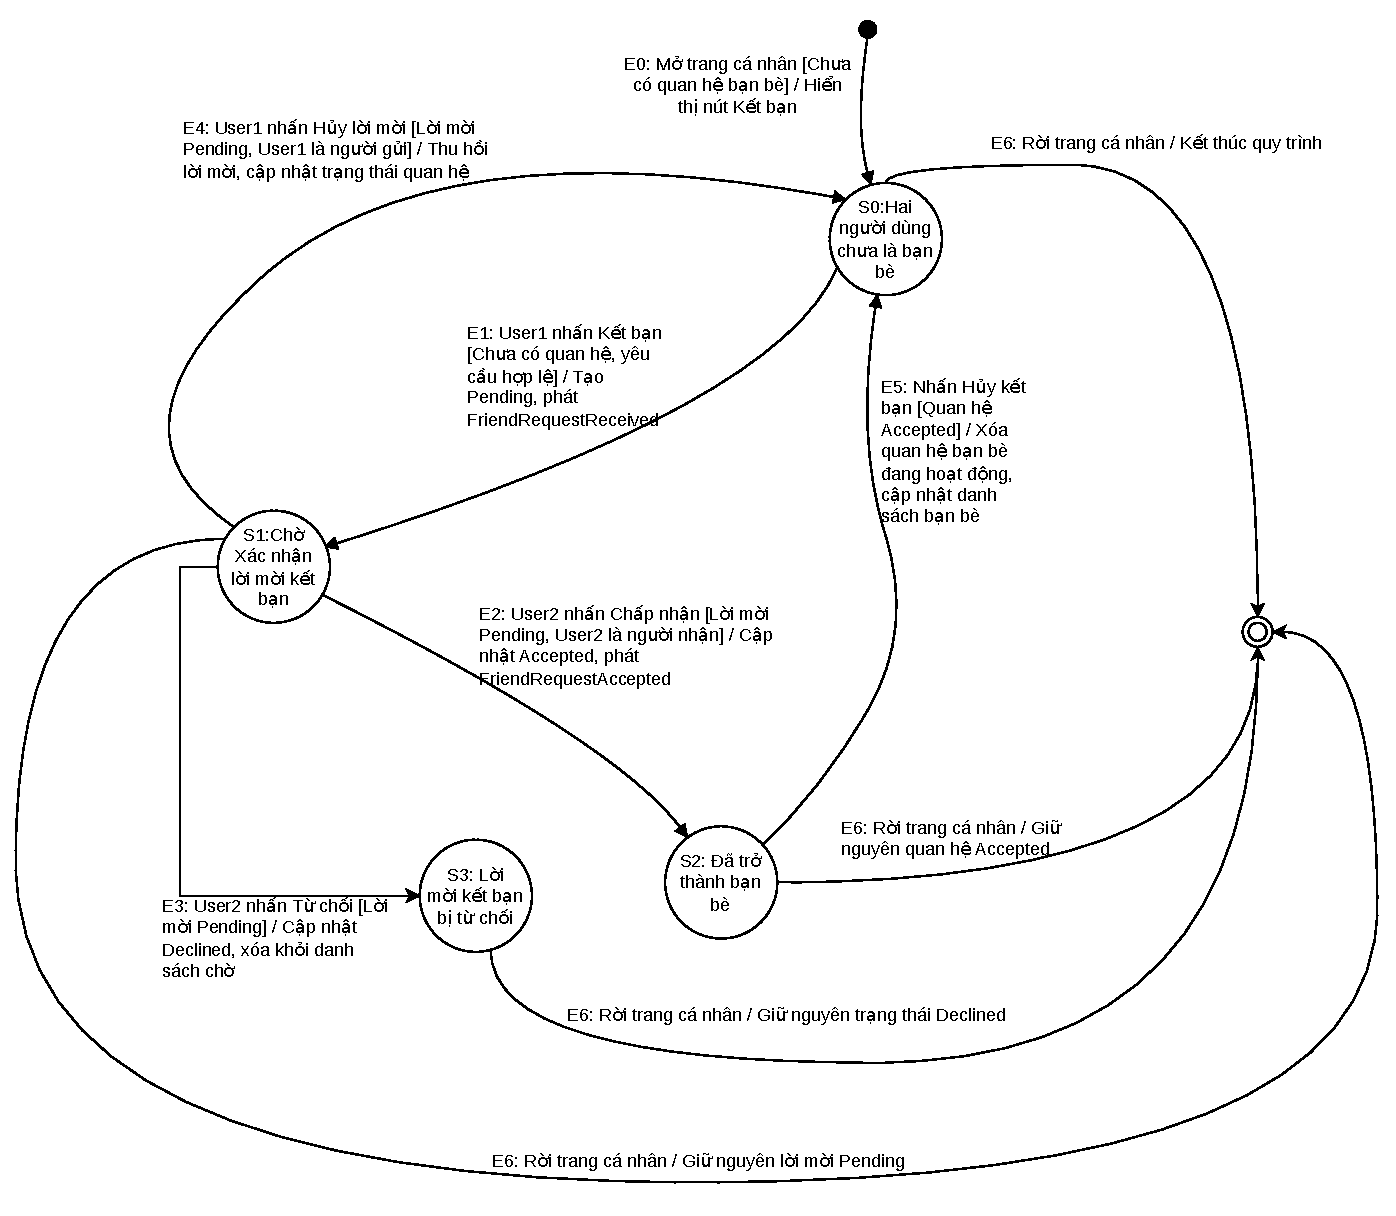
\includegraphics[width=0.92\textwidth,height=0.80\textheight,keepaspectratio]{FriendRequest.pdf}
\caption{Sơ đồ chuyển đổi trạng thái chức năng Kết bạn \& Mạng lưới kết nối (B7)}
\end{figure}

\noindent\textbf{e. Mô tả chi tiết các trạng thái}
\begin{itemize}[leftmargin=1.2cm, noitemsep]
    \item[\textbf{--}] \textbf{Chưa có quan hệ bạn bè (S0):}
    \begin{itemize}[leftmargin=0.8cm, label=--, noitemsep]
        \item \textit{Sự kiện dẫn đến:}
        \begin{itemize}[leftmargin=0.6cm, label=$\ast$, noitemsep]
            \item User1 truy cập trang cá nhân của User2 khi hai tài khoản chưa có quan hệ bạn bè.
            \item Người gửi thu hồi thành công lời mời đang chờ xử lý (\texttt{S1}).
            \item Một trong hai người thực hiện hủy kết bạn thành công (\texttt{S2}).
        \end{itemize}
        \item \textit{Hành động kèm theo:}
        \begin{itemize}[leftmargin=0.6cm, label=$\ast$, noitemsep]
            \item Hệ thống hiển thị trạng thái quan hệ chưa kết bạn.
            \item Hiển thị nút Kết bạn đối với người dùng khác.
            \item Không tồn tại quan hệ \texttt{Accepted} hoặc lời mời \texttt{Pending} giữa hai tài khoản.
            \item Cho phép gửi lời mời kết bạn hợp lệ.
        \end{itemize}
    \end{itemize}

    \item[\textbf{--}] \textbf{Chờ xác nhận lời mời kết bạn (S1):}
    \begin{itemize}[leftmargin=0.8cm, label=--, noitemsep]
        \item \textit{Sự kiện dẫn đến:}
        \begin{itemize}[leftmargin=0.6cm, label=$\ast$, noitemsep]
            \item User1 gửi lời mời kết bạn hợp lệ đến User2.
            \item Hệ thống tạo yêu cầu kết bạn ở trạng thái \texttt{Pending}.
        \end{itemize}
        \item \textit{Hành động kèm theo:}
        \begin{itemize}[leftmargin=0.6cm, label=$\ast$, noitemsep]
            \item Hệ thống lưu thông tin người gửi, người nhận và trạng thái \texttt{Pending}.
            \item Phát sự kiện \texttt{FriendRequestReceived}.
            \item User1 nhìn thấy trạng thái Đã gửi lời mời.
            \item User2 nhìn thấy lời mời với các thao tác Chấp nhận và Từ chối.
            \item Không cho phép tạo lời mời trùng lặp.
            \item Chờ người nhận chấp nhận hoặc từ chối, hoặc người gửi thu hồi lời mời theo yêu cầu hệ thống.
        \end{itemize}
    \end{itemize}

    \item[\textbf{--}] \textbf{Đã trở thành bạn bè (S2):}
    \begin{itemize}[leftmargin=0.8cm, label=--, noitemsep]
        \item \textit{Sự kiện dẫn đến:}
        \begin{itemize}[leftmargin=0.6cm, label=$\ast$, noitemsep]
            \item User2 nhấn Chấp nhận với lời mời hợp lệ ở trạng thái \texttt{Pending}.
            \item Hệ thống xử lý chấp nhận thành công.
        \end{itemize}
        \item \textit{Hành động kèm theo:}
        \begin{itemize}[leftmargin=0.6cm, label=$\ast$, noitemsep]
            \item Cập nhật trạng thái quan hệ thành \texttt{Accepted}.
            \item Thêm hai tài khoản vào danh sách bạn bè tương ứng.
            \item Phát sự kiện \texttt{FriendRequestAccepted}.
            \item Cập nhật trạng thái quan hệ trên giao diện.
            \item Cho phép thực hiện chức năng Hủy kết bạn.
            \item Không cho phép gửi lời mời mới khi quan hệ \texttt{Accepted} vẫn còn hiệu lực.
        \end{itemize}
    \end{itemize}

    \item[\textbf{--}] \textbf{Lời mời kết bạn bị từ chối (S3):}
    \begin{itemize}[leftmargin=0.8cm, label=--, noitemsep]
        \item \textit{Sự kiện dẫn đến:}
        \begin{itemize}[leftmargin=0.6cm, label=$\ast$, noitemsep]
            \item Người nhận nhấn Từ chối/Xóa đối với lời mời đang ở trạng thái \texttt{Pending}.
            \item Hệ thống xử lý từ chối thành công.
        \end{itemize}
        \item \textit{Hành động kèm theo:}
        \begin{itemize}[leftmargin=0.6cm, label=$\ast$, noitemsep]
            \item Cập nhật trạng thái lời mời thành \texttt{Declined} hoặc xóa bản ghi, tùy cách triển khai.
            \item Xóa lời mời khỏi danh sách chờ xử lý.
            \item Không tạo quan hệ bạn bè giữa hai tài khoản.
            \item Không thêm hai tài khoản vào danh sách bạn bè.
            \item Hiển thị trạng thái quan hệ phù hợp sau khi lời mời bị từ chối.
            \item Cho phép kết thúc quy trình hoặc quay lại trang cá nhân.
        \end{itemize}
    \end{itemize}
\end{itemize}

\noindent\textbf{f. Bảng kiểm thử chuyển đổi trạng thái \& Bảng Test Cases chi tiết}
\begin{table}[H]
\centering
\small
\begin{tabularx}{\textwidth}{|L{2.2cm}|X|X|X|X|X|}
\hline
\rowcolor[RGB]{179, 205, 255}
\textbf{Thành phần} & \textbf{TC1} & \textbf{TC2} & \textbf{TC3} & \textbf{TC4} & \textbf{TC5} \tabularnewline
\hline
\textbf{Start state} & S0 & S1 & S1 & S1 & S2 \\ \hline
\textbf{Input} & E1 & E2 & E3 & E4 & E5 \\ \hline
\textbf{Output} & Tạo lời mời \texttt{Pending}, phát \texttt{FriendRequest\allowbreak Received} & Cập nhật \texttt{Accepted}, phát \texttt{FriendRequest\allowbreak Accepted}, cập nhật DS bạn bè & Xử lý từ chối, không tạo quan hệ bạn bè & Hủy lời mời \texttt{Pending}, cập nhật trạng thái & Gỡ quan hệ \texttt{Accepted}, cập nhật DS bạn bè \\ \hline
\textbf{Finish state} & \textbf{S1} & \textbf{S2} & \textbf{S3} & \textbf{S0} & \textbf{S0} \\ \hline
\end{tabularx}
\caption{Bảng kiểm thử chuyển đổi trạng thái chức năng Kết bạn (B7)}
\end{table}

\noindent\textbf{Bảng Test Cases chi tiết chức năng B7 (Kết bạn \& Mạng lưới kết nối -- State Transition):}
\begingroup
\scriptsize
\setlength{\tabcolsep}{3pt}
\begin{longtable}{|C{0.8cm}|C{0.75cm}|C{0.95cm}|L{2.0cm}|L{3.0cm}|L{2.25cm}|L{2.6cm}|L{2.5cm}|C{0.85cm}|}
\hline
\rowcolor[RGB]{179, 205, 255}
\textbf{TC\#} & \textbf{BR\#} & \textbf{TR\#} & \textbf{TestCase} & \textbf{TestSteps} & \textbf{Test Data} & \textbf{Expected} & \textbf{Result} & \textbf{P/F} \tabularnewline
\hline
\endfirsthead
\hline
\rowcolor[RGB]{179, 205, 255}
\textbf{TC\#} & \textbf{BR\#} & \textbf{TR\#} & \textbf{TestCase} & \textbf{TestSteps} & \textbf{Test Data} & \textbf{Expected} & \textbf{Result} & \textbf{P/F} \tabularnewline
\hline
\endhead
\hline
\endfoot
\hline
\caption{Bảng Test Cases chức năng B7 -- Kết bạn \& Mạng lưới kết nối (State Transition)}
\endlastfoot
\textbf{120} & B7 & T99 & Gửi lời mời kết bạn và nhận thông báo qua SignalR (TC1) & 1. Mở 2 trình duyệt User1, User2\newline 2. User1 bấm ``Thêm bạn bè'' với User2 & Người gửi: User1\newline Người nhận: User2 & Lưu trạng thái chờ duyệt; User2 lập tức nhận thông báo realtime. & Lưu chờ duyệt và đẩy thông báo tức thì. & \textcolor{blue}{\textbf{Pass}} \\ \hline
\textbf{121} & B7 & T100 & Người nhận chấp nhận lời mời kết bạn (TC2) & 1. User2 mở danh sách lời mời\newline 2. Nhấp ``Xác nhận'' lời mời của User1 & Người gửi: User1\newline Người nhận: User2 & Lời mời biến mất khỏi DS chờ, cả hai xuất hiện trong DS bạn bè. & Cả hai trở thành bạn bè chính thức. & \textcolor{blue}{\textbf{Pass}} \\ \hline
\textbf{122} & B7 & T101 & Người nhận từ chối lời mời kết bạn (TC3) & 1. User2 mở tab ``Lời mời đã nhận''\newline 2. Nhấp ``Xóa'' (Từ chối) lời mời của User1 & Người gửi: User1\newline Người nhận: User2 & Lời mời bị xóa khỏi DS chờ, hai tài khoản không thành bạn bè. & Xóa khỏi DS chờ, không thành bạn bè. & \textcolor{blue}{\textbf{Pass}} \\ \hline
\textbf{123} & B7 & T102 & Người gửi thu hồi (hủy) lời mời kết bạn đã gửi (TC4) & 1. User1 vào lại trang User2 hoặc tab ``Lời mời đã gửi''\newline 2. Nhấp nút ``Hủy lời mời'' & Người gửi: User1\newline Người nhận: User2 & Nút chuyển về ``Thêm bạn bè'', xóa lời mời khỏi DS chờ của User2. & Không tồn tại nút ``Hủy lời mời'' trên UI (Defect \#9). & \textcolor{red}{\textbf{Fail}} \\ \hline
\textbf{124} & B7 & T103 & Thực hiện hủy kết bạn (Unfriend) (TC5) & 1. User1 vào trang User2 (đang là bạn bè)\newline 2. Nhấp icon hủy kết bạn và xác nhận & User1 -- User2 (Accepted) & Quan hệ chuyển về ``Thêm bạn bè'', xóa khỏi DS bạn bè cả hai phía. & Hủy kết bạn và cập nhật DS cả hai phía. & \textcolor{blue}{\textbf{Pass}} \\ \hline
\end{longtable}
\endgroup

\subsubsection{Chức năng B13 -- Báo cáo vi phạm \& Kháng cáo bài viết}

\noindent\textbf{a. Mô tả nghiệp vụ \& Yêu cầu kỹ thuật (TRD)}
\begin{itemize}[leftmargin=1.2cm, noitemsep]
    \item[\textbf{--}] \textbf{Mã BRD:} B13
    \item[\textbf{--}] \textbf{Tên chức năng:} Báo cáo vi phạm \& Kháng cáo bài viết (Content Moderation \& Appeals) -- Quy trình kiểm duyệt nội dung cộng đồng và xử lý khiếu nại giữa Người dùng (User) và Quản trị viên (Admin).
    \item[\textbf{--}] \textbf{Tóm tắt Requirement từ tài liệu hệ thống:}
    \begin{itemize}[leftmargin=0.8cm, label=$\ast$, noitemsep]
        \item Người dùng đăng nhập có quyền gửi báo cáo bài viết vi phạm tiêu chuẩn cộng đồng với các lý do cụ thể (Spam, Harassment, Inappropriate, Violence, Copyright, Other) kèm mô tả chi tiết (tối đa 500 ký tự).
        \item Người dùng không được phép tự báo cáo bài viết của chính mình; chặn gửi báo cáo trùng lặp cho cùng một bài viết đang chờ xử lý.
        \item Báo cáo mới tạo được gán trạng thái Đang chờ xử lý (\texttt{Pending}) và xuất hiện ngay trong danh sách kiểm duyệt của Admin.
        \item Admin xem danh sách toàn bộ báo cáo (\texttt{/admin/reports}) với bộ lọc trạng thái: Đang chờ, Đã gỡ bài, Đã bác bỏ, Đang kháng cáo.
        \item Admin thực hiện hành động ``Gỡ bỏ bài viết'' (Resolve): Bài viết bị ẩn khỏi Bảng tin (\texttt{IsDeleted = true}) và gửi thông báo kiểm duyệt tới tác giả.
        \item Admin thực hiện hành động ``Bác bỏ báo cáo'' (Dismiss): Bài viết được giữ nguyên trên Bảng tin, trạng thái báo cáo chuyển thành Đã bác bỏ.
        \item Tác giả có bài viết bị gỡ nhận thông báo kèm nút ``Kháng cáo''; gửi kháng cáo bắt buộc nhập lý do từ 10 đến 1.000 ký tự (chuyển sang trạng thái \texttt{Appealing}). Tác giả chỉ được kháng cáo 1 lần.
        \item Admin thẩm định kháng cáo: có quyền ``Chấp thuận kháng cáo'' (khôi phục bài viết \texttt{IsDeleted = false}) hoặc ``Từ chối kháng cáo'' (giữ nguyên quyết định gỡ bài).
    \end{itemize}
\end{itemize}

\begin{table}[H]
\centering
\small
\begin{tabularx}{\textwidth}{|C{1.5cm}|X|}
\hline
\rowcolor[RGB]{179, 205, 255}
\textbf{T\#} & \textbf{Mô tả} \tabularnewline
\hline
\textbf{T147} & Báo cáo bài viết bắt buộc chọn lý do vi phạm chuẩn; chi tiết báo cáo bắt buộc từ 10 đến 500 ký tự. \\ \hline
\textbf{T148} & Mỗi người chỉ được báo cáo một bài viết tối đa một lần; chặn gửi báo cáo trùng lặp. \\ \hline
\textbf{T149} & Báo cáo mới tạo được gán trạng thái \texttt{Pending} và xuất hiện ngay trong danh sách kiểm duyệt của Admin. \\ \hline
\textbf{T150} & Quản trị viên có trang riêng xem danh sách bài viết bị báo cáo có hỗ trợ lọc theo trạng thái: \texttt{Pending}, \texttt{Resolved}, \texttt{Dismissed}, \texttt{Appealing}. \\ \hline
\textbf{T151} & Giao diện kiểm duyệt Admin hiển thị đầy đủ: nội dung văn bản, hình ảnh đính kèm, tác giả, người báo cáo, thời gian và lý do. \\ \hline
\textbf{T152} & Admin gỡ bài vi phạm: cập nhật \texttt{IsDeleted = true}, ẩn khỏi Bảng tin, gửi thông báo kiểm duyệt tới tác giả. \\ \hline
\textbf{T153} & Admin bác bỏ báo cáo: giữ nguyên bài viết công khai, chuyển trạng thái báo cáo thành \texttt{Dismissed}. \\ \hline
\textbf{T154} & Tác giả bài viết khi bị gỡ bài do vi phạm sẽ nhìn thấy thông báo lý do gỡ bài và nút chức năng ``Kháng cáo''. \\ \hline
\textbf{T155} & Người dùng gửi đơn Kháng cáo phải nhập lý do từ 10 đến 1.000 ký tự; trạng thái của báo cáo được cập nhật thành \texttt{Appealing}. \\ \hline
\textbf{T156} & Báo cáo đang ở trạng thái Kháng cáo hiển thị nổi bật trong giao diện Admin kèm huy hiệu và trọn vẹn văn bản giải trình. \\ \hline
\textbf{T157} & Admin chấp thuận kháng cáo: tự động khôi phục bài viết về trạng thái công khai (\texttt{IsDeleted = false}), thông báo chúc mừng tới tác giả. \\ \hline
\textbf{T158} & Admin từ chối kháng cáo: giữ nguyên trạng thái gỡ bỏ bài viết, cập nhật Kháng cáo bị từ chối; tác giả chỉ được gửi kháng cáo 1 lần duy nhất. \\ \hline
\end{tabularx}
\caption{Bảng TRD liên quan chức năng Báo cáo vi phạm \& Kháng cáo (\texttt{T147--T158})}
\end{table}

\noindent\textbf{b. Định nghĩa các trạng thái (\texttt{S0--S6})}

\begin{table}[H]
\centering
\small
\begin{tabularx}{\textwidth}{|C{2.4cm}|L{4.8cm}|X|}
\hline
\rowcolor[RGB]{179, 205, 255}
\textbf{Mã trạng thái} & \textbf{Tên trạng thái} & \textbf{Mô tả} \tabularnewline
\hline
\textbf{S0} & Bài viết công khai bình thường & Bài viết hiển thị công khai trên Bảng tin, chưa có báo cáo vi phạm nào đang chờ xử lý. \\ \hline
\textbf{S1} & Đang chờ xử lý báo cáo (\texttt{Pending}) & Người dùng đã gửi báo cáo vi phạm hợp lệ; bài viết xuất hiện trong danh sách duyệt của Admin. \\ \hline
\textbf{S2} & Báo cáo bị bác bỏ (\texttt{Dismissed}) & Admin thẩm định thấy bài viết không vi phạm; báo cáo đóng lại, bài viết giữ nguyên công khai. \\ \hline
\textbf{S3} & Bài viết bị gỡ bỏ vi phạm (\texttt{Resolved}) & Admin xác nhận vi phạm và gỡ bài (\texttt{IsDeleted = true}); gửi thông báo kèm nút Kháng cáo cho tác giả. \\ \hline
\textbf{S4} & Đang kháng cáo (\texttt{Appealing}) & Tác giả đã gửi giải trình kháng cáo hợp lệ (10--1.000 ký tự); báo cáo hiển thị nổi bật chờ Admin thẩm định lại. \\ \hline
\textbf{S5} & Kháng cáo được chấp thuận (\texttt{Appeal Accepted}) & Admin đồng ý kháng cáo; bài viết được khôi phục công khai trên Bảng tin (\texttt{IsDeleted = false}). \\ \hline
\textbf{S6} & Kháng cáo bị từ chối (\texttt{Appeal Rejected}) & Admin bác bỏ kháng cáo; bài viết bị gỡ vĩnh viễn; khóa quyền kháng cáo tiếp theo của tác giả. \\ \hline
\end{tabularx}
\caption{Bảng định nghĩa 7 trạng thái của chức năng Báo cáo vi phạm \& Kháng cáo (B13)}
\end{table}

\noindent\textbf{c. Liệt kê các luồng nghiệp vụ}
\begin{itemize}[leftmargin=1.2cm, noitemsep]
    \item[\textbf{--}] \textbf{Luồng 1 -- Gửi báo cáo vi phạm bài viết thành công} (\textit{Sequence of States:} $\text{Start} \rightarrow \text{S0} \rightarrow \text{S1}$):
    \begin{enumerate}[leftmargin=0.7cm, noitemsep]
        \item User1 lướt Bảng tin thấy bài viết ID \#10 của User2 có nội dung vi phạm.
        \item User1 nhấp menu ba chấm của bài viết, chọn ``Báo cáo bài viết''.
        \item User1 chọn lý do ``Nội dung quấy rối'' và nhập mô tả chi tiết hợp lệ 50 ký tự.
        \item User1 nhấn nút ``Gửi báo cáo'' (\texttt{E1}).
        \item Hệ thống kiểm tra hợp lệ, ghi nhận báo cáo vào CSDL ở trạng thái \texttt{Pending} (\texttt{S1}).
        \item Báo cáo lập tức hiển thị trong danh sách kiểm duyệt của Quản trị viên.
    \end{enumerate}

    \item[\textbf{--}] \textbf{Luồng 2 -- Admin bác bỏ báo cáo vi phạm không chính xác} (\textit{Sequence of States:} $\text{Start} \rightarrow \text{S1} \rightarrow \text{S2} \rightarrow \text{End}$):
    \begin{enumerate}[leftmargin=0.7cm, noitemsep]
        \item Quản trị viên đăng nhập vào \texttt{/admin/reports} và xem xét báo cáo của bài viết ID \#18 (\texttt{S1}).
        \item Quản trị viên xem chi tiết và nhận định bài viết hoàn toàn hợp lệ, không vi phạm tiêu chuẩn cộng đồng.
        \item Quản trị viên nhấn nút ``Bác bỏ báo cáo'' (màu xám) và xác nhận (\texttt{E3}).
        \item Hệ thống cập nhật trạng thái báo cáo thành \texttt{Dismissed} (\texttt{S2}).
        \item Bài viết ID \#18 vẫn tiếp tục hiển thị bình thường trên Bảng tin.
    \end{enumerate}

    \item[\textbf{--}] \textbf{Luồng 3 -- Admin duyệt báo cáo và gỡ bỏ bài viết vi phạm} (\textit{Sequence of States:} $\text{Start} \rightarrow \text{S1} \rightarrow \text{S3}$):
    \begin{enumerate}[leftmargin=0.7cm, noitemsep]
        \item Quản trị viên xem báo cáo bài viết ID \#15 đang ở trạng thái \texttt{Pending} (\texttt{S1}).
        \item Quản trị viên kiểm tra nội dung và xác định bài viết vi phạm nghiêm trọng.
        \item Quản trị viên nhấn nút ``Gỡ bỏ bài viết'' (màu đỏ) và bấm ``Duyệt báo cáo'' (\texttt{E4}).
        \item Hệ thống cập nhật bài viết thành \texttt{IsDeleted = true}, trạng thái báo cáo chuyển thành \texttt{Resolved} (\texttt{S3}).
        \item Bài viết lập tức biến mất khỏi Bảng tin của mọi người dùng.
        \item Hệ thống tự động gửi thông báo kiểm duyệt kèm nút ``Kháng cáo'' màu xanh tới tác giả bài viết.
    \end{enumerate}

    \item[\textbf{--}] \textbf{Luồng 4 -- Tác giả gửi yêu cầu kháng cáo thành công} (\textit{Sequence of States:} $\text{Start} \rightarrow \text{S3} \rightarrow \text{S4}$):
    \begin{enumerate}[leftmargin=0.7cm, noitemsep]
        \item Tác giả bài viết ID \#15 mở thông báo kiểm duyệt và nhấp vào nút ``Kháng cáo''.
        \item Biểu mẫu kháng cáo hiển thị. Tác giả nhập văn bản giải trình hợp lệ 68 ký tự.
        \item Tác giả bấm ``Gửi kháng cáo'' (\texttt{E5}).
        \item Hệ thống xác thực độ dài hợp lệ (10--1.000 ký tự) và tác giả chưa từng gửi kháng cáo trước đó.
        \item Hệ thống cập nhật trạng thái báo cáo thành \texttt{Appealing} (\texttt{S4}).
        \item Báo cáo xuất hiện nổi bật với huy hiệu cảnh báo trong trang quản trị Admin.
    \end{enumerate}

    \item[\textbf{--}] \textbf{Luồng 5 -- Admin chấp thuận kháng cáo và khôi phục bài viết} (\textit{Sequence of States:} $\text{Start} \rightarrow \text{S4} \rightarrow \text{S5} \rightarrow \text{End}$):
    \begin{enumerate}[leftmargin=0.7cm, noitemsep]
        \item Quản trị viên lọc danh sách báo cáo theo trạng thái ``Đang kháng cáo'' (\texttt{S4}).
        \item Quản trị viên mở xem chi tiết bài viết ID \#15 và đọc toàn văn bản giải trình của tác giả.
        \item Quản trị viên nhận thấy lý do giải trình chính đáng và nhấn ``Chấp thuận kháng cáo'' (nút màu xanh lá) (\texttt{E6}).
        \item Hệ thống khôi phục trạng thái bài viết (\texttt{IsDeleted = false}), cập nhật báo cáo thành Kháng cáo thành công (\texttt{S5}).
        \item Bài viết tự động xuất hiện trở lại trên Bảng tin công khai.
        \item Hệ thống gửi thông báo chúc mừng tới tác giả bài viết.
    \end{enumerate}

    \item[\textbf{--}] \textbf{Luồng 6 -- Admin từ chối kháng cáo của người dùng} (\textit{Sequence of States:} $\text{Start} \rightarrow \text{S4} \rightarrow \text{S6} \rightarrow \text{End}$):
    \begin{enumerate}[leftmargin=0.7cm, noitemsep]
        \item Quản trị viên xem xét một báo cáo đang kháng cáo nhưng giải trình không thỏa đáng (\texttt{S4}).
        \item Quản trị viên nhấp vào nút ``Từ chối kháng cáo'' (màu đỏ), nhập lý do từ chối và bấm xác nhận (\texttt{E7}).
        \item Hệ thống giữ nguyên trạng thái gỡ bỏ bài viết (\texttt{IsDeleted = true}), chuyển báo cáo thành Kháng cáo bị từ chối (\texttt{S6}).
        \item Hệ thống gửi thông báo giải thích quyết định cuối cùng tới tác giả; khóa tính năng kháng cáo lần hai đối với bài viết này.
    \end{enumerate}

    \item[\textbf{--}] \textbf{Luồng 7 -- Chặn gửi báo cáo trùng lặp} (\textit{Sequence of States:} $\text{Start} \rightarrow \text{S1} \rightarrow \text{S1}$ (duy trì \texttt{S1})):
    \begin{enumerate}[leftmargin=0.7cm, noitemsep]
        \item User1 vừa gửi báo cáo bài viết ID \#10 thành công (báo cáo đang ở \texttt{S1} -- \texttt{Pending}).
        \item User1 lại nhấp menu ba chấm của chính bài viết ID \#10 và chọn ``Báo cáo bài viết'', bấm Gửi lần nữa (\texttt{E2}).
        \item Hệ thống kiểm tra thấy đã tồn tại báo cáo đang chờ xử lý từ User1 cho bài viết này.
        \item Hệ thống chặn gửi và cảnh báo: ``Bạn đã gửi báo cáo cho bài viết này rồi, vui lòng chờ Quản trị viên xử lý''.
    \end{enumerate}
\end{itemize}

\noindent\textbf{d. Sơ đồ chuyển đổi trạng thái}
\begin{figure}[H]
\centering
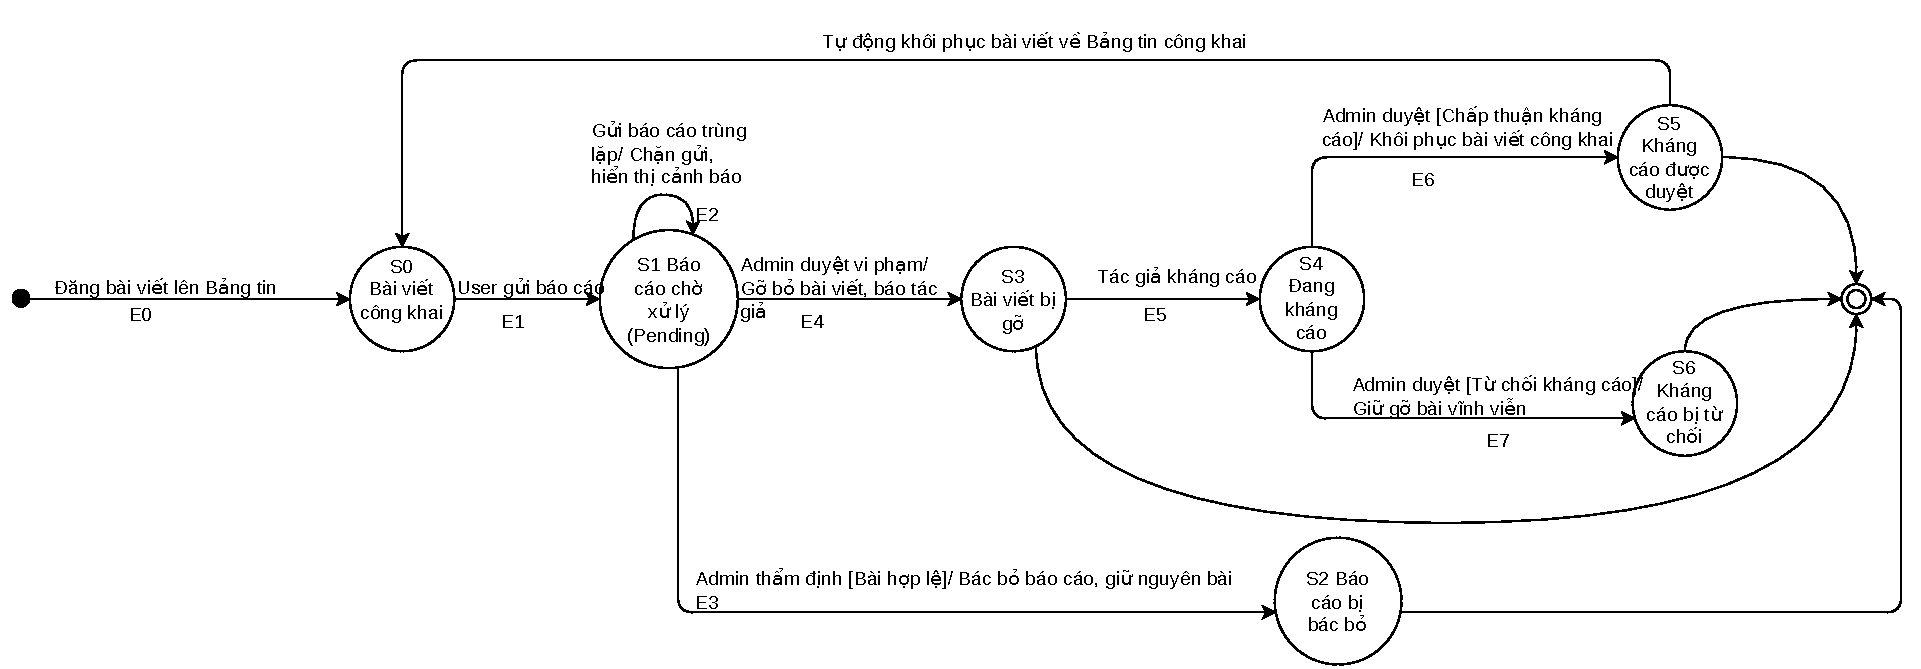
\includegraphics[width=1.07\textwidth,height=0.80\textheight,keepaspectratio]{Report.pdf}
\caption{Sơ đồ chuyển đổi trạng thái chức năng Báo cáo vi phạm \& Kháng cáo (B13)}
\end{figure}

\noindent\textbf{e. Mô tả chi tiết các trạng thái}
\begin{itemize}[leftmargin=1.2cm, noitemsep]
    \item[\textbf{--}] \textbf{Bài viết công khai bình thường (S0):}
    \begin{itemize}[leftmargin=0.8cm, label=--, noitemsep]
        \item \textit{Sự kiện dẫn đến:}
        \begin{itemize}[leftmargin=0.6cm, label=$\ast$, noitemsep]
            \item Bài viết được người dùng đăng tải công khai thành công trên Bảng tin (\texttt{E0}).
        \end{itemize}
        \item \textit{Hành động kèm theo:}
        \begin{itemize}[leftmargin=0.6cm, label=$\ast$, noitemsep]
            \item Bài viết hiển thị bình thường cho mọi người dùng.
            \item Menu 3 chấm hiển thị tùy chọn ``Báo cáo bài viết'' cho người xem (không hiển thị cho chính tác giả).
        \end{itemize}
    \end{itemize}

    \item[\textbf{--}] \textbf{Đang chờ xử lý báo cáo -- Pending (S1):}
    \begin{itemize}[leftmargin=0.8cm, label=--, noitemsep]
        \item \textit{Sự kiện dẫn đến:}
        \begin{itemize}[leftmargin=0.6cm, label=$\ast$, noitemsep]
            \item Người dùng gửi báo cáo vi phạm hợp lệ với lý do bắt buộc và mô tả chi tiết (\texttt{E1}).
        \end{itemize}
        \item \textit{Hành động kèm theo:}
        \begin{itemize}[leftmargin=0.6cm, label=$\ast$, noitemsep]
            \item Lưu bản ghi báo cáo vào CSDL với trạng thái \texttt{Pending}.
            \item Xuất hiện trong danh sách kiểm duyệt của Quản trị viên với huy hiệu màu cam.
            \item Chặn người dùng đó tiếp tục gửi báo cáo trùng lặp cho bài viết này (\texttt{E2}).
        \end{itemize}
    \end{itemize}

    \item[\textbf{--}] \textbf{Báo cáo bị bác bỏ -- Dismissed (S2):}
    \begin{itemize}[leftmargin=0.8cm, label=--, noitemsep]
        \item \textit{Sự kiện dẫn đến:}
        \begin{itemize}[leftmargin=0.6cm, label=$\ast$, noitemsep]
            \item Quản trị viên nhấn nút ``Bác bỏ báo cáo'' trong giao diện kiểm duyệt (\texttt{E3}).
        \end{itemize}
        \item \textit{Hành động kèm theo:}
        \begin{itemize}[leftmargin=0.6cm, label=$\ast$, noitemsep]
            \item Cập nhật trạng thái báo cáo thành \texttt{Dismissed}.
            \item Giữ nguyên bài viết công khai trên Bảng tin, không ảnh hưởng đến tài khoản tác giả.
        \end{itemize}
    \end{itemize}

    \item[\textbf{--}] \textbf{Bài viết bị gỡ bỏ vi phạm -- Resolved (S3):}
    \begin{itemize}[leftmargin=0.8cm, label=--, noitemsep]
        \item \textit{Sự kiện dẫn đến:}
        \begin{itemize}[leftmargin=0.6cm, label=$\ast$, noitemsep]
            \item Quản trị viên nhấn nút ``Gỡ bỏ bài viết'' sau khi xác nhận vi phạm (\texttt{E4}).
        \end{itemize}
        \item \textit{Hành động kèm theo:}
        \begin{itemize}[leftmargin=0.6cm, label=$\ast$, noitemsep]
            \item Cập nhật trạng thái bài viết thành \texttt{IsDeleted = true}.
            \item Bài viết lập tức biến mất khỏi Bảng tin, trang cá nhân và nhóm.
            \item Gửi thông báo kiểm duyệt đến tác giả kèm nút ``Kháng cáo'' màu xanh.
        \end{itemize}
    \end{itemize}

    \item[\textbf{--}] \textbf{Đang kháng cáo -- Appealing (S4):}
    \begin{itemize}[leftmargin=0.8cm, label=--, noitemsep]
        \item \textit{Sự kiện dẫn đến:}
        \begin{itemize}[leftmargin=0.6cm, label=$\ast$, noitemsep]
            \item Tác giả bài viết gửi đơn khiếu nại với lý do giải trình hợp lệ từ 10--1.000 ký tự (\texttt{E5}).
        \end{itemize}
        \item \textit{Hành động kèm theo:}
        \begin{itemize}[leftmargin=0.6cm, label=$\ast$, noitemsep]
            \item Cập nhật trạng thái báo cáo thành \texttt{Appealing}.
            \item Hiển thị nổi bật báo cáo trong danh sách Admin với huy hiệu màu vàng/cam ``Đang kháng cáo''.
            \item Hiển thị toàn văn nội dung giải trình cùng các nút ``Chấp thuận kháng cáo'' và ``Từ chối kháng cáo''.
        \end{itemize}
    \end{itemize}

    \item[\textbf{--}] \textbf{Kháng cáo được chấp thuận -- Appeal Accepted (S5):}
    \begin{itemize}[leftmargin=0.8cm, label=--, noitemsep]
        \item \textit{Sự kiện dẫn đến:}
        \begin{itemize}[leftmargin=0.6cm, label=$\ast$, noitemsep]
            \item Quản trị viên nhấn nút ``Chấp thuận kháng cáo'' (\texttt{E6}).
        \end{itemize}
        \item \textit{Hành động kèm theo:}
        \begin{itemize}[leftmargin=0.6cm, label=$\ast$, noitemsep]
            \item Tự động khôi phục bài viết về trạng thái công khai (\texttt{IsDeleted = false}).
            \item Bài viết xuất hiện trở lại trên Bảng tin; gửi thông báo chúc mừng tới tác giả.
        \end{itemize}
    \end{itemize}

    \item[\textbf{--}] \textbf{Kháng cáo bị từ chối -- Appeal Rejected (S6):}
    \begin{itemize}[leftmargin=0.8cm, label=--, noitemsep]
        \item \textit{Sự kiện dẫn đến:}
        \begin{itemize}[leftmargin=0.6cm, label=$\ast$, noitemsep]
            \item Quản trị viên nhấn nút ``Từ chối kháng cáo'' (\texttt{E7}).
        \end{itemize}
        \item \textit{Hành động kèm theo:}
        \begin{itemize}[leftmargin=0.6cm, label=$\ast$, noitemsep]
            \item Giữ nguyên trạng thái gỡ bỏ bài viết vĩnh viễn; khóa quyền khiếu nại tiếp theo của tác giả.
            \item Gửi thông báo giải thích quyết định cuối cùng tới tác giả.
        \end{itemize}
    \end{itemize}
\end{itemize}

\noindent\textbf{f. Bảng kiểm thử chuyển đổi trạng thái \& Bảng Test Cases chi tiết}
\begin{table}[H]
\centering
\small
\begin{tabularx}{\textwidth}{|L{1.9cm}|X|X|X|X|X|X|X|}
\hline
\rowcolor[RGB]{179, 205, 255}
\textbf{Thành phần} & \textbf{TC1} & \textbf{TC2} & \textbf{TC3} & \textbf{TC4} & \textbf{TC5} & \textbf{TC6} & \textbf{TC7} \tabularnewline
\hline
\textbf{Start state} & S0 & S1 & S1 & S1 & S3 & S4 & S4 \\ \hline
\textbf{Input} & E1 & E2 & E3 & E4 & E5 & E6 & E7 \\ \hline
\textbf{Output} & Tạo báo cáo \texttt{Pending}, gửi Admin & Chặn gửi báo cáo trùng & Bác bỏ, giữ nguyên bài & \texttt{IsDeleted\allowbreak =true}, ẩn bài, báo tác giả & Chuyển \texttt{Appealing}, hiện badge Admin & \texttt{IsDeleted\allowbreak =false}, khôi phục bài & Giữ gỡ vĩnh viễn, khóa kháng cáo \\ \hline
\textbf{Finish state} & \textbf{S1} & \textbf{S1} & \textbf{S2} & \textbf{S3} & \textbf{S4} & \textbf{S5} & \textbf{S6} \\ \hline
\end{tabularx}
\caption{Bảng kiểm thử chuyển đổi trạng thái Báo cáo \& Kháng cáo (B13)}
\end{table}


\pagebreak
\noindent\textbf{Bảng Test Cases chi tiết chức năng B13 (Báo cáo vi phạm \& Kháng cáo -- State Transition):}
\begingroup
\scriptsize
\setlength{\tabcolsep}{3pt}
\begin{longtable}{|C{0.8cm}|C{0.75cm}|C{0.95cm}|L{2.0cm}|L{3.0cm}|L{2.25cm}|L{2.6cm}|L{2.5cm}|C{0.85cm}|}
\hline
\rowcolor[RGB]{179, 205, 255}
\textbf{TC\#} & \textbf{BR\#} & \textbf{TR\#} & \textbf{TestCase} & \textbf{TestSteps} & \textbf{Test Data} & \textbf{Expected} & \textbf{Result} & \textbf{P/F} \tabularnewline
\hline
\endfirsthead
\hline
\rowcolor[RGB]{179, 205, 255}
\textbf{TC\#} & \textbf{BR\#} & \textbf{TR\#} & \textbf{TestCase} & \textbf{TestSteps} & \textbf{Test Data} & \textbf{Expected} & \textbf{Result} & \textbf{P/F} \tabularnewline
\hline
\endhead
\hline
\endfoot
\hline
\caption{Bảng Test Cases chức năng B13 -- Báo cáo vi phạm \& Kháng cáo (State Transition)}
\endlastfoot
\textbf{205} & B13 & T147 & Báo cáo bài viết vi phạm với lý do và mô tả hợp lệ (TC1) & 1. Nhấp menu 3 chấm bài viết, chọn ``Báo cáo bài viết''\newline 2. Chọn lý do, nhập mô tả $< 500$ kt, bấm Gửi & Bài ID \#10\newline Lý do: Nội dung quấy rối & Hộp thoại đóng lại, báo cáo được gửi đến Admin. & Hộp thoại đóng lại, gửi báo cáo thành công. & \textcolor{blue}{\textbf{Pass}} \\ \hline
\textbf{206} & B13 & T148 & Chặn gửi báo cáo trùng lặp cho cùng bài đang chờ duyệt (TC2) & 1. Vừa báo cáo bài ID \#10 thành công\newline 2. Tiếp tục mở menu báo cáo lại chính bài \#10 & Bài ID \#10 (đang Pending) & Cảnh báo ``Bạn đã gửi báo cáo cho bài viết này rồi...'' và chặn gửi. & Hộp thoại đóng lại, vẫn gửi trùng được đến Admin (Defect \#15). & \textcolor{red}{\textbf{Fail}} \\ \hline
\textbf{210} & B13 & T152 & Admin thực hiện gỡ bỏ bài viết vi phạm (TC4) & 1. Mở chi tiết báo cáo bài \#15\newline 2. Nhấp ``Gỡ bỏ bài viết'' và xác nhận & Báo cáo bài ID \#15 & Trạng thái chuyển thành ``Đã duyệt'' (Resolved), bài biến mất khỏi Feed. & Bài bị gỡ bỏ và ẩn khỏi Bảng tin. & \textcolor{blue}{\textbf{Pass}} \\ \hline
\textbf{211} & B13 & T153 & Admin bác bỏ báo cáo vi phạm không chính xác (TC3) & 1. Xem báo cáo bài \#18 không vi phạm\newline 2. Nhấp ``Bác bỏ báo cáo'' và xác nhận & Báo cáo bài ID \#18 & Trạng thái chuyển thành ``Đã bác bỏ'' (Dismissed), giữ nguyên bài. & Bác bỏ thành công, bài vẫn hiển thị. & \textcolor{blue}{\textbf{Pass}} \\ \hline
\textbf{213} & B13 & T155 & Gửi yêu cầu kháng cáo với độ dài lý do hợp lệ (TC5) & 1. Nhấp ``Kháng cáo'', thử nhập $< 10$ kt (báo lỗi)\newline 2. Nhập giải trình 68 kt, bấm Gửi & Lý do: 68 ký tự hợp lệ & Chặn khi $< 10$ kt; chấp nhận khi hợp lệ và chuyển sang ``Đang kháng cáo''. & Gửi kháng cáo thành công, chuyển trạng thái Appealing. & \textcolor{blue}{\textbf{Pass}} \\ \hline
\textbf{215} & B13 & T157 & Admin chấp thuận kháng cáo và khôi phục bài viết (TC6) & 1. Mở kháng cáo bài \#15\newline 2. Nhấp ``Chấp thuận kháng cáo'' và xác nhận & Báo cáo bài ID \#15 & Bài \#15 tự động khôi phục công khai trên Feed, báo chúc mừng tác giả. & Bài được khôi phục công khai, gửi thông báo. & \textcolor{blue}{\textbf{Pass}} \\ \hline
\textbf{216} & B13 & T158 & Admin từ chối kháng cáo và giữ nguyên gỡ bỏ (TC7) & 1. Mở kháng cáo không hợp lệ\newline 2. Nhấp ``Từ chối kháng cáo'', nhập lý do, xác nhận & Báo cáo vi phạm thực tế & Chuyển thành ``Kháng cáo bị từ chối'', giữ gỡ bài vĩnh viễn, khóa kháng cáo lại. & Từ chối kháng cáo, giữ gỡ bỏ bài viết. & \textcolor{blue}{\textbf{Pass}} \\ \hline
\end{longtable}
\endgroup

% ----------------------------------------------------------
% 3.6 Cause-Effect Graph
% ----------------------------------------------------------
\subsection{Đồ thị nhân -- quả (Cause--Effect Graph)}

\subsubsection{Chức năng B1 -- Đăng nhập người dùng}

\noindent\textbf{a. Mô tả nghiệp vụ \& Yêu cầu kỹ thuật (TRD)}
\begin{itemize}[leftmargin=1.2cm, noitemsep]
    \item[\textbf{--}] \textbf{Mã BRD:} B1
    \item[\textbf{--}] \textbf{Tên chức năng:} Đăng nhập người dùng (\texttt{User Login}) -- Kiểm tra điều kiện xác thực và phân quyền cổng đăng nhập.
    \item[\textbf{--}] \textbf{Tóm tắt Requirement từ tài liệu hệ thống:}
    \begin{itemize}[leftmargin=0.8cm, label=$\bullet$, noitemsep]
        \item Tên đăng nhập và mật khẩu không được để trống.
        \item Tài khoản phải tồn tại trong hệ thống và mật khẩu phải trùng khớp.
        \item Tài khoản có vai trò Quản trị viên (\texttt{Admin}) không được phép đăng nhập qua cổng người dùng thường.
        \item Khi hợp lệ, hệ thống cho phép đăng nhập, lưu phiên 60 phút và chuyển hướng về trang chủ; khi sai thông tin, hiển thị thông báo lỗi chung để bảo mật.
    \end{itemize}
\end{itemize}

\begin{table}[H]
\centering
\small
\begin{tabularx}{\textwidth}{|C{1.8cm}|X|}
\hline
\rowcolor[RGB]{179, 205, 255}
\textbf{T\#} & \textbf{Mô tả yêu cầu} \tabularnewline
\hline
\textbf{T01--T02} & Tên đăng nhập và mật khẩu không được để trống. \\ \hline
\textbf{T03--T04} & Tài khoản phải tồn tại trong hệ thống và mật khẩu nhập vào phải trùng khớp. \\ \hline
\textbf{T05} & Tài khoản Quản trị viên (\texttt{Admin}) không được phép đăng nhập ở cổng người dùng thường. \\ \hline
\textbf{T06--T07} & Hợp lệ thì cấp phiên đăng nhập 60 phút; sai tên đăng nhập hoặc mật khẩu thì từ chối và báo lỗi chung. \\ \hline
\end{tabularx}
\caption{Bảng mã yêu cầu kỹ thuật chức năng Đăng nhập người dùng (B1)}
\end{table}

\noindent\textbf{b. Xác định Nguyên nhân (Causes) \& Kết quả (Effects)}
\begin{table}[H]
\centering
\small
\begin{minipage}[t]{0.48\textwidth}
\begin{tabularx}{\linewidth}{|C{1.3cm}|X|}
\hline
\rowcolor[RGB]{179, 205, 255}
\textbf{Mã} & \textbf{Nguyên nhân (Causes)} \tabularnewline
\hline
\textbf{C1} & Tên đăng nhập hợp lệ (không trống) \\ \hline
\textbf{C2} & Mật khẩu hợp lệ (không trống) \\ \hline
\textbf{C3} & Tài khoản tồn tại trong hệ thống \\ \hline
\textbf{C4} & Tài khoản không có vai trò \texttt{Admin} \\ \hline
\textbf{C5} & Mật khẩu trùng khớp với tài khoản \\ \hline
\end{tabularx}
\caption{Danh sách nguyên nhân (\texttt{C1}--\texttt{C5}) chức năng B1}
\end{minipage}\hfill
\begin{minipage}[t]{0.48\textwidth}
\begin{tabularx}{\linewidth}{|C{1.3cm}|X|}
\hline
\rowcolor[RGB]{179, 205, 255}
\textbf{Mã} & \textbf{Kết quả (Effects)} \tabularnewline
\hline
\textbf{E1} & Đăng nhập thành công, cấp phiên \& vào \texttt{/home} \\ \hline
\textbf{E2} & Chặn gửi, báo lỗi thiếu trường bắt buộc \\ \hline
\textbf{E3} & Từ chối, báo lỗi chung sai thông tin \\ \hline
\textbf{E4} & Chặn đăng nhập, yêu cầu dùng cổng Admin \\ \hline
\end{tabularx}
\caption{Danh sách kết quả (\texttt{E1}--\texttt{E4}) chức năng B1}
\end{minipage}
\end{table}

\begin{itemize}[leftmargin=1.2cm, noitemsep]
    \item[\textbf{--}] \textbf{Gọi:}
    \begin{itemize}[leftmargin=0.8cm, label=$\bullet$, noitemsep]
        \item $M1 = C3 \land C5$
    \end{itemize}
    \item[\textbf{--}] \textbf{Biểu thức logic dẫn xuất:}
    \begin{itemize}[leftmargin=0.8cm, label=$\bullet$, noitemsep]
        \item $E1 = C1 \land C2 \land C3 \land C4 \land C5$
        \item $E2 = \neg C1 \lor \neg C2$
        \item $E3 = C1 \land C2 \land \neg M1 = C1 \land C2 \land \neg( C3 \land C5)$
        \item $E4 = C1 \land C2 \land C3 \land \neg C4 \land C5$
    \end{itemize}
\end{itemize}

\pagebreak
\noindent\textbf{c. Đồ thị nhân -- quả (Cause--Effect Graph)}
\begin{figure}[H]
\centering
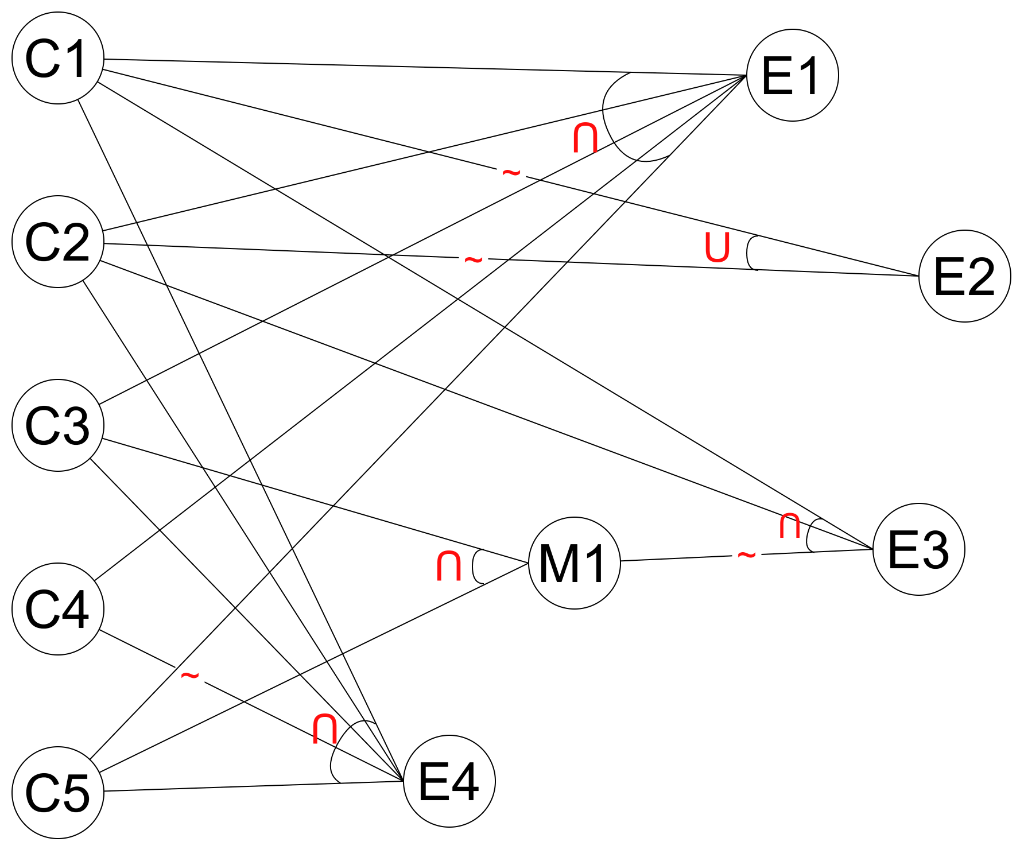
\includegraphics[width=0.82\textwidth,keepaspectratio]{CauseEffect_B1.png}
\caption{Đồ thị nhân -- quả chức năng Đăng nhập người dùng (B1)}
\end{figure}

\noindent -- Bảng quyết định dẫn xuất (\texttt{R1}--\texttt{R5}):
\begin{table}[H]
\centering
\small
\begin{tabularx}{\textwidth}{|X|C{1.1cm}|C{1.1cm}|C{1.1cm}|C{1.1cm}|C{1.1cm}|}
\hline
\rowcolor[RGB]{179, 205, 255}
\textbf{Conditions \& Actions} & \textbf{R1} & \textbf{R2} & \textbf{R3} & \textbf{R4} & \textbf{R5} \tabularnewline
\hline
\multicolumn{6}{|l|}{\cellcolor{tableheader}\textbf{Conditions}} \\ \hline
C1: Tên đăng nhập hợp lệ (không trống)? & N & Y & Y & Y & Y \\ \hline
C2: Mật khẩu hợp lệ (không trống)? & -- & Y & Y & Y & Y \\ \hline
C3: Tài khoản tồn tại trong hệ thống? & -- & N & Y & Y & Y \\ \hline
C4: Tài khoản không có vai trò \texttt{Admin}? & -- & -- & N & Y & Y \\ \hline
C5: Mật khẩu trùng khớp với tài khoản? & -- & -- & Y & N & Y \\ \hline
\multicolumn{6}{|l|}{\cellcolor{tableheader}\textbf{Actions}} \\ \hline
E1: Đăng nhập thành công, cấp phiên \& vào \texttt{/home} & & & & & \textbf{X} \\ \hline
E2: Chặn gửi, báo lỗi thiếu trường bắt buộc & \textbf{X} & & & & \\ \hline
E3: Từ chối, báo lỗi chung sai thông tin & & \textbf{X} & & \textbf{X} & \\ \hline
E4: Chặn đăng nhập, yêu cầu dùng cổng Admin & & & \textbf{X} & & \\ \hline
\rowcolor{gray!15}
\textbf{Ánh xạ Test Case} & 1 & 4 & 9 & 5 & 6 \\ \hline
\end{tabularx}
\caption{Bảng quyết định dẫn xuất (\texttt{R1}--\texttt{R5}) từ Đồ thị nhân -- quả chức năng Đăng nhập (B1)}
\end{table}

\pagebreak
\noindent\textbf{d. Bảng Test Cases chi tiết chức năng B1 (Đăng nhập người dùng):}
\begingroup
\scriptsize
\setlength{\tabcolsep}{3pt}
\renewcommand{\arraystretch}{0.88}
\begin{longtable}{|C{0.8cm}|C{0.85cm}|C{0.95cm}|L{2.0cm}|L{3.0cm}|L{2.15cm}|L{2.6cm}|L{2.5cm}|C{0.85cm}|}
\hline
\rowcolor[RGB]{179, 205, 255}
\textbf{TC\#} & \textbf{BR\#} & \textbf{TR\#} & \textbf{TestCase} & \textbf{TestSteps} & \textbf{Test Data} & \textbf{Expected} & \textbf{Result} & \textbf{P/F} \tabularnewline
\hline
\endfirsthead
\hline
\rowcolor[RGB]{179, 205, 255}
\textbf{TC\#} & \textbf{BR\#} & \textbf{TR\#} & \textbf{TestCase} & \textbf{TestSteps} & \textbf{Test Data} & \textbf{Expected} & \textbf{Result} & \textbf{P/F} \tabularnewline
\hline
\endhead
\hline
\endfoot
\hline
\caption{Bảng Test Cases chức năng B1 -- Đăng nhập người dùng (Cause--Effect Graph)}
\endlastfoot
\textbf{1} & B1 & T01 & Đăng nhập khi bỏ trống Tên đăng nhập (R1) & 1. Vào trang đăng nhập\newline 2. Để trống Tên đăng nhập, nhập MK, bấm Đăng nhập & Tên: (trống)\newline MK: User@123456 & Chặn gửi và yêu cầu nhập Tên đăng nhập. & Trình duyệt chặn gửi, báo bắt buộc nhập. & \textcolor{blue}{\textbf{Pass}} \\ \hline
\textbf{4} & B1 & T03, T07 & Đăng nhập với tài khoản không tồn tại (R2) & 1. Nhập tên không tồn tại và MK bất kỳ\newline 2. Bấm Đăng nhập & Tên: khongtontai999\newline MK: User@123456 & Từ chối đăng nhập, hiển thị thông báo lỗi chung. & Hiển thị ``Invalid username or password''. & \textcolor{blue}{\textbf{Pass}} \\ \hline
\textbf{5} & B1 & T04, T07 & Đăng nhập với mật khẩu sai (R4) & 1. Nhập tên hợp lệ, mật khẩu sai\newline 2. Bấm Đăng nhập & Tên: User1\newline MK: SaiMatKhau!1 & Từ chối đăng nhập, hiển thị thông báo lỗi chung. & Hiển thị ``Invalid username or password''. & \textcolor{blue}{\textbf{Pass}} \\ \hline
\textbf{6} & B1 & T06, T09 & Đăng nhập thành công với tài khoản User (R5) & 1. Nhập đúng tên và mật khẩu User\newline 2. Bấm Đăng nhập & Tên: User1\newline MK: User@123456 & Đăng nhập thành công, lưu phiên 60 phút, vào \texttt{/home}. & Chuyển hướng thành công đến \texttt{/home}. & \textcolor{blue}{\textbf{Pass}} \\ \hline
\textbf{9} & B1 & T05 & Đăng nhập bằng tài khoản Admin qua cổng User (R3) & 1. Vào trang đăng nhập người dùng (\texttt{/login})\newline 2. Nhập tài khoản Admin, bấm Đăng nhập & Tên: admin\newline MK: Admin@123456 & Chặn đăng nhập và yêu cầu dùng cổng Admin. & Chặn đăng nhập và báo đúng thông báo. & \textcolor{blue}{\textbf{Pass}} \\ \hline
\end{longtable}
\endgroup

\subsubsection{Chức năng B5 -- Thích bài viết \& Bình luận}

\noindent\textbf{a. Mô tả nghiệp vụ \& Yêu cầu kỹ thuật (TRD)}
\begin{itemize}[leftmargin=1.2cm, noitemsep]
    \item[\textbf{--}] \textbf{Mã BRD:} B5
    \item[\textbf{--}] \textbf{Tên chức năng:} Thích và bỏ thích bài viết / bình luận (\texttt{Like / Unlike}).
    \item[\textbf{--}] \textbf{Tóm tắt Requirement từ tài liệu hệ thống:}
    \begin{itemize}[leftmargin=0.8cm, label=$\bullet$, noitemsep]
        \item Dưới mỗi bài viết/bình luận hiển thị biểu tượng trái tim và tổng số lượt thích.
        \item Nhấn vào trái tim chưa thích (màu trắng) sẽ chuyển sang đã thích (màu đỏ) và tăng số lượt thích thêm 1; nhấn lại lần nữa sẽ bỏ thích và giảm đi 1.
        \item Số lượt thích được đồng bộ tức thời cho các người dùng khác đang xem cùng bài viết.
        \item Khi người khác thích bài viết, tác giả nhận được thông báo tức thời; nếu tác giả tự thích bài viết của mình thì không gửi thông báo.
    \end{itemize}
\end{itemize}

\begin{table}[H]
\centering
\small
\begin{tabularx}{\textwidth}{|C{1.8cm}|X|}
\hline
\rowcolor[RGB]{179, 205, 255}
\textbf{T\#} & \textbf{Mô tả yêu cầu} \tabularnewline
\hline
\textbf{T82} & Dưới mỗi bài viết hiển thị nút biểu tượng trái tim kèm tổng số lượt thích. \\ \hline
\textbf{T83--T84} & Nhấn trái tim trắng chuyển sang đỏ ($+1$); nhấn trái tim đỏ chuyển lại trắng ($-1$). \\ \hline
\textbf{T85} & Số lượt thích tự động cập nhật theo thời gian thực cho người khác đang xem bài viết. \\ \hline
\textbf{T86} & Tác giả nhận được thông báo khi có người khác thích bài; không tự thông báo nếu tự thích bài mình. \\ \hline
\textbf{T87} & Người dùng có thể nhấn thả tim cho từng bình luận bên dưới bài viết. \\ \hline
\end{tabularx}
\caption{Bảng mã yêu cầu kỹ thuật chức năng Thích bài viết \& Bình luận (B5)}
\end{table}

\noindent\textbf{b. Xác định Nguyên nhân (Causes) \& Kết quả (Effects)}
\begin{table}[H]
\centering
\small
\begin{minipage}[t]{0.48\textwidth}
\begin{tabularx}{\linewidth}{|C{1.3cm}|X|}
\hline
\rowcolor[RGB]{179, 205, 255}
\textbf{Mã} & \textbf{Nguyên nhân (Causes)} \tabularnewline
\hline
\textbf{C1} & Người dùng nhấn nút trái tim trên bài viết / bình luận \\ \hline
\textbf{C2} & Trạng thái trước khi nhấn là chưa thích (tim trắng) \\ \hline
\textbf{C3} & Người nhấn không phải là tác giả bài viết \\ \hline
\end{tabularx}
\caption{Danh sách nguyên nhân (\texttt{C1}--\texttt{C3}) chức năng B5}
\end{minipage}\hfill
\begin{minipage}[t]{0.48\textwidth}
\begin{tabularx}{\linewidth}{|C{1.3cm}|X|}
\hline
\rowcolor[RGB]{179, 205, 255}
\textbf{Mã} & \textbf{Kết quả (Effects)} \tabularnewline
\hline
\textbf{E1} & Chuyển tim sang đỏ, tăng lượt thích $+1$ \\ \hline
\textbf{E2} & Chuyển tim về trắng, giảm lượt thích $-1$ \\ \hline
\textbf{E3} & Đồng bộ số lượt thích tức thời đến người đang xem \\ \hline
\textbf{E4} & Gửi thông báo tức thời cho tác giả \\ \hline
\end{tabularx}
\caption{Danh sách kết quả (\texttt{E1}--\texttt{E4}) chức năng B5}
\end{minipage}
\end{table}

\begin{itemize}[leftmargin=1.2cm, noitemsep]
    \item[\textbf{--}] \textbf{Biểu thức logic dẫn xuất:}
    \begin{itemize}[leftmargin=0.8cm, label=$\bullet$, noitemsep]
        \item $E1 = C1 \land C2$
        \item $E2 = C1 \land \neg C2$
        \item $E3 = C1$
        \item $E4 = C1 \land C2 \land C3$
    \end{itemize}
\end{itemize}

\noindent\textbf{c. Đồ thị nhân -- quả (Cause--Effect Graph) \& Bảng quyết định dẫn xuất (\texttt{R1}--\texttt{R4})}
\begin{figure}[H]
\centering
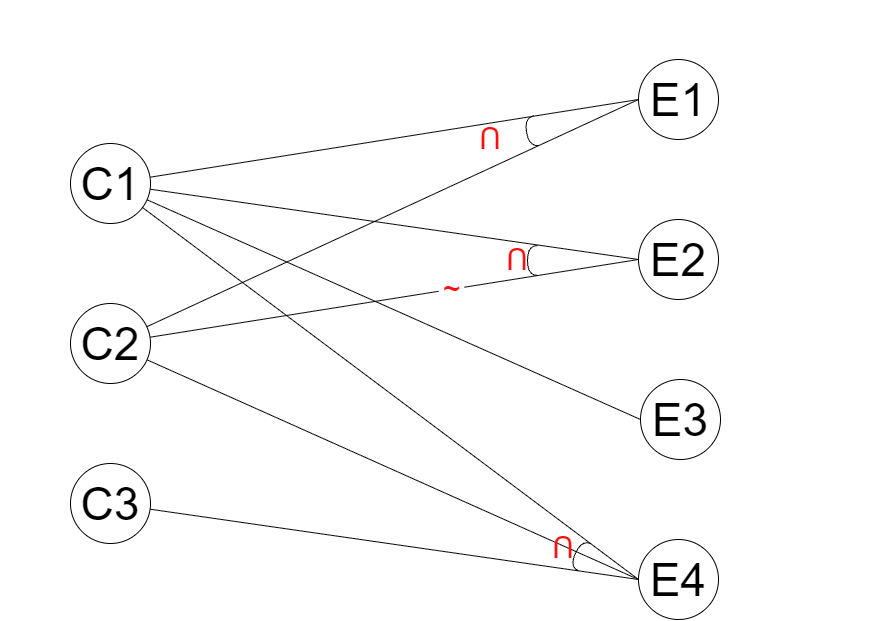
\includegraphics[width=0.82\textwidth,keepaspectratio]{CauseEffect_B5.png}
\caption{Đồ thị nhân -- quả chức năng Thích bài viết \& Bình luận (B5)}
\end{figure}

\noindent -- Bảng quyết định dẫn xuất (\texttt{R1}--\texttt{R4}):
\begin{table}[H]
\centering
\small
\begin{tabularx}{\textwidth}{|X|C{1.3cm}|C{1.3cm}|C{1.3cm}|C{1.3cm}|}
\hline
\rowcolor[RGB]{179, 205, 255}
\textbf{Conditions \& Actions} & \textbf{R1} & \textbf{R2} & \textbf{R3} & \textbf{R4} \tabularnewline
\hline
\multicolumn{5}{|l|}{\cellcolor{tableheader}\textbf{Conditions}} \\ \hline
C1: Người dùng nhấn nút trái tim? & N & Y & Y & Y \\ \hline
C2: Trạng thái trước khi nhấn là chưa thích (tim trắng)? & -- & Y & Y & N \\ \hline
C3: Người nhấn không phải tác giả bài viết? & -- & Y & N & -- \\ \hline
\multicolumn{5}{|l|}{\cellcolor{tableheader}\textbf{Actions}} \\ \hline
E1: Chuyển tim sang đỏ, tăng lượt thích $+1$ & & \textbf{X} & \textbf{X} & \\ \hline
E2: Chuyển tim về trắng, giảm lượt thích $-1$ & & & & \textbf{X} \\ \hline
E3: Đồng bộ số lượt thích tức thời đến người đang xem & & \textbf{X} & \textbf{X} & \textbf{X} \\ \hline
E4: Gửi thông báo tức thời cho tác giả & & \textbf{X} & & \\ \hline
\rowcolor{gray!15}
\textbf{Ánh xạ Test Case} & 103 & 107 & 108 & 105 \\ \hline
\end{tabularx}
\caption{Bảng quyết định dẫn xuất (\texttt{R1}--\texttt{R4}) từ Đồ thị nhân -- quả chức năng Thích bài viết (B5)}
\end{table}

\noindent\textbf{d. Bảng Test Cases chi tiết chức năng B5 (Thích bài viết \& Bình luận):}
\begingroup
\scriptsize
\setlength{\tabcolsep}{3pt}
\setlength{\LTpre}{4pt}
\setlength{\LTpost}{4pt}
\renewcommand{\arraystretch}{0.88}
\begin{longtable}{|C{0.8cm}|C{0.85cm}|C{0.95cm}|L{2.0cm}|L{3.0cm}|L{2.15cm}|L{2.6cm}|L{2.5cm}|C{0.85cm}|}
\hline
\rowcolor[RGB]{179, 205, 255}
\textbf{TC\#} & \textbf{BR\#} & \textbf{TR\#} & \textbf{TestCase} & \textbf{TestSteps} & \textbf{Test Data} & \textbf{Expected} & \textbf{Result} & \textbf{P/F} \tabularnewline
\hline
\endfirsthead
\hline
\rowcolor[RGB]{179, 205, 255}
\textbf{TC\#} & \textbf{BR\#} & \textbf{TR\#} & \textbf{TestCase} & \textbf{TestSteps} & \textbf{Test Data} & \textbf{Expected} & \textbf{Result} & \textbf{P/F} \tabularnewline
\hline
\endhead
\hline
\endfoot
\hline
\caption{Bảng Test Cases chức năng B5 -- Thích bài viết \& Bình luận (Cause--Effect Graph)}
\endlastfoot
\textbf{103} & B5 & T82 & Hiển thị nút trái tim kèm tổng số lượt thích (R1) & 1. Đăng nhập, mở Bảng tin\newline 2. Quan sát vùng tương tác dưới bài viết & Bài viết có 0 lượt thích & Hiển thị biểu tượng trái tim trắng kèm số lượng \texttt{0}. & Hiển thị đúng nút tim và bộ đếm. & \textcolor{blue}{\textbf{Pass}} \\ \hline
\textbf{105} & B5 & T84 & Nhấn bỏ thích bài viết khi tim đang đỏ (R4) & 1. Mở bài viết đã thích (tim đỏ, 1 thích)\newline 2. Nhấn lại vào nút trái tim & Bài viết PostId = 10 & Trái tim trở lại màu trắng và số lượng giảm về \texttt{0}. & Tim chuyển trắng, lượt thích giảm $-1$. & \textcolor{blue}{\textbf{Pass}} \\ \hline
\textbf{107} & B5 & T86 & Tác giả nhận thông báo khi người khác thích bài (R2) & 1. User2 thích bài viết của User1\newline 2. Kiểm tra chuông thông báo của User1 & Tác giả: User1\newline Người thích: User2 & Tim chuyển đỏ, lượt thích $+1$ và chuông User1 nhận thông báo thích bài. & User1 nhận thông báo tức thời. & \textcolor{blue}{\textbf{Pass}} \\ \hline
\textbf{108} & B5 & T86 & Tác giả tự thích bài viết của mình không tự thông báo (R3) & 1. User1 mở bài viết của chính mình\newline 2. User1 nhấn thích và kiểm tra chuông & Tác giả: User1\newline Người thích: User1 & Lượt thích tăng $+1$ nhưng không phát sinh thông báo tới chính User1. & Không gửi thông báo tự thích. & \textcolor{blue}{\textbf{Pass}} \\ \hline
\end{longtable}
\endgroup

% ----------------------------------------------------------
% 3.7 Pairwise
% ----------------------------------------------------------
\subsection{Kiểm thử cặp đôi (Pairwise / All-Pairs Testing)}

\subsubsection{Chức năng B4 -- Bảng tin \& Bài viết}

\noindent\textbf{a. Mô tả nghiệp vụ \& Yêu cầu kỹ thuật (TRD)}
\begin{itemize}[leftmargin=1.2cm, noitemsep]
    \item[\textbf{--}] \textbf{Mã BRD:} B4
    \item[\textbf{--}] \textbf{Tên chức năng:} Bảng tin \& Bài viết (News Feed \& Posts) -- Chức năng Đăng bài viết.
    \item[\textbf{--}] \textbf{Tóm tắt Requirement từ tài liệu hệ thống:}
    \begin{itemize}[leftmargin=0.8cm, label=$\ast$, noitemsep]
        \item \textbf{Quyền đăng bài:}
        \begin{itemize}[leftmargin=0.6cm, label=$\circ$, noitemsep]
            \item Người dùng phải đăng nhập thành công mới được truy cập chức năng đăng bài.
            \item Người dùng chưa đăng nhập không được phép thực hiện thao tác đăng bài viết.
        \end{itemize}
        \item \textbf{Nội dung bài viết:}
        \begin{itemize}[leftmargin=0.6cm, label=$\circ$, noitemsep]
            \item Nội dung (\texttt{Content}) không được để trống hoặc chỉ chứa khoảng trắng.
            \item Nội dung phải có độ dài từ 1 đến 5.000 ký tự.
            \item Nội dung dài phải tự động xuống dòng, không làm tràn khung hiển thị.
        \end{itemize}
        \item \textbf{Hình ảnh đính kèm:}
        \begin{itemize}[leftmargin=0.6cm, label=$\circ$, noitemsep]
            \item Hình ảnh là thành phần tùy chọn.
            \item Nếu có đính kèm, ảnh phải thuộc các định dạng JPG, JPEG, PNG, GIF hoặc WebP.
            \item Dung lượng ảnh không được vượt quá 5 MB.
            \item Hệ thống không cho phép đăng bài viết chỉ có hình ảnh mà không có nội dung văn bản.
        \end{itemize}
        \item \textbf{Xử lý đăng bài:}
        \begin{itemize}[leftmargin=0.6cm, label=$\circ$, noitemsep]
            \item Khi dữ liệu hợp lệ, hệ thống tạo và lưu bài viết mới.
            \item Sau khi đăng thành công, biểu mẫu được làm mới và bài viết xuất hiện trên Bảng tin.
            \item Bài viết mới được đồng bộ theo thời gian thực qua SignalR.
            \item Bạn bè của người đăng có thể nhận được thông báo theo quy định của hệ thống.
            \item Khi dữ liệu không hợp lệ, hệ thống từ chối đăng bài, hiển thị lỗi và không tạo bài viết mới.
        \end{itemize}
    \end{itemize}
\end{itemize}

\begin{table}[H]
\centering
\small
\begin{tabularx}{\textwidth}{|C{1.5cm}|X|}
\hline
\rowcolor[RGB]{179, 205, 255}
\textbf{T\#} & \textbf{Mô tả} \tabularnewline
\hline
\textbf{T64} & Người dùng phải đăng nhập mới có quyền đăng bài viết và xem Bảng tin. \\ \hline
\textbf{T65} & Không được đăng bài viết khi nội dung (\texttt{Content}) để trống hoặc chỉ chứa khoảng trắng. \\ \hline
\textbf{T66} & Nội dung bài viết phải có độ dài từ 1 đến tối đa 5.000 ký tự. \\ \hline
\textbf{T67} & Nội dung dài phải tự động xuống dòng, không làm tràn hoặc phá vỡ khung bài viết. \\ \hline
\textbf{T68} & Cho phép đính kèm ảnh JPG, JPEG, PNG, GIF hoặc WebP với dung lượng tối đa 5 MB. \\ \hline
\textbf{T69} & Từ chối tệp ảnh có dung lượng vượt quá 5 MB hoặc sai định dạng cho phép. \\ \hline
\textbf{T70} & Đăng bài thành công, biểu mẫu được làm mới và bài viết mới xuất hiện trên Bảng tin. \\ \hline
\textbf{T71} & Bài viết mới được đồng bộ theo thời gian thực qua SignalR. \\ \hline
\textbf{T72} & Bạn bè của người đăng nhận được thông báo khi có bài viết mới. \\ \hline
\end{tabularx}
\caption{Bảng TRD liên quan chức năng Đăng bài viết (\texttt{T64--T72})}
\end{table}

\noindent\textbf{b. Bảng xác định biến, giá trị \& Bảng kiểm thử cặp đôi (Pairwise)}

\begin{table}[H]
\centering
\small
\begin{tabularx}{\textwidth}{|L{4.2cm}|X|}
\hline
\rowcolor[RGB]{179, 205, 255}
\textbf{Yếu tố (Parameter)} & \textbf{Các giá trị kiểm thử (Values)} \tabularnewline
\hline
Trạng thái đăng nhập & Đã đăng nhập; Chưa đăng nhập \\ \hline
Nội dung bài viết & Trống; Chỉ có khoảng trắng; 1 ký tự; 100 ký tự; 4.999 ký tự; 5.000 ký tự; 5.001 ký tự \\ \hline
Đính kèm hình ảnh & Có; Không \\ \hline
Định dạng hình ảnh & JPG; JPEG; PNG; GIF; WebP; Không hỗ trợ; N/A (khi không có ảnh) \\ \hline
Dung lượng hình ảnh & Dưới 5 MB; Đúng 5 MB; Trên 5 MB; N/A (khi không có ảnh) \\ \hline
\end{tabularx}
\caption{Bảng xác định biến và giá trị kiểm thử cặp đôi cho chức năng Đăng bài (B4)}
\end{table}

\begin{longtable}{|C{1.2cm}|L{2.4cm}|L{2.6cm}|C{1.6cm}|L{2.5cm}|L{2.2cm}|C{2.0cm}|}
\hline
\rowcolor[RGB]{179, 205, 255}
\textbf{Mã ca} & \textbf{Đăng nhập} & \textbf{Nội dung} & \textbf{Kèm ảnh} & \textbf{Định dạng ảnh} & \textbf{Dung lượng} & \textbf{Ánh xạ TC} \tabularnewline
\hline
\endfirsthead
\hline
\rowcolor[RGB]{179, 205, 255}
\textbf{Mã ca} & \textbf{Đăng nhập} & \textbf{Nội dung} & \textbf{Kèm ảnh} & \textbf{Định dạng ảnh} & \textbf{Dung lượng} & \textbf{Ánh xạ TC} \tabularnewline
\hline
\endhead
\hline
\endfoot
\hline
\caption{Bảng 49 tổ hợp kiểm thử cặp đôi (Pairwise) chức năng Đăng bài viết (B4)}
\endlastfoot
PW01 & Đã đăng nhập & Trống & Có & JPEG & Dưới 5 MB & \texttt{TC 60} \\ \hline
PW02 & Đã đăng nhập & Chỉ khoảng trắng & Có & PNG & Bằng 5 MB & \texttt{TC 56.1} \\ \hline
PW03 & Đã đăng nhập & 100 ký tự & Không & N/A & N/A & \texttt{TC 59} \\ \hline
PW04 & Đã đăng nhập & 4999 ký tự & Có & JPG & Dưới 5 MB & \texttt{TC 67} \\ \hline
PW05 & Đã đăng nhập & 5000 ký tự & Có & WebP & Trên 5 MB & \texttt{TC 56.2} \\ \hline
PW06 & Đã đăng nhập & 5001 ký tự & Có & Không hỗ trợ & Bằng 5 MB & \texttt{TC 56.3} \\ \hline
PW07 & Chưa đăng nhập & Trống & Có & WebP & Dưới 5 MB & \texttt{TC 56.4} \\ \hline
PW08 & Chưa đăng nhập & Chỉ khoảng trắng & Có & JPG & Trên 5 MB & \texttt{TC 56.5} \\ \hline
PW09 & Chưa đăng nhập & 1 ký tự & Có & JPEG & Bằng 5 MB & \texttt{TC 56.6} \\ \hline
PW10 & Chưa đăng nhập & 100 ký tự & Có & GIF & Bằng 5 MB & \texttt{TC 56.7} \\ \hline
PW11 & Chưa đăng nhập & 4999 ký tự & Có & PNG & Bằng 5 MB & \texttt{TC 56.8} \\ \hline
PW12 & Chưa đăng nhập & 5001 ký tự & Không & N/A & N/A & \texttt{TC 56.9} \\ \hline
PW13 & Đã đăng nhập & Trống & Có & Không hỗ trợ & Trên 5 MB & \texttt{TC 56.10} \\ \hline
PW14 & Chưa đăng nhập & 100 ký tự & Có & JPEG & Trên 5 MB & \texttt{TC 56.11} \\ \hline
PW15 & Chưa đăng nhập & Trống & Có & JPG & Bằng 5 MB & \texttt{TC 56.12} \\ \hline
PW16 & Đã đăng nhập & Trống & Có & PNG & Dưới 5 MB & \texttt{TC 56.13} \\ \hline
PW17 & Đã đăng nhập & Trống & Có & GIF & Bằng 5 MB & \texttt{TC 56.14} \\ \hline
PW18 & Chưa đăng nhập & Trống & Không & N/A & N/A & \texttt{TC 56} \\ \hline
PW19 & Đã đăng nhập & Chỉ khoảng trắng & Có & JPEG & Dưới 5 MB & \texttt{TC 56.15} \\ \hline
PW20 & Đã đăng nhập & Chỉ khoảng trắng & Có & GIF & Bằng 5 MB & \texttt{TC 56.16} \\ \hline
PW21 & Đã đăng nhập & Chỉ khoảng trắng & Có & WebP & Trên 5 MB & \texttt{TC 56.17} \\ \hline
PW22 & Chưa đăng nhập & Chỉ khoảng trắng & Có & Không hỗ trợ & Dưới 5 MB & \texttt{TC 56.18} \\ \hline
PW23 & Chưa đăng nhập & Chỉ khoảng trắng & Không & N/A & N/A & \texttt{TC 56.19} \\ \hline
PW24 & Đã đăng nhập & 1 ký tự & Có & JPG & Trên 5 MB & \texttt{TC 56.20} \\ \hline
PW25 & Đã đăng nhập & 1 ký tự & Có & PNG & Dưới 5 MB & \texttt{TC 62} \\ \hline
PW26 & Chưa đăng nhập & 1 ký tự & Có & GIF & Dưới 5 MB & \texttt{TC 56.21} \\ \hline
PW27 & Chưa đăng nhập & 1 ký tự & Có & WebP & Bằng 5 MB & \texttt{TC 56.22} \\ \hline
PW28 & Đã đăng nhập & 1 ký tự & Có & Không hỗ trợ & Bằng 5 MB & \texttt{TC 74} \\ \hline
PW29 & Chưa đăng nhập & 1 ký tự & Không & N/A & N/A & \texttt{TC 56.23} \\ \hline
PW30 & Đã đăng nhập & 100 ký tự & Có & JPG & Bằng 5 MB & \texttt{TC 61} \\ \hline
PW31 & Chưa đăng nhập & 100 ký tự & Có & PNG & Trên 5 MB & \texttt{TC 56.24} \\ \hline
PW32 & Chưa đăng nhập & 100 ký tự & Có & WebP & Dưới 5 MB & \texttt{TC 56.25} \\ \hline
PW33 & Chưa đăng nhập & 100 ký tự & Có & Không hỗ trợ & Bằng 5 MB & \texttt{TC 56.26} \\ \hline
PW34 & Chưa đăng nhập & 4999 ký tự & Có & JPEG & Bằng 5 MB & \texttt{TC 56.27} \\ \hline
PW35 & Đã đăng nhập & 4999 ký tự & Có & GIF & Trên 5 MB & \texttt{TC 56.28} \\ \hline
PW36 & Đã đăng nhập & 4999 ký tự & Có & WebP & Trên 5 MB & \texttt{TC 56.29} \\ \hline
PW37 & Đã đăng nhập & 4999 ký tự & Có & Không hỗ trợ & Bằng 5 MB & \texttt{TC 56.30} \\ \hline
PW38 & Chưa đăng nhập & 4999 ký tự & Không & N/A & N/A & \texttt{TC 56.31} \\ \hline
PW39 & Chưa đăng nhập & 5000 ký tự & Có & JPEG & Dưới 5 MB & \texttt{TC 56.32} \\ \hline
PW40 & Đã đăng nhập & 5000 ký tự & Có & JPG & Trên 5 MB & \texttt{TC 73} \\ \hline
PW41 & Chưa đăng nhập & 5000 ký tự & Có & PNG & Dưới 5 MB & \texttt{TC 56.33} \\ \hline
PW42 & Đã đăng nhập & 5000 ký tự & Có & GIF & Dưới 5 MB & \texttt{TC 70} \\ \hline
PW43 & Đã đăng nhập & 5000 ký tự & Có & Không hỗ trợ & Bằng 5 MB & \texttt{TC 56.34} \\ \hline
PW44 & Đã đăng nhập & 5000 ký tự & Không & N/A & N/A & \texttt{TC 63} \\ \hline
PW45 & Đã đăng nhập & 5001 ký tự & Có & JPEG & Dưới 5 MB & \texttt{TC 64} \\ \hline
PW46 & Chưa đăng nhập & 5001 ký tự & Có & JPG & Trên 5 MB & \texttt{TC 56.35} \\ \hline
PW47 & Đã đăng nhập & 5001 ký tự & Có & PNG & Bằng 5 MB & \texttt{TC 56.36} \\ \hline
PW48 & Chưa đăng nhập & 5001 ký tự & Có & GIF & Bằng 5 MB & \texttt{TC 56.37} \\ \hline
PW49 & Đã đăng nhập & 5001 ký tự & Có & WebP & Dưới 5 MB & \texttt{TC 56.38} \\ \hline
\end{longtable}

\noindent\textbf{Bảng Test Cases chi tiết chức năng B4 (Đăng bài trên Bảng tin -- Pairwise):}
\begingroup
\scriptsize
\setlength{\tabcolsep}{3pt}
\begin{longtable}{|C{0.85cm}|C{0.7cm}|C{0.95cm}|L{2.0cm}|L{3.0cm}|L{2.2cm}|L{2.6cm}|L{2.5cm}|C{0.85cm}|}
\hline
\rowcolor[RGB]{179, 205, 255}
\textbf{TC\#} & \textbf{BR\#} & \textbf{TR\#} & \textbf{TestCase} & \textbf{TestSteps} & \textbf{Test Data} & \textbf{Expected} & \textbf{Result} & \textbf{P/F} \tabularnewline
\hline
\endfirsthead
\hline
\rowcolor[RGB]{179, 205, 255}
\textbf{TC\#} & \textbf{BR\#} & \textbf{TR\#} & \textbf{TestCase} & \textbf{TestSteps} & \textbf{Test Data} & \textbf{Expected} & \textbf{Result} & \textbf{P/F} \tabularnewline
\hline
\endhead
\hline
\endfoot
\hline
\caption{Bảng Test Cases chức năng B4 -- Đăng bài trên Bảng tin (Pairwise)}
\endlastfoot
\textbf{56} & B4 & T64 & Đăng bài khi chưa đăng nhập (PW18) & 1. Chưa đăng nhập\newline 2. Nhập trực tiếp URL trang bảng tin & URL: /home\newline ND: (trống), không ảnh & Chặn truy cập bảng tin và giữ/chuyển về trang đăng nhập. & Giữ người dùng tại trang đăng nhập. & \textcolor{blue}{\textbf{Pass}} \\ \hline
\textbf{56.1} & B4 & T65 & Chặn đăng bài nội dung chỉ khoảng trắng kèm ảnh PNG (PW02) & 1. Đăng nhập\newline 2. Nhập ND chỉ khoảng trắng, chọn PNG (Bằng 5 MB), bấm Đăng & ND: Chỉ khoảng trắng\newline Ảnh: PNG (Bằng 5 MB) & Chặn gửi do thiếu nội dung văn bản hoặc lỗi tệp ảnh. & Chặn gửi và hiển thị thông báo lỗi hợp lệ. & \textcolor{blue}{\textbf{Pass}} \\ \hline
\textbf{56.2} & B4 & T69 & Chặn đăng bài 5000 ký tự kèm ảnh WebP vượt 5MB (PW05) & 1. Đăng nhập\newline 2. Nhập ND 5000 ký tự, đính kèm WebP (>5MB), bấm Đăng & ND: 5000 ký tự\newline Ảnh: WebP (6.2MB) & Từ chối đăng, báo lỗi kích thước ảnh vượt quá 5MB. & Chặn đăng và hiển thị đúng cảnh báo vượt 5MB. & \textcolor{blue}{\textbf{Pass}} \\ \hline
\textbf{56.3} & B4 & T69 & Chặn đăng bài 5001 ký tự với tệp sai định dạng (PW06) & 1. Đăng nhập\newline 2. Nhập ND 5001 ký tự, đính kèm file .pdf (Bằng 5 MB), bấm Đăng & ND: 5001 ký tự\newline File: doc.pdf (Bằng 5 MB) & Từ chối đăng, báo lỗi định dạng ảnh không được hỗ trợ. & Chặn đăng và hiển thị đúng cảnh báo định dạng. & \textcolor{blue}{\textbf{Pass}} \\ \hline
\textbf{56.4} & B4 & T64 & Chặn đăng bài khi chưa đăng nhập (PW07) & 1. Chưa đăng nhập\newline 2. Gửi yêu cầu đăng bài (Trống, WebP) & Chưa đăng nhập\newline ND: Trống\newline Ảnh: WebP (Dưới 5 MB) & Từ chối HTTP 401 Unauthorized hoặc chuyển hướng về trang đăng nhập. & Chặn truy cập chưa đăng nhập và chuyển về \texttt{/login}. & \textcolor{blue}{\textbf{Pass}} \\ \hline
\textbf{56.5} & B4 & T64 & Chặn đăng bài khi chưa đăng nhập (PW08) & 1. Chưa đăng nhập\newline 2. Gửi yêu cầu đăng bài (Chỉ khoảng trắng, JPG) & Chưa đăng nhập\newline ND: Chỉ khoảng trắng\newline Ảnh: JPG (Trên 5 MB) & Từ chối HTTP 401 Unauthorized hoặc chuyển hướng về trang đăng nhập. & Chặn truy cập chưa đăng nhập và chuyển về \texttt{/login}. & \textcolor{blue}{\textbf{Pass}} \\ \hline
\textbf{56.6} & B4 & T64 & Chặn đăng bài khi chưa đăng nhập (PW09) & 1. Chưa đăng nhập\newline 2. Gửi yêu cầu đăng bài (1 ký tự, JPEG) & Chưa đăng nhập\newline ND: 1 ký tự\newline Ảnh: JPEG (Bằng 5 MB) & Từ chối HTTP 401 Unauthorized hoặc chuyển hướng về trang đăng nhập. & Chặn truy cập chưa đăng nhập và chuyển về \texttt{/login}. & \textcolor{blue}{\textbf{Pass}} \\ \hline
\textbf{56.7} & B4 & T64 & Chặn đăng bài khi chưa đăng nhập (PW10) & 1. Chưa đăng nhập\newline 2. Gửi yêu cầu đăng bài (100 ký tự, GIF) & Chưa đăng nhập\newline ND: 100 ký tự\newline Ảnh: GIF (Bằng 5 MB) & Từ chối HTTP 401 Unauthorized hoặc chuyển hướng về trang đăng nhập. & Chặn truy cập chưa đăng nhập và chuyển về \texttt{/login}. & \textcolor{blue}{\textbf{Pass}} \\ \hline
\textbf{56.8} & B4 & T64 & Chặn đăng bài khi chưa đăng nhập (PW11) & 1. Chưa đăng nhập\newline 2. Gửi yêu cầu đăng bài (4999 ký tự, PNG) & Chưa đăng nhập\newline ND: 4999 ký tự\newline Ảnh: PNG (Bằng 5 MB) & Từ chối HTTP 401 Unauthorized hoặc chuyển hướng về trang đăng nhập. & Chặn truy cập chưa đăng nhập và chuyển về \texttt{/login}. & \textcolor{blue}{\textbf{Pass}} \\ \hline
\textbf{56.9} & B4 & T64 & Chặn đăng bài khi chưa đăng nhập (PW12) & 1. Chưa đăng nhập\newline 2. Gửi yêu cầu đăng bài (5001 ký tự, N/A) & Chưa đăng nhập\newline ND: 5001 ký tự\newline Ảnh: N/A (N/A) & Từ chối HTTP 401 Unauthorized hoặc chuyển hướng về trang đăng nhập. & Chặn truy cập chưa đăng nhập và chuyển về \texttt{/login}. & \textcolor{blue}{\textbf{Pass}} \\ \hline
\textbf{56.10} & B4 & T65, T69 & Chặn đăng bài nội dung trống kèm ảnh Không hỗ trợ (PW13) & 1. Đăng nhập\newline 2. Nhập ND trống, chọn Không hỗ trợ (Trên 5 MB), bấm Đăng & ND: Trống\newline Ảnh: Không hỗ trợ (Trên 5 MB) & Chặn gửi do thiếu nội dung văn bản hoặc lỗi tệp ảnh. & Chặn gửi và hiển thị thông báo lỗi hợp lệ. & \textcolor{blue}{\textbf{Pass}} \\ \hline
\textbf{56.11} & B4 & T64 & Chặn đăng bài khi chưa đăng nhập (PW14) & 1. Chưa đăng nhập\newline 2. Gửi yêu cầu đăng bài (100 ký tự, JPEG) & Chưa đăng nhập\newline ND: 100 ký tự\newline Ảnh: JPEG (Trên 5 MB) & Từ chối HTTP 401 Unauthorized hoặc chuyển hướng về trang đăng nhập. & Chặn truy cập chưa đăng nhập và chuyển về \texttt{/login}. & \textcolor{blue}{\textbf{Pass}} \\ \hline
\textbf{56.12} & B4 & T64 & Chặn đăng bài khi chưa đăng nhập (PW15) & 1. Chưa đăng nhập\newline 2. Gửi yêu cầu đăng bài (Trống, JPG) & Chưa đăng nhập\newline ND: Trống\newline Ảnh: JPG (Bằng 5 MB) & Từ chối HTTP 401 Unauthorized hoặc chuyển hướng về trang đăng nhập. & Chặn truy cập chưa đăng nhập và chuyển về \texttt{/login}. & \textcolor{blue}{\textbf{Pass}} \\ \hline
\textbf{56.13} & B4 & T65 & Chặn đăng bài nội dung trống kèm ảnh PNG (PW16) & 1. Đăng nhập\newline 2. Nhập ND trống, chọn PNG (Dưới 5 MB), bấm Đăng & ND: Trống\newline Ảnh: PNG (Dưới 5 MB) & Chặn gửi do thiếu nội dung văn bản hoặc lỗi tệp ảnh. & Chặn gửi và hiển thị thông báo lỗi hợp lệ. & \textcolor{blue}{\textbf{Pass}} \\ \hline
\textbf{56.14} & B4 & T65 & Chặn đăng bài nội dung trống kèm ảnh GIF (PW17) & 1. Đăng nhập\newline 2. Nhập ND trống, chọn GIF (Bằng 5 MB), bấm Đăng & ND: Trống\newline Ảnh: GIF (Bằng 5 MB) & Chặn gửi do thiếu nội dung văn bản hoặc lỗi tệp ảnh. & Chặn gửi và hiển thị thông báo lỗi hợp lệ. & \textcolor{blue}{\textbf{Pass}} \\ \hline
\textbf{56.15} & B4 & T65 & Chặn đăng bài nội dung chỉ khoảng trắng kèm ảnh JPEG (PW19) & 1. Đăng nhập\newline 2. Nhập ND chỉ khoảng trắng, chọn JPEG (Dưới 5 MB), bấm Đăng & ND: Chỉ khoảng trắng\newline Ảnh: JPEG (Dưới 5 MB) & Chặn gửi do thiếu nội dung văn bản hoặc lỗi tệp ảnh. & Chặn gửi và hiển thị thông báo lỗi hợp lệ. & \textcolor{blue}{\textbf{Pass}} \\ \hline
\textbf{56.16} & B4 & T65 & Chặn đăng bài nội dung chỉ khoảng trắng kèm ảnh GIF (PW20) & 1. Đăng nhập\newline 2. Nhập ND chỉ khoảng trắng, chọn GIF (Bằng 5 MB), bấm Đăng & ND: Chỉ khoảng trắng\newline Ảnh: GIF (Bằng 5 MB) & Chặn gửi do thiếu nội dung văn bản hoặc lỗi tệp ảnh. & Chặn gửi và hiển thị thông báo lỗi hợp lệ. & \textcolor{blue}{\textbf{Pass}} \\ \hline
\textbf{56.17} & B4 & T65, T69 & Chặn đăng bài nội dung chỉ khoảng trắng kèm ảnh WebP (PW21) & 1. Đăng nhập\newline 2. Nhập ND chỉ khoảng trắng, chọn WebP (Trên 5 MB), bấm Đăng & ND: Chỉ khoảng trắng\newline Ảnh: WebP (Trên 5 MB) & Chặn gửi do thiếu nội dung văn bản hoặc lỗi tệp ảnh. & Chặn gửi và hiển thị thông báo lỗi hợp lệ. & \textcolor{blue}{\textbf{Pass}} \\ \hline
\textbf{56.18} & B4 & T64 & Chặn đăng bài khi chưa đăng nhập (PW22) & 1. Chưa đăng nhập\newline 2. Gửi yêu cầu đăng bài (Chỉ khoảng trắng, Không hỗ trợ) & Chưa đăng nhập\newline ND: Chỉ khoảng trắng\newline Ảnh: Không hỗ trợ (Dưới 5 MB) & Từ chối HTTP 401 Unauthorized hoặc chuyển hướng về trang đăng nhập. & Chặn truy cập chưa đăng nhập và chuyển về \texttt{/login}. & \textcolor{blue}{\textbf{Pass}} \\ \hline
\textbf{56.19} & B4 & T64 & Chặn đăng bài khi chưa đăng nhập (PW23) & 1. Chưa đăng nhập\newline 2. Gửi yêu cầu đăng bài (Chỉ khoảng trắng, N/A) & Chưa đăng nhập\newline ND: Chỉ khoảng trắng\newline Ảnh: N/A (N/A) & Từ chối HTTP 401 Unauthorized hoặc chuyển hướng về trang đăng nhập. & Chặn truy cập chưa đăng nhập và chuyển về \texttt{/login}. & \textcolor{blue}{\textbf{Pass}} \\ \hline
\textbf{56.20} & B4 & T69 & Chặn đăng bài 1 ký tự kèm ảnh JPG vượt 5MB (PW24) & 1. Đăng nhập\newline 2. Nhập ND 1 ký tự, đính kèm JPG (>5MB), bấm Đăng & ND: 1 ký tự\newline Ảnh: JPG (6.2MB) & Từ chối đăng, báo lỗi kích thước ảnh vượt quá 5MB. & Chặn đăng và hiển thị đúng cảnh báo vượt 5MB. & \textcolor{blue}{\textbf{Pass}} \\ \hline
\textbf{56.21} & B4 & T64 & Chặn đăng bài khi chưa đăng nhập (PW26) & 1. Chưa đăng nhập\newline 2. Gửi yêu cầu đăng bài (1 ký tự, GIF) & Chưa đăng nhập\newline ND: 1 ký tự\newline Ảnh: GIF (Dưới 5 MB) & Từ chối HTTP 401 Unauthorized hoặc chuyển hướng về trang đăng nhập. & Chặn truy cập chưa đăng nhập và chuyển về \texttt{/login}. & \textcolor{blue}{\textbf{Pass}} \\ \hline
\textbf{56.22} & B4 & T64 & Chặn đăng bài khi chưa đăng nhập (PW27) & 1. Chưa đăng nhập\newline 2. Gửi yêu cầu đăng bài (1 ký tự, WebP) & Chưa đăng nhập\newline ND: 1 ký tự\newline Ảnh: WebP (Bằng 5 MB) & Từ chối HTTP 401 Unauthorized hoặc chuyển hướng về trang đăng nhập. & Chặn truy cập chưa đăng nhập và chuyển về \texttt{/login}. & \textcolor{blue}{\textbf{Pass}} \\ \hline
\textbf{56.23} & B4 & T64 & Chặn đăng bài khi chưa đăng nhập (PW29) & 1. Chưa đăng nhập\newline 2. Gửi yêu cầu đăng bài (1 ký tự, N/A) & Chưa đăng nhập\newline ND: 1 ký tự\newline Ảnh: N/A (N/A) & Từ chối HTTP 401 Unauthorized hoặc chuyển hướng về trang đăng nhập. & Chặn truy cập chưa đăng nhập và chuyển về \texttt{/login}. & \textcolor{blue}{\textbf{Pass}} \\ \hline
\textbf{56.24} & B4 & T64 & Chặn đăng bài khi chưa đăng nhập (PW31) & 1. Chưa đăng nhập\newline 2. Gửi yêu cầu đăng bài (100 ký tự, PNG) & Chưa đăng nhập\newline ND: 100 ký tự\newline Ảnh: PNG (Trên 5 MB) & Từ chối HTTP 401 Unauthorized hoặc chuyển hướng về trang đăng nhập. & Chặn truy cập chưa đăng nhập và chuyển về \texttt{/login}. & \textcolor{blue}{\textbf{Pass}} \\ \hline
\textbf{56.25} & B4 & T64 & Chặn đăng bài khi chưa đăng nhập (PW32) & 1. Chưa đăng nhập\newline 2. Gửi yêu cầu đăng bài (100 ký tự, WebP) & Chưa đăng nhập\newline ND: 100 ký tự\newline Ảnh: WebP (Dưới 5 MB) & Từ chối HTTP 401 Unauthorized hoặc chuyển hướng về trang đăng nhập. & Chặn truy cập chưa đăng nhập và chuyển về \texttt{/login}. & \textcolor{blue}{\textbf{Pass}} \\ \hline
\textbf{56.26} & B4 & T64 & Chặn đăng bài khi chưa đăng nhập (PW33) & 1. Chưa đăng nhập\newline 2. Gửi yêu cầu đăng bài (100 ký tự, Không hỗ trợ) & Chưa đăng nhập\newline ND: 100 ký tự\newline Ảnh: Không hỗ trợ (Bằng 5 MB) & Từ chối HTTP 401 Unauthorized hoặc chuyển hướng về trang đăng nhập. & Chặn truy cập chưa đăng nhập và chuyển về \texttt{/login}. & \textcolor{blue}{\textbf{Pass}} \\ \hline
\textbf{56.27} & B4 & T64 & Chặn đăng bài khi chưa đăng nhập (PW34) & 1. Chưa đăng nhập\newline 2. Gửi yêu cầu đăng bài (4999 ký tự, JPEG) & Chưa đăng nhập\newline ND: 4999 ký tự\newline Ảnh: JPEG (Bằng 5 MB) & Từ chối HTTP 401 Unauthorized hoặc chuyển hướng về trang đăng nhập. & Chặn truy cập chưa đăng nhập và chuyển về \texttt{/login}. & \textcolor{blue}{\textbf{Pass}} \\ \hline
\textbf{56.28} & B4 & T69 & Chặn đăng bài 4999 ký tự kèm ảnh GIF vượt 5MB (PW35) & 1. Đăng nhập\newline 2. Nhập ND 4999 ký tự, đính kèm GIF (>5MB), bấm Đăng & ND: 4999 ký tự\newline Ảnh: GIF (6.2MB) & Từ chối đăng, báo lỗi kích thước ảnh vượt quá 5MB. & Chặn đăng và hiển thị đúng cảnh báo vượt 5MB. & \textcolor{blue}{\textbf{Pass}} \\ \hline
\textbf{56.29} & B4 & T69 & Chặn đăng bài 4999 ký tự kèm ảnh WebP vượt 5MB (PW36) & 1. Đăng nhập\newline 2. Nhập ND 4999 ký tự, đính kèm WebP (>5MB), bấm Đăng & ND: 4999 ký tự\newline Ảnh: WebP (6.2MB) & Từ chối đăng, báo lỗi kích thước ảnh vượt quá 5MB. & Chặn đăng và hiển thị đúng cảnh báo vượt 5MB. & \textcolor{blue}{\textbf{Pass}} \\ \hline
\textbf{56.30} & B4 & T69 & Chặn đăng bài 4999 ký tự với tệp sai định dạng (PW37) & 1. Đăng nhập\newline 2. Nhập ND 4999 ký tự, đính kèm file .pdf (Bằng 5 MB), bấm Đăng & ND: 4999 ký tự\newline File: doc.pdf (Bằng 5 MB) & Từ chối đăng, báo lỗi định dạng ảnh không được hỗ trợ. & Chặn đăng và hiển thị đúng cảnh báo định dạng. & \textcolor{blue}{\textbf{Pass}} \\ \hline
\textbf{56.31} & B4 & T64 & Chặn đăng bài khi chưa đăng nhập (PW38) & 1. Chưa đăng nhập\newline 2. Gửi yêu cầu đăng bài (4999 ký tự, N/A) & Chưa đăng nhập\newline ND: 4999 ký tự\newline Ảnh: N/A (N/A) & Từ chối HTTP 401 Unauthorized hoặc chuyển hướng về trang đăng nhập. & Chặn truy cập chưa đăng nhập và chuyển về \texttt{/login}. & \textcolor{blue}{\textbf{Pass}} \\ \hline
\textbf{56.32} & B4 & T64 & Chặn đăng bài khi chưa đăng nhập (PW39) & 1. Chưa đăng nhập\newline 2. Gửi yêu cầu đăng bài (5000 ký tự, JPEG) & Chưa đăng nhập\newline ND: 5000 ký tự\newline Ảnh: JPEG (Dưới 5 MB) & Từ chối HTTP 401 Unauthorized hoặc chuyển hướng về trang đăng nhập. & Chặn truy cập chưa đăng nhập và chuyển về \texttt{/login}. & \textcolor{blue}{\textbf{Pass}} \\ \hline
\textbf{56.33} & B4 & T64 & Chặn đăng bài khi chưa đăng nhập (PW41) & 1. Chưa đăng nhập\newline 2. Gửi yêu cầu đăng bài (5000 ký tự, PNG) & Chưa đăng nhập\newline ND: 5000 ký tự\newline Ảnh: PNG (Dưới 5 MB) & Từ chối HTTP 401 Unauthorized hoặc chuyển hướng về trang đăng nhập. & Chặn truy cập chưa đăng nhập và chuyển về \texttt{/login}. & \textcolor{blue}{\textbf{Pass}} \\ \hline
\textbf{56.34} & B4 & T69 & Chặn đăng bài 5000 ký tự với tệp sai định dạng (PW43) & 1. Đăng nhập\newline 2. Nhập ND 5000 ký tự, đính kèm file .pdf (Bằng 5 MB), bấm Đăng & ND: 5000 ký tự\newline File: doc.pdf (Bằng 5 MB) & Từ chối đăng, báo lỗi định dạng ảnh không được hỗ trợ. & Chặn đăng và hiển thị đúng cảnh báo định dạng. & \textcolor{blue}{\textbf{Pass}} \\ \hline
\textbf{56.35} & B4 & T64 & Chặn đăng bài khi chưa đăng nhập (PW46) & 1. Chưa đăng nhập\newline 2. Gửi yêu cầu đăng bài (5001 ký tự, JPG) & Chưa đăng nhập\newline ND: 5001 ký tự\newline Ảnh: JPG (Trên 5 MB) & Từ chối HTTP 401 Unauthorized hoặc chuyển hướng về trang đăng nhập. & Chặn truy cập chưa đăng nhập và chuyển về \texttt{/login}. & \textcolor{blue}{\textbf{Pass}} \\ \hline
\textbf{56.36} & B4 & T66 & Kiểm tra ràng buộc 5001 ký tự kèm PNG (PW47) & 1. Đăng nhập\newline 2. Gửi POST tạo bài 5001 ký tự kèm PNG (Bằng 5 MB) & ND: 5001 kt\newline Ảnh: PNG (Bằng 5 MB) & Hệ thống kiểm tra giới hạn tối đa 5000 ký tự và trả lỗi hợp lệ. & API từ chối vượt 5000 ký tự theo đúng ràng buộc T66. & \textcolor{blue}{\textbf{Pass}} \\ \hline
\textbf{56.37} & B4 & T64 & Chặn đăng bài khi chưa đăng nhập (PW48) & 1. Chưa đăng nhập\newline 2. Gửi yêu cầu đăng bài (5001 ký tự, GIF) & Chưa đăng nhập\newline ND: 5001 ký tự\newline Ảnh: GIF (Bằng 5 MB) & Từ chối HTTP 401 Unauthorized hoặc chuyển hướng về trang đăng nhập. & Chặn truy cập chưa đăng nhập và chuyển về \texttt{/login}. & \textcolor{blue}{\textbf{Pass}} \\ \hline
\textbf{56.38} & B4 & T66 & Kiểm tra ràng buộc 5001 ký tự kèm WebP (PW49) & 1. Đăng nhập\newline 2. Gửi POST tạo bài 5001 ký tự kèm WebP (Dưới 5 MB) & ND: 5001 kt\newline Ảnh: WebP (Dưới 5 MB) & Hệ thống kiểm tra giới hạn tối đa 5000 ký tự và trả lỗi hợp lệ. & API từ chối vượt 5000 ký tự theo đúng ràng buộc T66. & \textcolor{blue}{\textbf{Pass}} \\ \hline
\textbf{59} & B4 & T65 & Đăng bài chỉ có nội dung văn bản (PW03) & 1. Đăng nhập\newline 2. Nhập 100 ký tự hợp lệ, không chọn ảnh, bấm Đăng & ND: 100 ký tự\newline Ảnh: không & Đăng bài thành công, hiển thị bài ở đầu trang. & Đăng thành công ở đầu trang. & \textcolor{blue}{\textbf{Pass}} \\ \hline
\textbf{60} & B4 & T65 & Đăng bài chỉ có hình ảnh (trống văn bản) (PW01) & 1. Đăng nhập\newline 2. Để trống chữ, chọn ảnh JPEG (<5MB), bấm Đăng & ND: (trống)\newline Ảnh: pic.jpg (1.2MB) & Chặn gửi khi thiếu nội dung văn bản. & Chặn gửi, báo lỗi ``Validation failed''. & \textcolor{blue}{\textbf{Pass}} \\ \hline
\textbf{61} & B4 & T65, T68 & Đăng bài có cả hình ảnh và nội dung (PW30) & 1. Đăng nhập, nhập 100 ký tự\newline 2. Chọn pic.jpg (5MB), bấm Đăng & ND: 100 kt\newline Ảnh: pic.jpg (5MB) & Đăng bài thành công, hiển thị cả chữ và ảnh ở đầu trang. & Đăng thành công ở đầu trang. & \textcolor{blue}{\textbf{Pass}} \\ \hline
\textbf{62} & B4 & T66, T68 & Đăng bài độ dài tối thiểu 1 ký tự kèm PNG (PW25) & 1. Đăng nhập\newline 2. Nhập 1 ký tự ``D'', kèm ảnh PNG (<5MB), bấm Đăng & ND: ``D''\newline Ảnh: pic.png (1.2MB) & Đăng bài thành công, xuất hiện đầu bảng tin. & Đăng thành công. & \textcolor{blue}{\textbf{Pass}} \\ \hline
\textbf{63} & B4 & T66 & Đăng bài với nội dung đúng 5000 ký tự (PW44) & 1. Đăng nhập\newline 2. Nhập đúng 5000 ký tự, không ảnh, bấm Đăng & ND: 5000 ký tự\newline Ảnh: không & Đăng bài thành công, xuất hiện đầu bảng tin. & Đăng thành công. & \textcolor{blue}{\textbf{Pass}} \\ \hline
\textbf{64} & B4 & T66 & Đăng bài với nội dung lớn hơn 5000 ký tự (PW45) & 1. Đăng nhập\newline 2. Nhập 5001 ký tự, kèm JPEG (<5MB), bấm Đăng & ND: 5001 kt\newline Ảnh: pic.jpeg (1.2MB) & Chặn đăng, báo lỗi vượt quá giới hạn 5000 ký tự. & Vẫn đăng thành công bài > 5000 ký tự trên UI v1.0 (Defect \#1). & \textcolor{red}{\textbf{Fail}} \\ \hline
\textbf{67} & B4 & T68 & Đăng bài kèm tệp ảnh JPG hợp lệ (PW04) & 1. Nhập 4999 ký tự\newline 2. Đính kèm pic.jpg (<5MB), nhấn Đăng & ND: 4999 kt\newline Ảnh: pic.jpg (1.7MB) & Đăng bài thành công, hiển thị đầy đủ nội dung và ảnh. & Đăng thành công. & \textcolor{blue}{\textbf{Pass}} \\ \hline
\textbf{70} & B4 & T68 & Đăng bài kèm tệp ảnh GIF hợp lệ (PW42) & 1. Nhập 5000 ký tự\newline 2. Đính kèm pic.gif (<5MB), nhấn Đăng & ND: 5000 kt\newline Ảnh: pic.gif (1.2MB) & Đăng thành công; ảnh GIF hiển thị và chuyển động bình thường. & Ảnh GIF bị lỗi chuyển động trên bảng tin (Defect \#3). & \textcolor{red}{\textbf{Fail}} \\ \hline
\textbf{73} & B4 & T69 & Đăng bài kèm ảnh vượt 5MB (PW40) & 1. Nhập 5000 ký tự\newline 2. Đính kèm pic.jpg (>5MB), nhấn Đăng & ND: 5000 kt\newline Ảnh: pic.jpg (8.5MB) & Từ chối đăng, báo lỗi ``Kích thước hình ảnh không được vượt quá 5MB''. & Chặn đăng và báo lỗi đúng. & \textcolor{blue}{\textbf{Pass}} \\ \hline
\textbf{74} & B4 & T69 & Đăng bài kèm tệp sai định dạng (PW28) & 1. Nhập 1 ký tự ``D''\newline 2. Đính kèm tệp không hỗ trợ (5MB), nhấn Đăng & ND: ``D''\newline File: text.pdf (5MB) & Từ chối đăng, báo lỗi ``Chỉ hỗ trợ các định dạng: JPEG, PNG, GIF, WebP''. & Chặn đăng và báo lỗi đúng. & \textcolor{blue}{\textbf{Pass}} \\ \hline
\end{longtable}
\endgroup

\subsubsection{Chức năng B12 -- Tìm kiếm toàn hệ thống}

\noindent\textbf{a. Mô tả nghiệp vụ \& Yêu cầu kỹ thuật (TRD)}
\begin{itemize}[leftmargin=1.2cm, noitemsep]
    \item[\textbf{--}] \textbf{Mã BRD:} B12
    \item[\textbf{--}] \textbf{Tên chức năng:} Tìm kiếm toàn hệ thống (Search \& Discovery) -- Tìm kiếm người dùng, bài viết, nhóm cộng đồng và lọc cuộc trò chuyện tin nhắn.
    \item[\textbf{--}] \textbf{Tóm tắt Requirement từ tài liệu hệ thống:}
    \begin{itemize}[leftmargin=0.8cm, label=$\ast$, noitemsep]
        \item \textbf{Tìm kiếm trên Header \& Bảng tin:} Hỗ trợ tìm kiếm người dùng theo tên/username từ thanh tiêu đề (Header) và tìm kiếm bài viết trên Bảng tin chung theo từ khóa nội dung hoặc tên tác giả.
        \item \textbf{Tìm kiếm trong Nhóm cộng đồng:} Hỗ trợ lọc danh sách nhóm theo tên trên trang \texttt{/groups} và tìm kiếm nhanh bài viết trong phạm vi một nhóm cụ thể.
        \item \textbf{Lọc danh sách Tin nhắn:} Hỗ trợ lọc tức thì danh sách cuộc trò chuyện theo tên bạn bè hoặc tên nhóm chat.
        \item \textbf{Phản hồi giao diện:} Hỗ trợ lọc tức thì khi nhập liệu hoặc khi nhấn Enter; xử lý an toàn các từ khóa trống, ký tự đặc biệt hoặc không có kết quả phù hợp.
    \end{itemize}
\end{itemize}

\begin{table}[H]
\centering
\small
\begin{tabularx}{\textwidth}{|C{1.5cm}|X|}
\hline
\rowcolor[RGB]{179, 205, 255}
\textbf{T\#} & \textbf{Mô tả} \tabularnewline
\hline
\textbf{T142} & Tìm kiếm người dùng từ thanh tìm kiếm Header theo tên hoặc username. \\ \hline
\textbf{T143} & Tìm kiếm bài viết trên Bảng tin chung (Feed) theo từ khóa nội dung hoặc tên tác giả. \\ \hline
\textbf{T144} & Tìm kiếm và lọc nhóm theo tên trên trang danh sách Nhóm cộng đồng (\texttt{/groups}). \\ \hline
\textbf{T145} & Tìm kiếm nhanh bài viết trong phạm vi một nhóm cụ thể. \\ \hline
\textbf{T146} & Lọc danh sách cuộc trò chuyện tin nhắn theo tên bạn bè hoặc nhóm chat. \\ \hline
\end{tabularx}
\caption{Bảng TRD liên quan chức năng Tìm kiếm toàn hệ thống (\texttt{T142--T146})}
\end{table}

\noindent\textbf{b. Bảng xác định biến, giá trị \& Bảng kiểm thử cặp đôi (Pairwise)}

Từ đặc tả chức năng B12, xác định 4 biến đầu vào với kích thước $4^2\,2^2$ ($4 \times 4 \times 2 \times 2 = 64$ tổ hợp toàn phần). Áp dụng kỹ thuật cặp đôi theo ma trận trực giao $L_{16}(4^2\,2^2)$ (từ tệp \texttt{B12.xlsx}) rút gọn xuống còn \textbf{16 ca kiểm thử} (\texttt{PW01}--\texttt{PW16}) mà vẫn phủ 100\% mọi cặp giá trị giữa 2 biến bất kỳ:

\begin{table}[H]
\centering
\small
\begin{tabularx}{\textwidth}{|L{4.5cm}|X|}
\hline
\rowcolor[RGB]{179, 205, 255}
\textbf{Yếu tố (Parameter)} & \textbf{Các giá trị kiểm thử (Values)} \tabularnewline
\hline
Phạm vi tìm kiếm & Người dùng; Bài viết; Nhóm; Tin nhắn \\ \hline
Loại từ khóa & Hợp lệ; Không tồn tại kết quả; Trống / Khoảng trắng; Ký tự đặc biệt \\ \hline
Thao tác kích hoạt & Gõ trực tiếp; Nhấn Enter \\ \hline
Trạng thái người dùng & Đã đăng nhập; Chưa đăng nhập \\ \hline
\end{tabularx}
\caption{Bảng xác định biến và giá trị kiểm thử cặp đôi cho chức năng Tìm kiếm (B12)}
\end{table}

\begin{table}[H]
\centering
\small
\begin{tabularx}{\textwidth}{|C{1.2cm}|L{2.1cm}|X|L{2.5cm}|L{2.7cm}|C{2.0cm}|}
\hline
\rowcolor[RGB]{179, 205, 255}
\textbf{Mã ca} & \textbf{Phạm vi tìm kiếm} & \textbf{Loại từ khóa} & \textbf{Thao tác kích hoạt} & \textbf{Trạng thái người dùng} & \textbf{Ánh xạ TC} \tabularnewline
\hline
PW01 & Người dùng & Hợp lệ & Nhấn Enter & Chưa đăng nhập & \texttt{TC 200.1} \\ \hline
PW02 & Người dùng & Không tồn tại kết quả & Gõ trực tiếp & Đã đăng nhập & \texttt{TC 200.2} \\ \hline
PW03 & Người dùng & Trống / Khoảng trắng & Nhấn Enter & Đã đăng nhập & \texttt{TC 200.3} \\ \hline
PW04 & Người dùng & Ký tự đặc biệt & Gõ trực tiếp & Đã đăng nhập & \texttt{TC 200.4} \\ \hline
PW05 & Bài viết & Hợp lệ & Gõ trực tiếp & Đã đăng nhập & \texttt{TC 201} \\ \hline
PW06 & Bài viết & Không tồn tại kết quả & Nhấn Enter & Chưa đăng nhập & \texttt{TC 200.5} \\ \hline
PW07 & Bài viết & Trống / Khoảng trắng & Gõ trực tiếp & Chưa đăng nhập & \texttt{TC 200.6} \\ \hline
PW08 & Bài viết & Ký tự đặc biệt & Nhấn Enter & Chưa đăng nhập & \texttt{TC 200.7} \\ \hline
PW09 & Nhóm & Hợp lệ & Gõ trực tiếp & Chưa đăng nhập & \texttt{TC 200.8} \\ \hline
PW10 & Nhóm & Không tồn tại kết quả & Nhấn Enter & Đã đăng nhập & \texttt{TC 200.9} \\ \hline
PW11 & Nhóm & Trống / Khoảng trắng & Nhấn Enter & Đã đăng nhập & \texttt{TC 200.10} \\ \hline
PW12 & Nhóm & Ký tự đặc biệt & Gõ trực tiếp & Chưa đăng nhập & \texttt{TC 200.11} \\ \hline
PW13 & Tin nhắn & Hợp lệ & Gõ trực tiếp & Chưa đăng nhập & \texttt{TC 200.12} \\ \hline
PW14 & Tin nhắn & Không tồn tại kết quả & Nhấn Enter & Đã đăng nhập & \texttt{TC 200.13} \\ \hline
PW15 & Tin nhắn & Trống / Khoảng trắng & Nhấn Enter & Chưa đăng nhập & \texttt{TC 200.14} \\ \hline
PW16 & Tin nhắn & Ký tự đặc biệt & Nhấn Enter & Chưa đăng nhập & \texttt{TC 200.15} \\ \hline
\end{tabularx}
\caption{Bảng tổ hợp kiểm thử cặp đôi chức năng Tìm kiếm toàn hệ thống (B12)}
\end{table}

\noindent\textbf{c. Bảng Test Cases chi tiết chức năng B12 (Tìm kiếm toàn hệ thống -- Pairwise):}
\begingroup
\scriptsize
\setlength{\tabcolsep}{3pt}
\renewcommand{\arraystretch}{0.92}
\begin{longtable}{|C{0.9cm}|C{0.7cm}|C{0.9cm}|L{2.0cm}|L{3.0cm}|L{2.2cm}|L{2.6cm}|L{2.5cm}|C{0.85cm}|}
\hline
\rowcolor[RGB]{179, 205, 255}
\textbf{TC\#} & \textbf{BR\#} & \textbf{TR\#} & \textbf{TestCase} & \textbf{TestSteps} & \textbf{Test Data} & \textbf{Expected} & \textbf{Result} & \textbf{P/F} \tabularnewline
\hline
\endfirsthead
\hline
\rowcolor[RGB]{179, 205, 255}
\textbf{TC\#} & \textbf{BR\#} & \textbf{TR\#} & \textbf{TestCase} & \textbf{TestSteps} & \textbf{Test Data} & \textbf{Expected} & \textbf{Result} & \textbf{P/F} \tabularnewline
\hline
\endhead
\hline
\endfoot
\hline
\caption{Bảng Test Cases chức năng B12 -- Tìm kiếm toàn hệ thống (Pairwise)}
\endlastfoot
\textbf{200.1} & B12 & T142 & Tìm kiếm người dùng từ khóa hợp lệ khi chưa đăng nhập (\texttt{PW01}) & 1. Chưa đăng nhập\newline 2. Mở trang/gửi tìm kiếm người dùng ``John'', nhấn Enter & Từ khóa: ``John''\newline Chưa đăng nhập & Chuyển hướng về \texttt{/login} hoặc trả 401 Unauthorized, bảo vệ dữ liệu. & Chặn truy cập chưa đăng nhập và chuyển về \texttt{/login}. & \textcolor{blue}{\textbf{Pass}} \\ \hline
\textbf{200.2} & B12 & T142 & Tìm kiếm người dùng không tồn tại kết quả (\texttt{PW02}) & 1. Đăng nhập User4\newline 2. Gõ ``khongtontai999'' trên thanh tìm kiếm Header & Từ khóa: ``khongtontai999''\newline Đã đăng nhập & Danh sách kết quả trống, hiển thị ``Không tìm thấy người dùng''. & Hiển thị thông báo không có kết quả phù hợp. & \textcolor{blue}{\textbf{Pass}} \\ \hline
\textbf{200.3} & B12 & T142 & Tìm kiếm người dùng với từ khóa trống/khoảng trắng (\texttt{PW03}) & 1. Đăng nhập User4\newline 2. Nhập ``   '' vào ô tìm kiếm Header và nhấn Enter & Từ khóa: ``   ''\newline Đã đăng nhập & Không gửi truy vấn lỗi, giữ nguyên danh sách hoặc báo trống an toàn. & Xử lý an toàn, không lỗi giao diện/API. & \textcolor{blue}{\textbf{Pass}} \\ \hline
\textbf{200.4} & B12 & T142 & Tìm kiếm người dùng với ký tự đặc biệt (\texttt{PW04}) & 1. Đăng nhập User4\newline 2. Gõ ``@\#\$\%'' trực tiếp vào ô tìm kiếm Header & Từ khóa: ``@\#\$\%''\newline Đã đăng nhập & Hệ thống escape an toàn, không lỗi SQL/500, trả kết quả rỗng. & Trả kết quả rỗng an toàn, không phát sinh lỗi. & \textcolor{blue}{\textbf{Pass}} \\ \hline
\textbf{200.5} & B12 & T143 & Tìm kiếm bài viết không tồn tại khi chưa đăng nhập (\texttt{PW06}) & 1. Chưa đăng nhập\newline 2. Nhập từ khóa không tồn tại và nhấn Enter & Từ khóa: ``xyz999''\newline Chưa đăng nhập & Chặn truy cập chưa xác thực, chuyển hướng về \texttt{/login}. & Chặn truy cập chưa đăng nhập và chuyển về \texttt{/login}. & \textcolor{blue}{\textbf{Pass}} \\ \hline
\textbf{200.6} & B12 & T143 & Tìm kiếm bài viết từ khóa trống khi chưa đăng nhập (\texttt{PW07}) & 1. Chưa đăng nhập\newline 2. Truy cập tìm kiếm bài viết với chuỗi ``'' & Từ khóa: ``''\newline Chưa đăng nhập & Chuyển hướng về \texttt{/login}, không lộ dữ liệu bài viết. & Chặn truy cập và chuyển về \texttt{/login}. & \textcolor{blue}{\textbf{Pass}} \\ \hline
\textbf{200.7} & B12 & T143 & Tìm kiếm bài viết ký tự đặc biệt khi chưa đăng nhập (\texttt{PW08}) & 1. Chưa đăng nhập\newline 2. Nhập ``<script>'' và nhấn Enter & Từ khóa: ``<script>''\newline Chưa đăng nhập & Chặn truy cập và xử lý an toàn, chuyển về \texttt{/login}. & Chặn truy cập và chuyển hướng an toàn. & \textcolor{blue}{\textbf{Pass}} \\ \hline
\textbf{200.8} & B12 & T144 & Tìm kiếm nhóm từ khóa hợp lệ khi chưa đăng nhập (\texttt{PW09}) & 1. Chưa đăng nhập\newline 2. Truy cập \texttt{/groups} và gõ ``Tech'' & Từ khóa: ``Tech''\newline Chưa đăng nhập & Yêu cầu đăng nhập (\texttt{/login}), không cho truy cập danh sách nhóm. & Chuyển hướng về \texttt{/login} đúng quy định. & \textcolor{blue}{\textbf{Pass}} \\ \hline
\textbf{200.9} & B12 & T144, T145 & Tìm kiếm nhóm không tồn tại kết quả (\texttt{PW10}) & 1. Đăng nhập User4, vào \texttt{/groups}\newline 2. Nhập ``NhomKhongTonTai'' và nhấn Enter & Từ khóa: ``NhomKhongTonTai''\newline Đã đăng nhập & Hiển thị trạng thái rỗng ``Không tìm thấy nhóm phù hợp''. & Hiển thị thông báo không có nhóm phù hợp. & \textcolor{blue}{\textbf{Pass}} \\ \hline
\textbf{200.10} & B12 & T144, T145 & Tìm kiếm nhóm với từ khóa trống/khoảng trắng (\texttt{PW11}) & 1. Đăng nhập User4, vào \texttt{/groups}\newline 2. Nhập ``   '' và nhấn Enter & Từ khóa: ``   ''\newline Đã đăng nhập & Hiển thị lại toàn bộ danh sách nhóm mặc định, không lỗi. & Hiển thị danh sách nhóm đầy đủ, không lỗi. & \textcolor{blue}{\textbf{Pass}} \\ \hline
\textbf{200.11} & B12 & T144, T145 & Tìm kiếm nhóm ký tự đặc biệt khi chưa đăng nhập (\texttt{PW12}) & 1. Chưa đăng nhập\newline 2. Gửi tìm kiếm nhóm với ``\%\&*'' & Từ khóa: ``\%\&*''\newline Chưa đăng nhập & Chặn truy cập chưa xác thực, chuyển hướng về \texttt{/login}. & Chuyển hướng về \texttt{/login} an toàn. & \textcolor{blue}{\textbf{Pass}} \\ \hline
\textbf{200.12} & B12 & T146 & Lọc tin nhắn từ khóa hợp lệ khi chưa đăng nhập (\texttt{PW13}) & 1. Chưa đăng nhập\newline 2. Truy cập trang Tin nhắn và gõ ``Doe'' & Từ khóa: ``Doe''\newline Chưa đăng nhập & Yêu cầu đăng nhập (\texttt{/login}), bảo vệ dữ liệu tin nhắn riêng tư. & Chặn truy cập và chuyển về \texttt{/login}. & \textcolor{blue}{\textbf{Pass}} \\ \hline
\textbf{200.13} & B12 & T146 & Lọc tin nhắn không tồn tại kết quả (\texttt{PW14}) & 1. Đăng nhập User4, vào trang Tin nhắn\newline 2. Nhập ``NguoiLa999'' và nhấn Enter & Từ khóa: ``NguoiLa999''\newline Đã đăng nhập & Danh sách hội thoại trống, báo không có cuộc trò chuyện khớp. & Hiển thị danh sách hội thoại rỗng đúng quy định. & \textcolor{blue}{\textbf{Pass}} \\ \hline
\textbf{200.14} & B12 & T146 & Lọc tin nhắn từ khóa trống khi chưa đăng nhập (\texttt{PW15}) & 1. Chưa đăng nhập\newline 2. Truy cập trang Tin nhắn với từ khóa ``'' & Từ khóa: ``''\newline Chưa đăng nhập & Chặn truy cập chưa xác thực, chuyển hướng về \texttt{/login}. & Chuyển hướng về \texttt{/login} an toàn. & \textcolor{blue}{\textbf{Pass}} \\ \hline
\textbf{200.15} & B12 & T146 & Lọc tin nhắn ký tự đặc biệt khi chưa đăng nhập (\texttt{PW16}) & 1. Chưa đăng nhập\newline 2. Truy cập trang Tin nhắn với ``@@!!'' & Từ khóa: ``@@!!''\newline Chưa đăng nhập & Chặn truy cập chưa xác thực, chuyển hướng về \texttt{/login}. & Chuyển hướng về \texttt{/login} an toàn. & \textcolor{blue}{\textbf{Pass}} \\ \hline
\textbf{201} & B12 & T143 & Tìm kiếm bài viết trên Bảng tin theo từ khóa hợp lệ (\texttt{PW05}) & 1. Đăng nhập User4, ở Bảng tin chung\newline 2. Gõ ``bầu trời'' vào ô tìm kiếm & Từ khóa: ``bầu trời''\newline Đã đăng nhập & Bảng tin lọc và hiển thị danh sách các bài viết chứa từ khóa tương ứng. & Bảng tin lọc và hiển thị đúng bài viết chứa từ khóa. & \textcolor{blue}{\textbf{Pass}} \\ \hline
\end{longtable}
\endgroup

\pagebreak
% ==========================================================
% CHƯƠNG 4: THIẾT KẾ KIỂM THỬ HỘP TRẮNG (WHITE-BOX TESTING)
% ==========================================================
\section{CHƯƠNG 4: THIẾT KẾ KIỂM THỬ HỘP TRẮNG (WHITE-BOX TESTING)}

% ----------------------------------------------------------
% 4.1 Control Flow Testing
% ----------------------------------------------------------
\subsection{Kiểm thử dòng điều khiển (Control Flow Testing)}

\subsubsection{Chức năng B1 -- Đăng nhập người dùng (\texttt{AuthController.Login})}

\noindent\textbf{a. Mô tả chức năng}
\begin{itemize}[leftmargin=1.2cm, noitemsep]
    \item[\textbf{--}] \textbf{Mã BRD:} B1
    \item[\textbf{--}] \textbf{Tên chức năng:} Đăng nhập người dùng (User Login) -- Chức năng Xác thực và Cấp quyền truy cập.
    \item[\textbf{--}] \textbf{Tóm tắt Requirement từ tài liệu hệ thống:}
    \begin{itemize}[leftmargin=0.8cm, label=$\bullet$, noitemsep]
        \item Người dùng truy cập trang Đăng nhập, cung cấp Tên đăng nhập (\texttt{UserName}) và Mật khẩu (\texttt{Password}).
        \item Tên đăng nhập và Mật khẩu không được để trống.
        \item Tài khoản người dùng phải tồn tại trong cơ sở dữ liệu và Mật khẩu phải khớp với mật khẩu đã hash.
        \item Tài khoản có vai trò Admin không được phép đăng nhập qua cổng này (\texttt{/api/Auth/login}). Admin phải sử dụng cổng riêng (\texttt{/api/admin/login}).
        \item Nếu thông tin hợp lệ, hệ thống cấp JWT Bearer Token (thời hạn 60 phút) và trả về HTTP 200 OK.
        \item Nếu sai tên đăng nhập hoặc mật khẩu, hệ thống trả về HTTP 401 Unauthorized với thông báo chung ``Invalid username or password'' (không chỉ rõ sai trường nào để bảo mật).
        \item Hệ thống không giới hạn số lần đăng nhập sai.
    \end{itemize}
\end{itemize}

\noindent\textbf{b. Mã nguồn chức năng đăng nhập}
\begin{lstlisting}[language={[Sharp]C}]
public async Task<IActionResult> Login([FromBody] LoginDto loginDto)
{
1:  var user = await _userManager.FindByNameAsync(loginDto.UserName);
2:  if (user == null)
3:      return this.UnauthorizedResponse("Invalid username or password");
4:  var roles = await _userManager.GetRolesAsync(user);
5:  if (roles.Contains(RoleConstants.Admin))
6:      return this.UnauthorizedResponse("Admin users must use admin login endpoint");
7:  var result = await _signInManager.CheckPasswordSignInAsync(user, loginDto.Password, false);
8:  if (!result.Succeeded)
9:      return this.UnauthorizedResponse("Invalid username or password");
10: var token = await GenerateJwtToken(user);
11: var authData = new
    {
        Token = token,
        User = new UserResponseDto
        {
            Id = user.Id,
            UserName = user.UserName ?? string.Empty,
            Email = user.Email ?? string.Empty,
            FullName = user.FullName ?? string.Empty,
            ProfilePictureUrl = user.ProfilePictureUrl
        }
    };
12: return this.SuccessResponse(authData, "Login successful", 200);
}
\end{lstlisting}

\noindent\textbf{c. Các nút của đồ thị}
Đồ thị đăng nhập gồm 12 nút, bao gồm \texttt{Start} và \texttt{End}:
\begin{table}[H]
\centering
\small
\begin{tabularx}{\textwidth}{|C{1.8cm}|X|}
\hline
\rowcolor[RGB]{179, 205, 255}
\textbf{Nút} & \textbf{Nội dung} \tabularnewline
\hline
\textbf{L1} & Tìm tài khoản theo tên đăng nhập. \\ \hline
\textbf{L2} & Kiểm tra \texttt{user == null}. \\ \hline
\textbf{L3} & Lấy danh sách vai trò của tài khoản. \\ \hline
\textbf{L4} & Kiểm tra \texttt{roles.Contains(RoleConstants.Admin)}. \\ \hline
\textbf{L5} & Kiểm tra mật khẩu bằng \texttt{CheckPasswordSignInAsync}. \\ \hline
\textbf{L6} & Kiểm tra \texttt{!result.Succeeded}. \\ \hline
\textbf{L7} & Trả HTTP 401: \texttt{Admin users must use admin login endpoint}. \\ \hline
\textbf{L8} & Trả HTTP 401: \texttt{Invalid username or password}. \\ \hline
\textbf{L9} & Tạo token JWT. \\ \hline
\textbf{L10} & Lập dữ liệu phản hồi và trả HTTP 200: \texttt{Login successful}. \\ \hline
\end{tabularx}
\caption{Bảng mô tả các nút của đồ thị dòng điều khiển hàm \texttt{Login} (B1)}
\end{table}

\noindent\textbf{d. Đồ thị dòng điều khiển (CFG)}
\begin{figure}[H]
    \centering
    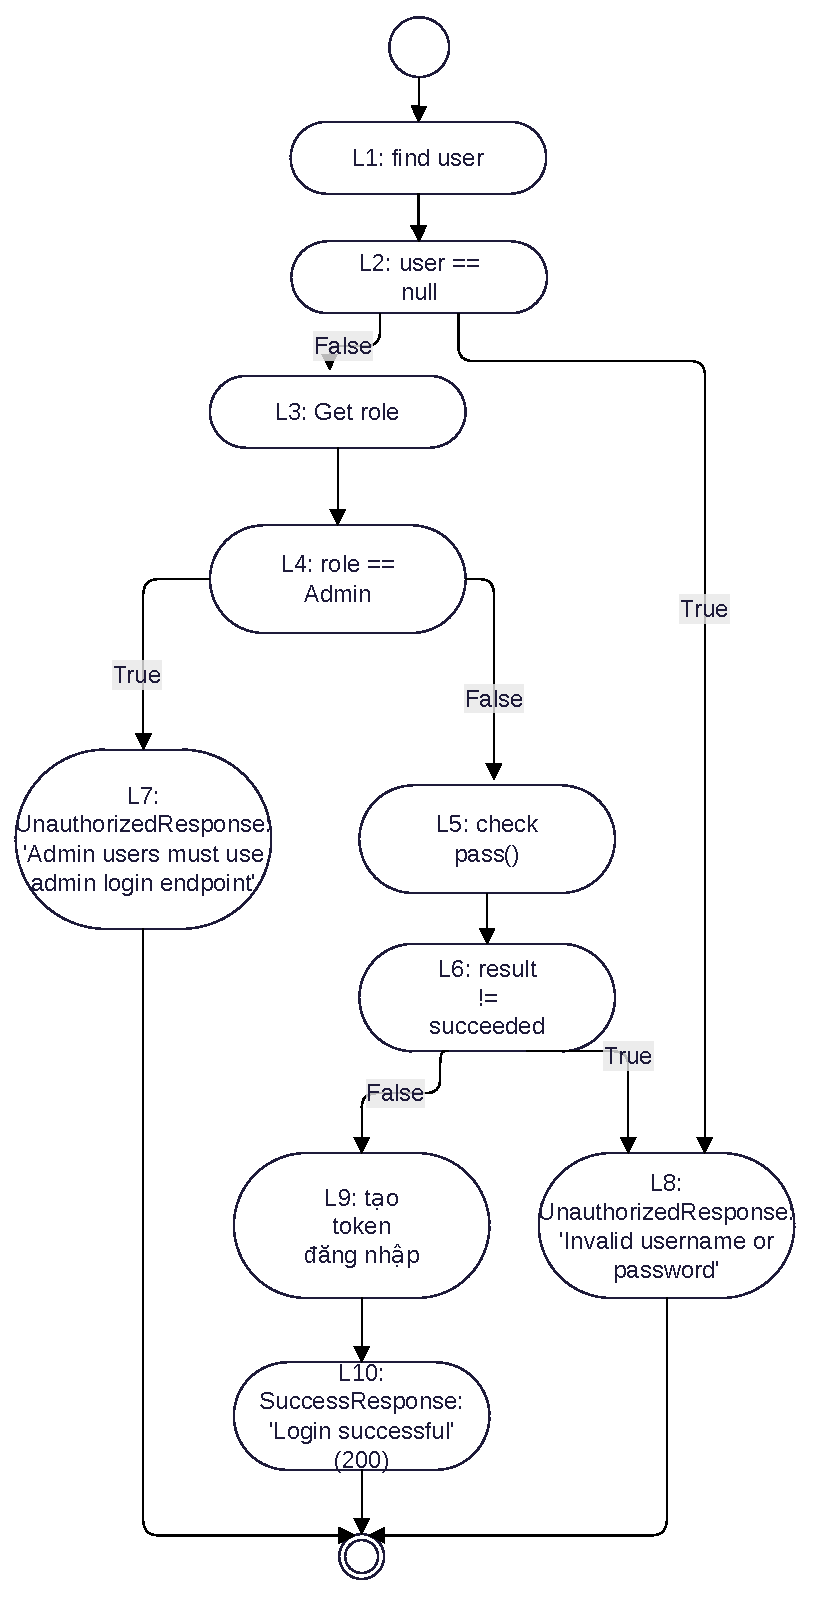
\includegraphics[width=0.62\textwidth]{LoginControlFlow.pdf}
    \caption{Đồ thị dòng điều khiển (CFG) chức năng Đăng nhập người dùng (\texttt{AuthController.Login})}
\end{figure}

\noindent\textbf{e. Độ phức tạp Cyclomatic}
\begin{itemize}[leftmargin=1.2cm, noitemsep]
    \item[\textbf{--}] \textbf{Thông số đồ thị dòng điều khiển (CFG):} Số cạnh $E = 14$, số nút $N = 12$ (gồm \texttt{Start}, \texttt{End} và các nút \texttt{L1}--\texttt{L10}), số thành phần liên thông $P = 1$, số nút quyết định nhị phân $D = 3$ (\texttt{L2, L4, L6}).
    \item[\textbf{--}] \textbf{Độ phức tạp Cyclomatic:}
    \[
        V(G) = E - N + 2P = 14 - 12 + 2 \times 1 = 4 \quad (\text{kiểm tra lại: } V(G) = D + 1 = 3 + 1 = 4)
    \]
    Do đó, tập cơ sở gồm \textbf{4 đường độc lập}.
\end{itemize}

\noindent\textbf{f. Các đường độc lập}

\begin{table}[H]
\centering
\small
\begin{tabularx}{\textwidth}{|C{1.4cm}|L{6.8cm}|X|}
\hline
\rowcolor[RGB]{179, 205, 255}
\textbf{Đường} & \textbf{Chuỗi nút thực thi} & \textbf{Ý nghĩa nghiệp vụ} \tabularnewline
\hline
\textbf{P1} & \texttt{Start} $\rightarrow$ L1 $\rightarrow$ L2 $\rightarrow$ L8 $\rightarrow$ \texttt{End} & Không tìm thấy tài khoản trong CSDL. \\ \hline
\textbf{P2} & \texttt{Start} $\rightarrow$ L1 $\rightarrow$ L2 $\rightarrow$ L3 $\rightarrow$ L4 $\rightarrow$ L7 $\rightarrow$ \texttt{End} & Tài khoản có vai trò Admin bị chặn đăng nhập cổng User. \\ \hline
\textbf{P3} & \texttt{Start} $\rightarrow$ L1 $\rightarrow$ L2 $\rightarrow$ L3 $\rightarrow$ L4 $\rightarrow$ L5 $\rightarrow$ L6 $\rightarrow$ L8 $\rightarrow$ \texttt{End} & Kiểm tra mật khẩu thất bại (sai mật khẩu). \\ \hline
\textbf{P4} & \texttt{Start} $\rightarrow$ L1 $\rightarrow$ L2 $\rightarrow$ L3 $\rightarrow$ L4 $\rightarrow$ L5 $\rightarrow$ L6 $\rightarrow$ L9 $\rightarrow$ L10 $\rightarrow$ \texttt{End} & Đăng nhập thành công, cấp JWT Token và trả HTTP 200. \\ \hline
\end{tabularx}
\caption{Tập 4 đường đi độc lập cơ bản của \texttt{AuthController.Login} (B1)}
\end{table}

\noindent\textbf{Bảng Test Cases chi tiết chức năng B1 (\texttt{AuthController.Login}):}
\begingroup
\scriptsize
\setlength{\tabcolsep}{3pt}
\begin{longtable}{|C{0.8cm}|C{0.75cm}|C{0.95cm}|L{2.0cm}|L{3.0cm}|L{2.25cm}|L{2.6cm}|L{2.5cm}|C{0.85cm}|}
\hline
\rowcolor[RGB]{179, 205, 255}
\textbf{TC\#} & \textbf{BR\#} & \textbf{TR\#} & \textbf{TestCase} & \textbf{TestSteps} & \textbf{Test Data} & \textbf{Expected} & \textbf{Result} & \textbf{P/F} \tabularnewline
\hline
\endfirsthead
\hline
\rowcolor[RGB]{179, 205, 255}
\textbf{TC\#} & \textbf{BR\#} & \textbf{TR\#} & \textbf{TestCase} & \textbf{TestSteps} & \textbf{Test Data} & \textbf{Expected} & \textbf{Result} & \textbf{P/F} \tabularnewline
\hline
\endhead
\hline
\endfoot
\textbf{4} & B1 & T03, T07 & Đăng nhập với tên đăng nhập không tồn tại (P1 -- TC 4) & 1. Vào trang đăng nhập\newline 2. Nhập tên không tồn tại, mật khẩu bất kỳ\newline 3. Nhấn Đăng nhập & Tên: khongtontai999\newline MK: User@123456 & Đăng nhập thất bại, hiển thị ``Invalid username or password''. & Hiển thị ``Invalid username or password''. & \textcolor{blue}{\textbf{Pass}} \\ \hline
\textbf{5} & B1 & T04, T07 & Đăng nhập với mật khẩu sai (P3 -- TC 5) & 1. Vào trang đăng nhập\newline 2. Nhập tên hợp lệ, mật khẩu sai\newline 3. Nhấn Đăng nhập & Tên: User1\newline MK: SaiMatKhau!1 & Đăng nhập thất bại, hiển thị ``Invalid username or password''. & Hiển thị ``Invalid username or password''. & \textcolor{blue}{\textbf{Pass}} \\ \hline
\textbf{6} & B1 & T06, T09 & Đăng nhập thành công với tài khoản User (P4 -- TC 6) & 1. Vào trang đăng nhập\newline 2. Nhập đúng tên và mật khẩu\newline 3. Nhấn Đăng nhập & Tên: User1\newline MK: User@123456 & Đăng nhập thành công, cấp JWT Token, chuyển hướng /home. & Chuyển hướng đến trang Home (/home). & \textcolor{blue}{\textbf{Pass}} \\ \hline
\textbf{9} & B1 & T05 & Đăng nhập bằng tài khoản Admin qua cổng User (P2 -- TC 9) & 1. Vào trang đăng nhập (/login)\newline 2. Nhập TK có vai trò Admin\newline 3. Nhấn Đăng nhập & Tên: admin\newline MK: Admin@123456 & HTTP 401 với thông báo ``Admin users must use admin login endpoint''. & Chặn đăng nhập và hiển thị đúng thông báo. & \textcolor{blue}{\textbf{Pass}} \\ \hline
\caption{Bảng Test Cases hộp trắng chức năng B1 -- AuthController.Login (Control Flow)}
\end{longtable}
\endgroup


\subsubsection{Chức năng B2 -- Đăng ký tài khoản (\texttt{AuthController.Register})}

\noindent\textbf{a. Mô tả chức năng}
\begin{itemize}[leftmargin=1.2cm, noitemsep]
    \item[\textbf{--}] \textbf{Mã BRD:} B2
    \item[\textbf{--}] \textbf{Tên chức năng:} Đăng ký tài khoản (User Registration) -- Xác thực và kiểm tra tính hợp lệ dữ liệu người dùng.
    \item[\textbf{--}] \textbf{Tóm tắt Requirement từ tài liệu hệ thống:}
    \begin{itemize}[leftmargin=0.8cm, label=$\bullet$, noitemsep]
        \item \textbf{Ràng buộc Tên đăng nhập (Username):} Không được để trống; độ dài từ 3 đến 20 ký tự; chỉ chứa chữ cái (\texttt{a-z, A-Z}), chữ số (\texttt{0-9}) và dấu gạch dưới (\texttt{\_}) theo regex \texttt{\^{}[a-zA-Z0-9\_]\{3,20\}\$}; chưa tồn tại trong hệ thống.
        \item \textbf{Ràng buộc Email và Họ tên (Email \& FullName):} Email không được để trống, đúng định dạng qua \texttt{System.Net.Mail.MailAddress} và chưa tồn tại; Họ tên (\texttt{FullName}) không được để trống, độ dài từ 2 đến 100 ký tự sau khi loại bỏ khoảng trắng đầu/cuối.
        \item \textbf{Ràng buộc Mật khẩu và Xác nhận mật khẩu (Password \& Confirmation):} Không được để trống, ít nhất 8 ký tự, chứa tối thiểu 1 chữ hoa (\texttt{A-Z}), 1 chữ thường (\texttt{a-z}), 1 chữ số (\texttt{0-9}) và 1 ký tự đặc biệt (\texttt{!@\#\$\%\^{}*\&(),.?":\{\}|}). Điểm độ mạnh (0--100): $<30$ báo ``Password is too weak''; 30--59 báo ``Password needs improvement''; $\ge 60$ nhưng chưa đủ tiêu chí báo ``Password does not meet requirements''. Mật khẩu xác nhận phải khớp hoàn toàn (``Passwords do not match'').
        \item \textbf{Quy tắc xử lý đăng ký và phân quyền:} Hợp lệ thì tạo tài khoản, gán vai trò ``User'', trả về HTTP 201 Created kèm JWT Token (60 phút). Nếu gán vai trò thất bại, rollback xóa tài khoản và trả HTTP 400 Bad Request.
    \end{itemize}
\end{itemize}

\noindent\textbf{b. Mã nguồn chức năng đăng ký}
\begin{lstlisting}[language={[Sharp]C}]
public async Task<IActionResult> Register([FromBody] RegisterDto registerDto)
{
1:  if (!ValidationHelper.IsValidEmail(registerDto.Email))
2:      return this.BadRequestResponse(new List<ApiError> { ErrorHelper.CreateValidationError("email", "Invalid email format") });
3:  if (!ValidationHelper.IsValidUsername(registerDto.UserName))
4:      return this.BadRequestResponse(new List<ApiError> { ErrorHelper.CreateValidationError("username", "Username must be 3-20 characters, alphanumeric and underscore only") });
5:  if (!ValidationHelper.IsValidFullName(registerDto.FullName))
6:      return this.BadRequestResponse(new List<ApiError> { ErrorHelper.CreateValidationError("fullName", "Full name must be 2-100 characters") });
7:  if (!ValidationHelper.IsStrongPassword(registerDto.Password))
    {
8:      var passwordStrength = ValidationHelper.GetPasswordStrength(registerDto.Password);
9:      var message = passwordStrength < 30 ? "Password is too weak (must contain uppercase, lowercase, number, special char)" :
                      passwordStrength < 60 ? "Password needs improvement (at least 8 chars)" :
                      "Password does not meet requirements";
10:     return this.BadRequestResponse(new List<ApiError> { ErrorHelper.CreateValidationError("password", message) });
    }
11: var existingUser = await _userManager.FindByNameAsync(registerDto.UserName);
12: if (existingUser != null)
13:     return this.BadRequestResponse(new List<ApiError> { ErrorHelper.CreateValidationError("username", "Username already exists") });
14: var existingEmail = await _userManager.FindByEmailAsync(registerDto.Email);
15: if (existingEmail != null)
16:     return this.BadRequestResponse(new List<ApiError> { ErrorHelper.CreateValidationError("email", "Email already registered") });
17: var user = new User { UserName = registerDto.UserName, Email = registerDto.Email, FullName = registerDto.FullName };
18: var result = await _userManager.CreateAsync(user, registerDto.Password);
19: if (!result.Succeeded)
    {
20:     var errors = result.Errors.Select(e => new ApiError(e.Description, code: AppErrorCodes.VALIDATION_ERROR)).ToList();
21:     return this.BadRequestResponse(errors);
    }
22: var roleResult = await _userManager.AddToRoleAsync(user, RoleConstants.User);
23: if (!roleResult.Succeeded)
    {
24:     await _userManager.DeleteAsync(user); // Rollback neu gan role that bai
25:     var errors = roleResult.Errors.Select(e => new ApiError(e.Description, code: AppErrorCodes.INVALID_STATE)).ToList();
26:     return this.BadRequestResponse(errors);
    }
27: var token = await GenerateJwtToken(user);
28: var authData = new
    {
        Token = token,
        User = new UserResponseDto
        {
            Id = user.Id,
            UserName = user.UserName ?? string.Empty,
            Email = user.Email ?? string.Empty,
            FullName = user.FullName ?? string.Empty,
            ProfilePictureUrl = user.ProfilePictureUrl
        }
    };
29: return this.CreatedResponse(authData, "Registration successful");
}
\end{lstlisting}

\noindent\textbf{c. Các điều kiện quyết định và nút xử lý}
\begin{table}[H]
\centering
\small
\begin{tabularx}{\textwidth}{|L{3.2cm}|X|}
\hline
\rowcolor[RGB]{179, 205, 255}
\textbf{Nhãn} & \textbf{Nút xử lý trên sơ đồ} \tabularnewline
\hline
\textbf{A1, A2, A3} & Lỗi email; lỗi tên đăng nhập; lỗi họ tên \\ \hline
\textbf{A4} & Tính điểm mật khẩu \\ \hline
\textbf{A5, A6, A7} & Ba thông báo lỗi mật khẩu, theo thứ tự điểm $<30$, $<60$, $\ge 60$ \\ \hline
\textbf{A8, A9} & Tìm theo tên đăng nhập; lỗi tên đã tồn tại \\ \hline
\textbf{A10, A11} & Tìm theo email; lỗi email đã tồn tại \\ \hline
\textbf{A12, A13} & Tạo tài khoản; lập lỗi \texttt{VALIDATION\_ERROR} \\ \hline
\textbf{A14, A15, A16} & Gán vai trò; xóa tài khoản vừa tạo; lập lỗi \texttt{INVALID\_STATE} \\ \hline
\textbf{A17, A18, A19} & Tạo JWT; trả HTTP 201; trả HTTP 400 \\ \hline
\end{tabularx}
\caption{Bảng mô tả các nút xử lý (\texttt{A1}--\texttt{A19}) của hàm \texttt{Register} (B2)}
\end{table}

\begin{table}[H]
\centering
\small
\begin{tabularx}{\textwidth}{|C{1.8cm}|X|}
\hline
\rowcolor[RGB]{179, 205, 255}
\textbf{Nút} & \textbf{Điều kiện trong mã nguồn} \tabularnewline
\hline
\textbf{R1} & \texttt{!ValidationHelper.IsValidEmail(registerDto.Email)} \\ \hline
\textbf{R2} & \texttt{!ValidationHelper.IsValidUsername(registerDto.UserName)} \\ \hline
\textbf{R3} & \texttt{!ValidationHelper.IsValidFullName(registerDto.FullName)} \\ \hline
\textbf{R4} & \texttt{!ValidationHelper.IsStrongPassword(registerDto.Password)} \\ \hline
\textbf{R5} & \texttt{passwordStrength < 30} \\ \hline
\textbf{R6} & \texttt{passwordStrength < 60} \\ \hline
\textbf{R7} & \texttt{existingUser != null} \\ \hline
\textbf{R8} & \texttt{existingEmail != null} \\ \hline
\textbf{R9} & \texttt{!result.Succeeded} \\ \hline
\textbf{R10} & \texttt{!roleResult.Succeeded} \\ \hline
\end{tabularx}
\caption{Bảng mô tả các nút điều kiện quyết định (\texttt{R1}--\texttt{R10}) của hàm \texttt{Register} (B2)}
\end{table}

\noindent\textbf{d. Đồ thị dòng điều khiển (CFG)}
\begin{figure}[H]
    \centering
    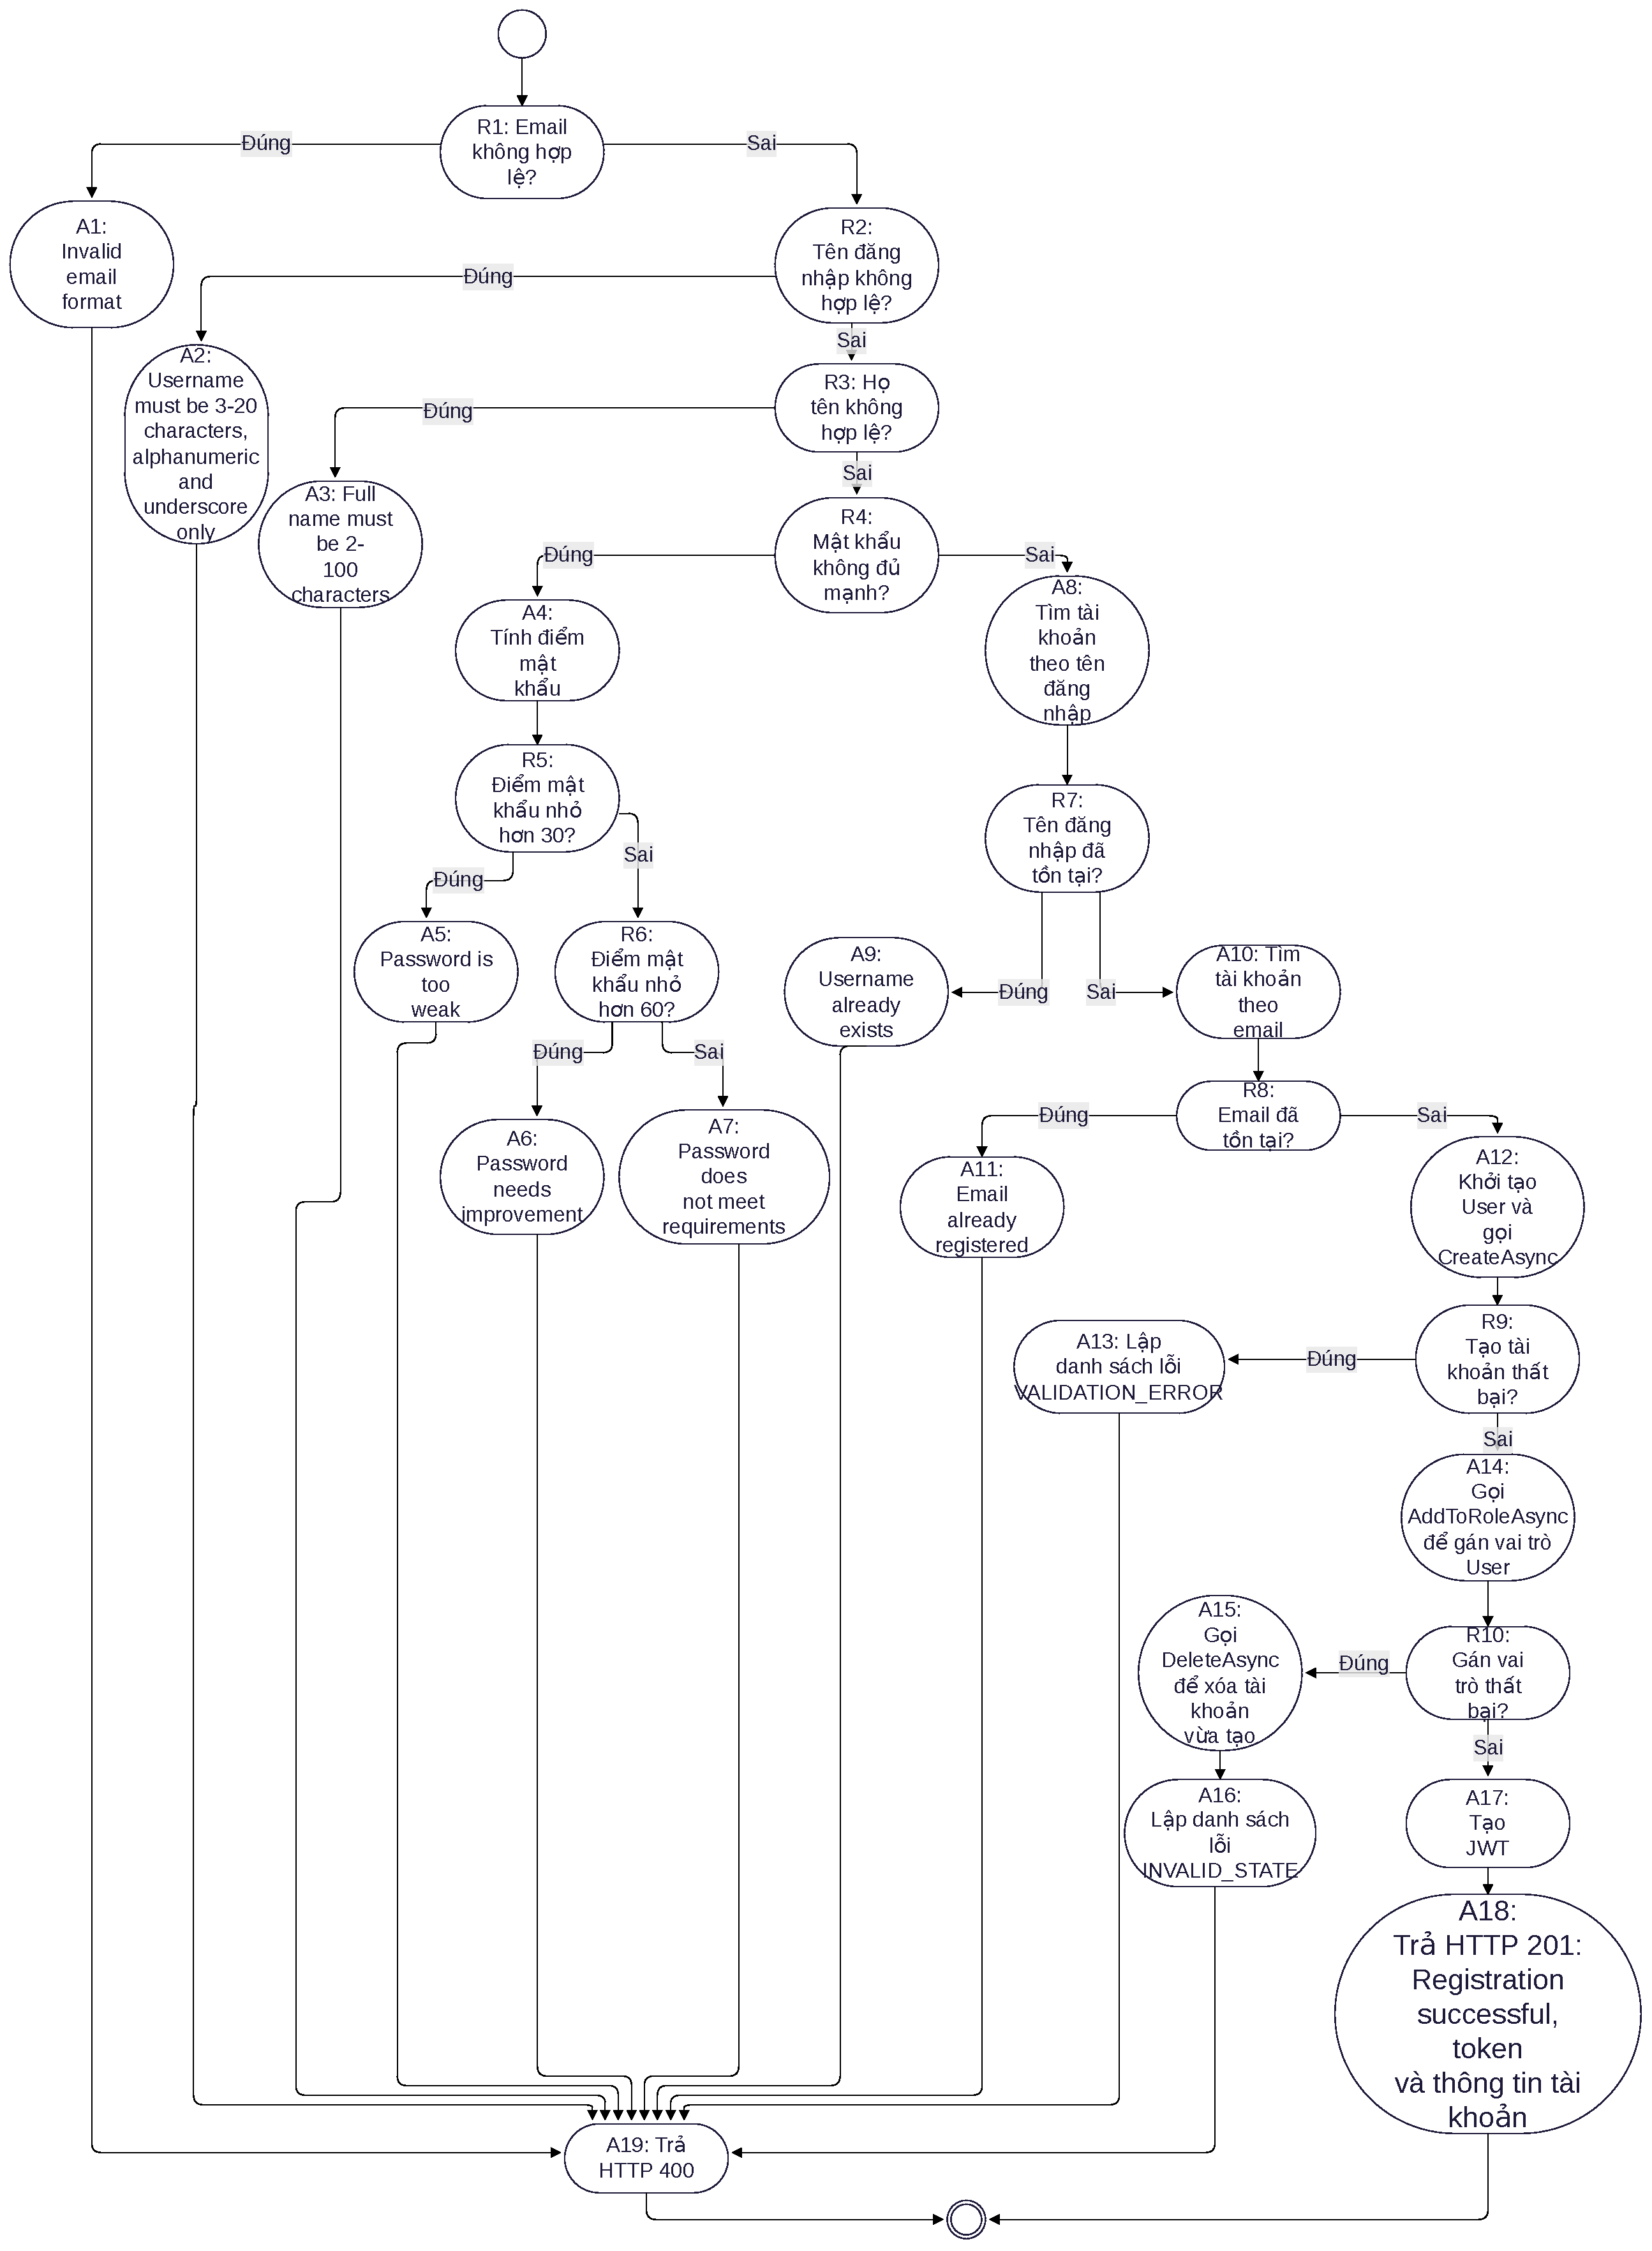
\includegraphics[width=1\textwidth]{RegisterControlFlow.pdf}
    \caption{Đồ thị dòng điều khiển (CFG) chức năng Đăng ký tài khoản (\texttt{AuthController.Register})}
\end{figure}

\noindent\textbf{e. Độ phức tạp Cyclomatic}
\begin{itemize}[leftmargin=1.2cm, noitemsep]
    \item[\textbf{--}] \textbf{Thông số đồ thị dòng điều khiển (CFG):} Số cạnh $E = 40$, số nút $N = 31$ (gồm \texttt{Start}, \texttt{End}), số thành phần liên thông $P = 1$, số nút quyết định nhị phân $D = 10$ (\texttt{R1}--\texttt{R10}).
    \item[\textbf{--}] \textbf{Độ phức tạp Cyclomatic:}
    \[
        V(G) = E - N + 2P = 40 - 31 + 2 \times 1 = 11 \quad (\text{kiểm tra lại: } V(G) = D + 1 = 10 + 1 = 11)
    \]
    Do đó, tập cơ sở gồm \textbf{11 đường độc lập}.
\end{itemize}

\noindent\textbf{f. Các đường độc lập}

\begin{longtable}{|C{1.3cm}|L{8.3cm}|L{6.2cm}|}
\hline
\rowcolor[RGB]{179, 205, 255}
\textbf{Đường} & \textbf{Chuỗi nút thực thi} & \textbf{Ý nghĩa nghiệp vụ} \tabularnewline
\hline
\endfirsthead
\hline
\rowcolor[RGB]{179, 205, 255}
\textbf{Đường} & \textbf{Chuỗi nút thực thi} & \textbf{Ý nghĩa nghiệp vụ} \tabularnewline
\hline
\endhead
\hline
\endfoot
\textbf{Q1} & \texttt{Start} $\rightarrow$ R1 $\rightarrow$ A1 $\rightarrow$ A19 $\rightarrow$ \texttt{End} & Email không hợp lệ. \\ \hline
\textbf{Q2} & \texttt{Start} $\rightarrow$ R1 $\rightarrow$ R2 $\rightarrow$ A2 $\rightarrow$ A19 $\rightarrow$ \texttt{End} & Tên đăng nhập không hợp lệ. \\ \hline
\textbf{Q3} & \texttt{Start} $\rightarrow$ R1 $\rightarrow$ R2 $\rightarrow$ R3 $\rightarrow$ A3 $\rightarrow$ A19 $\rightarrow$ \texttt{End} & Họ tên không hợp lệ. \\ \hline
\textbf{Q4} & \texttt{Start} $\rightarrow$ R1 $\rightarrow$ R2 $\rightarrow$ R3 $\rightarrow$ R4 $\rightarrow$ A4 $\rightarrow$ R5 $\rightarrow$ A5 $\rightarrow$ A19 $\rightarrow$ \texttt{End} & Mật khẩu không đạt, điểm $< 30$. \\ \hline
\textbf{Q5} & \texttt{Start} $\rightarrow$ R1 $\rightarrow$ R2 $\rightarrow$ R3 $\rightarrow$ R4 $\rightarrow$ A4 $\rightarrow$ R5 $\rightarrow$ R6 $\rightarrow$ A6 $\rightarrow$ A19 $\rightarrow$ \texttt{End} & Mật khẩu không đạt, điểm $30\text{--}59$. \\ \hline
\textbf{Q6} & \texttt{Start} $\rightarrow$ R1 $\rightarrow$ R2 $\rightarrow$ R3 $\rightarrow$ R4 $\rightarrow$ A4 $\rightarrow$ R5 $\rightarrow$ R6 $\rightarrow$ A7 $\rightarrow$ A19 $\rightarrow$ \texttt{End} & Mật khẩu không đạt, điểm $\ge 60$. \\ \hline
\textbf{Q7} & \texttt{Start} $\rightarrow$ R1 $\rightarrow$ R2 $\rightarrow$ R3 $\rightarrow$ R4 $\rightarrow$ A8 $\rightarrow$ R7 $\rightarrow$ A9 $\rightarrow$ A19 $\rightarrow$ \texttt{End} & Tên đăng nhập đã tồn tại. \\ \hline
\textbf{Q8} & \texttt{Start} $\rightarrow$ R1 $\rightarrow$ R2 $\rightarrow$ R3 $\rightarrow$ R4 $\rightarrow$ A8 $\rightarrow$ R7 $\rightarrow$ A10 $\rightarrow$ R8 $\rightarrow$ A11 $\rightarrow$ A19 $\rightarrow$ \texttt{End} & Email đã được đăng ký. \\ \hline
\textbf{Q9} & \texttt{Start} $\rightarrow$ R1 $\rightarrow$ R2 $\rightarrow$ R3 $\rightarrow$ R4 $\rightarrow$ A8 $\rightarrow$ R7 $\rightarrow$ A10 $\rightarrow$ R8 $\rightarrow$ A12 $\rightarrow$ R9 $\rightarrow$ A13 $\rightarrow$ A19 $\rightarrow$ \texttt{End} & Tạo tài khoản thất bại. \\ \hline
\textbf{Q10} & \texttt{Start} $\rightarrow$ R1 $\rightarrow$ R2 $\rightarrow$ R3 $\rightarrow$ R4 $\rightarrow$ A8 $\rightarrow$ R7 $\rightarrow$ A10 $\rightarrow$ R8 $\rightarrow$ A12 $\rightarrow$ R9 $\rightarrow$ A14 $\rightarrow$ R10 $\rightarrow$ A15 $\rightarrow$ A16 $\rightarrow$ A19 $\rightarrow$ \texttt{End} & Gán vai trò thất bại (rollback). \\ \hline
\textbf{Q11} & \texttt{Start} $\rightarrow$ R1 $\rightarrow$ R2 $\rightarrow$ R3 $\rightarrow$ R4 $\rightarrow$ A8 $\rightarrow$ R7 $\rightarrow$ A10 $\rightarrow$ R8 $\rightarrow$ A12 $\rightarrow$ R9 $\rightarrow$ A14 $\rightarrow$ R10 $\rightarrow$ A17 $\rightarrow$ A18 $\rightarrow$ \texttt{End} & Đăng ký tài khoản thành công. \\ \hline
\end{longtable}

\noindent\textbf{Bảng Test Cases chi tiết chức năng B2 (\texttt{AuthController.Register}):}
\begingroup
\scriptsize
\setlength{\tabcolsep}{3pt}
\begin{longtable}{|C{0.8cm}|C{0.75cm}|C{0.95cm}|L{2.0cm}|L{3.0cm}|L{2.25cm}|L{2.6cm}|L{2.5cm}|C{0.85cm}|}
\hline
\rowcolor[RGB]{179, 205, 255}
\textbf{TC\#} & \textbf{BR\#} & \textbf{TR\#} & \textbf{TestCase} & \textbf{TestSteps} & \textbf{Test Data} & \textbf{Expected} & \textbf{Result} & \textbf{P/F} \tabularnewline
\hline
\endfirsthead
\hline
\rowcolor[RGB]{179, 205, 255}
\textbf{TC\#} & \textbf{BR\#} & \textbf{TR\#} & \textbf{TestCase} & \textbf{TestSteps} & \textbf{Test Data} & \textbf{Expected} & \textbf{Result} & \textbf{P/F} \tabularnewline
\hline
\endhead
\hline
\endfoot
\textbf{12} & B2 & T12 & Đăng ký với Tên đăng nhập 2 ký tự (Q2 -- TC 12) & 1. Vào trang đăng ký\newline 2. Nhập tên đăng nhập 2 ký tự, nhấn Đăng ký & Tên: ab\newline MK: Aa123456! & Đăng ký thất bại, báo ``Username must be 3-20 characters...''. & Hiển thị thông báo lỗi độ dài Username. & \textcolor{blue}{\textbf{Pass}} \\ \hline
\textbf{17} & B2 & T15 & Đăng ký với Tên đăng nhập đã tồn tại (Q7 -- TC 17) & 1. Vào trang đăng ký\newline 2. Nhập Username đã tồn tại, nhấn Đăng ký & Tên: User1\newline MK: Aa123456! & Đăng ký thất bại, báo ``Username already exists''. & Hiển thị ``Username already exists''. & \textcolor{blue}{\textbf{Pass}} \\ \hline
\textbf{19} & B2 & T17 & Đăng ký với Email sai định dạng (Q1 -- TC 19) & 1. Vào trang đăng ký\newline 2. Nhập email sai định dạng, nhấn Đăng ký & Email: new\_user@example & Đăng ký thất bại, thông báo ``Invalid email format''. & Hiển thị ``Invalid email format''. & \textcolor{blue}{\textbf{Pass}} \\ \hline
\textbf{20} & B2 & T18 & Đăng ký với Email đã tồn tại (Q8 -- TC 20) & 1. Vào trang đăng ký\newline 2. Nhập Email đã có trong hệ thống, nhấn Đăng ký & Email: user1@test.com & Đăng ký thất bại, báo ``Email already registered''. & Hiển thị ``Email already registered''. & \textcolor{blue}{\textbf{Pass}} \\ \hline
\textbf{22} & B2 & T20 & Đăng ký với Họ tên 1 ký tự (Q3 -- TC 22) & 1. Vào trang đăng ký\newline 2. Nhập họ tên 1 ký tự, nhấn Đăng ký & HT: A\newline MK: Aa123456! & Đăng ký thất bại, báo ``Full name must be 2-100 characters''. & Hiển thị thông báo lỗi độ dài Họ tên. & \textcolor{blue}{\textbf{Pass}} \\ \hline
\textbf{34} & B2 & T30, T32 & Đăng ký thành công với thông tin hợp lệ (Q11 -- TC 34) & 1. Vào trang đăng ký\newline 2. Điền đầy đủ thông tin hợp lệ, nhấn Đăng ký & Tên: new\_user\newline MK: Aa123456! & Đăng ký thành công, tạo tài khoản, gán role ``User'', về /login. & Đăng ký thành công, chuyển về /login. & \textcolor{blue}{\textbf{Pass}} \\ \hline
\textbf{37} & B2 & T28 & Mật khẩu không đạt, điểm độ mạnh $< 30$ (Q4 -- TC 37) & 1. Chuẩn bị Email, Username, FullName hợp lệ\newline 2. Gửi API Register với MK yếu ($<30$ điểm) & MK: \texttt{123} (điểm $< 30$) & HTTP 400 Bad Request ``Password is too weak (must contain uppercase, lowercase, number, special char)''. & API trả về HTTP 400 Bad Request kèm thông báo ``Password is too weak (must contain uppercase, lowercase, number, special char)''. & \textcolor{blue}{\textbf{Pass}} \\ \hline
\textbf{38} & B2 & T23, T28 & Mật khẩu không đạt, điểm độ mạnh $30\text{--}59$ (Q5 -- TC 38) & 1. Gửi API Register với MK trung bình (30--59 điểm, tương tự TC 27 ở ngưỡng 30--59) & MK: \texttt{abc1234} (điểm $30\text{--}59$) & HTTP 400 Bad Request ``Password needs improvement (at least 8 chars)''. & API trả về HTTP 400 Bad Request kèm thông báo ``Password needs improvement (at least 8 chars)''. & \textcolor{blue}{\textbf{Pass}} \\ \hline
\textbf{39} & B2 & T24--T28 & Mật khẩu không đạt, điểm $\ge 60$ nhưng thiếu tiêu chí (Q6 -- TC 39) & 1. Gửi API Register với MK $\ge 8$ ký tự ($\ge 60$ điểm) nhưng thiếu ký tự đặc biệt & MK: \texttt{Aa12345678} (điểm $\ge 60$) & HTTP 400 Bad Request ``Password does not meet requirements''. & API trả về HTTP 400 Bad Request kèm thông báo ``Password does not meet requirements''. & \textcolor{blue}{\textbf{Pass}} \\ \hline
\textbf{40} & B2 & T33 & Tạo tài khoản thất bại tại Identity \texttt{CreateAsync} (Q9 -- TC 40) & 1. Giả lập \texttt{CreateAsync} trả \texttt{Succeeded = false}\newline 2. Gọi \texttt{AuthController.Register} & Dữ liệu hợp lệ; Mock \texttt{CreateAsync} lỗi & HTTP 400 Bad Request kèm danh sách lỗi mã \texttt{VALIDATION\_ERROR}. & API trả về HTTP 400 Bad Request kèm danh sách lỗi mã \texttt{VALIDATION\_ERROR}. & \textcolor{blue}{\textbf{Pass}} \\ \hline
\textbf{41} & B2 & T31 & Gán vai trò thất bại và rollback xóa tài khoản (Q10 -- TC 41) & 1. Mock \texttt{CreateAsync} thành công\newline 2. Mock \texttt{AddToRoleAsync} thất bại, kiểm tra gọi \texttt{DeleteAsync} & Dữ liệu hợp lệ; Mock \texttt{AddToRoleAsync} lỗi & Gọi \texttt{DeleteAsync(user)} để rollback và trả HTTP 400 mã \texttt{INVALID\_STATE}. & Hệ thống gọi \texttt{DeleteAsync(user)} để rollback và trả về HTTP 400 mã \texttt{INVALID\_STATE}. & \textcolor{blue}{\textbf{Pass}} \\ \hline
\caption{Bảng Test Cases hộp trắng chức năng B2 -- AuthController.Register (đủ 11 đường độc lập Q1--Q11)}
\end{longtable}
\endgroup


% ----------------------------------------------------------
% 4.2 Data Flow Testing
% ----------------------------------------------------------
\subsection{Kiểm thử dòng dữ liệu (Data Flow Testing)}

\subsubsection{Chức năng B7 -- Kết bạn \& Mạng lưới kết nối (\texttt{SendFriendRequestAsync})}

\noindent\textbf{a. Mô tả nghiệp vụ \& Yêu cầu kỹ thuật (TRD)}
\begin{itemize}[leftmargin=1.2cm, noitemsep]
    \item[\textbf{--}] \textbf{Mã BRD:} B7.
    \item[\textbf{--}] \textbf{Tên chức năng:} Gửi lời mời kết bạn (\texttt{SendFriendRequestAsync}).
    \item[\textbf{--}] \textbf{Mục đích:} Cho phép người dùng gửi lời mời kết bạn tới một người dùng khác hợp lệ trong hệ thống, lưu trạng thái chờ duyệt (\texttt{Pending}) và phát thông báo thời gian thực.
    \item[\textbf{--}] \textbf{Tiền điều kiện:} Người gửi (\texttt{senderId}) và người nhận (\texttt{receiverId}) là các định danh tài khoản hợp lệ được truyền vào dịch vụ xử lý kết bạn.
    \item[\textbf{--}] \textbf{Yêu cầu nghiệp vụ liên quan:}
    \begin{itemize}[leftmargin=0.8cm, label=$\bullet$, noitemsep]
        \item Không cho phép người dùng tự gửi lời mời kết bạn cho chính mình (\texttt{senderId == receiverId}).
        \item Không cho phép gửi lời mời kết bạn tới tài khoản có vai trò Quản trị viên (\texttt{Admin}).
        \item Không cho phép gửi lời mời trùng lặp nếu giữa hai người dùng đã có quan hệ chờ duyệt (\texttt{Pending}) hoặc đã là bạn bè (\texttt{Accepted}).
        \item Khi hợp lệ, lưu quan hệ kết bạn mới với trạng thái \texttt{Pending}, gửi thông báo qua \texttt{NotifyFriendRequestAsync} và trả về đối tượng \texttt{Friendship}.
    \end{itemize}
\end{itemize}

\begin{table}[H]
\centering
\small
\begin{tabularx}{\textwidth}{|C{1.8cm}|X|}
\hline
\rowcolor[RGB]{179, 205, 255}
\textbf{Mã TRD} & \textbf{Mô tả yêu cầu} \tabularnewline
\hline
\textbf{T97} & Không thể tự gửi lời mời kết bạn cho chính mình; hệ thống chặn thao tác nếu \texttt{senderId == receiverId}. \\ \hline
\textbf{T98} & Không cho phép gửi lời mời kết bạn trùng lặp khi giữa hai người đã tồn tại lời mời \texttt{Pending} hoặc đã là bạn bè (\texttt{Accepted}). \\ \hline
\textbf{T99} & Lời mời kết bạn mới được lưu ở trạng thái Chờ duyệt (\texttt{Pending}) và phát thông báo thời gian thực tới người nhận. \\ \hline
\textbf{T106.1} & Không cho phép người dùng gửi lời mời kết bạn tới tài khoản có vai trò Quản trị viên (\texttt{Admin}); hệ thống chặn thao tác và ném ngoại lệ nghiệp vụ. \\ \hline
\end{tabularx}
\caption{Bảng mô tả các yêu cầu kỹ thuật (TRD) liên quan đến chức năng gửi lời mời kết bạn (B7)}
\end{table}

\noindent\textbf{b. Mã nguồn đối tượng kiểm thử (\texttt{SendFriendRequestAsync})}
\begin{lstlisting}[language={[Sharp]C}]
public async Task<Friendship> SendFriendRequestAsync(string senderId, string receiverId)
{
1:  if (senderId == receiverId)
2:      throw new InvalidOperationException("Khong the gui loi moi ket ban cho chinh minh");

3:  var adminRoleId = await _roleRepository.GetRoleIdByNameAsync("Admin");
4:  if (adminRoleId != null)
    {
5:      var isReceiverAdmin = await _userRoleRepository.IsUserInRoleAsync(receiverId, adminRoleId);
6:      if (isReceiverAdmin)
7:          throw new InvalidOperationException("Khong the gui loi moi ket ban cho tai khoan nay");
    }

8:  var existingRequest = await _friendshipRepository.GetExistingAsync(senderId, receiverId);
9:  if (existingRequest != null)
10:     throw new InvalidOperationException("Loi moi ket ban da ton tai hoac da la ban be");

11: var friendship = new Friendship { SenderId = senderId, ReceiverId = receiverId, Status = "Pending" };
12: await _friendshipRepository.AddAsync(friendship);
13: await _notificationService.NotifyFriendRequestAsync(senderId, receiverId);
14: return friendship;
}
\end{lstlisting}

\noindent\textbf{c. Xác định các biến cần kiểm thử và điểm định nghĩa (\texttt{d}) -- sử dụng (\texttt{u})}
Các thao tác đối với biến được ký hiệu: \texttt{d} (\textit{define} -- định nghĩa/gán giá trị), \texttt{u} (\textit{use} -- sử dụng giá trị trong điều kiện, biểu thức, lời gọi hàm hoặc câu lệnh trả về), \texttt{k} (\textit{kill} -- kết thúc phạm vi tồn tại của biến).

\begin{table}[H]
\centering
\scriptsize
\begin{tabularx}{\textwidth}{|L{2.3cm}|L{3.1cm}|L{3.2cm}|X|}
\hline
\rowcolor[RGB]{179, 205, 255}
\textbf{Biến} & \textbf{Ý nghĩa} & \textbf{Điểm định nghĩa (\texttt{d})} & \textbf{Điểm sử dụng (\texttt{u})} \tabularnewline
\hline
\texttt{senderId} & Mã người gửi lời mời & \texttt{Start}: nhận tham số đầu vào & \texttt{F1}: so sánh \texttt{senderId == receiverId}; \texttt{F8}: truyền vào \texttt{GetExistingAsync}; \texttt{F11}: khởi tạo \texttt{Friendship}; \texttt{F13}: truyền vào \texttt{NotifyFriendRequestAsync}. \\ \hline
\texttt{receiverId} & Mã người nhận lời mời & \texttt{Start}: nhận tham số đầu vào & \texttt{F1}: so sánh với \texttt{senderId}; \texttt{F5}: truyền vào \texttt{IsUserInRoleAsync}; \texttt{F8}: truyền vào \texttt{GetExistingAsync}; \texttt{F11}: khởi tạo \texttt{Friendship}; \texttt{F13}: truyền vào \texttt{NotifyFriendRequestAsync}. \\ \hline
\texttt{adminRoleId} & Mã vai trò \texttt{Admin} trong hệ thống & \texttt{F3}: nhận kết quả từ \texttt{GetRoleIdByNameAsync} & \texttt{F4}: kiểm tra \texttt{adminRoleId != null}; \texttt{F5}: truyền vào \texttt{IsUserInRoleAsync}. \\ \hline
\texttt{isReceiverAdmin} & Cờ kiểm tra người nhận có phải \texttt{Admin} & \texttt{F5}: nhận kết quả từ \texttt{IsUserInRoleAsync} & \texttt{F6}: kiểm tra điều kiện \texttt{if (isReceiverAdmin)}. \\ \hline
\texttt{existingRequest} & Quan hệ kết bạn đã tồn tại (nếu có) & \texttt{F8}: nhận kết quả từ \texttt{GetExistingAsync} & \texttt{F9}: kiểm tra điều kiện \texttt{if (existingRequest != null)}. \\ \hline
\texttt{friendship} & Đối tượng quan hệ kết bạn mới tạo & \texttt{F11}: khởi tạo \texttt{new Friendship} & \texttt{F12}: truyền vào \texttt{AddAsync}; \texttt{F14}: trả về kết quả \texttt{return friendship}. \\ \hline
\end{tabularx}
\caption{Bảng xác định các biến và thao tác định nghĩa -- sử dụng theo nút \texttt{F} (\texttt{SendFriendRequestAsync})}
\end{table}

\noindent\textbf{d. Ánh xạ các nút và Đồ thị dòng dữ liệu theo Quy trình kiểm thử dòng dữ liệu}

\begin{table}[H]
\centering
\scriptsize
\begin{tabularx}{\textwidth}{|C{1.3cm}|X|L{5.5cm}|}
\hline
\rowcolor[RGB]{179, 205, 255}
\textbf{Nút} & \textbf{Nội dung xử lý} & \textbf{Thao tác với biến} \tabularnewline
\hline
\textbf{Start} & Nhận tham số đầu vào \texttt{senderId} và \texttt{receiverId} & \texttt{d(senderId), d(receiverId)} \\ \hline
\textbf{F1} & Kiểm tra người gửi có trùng người nhận (\texttt{senderId == receiverId}) & \texttt{u(senderId), u(receiverId)} \\ \hline
\textbf{F2} & Ném ngoại lệ không thể tự kết bạn với chính mình & Không có thao tác đọc hoặc gán các biến đang xét \\ \hline
\textbf{F3} & Lấy mã vai trò \texttt{Admin} qua \texttt{GetRoleIdByNameAsync("Admin")} & \texttt{d(adminRoleId)} \\ \hline
\textbf{F4} & Kiểm tra vai trò \texttt{Admin} có tồn tại (\texttt{adminRoleId != null}) & \texttt{u(adminRoleId)} \\ \hline
\textbf{F5} & Kiểm tra người nhận có vai trò \texttt{Admin} qua \texttt{IsUserInRoleAsync} & \texttt{u(receiverId), u(adminRoleId), d(isReceiverAdmin)} \\ \hline
\textbf{F6} & Kiểm tra kết quả \texttt{if (isReceiverAdmin)} & \texttt{u(isReceiverAdmin)} \\ \hline
\textbf{F7} & Ném ngoại lệ từ chối gửi lời mời tới tài khoản \texttt{Admin} & Không có thao tác đọc hoặc gán các biến đang xét \\ \hline
\textbf{F8} & Truy vấn quan hệ hiện có \texttt{GetExistingAsync(senderId, receiverId)} & \texttt{u(senderId), u(receiverId), d(existingRequest)} \\ \hline
\textbf{F9} & Kiểm tra quan hệ đã tồn tại chưa (\texttt{existingRequest != null}) & \texttt{u(existingRequest)} \\ \hline
\textbf{F10} & Ném ngoại lệ lời mời đã tồn tại hoặc đã là bạn bè & Không có thao tác đọc hoặc gán các biến đang xét \\ \hline
\textbf{F11} & Khởi tạo thực thể \texttt{Friendship} với trạng thái \texttt{Pending} & \texttt{u(senderId), u(receiverId), d(friendship)} \\ \hline
\textbf{F12} & Lưu lời mời kết bạn vào cơ sở dữ liệu qua \texttt{AddAsync} & \texttt{u(friendship)} \\ \hline
\textbf{F13} & Gửi thông báo lời mời kết bạn qua \texttt{NotifyFriendRequestAsync} & \texttt{u(senderId), u(receiverId)} \\ \hline
\textbf{F14} & Trả về đối tượng \texttt{friendship} vừa tạo & \texttt{u(friendship)} \\ \hline
\textbf{End} & Kết thúc thực thi hàm & \texttt{k(all)} đối với các tham số và biến cục bộ còn hiệu lực \\ \hline
\end{tabularx}
\caption{Bảng ánh xạ các nút và thao tác với biến trong đồ thị dòng dữ liệu (\texttt{F1}--\texttt{F14})}
\end{table}

\begin{figure}[H]
\centering
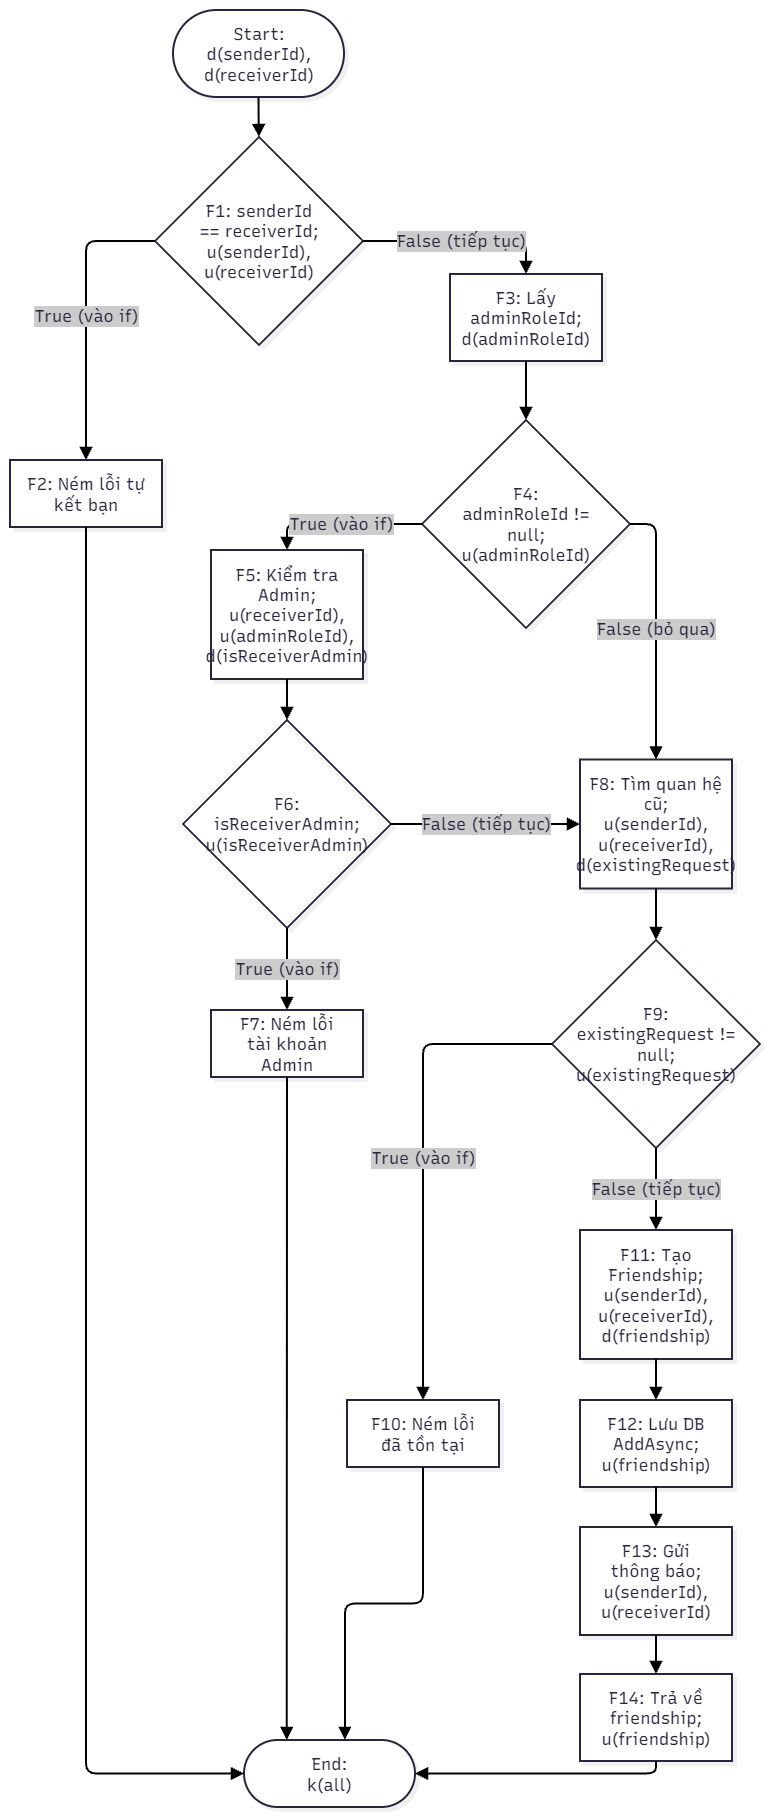
\includegraphics[width=0.92\textwidth,height=0.78\textheight,keepaspectratio]{FriendRequestDataFlow.png}
\caption{Đồ thị dòng dữ liệu (DFG) tổng hợp chức năng gửi lời mời kết bạn (\texttt{SendFriendRequestAsync})}
\end{figure}

\begin{itemize}[leftmargin=1.2cm, noitemsep]
    \item[\textbf{--}] \textbf{Thông số đồ thị dòng dữ liệu:} Số nút $N = 16$ (\texttt{Start}, \texttt{End} và \texttt{F1}--\texttt{F14}), số cạnh $E = 19$, số nút quyết định $D = 4$ (\texttt{F1, F4, F6, F9}).
    \item[\textbf{--}] \textbf{Độ phức tạp Cyclomatic:} $M = V(G) = E - N + 2 = 19 - 16 + 2 = 5$ (kiểm tra đối chiếu: $V(G) = D + 1 = 4 + 1 = 5$).
    \item[\textbf{--}] \textbf{6 biến được theo dõi định nghĩa (\texttt{d}), sử dụng (\texttt{u}) và kết thúc (\texttt{k}):} \texttt{senderId}, \texttt{receiverId}, \texttt{adminRoleId}, \texttt{isReceiverAdmin}, \texttt{existingRequest}, \texttt{friendship}.
\end{itemize}

% Helper macro vẽ sơ đồ DFG thu gọn cho từng biến của SendFriendRequestAsync
\newcommand{\DrawFriendRequestVarDFG}{%
\begin{tikzpicture}[
    baseline=(S.north),
    >=Stealth,
    vnode/.style={circle, draw=black, minimum size=0.72cm, inner sep=0.5pt, font=\scriptsize\ttfamily\bfseries, align=center},
    startnode/.style={circle, draw=black, fill=green!70!teal, minimum size=0.28cm, inner sep=0pt},
    endnode/.style={circle, draw=black, double, fill=green!70!teal, minimum size=0.28cm, inner sep=0pt}
]
    \node[startnode] (S) at (0, 0) {};
    \node[vnode] (F1) at (0, -0.95) {\lblFone};
    \node[vnode] (F2) at (-1.35, -1.95) {\lblFtwo};
    \node[vnode] (F3) at (1.00, -1.95) {\lblFthree};
    \node[vnode] (F4) at (1.00, -3.10) {\lblFfour};
    \node[vnode] (F5) at (2.25, -4.15) {\lblFfive};
    \node[vnode] (F6) at (2.25, -5.30) {\lblFsix};
    \node[vnode] (F7) at (3.50, -6.30) {\lblFseven};
    \node[vnode] (F8) at (0.60, -6.30) {\lblFeight};
    \node[vnode] (F9) at (0.60, -7.45) {\lblFnine};
    \node[vnode] (F10) at (-0.85, -8.45) {\lblFten};
    \node[vnode] (F11) at (1.85, -8.45) {\lblFeleven};
    \node[vnode] (F12) at (1.85, -9.55) {\lblFtwelve};
    \node[vnode] (F13) at (1.85, -10.65) {\lblFthirteen};
    \node[vnode] (F14) at (1.85, -11.75) {\lblFfourteen};
    \node[endnode, label={[font=\scriptsize\ttfamily\bfseries, yshift=-2pt]below:k(all)}] (E) at (0.60, -12.85) {};

    \node[right=2pt of S, font=\scriptsize\ttfamily\bfseries] {\lblStart};

    \draw[->] (S) -- (F1);
    \draw[->] (F1) -| (F2);
    \draw[->] (F1) -| (F3);
    \draw[->] (F3) -- (F4);
    \draw[->] (F4) -| (F5);
    \draw[->] (F4) -| (F8);
    \draw[->] (F5) -- (F6);
    \draw[->] (F6) -| (F7);
    \draw[->] (F6) -| (F8);
    \draw[->] (F8) -- (F9);
    \draw[->] (F9) -| (F10);
    \draw[->] (F9) -| (F11);
    \draw[->] (F11) -- (F12);
    \draw[->] (F12) -- (F13);
    \draw[->] (F13) -- (F14);

    \draw[->] (F2) |- (E);
    \draw[->] (F7) |- (E);
    \draw[->] (F10) |- (E);
    \draw[->] (F14) |- (E);
\end{tikzpicture}%
}

\noindent
\begin{minipage}[t]{0.485\textwidth}
\begin{tcolorbox}[colback=white, colframe=darkblue!35, boxrule=0.6pt, arc=2pt, left=4pt, right=4pt, top=4pt, bottom=4pt]
\begin{minipage}[t]{0.41\linewidth}
\scriptsize
\textbf{\textcolor{blue}{Kiểm thử biến \texttt{senderId}}}\\[4pt]
\textbf{P1:} $\sim$duk\\
\textbf{P2:} $\sim$duk\\
\textbf{P3:} $\sim$duuk\\
\textbf{P4:} $\sim$duuuuk\\
\textbf{P5:} $\sim$duuuuk\\[6pt]
\textbf{\textcolor{blue}{Kết luận:}}\\
Không có bất thường.
\end{minipage}\hfill
\begin{minipage}[t]{0.57\linewidth}
\centering
\def\lblStart{d(s)}%
\def\lblFone{u(s)}%
\def\lblFtwo{}%
\def\lblFthree{}%
\def\lblFfour{}%
\def\lblFfive{}%
\def\lblFsix{}%
\def\lblFseven{}%
\def\lblFeight{u(s)}%
\def\lblFnine{}%
\def\lblFten{}%
\def\lblFeleven{u(s)}%
\def\lblFtwelve{}%
\def\lblFthirteen{u(s)}%
\def\lblFfourteen{}%
\resizebox{\linewidth}{!}{\DrawFriendRequestVarDFG}
\end{minipage}
\end{tcolorbox}
\end{minipage}\hfill
\begin{minipage}[t]{0.485\textwidth}
\begin{tcolorbox}[colback=white, colframe=darkblue!35, boxrule=0.6pt, arc=2pt, left=4pt, right=4pt, top=4pt, bottom=4pt]
\begin{minipage}[t]{0.41\linewidth}
\scriptsize
\textbf{\textcolor{blue}{Kiểm thử biến \texttt{receiverId}}}\\[4pt]
\textbf{P1:} $\sim$duk\\
\textbf{P2:} $\sim$duuk\\
\textbf{P3:} $\sim$duuk\\
\textbf{P4:} $\sim$duuuuk\\
\textbf{P5:} $\sim$duuuuuk\\[6pt]
\textbf{\textcolor{blue}{Kết luận:}}\\
Không có bất thường.
\end{minipage}\hfill
\begin{minipage}[t]{0.57\linewidth}
\centering
\def\lblStart{d(r)}%
\def\lblFone{u(r)}%
\def\lblFtwo{}%
\def\lblFthree{}%
\def\lblFfour{}%
\def\lblFfive{u(r)}%
\def\lblFsix{}%
\def\lblFseven{}%
\def\lblFeight{u(r)}%
\def\lblFnine{}%
\def\lblFten{}%
\def\lblFeleven{u(r)}%
\def\lblFtwelve{}%
\def\lblFthirteen{u(r)}%
\def\lblFfourteen{}%
\resizebox{\linewidth}{!}{\DrawFriendRequestVarDFG}
\end{minipage}
\end{tcolorbox}
\end{minipage}

\medskip
\noindent
\begin{minipage}[t]{0.485\textwidth}
\begin{tcolorbox}[colback=white, colframe=darkblue!35, boxrule=0.6pt, arc=2pt, left=4pt, right=4pt, top=4pt, bottom=4pt]
\begin{minipage}[t]{0.41\linewidth}
\scriptsize
\textbf{\textcolor{blue}{Kiểm thử biến \texttt{adminRoleId}}}\\[4pt]
\textbf{P1:} ---\\
\textbf{P2:} $\sim$duuk\\
\textbf{P3:} $\sim$duk\\
\textbf{P4:} $\sim$duk\\
\textbf{P5:} $\sim$duuk\\[6pt]
\textbf{\textcolor{blue}{Kết luận:}}\\
Không có bất thường.
\end{minipage}\hfill
\begin{minipage}[t]{0.57\linewidth}
\centering
\def\lblStart{}%
\def\lblFone{}%
\def\lblFtwo{}%
\def\lblFthree{d(role)}%
\def\lblFfour{u(role)}%
\def\lblFfive{u(role)}%
\def\lblFsix{}%
\def\lblFseven{}%
\def\lblFeight{}%
\def\lblFnine{}%
\def\lblFten{}%
\def\lblFeleven{}%
\def\lblFtwelve{}%
\def\lblFthirteen{}%
\def\lblFfourteen{}%
\resizebox{\linewidth}{!}{\DrawFriendRequestVarDFG}
\end{minipage}
\end{tcolorbox}
\end{minipage}\hfill
\begin{minipage}[t]{0.485\textwidth}
\begin{tcolorbox}[colback=white, colframe=darkblue!35, boxrule=0.6pt, arc=2pt, left=4pt, right=4pt, top=4pt, bottom=4pt]
\begin{minipage}[t]{0.41\linewidth}
\scriptsize
\textbf{\textcolor{blue}{Kiểm thử biến \texttt{isReceiverAdmin}}}\\[4pt]
\textbf{P1:} ---\\
\textbf{P2:} $\sim$duk\\
\textbf{P3:} ---\\
\textbf{P4:} ---\\
\textbf{P5:} $\sim$duk\\[6pt]
\textbf{\textcolor{blue}{Kết luận:}}\\
Không có bất thường.
\end{minipage}\hfill
\begin{minipage}[t]{0.57\linewidth}
\centering
\def\lblStart{}%
\def\lblFone{}%
\def\lblFtwo{}%
\def\lblFthree{}%
\def\lblFfour{}%
\def\lblFfive{d(adm)}%
\def\lblFsix{u(adm)}%
\def\lblFseven{}%
\def\lblFeight{}%
\def\lblFnine{}%
\def\lblFten{}%
\def\lblFeleven{}%
\def\lblFtwelve{}%
\def\lblFthirteen{}%
\def\lblFfourteen{}%
\resizebox{\linewidth}{!}{\DrawFriendRequestVarDFG}
\end{minipage}
\end{tcolorbox}
\end{minipage}

\medskip
\noindent
\begin{minipage}[t]{0.485\textwidth}
\begin{tcolorbox}[colback=white, colframe=darkblue!35, boxrule=0.6pt, arc=2pt, left=4pt, right=4pt, top=4pt, bottom=4pt]
\begin{minipage}[t]{0.41\linewidth}
\scriptsize
\textbf{\textcolor{blue}{Kiểm thử biến \texttt{existingRequest}}}\\[4pt]
\textbf{P1:} ---\\
\textbf{P2:} ---\\
\textbf{P3:} $\sim$duk\\
\textbf{P4:} $\sim$duk\\
\textbf{P5:} $\sim$duk\\[6pt]
\textbf{\textcolor{blue}{Kết luận:}}\\
Không có bất thường.
\end{minipage}\hfill
\begin{minipage}[t]{0.57\linewidth}
\centering
\def\lblStart{}%
\def\lblFone{}%
\def\lblFtwo{}%
\def\lblFthree{}%
\def\lblFfour{}%
\def\lblFfive{}%
\def\lblFsix{}%
\def\lblFseven{}%
\def\lblFeight{d(req)}%
\def\lblFnine{u(req)}%
\def\lblFten{}%
\def\lblFeleven{}%
\def\lblFtwelve{}%
\def\lblFthirteen{}%
\def\lblFfourteen{}%
\resizebox{\linewidth}{!}{\DrawFriendRequestVarDFG}
\end{minipage}
\end{tcolorbox}
\end{minipage}\hfill
\begin{minipage}[t]{0.485\textwidth}
\begin{tcolorbox}[colback=white, colframe=darkblue!35, boxrule=0.6pt, arc=2pt, left=4pt, right=4pt, top=4pt, bottom=4pt]
\begin{minipage}[t]{0.41\linewidth}
\scriptsize
\textbf{\textcolor{blue}{Kiểm thử biến \texttt{friendship}}}\\[4pt]
\textbf{P1:} ---\\
\textbf{P2:} ---\\
\textbf{P3:} ---\\
\textbf{P4:} $\sim$duuk\\
\textbf{P5:} $\sim$duuk\\[6pt]
\textbf{\textcolor{blue}{Kết luận:}}\\
Không có bất thường.
\end{minipage}\hfill
\begin{minipage}[t]{0.57\linewidth}
\centering
\def\lblStart{}%
\def\lblFone{}%
\def\lblFtwo{}%
\def\lblFthree{}%
\def\lblFfour{}%
\def\lblFfive{}%
\def\lblFsix{}%
\def\lblFseven{}%
\def\lblFeight{}%
\def\lblFnine{}%
\def\lblFten{}%
\def\lblFeleven{d(fr)}%
\def\lblFtwelve{u(fr)}%
\def\lblFthirteen{}%
\def\lblFfourteen{u(fr)}%
\resizebox{\linewidth}{!}{\DrawFriendRequestVarDFG}
\end{minipage}
\end{tcolorbox}
\end{minipage}

\begin{table}[H]
\centering
\small
\begin{tabularx}{\textwidth}{|X|C{2.2cm}|C{2.2cm}|C{2.2cm}|C{2.2cm}|C{2.2cm}|}
\hline
\rowcolor[RGB]{179, 205, 255}
\textbf{Biến} & \textbf{P1} & \textbf{P2} & \textbf{P3} & \textbf{P4} & \textbf{P5} \tabularnewline
\hline
\texttt{senderId} & $\sim$duk & $\sim$duk & $\sim$duuk & $\sim$duuuuk & $\sim$duuuuk \\ \hline
\texttt{receiverId} & $\sim$duk & $\sim$duuk & $\sim$duuk & $\sim$duuuuk & $\sim$duuuuuk \\ \hline
\texttt{adminRoleId} & --- & $\sim$duuk & $\sim$duk & $\sim$duk & $\sim$duuk \\ \hline
\texttt{isReceiverAdmin} & --- & $\sim$duk & --- & --- & $\sim$duk \\ \hline
\texttt{existingRequest} & --- & --- & $\sim$duk & $\sim$duk & $\sim$duk \\ \hline
\texttt{friendship} & --- & --- & --- & $\sim$duuk & $\sim$duuk \\ \hline
\end{tabularx}
\caption{Chuỗi trạng thái \texttt{d/u/k} của các biến trên 5 đường độc lập \texttt{P1}--\texttt{P5} (\texttt{SendFriendRequestAsync} -- B7)}
\end{table}

\noindent\textbf{e. Xác định các đường độc lập (\texttt{P1}--\texttt{P5}) }

\begin{table}[H]
\centering
\scriptsize
\setlength{\tabcolsep}{4pt}
\begin{tabularx}{\textwidth}{|C{1.1cm}|C{1.3cm}|X|L{4.2cm}|}
\hline
\rowcolor[RGB]{179, 205, 255}
\textbf{Đường} & \textbf{TC\#} & \textbf{Chuỗi nút trên đường độc lập (\texttt{F1}--\texttt{F14})} & \textbf{Kịch bản điều kiện} \tabularnewline
\hline
\textbf{P1} & TC 118 & $\text{Start} \rightarrow F1\,(T) \rightarrow F2 \rightarrow \text{End}$ & Tự gửi lời mời cho chính mình \\ \hline
\textbf{P2} & TC 245 & $\text{Start} \rightarrow F1\,(F) \rightarrow F3 \rightarrow F4\,(T) \rightarrow F5 \rightarrow F6\,(T) \rightarrow F7 \rightarrow \text{End}$ & Gửi lời mời tới tài khoản \texttt{Admin} \\ \hline
\textbf{P3} & TC 119 & $\text{Start} \rightarrow F1\,(F) \rightarrow F3 \rightarrow F4\,(F) \rightarrow F8 \rightarrow F9\,(T) \rightarrow F10 \rightarrow \text{End}$ & Đã tồn tại quan hệ \texttt{Pending/Accepted} \\ \hline
\textbf{P4} & TC 120 & $\text{Start} \rightarrow F1\,(F) \rightarrow F3 \rightarrow F4\,(F) \rightarrow F8 \rightarrow F9\,(F) \rightarrow F11 \rightarrow F12 \rightarrow F13 \rightarrow F14 \rightarrow \text{End}$ & Gửi thành công (không có role \texttt{Admin}) \\ \hline
\textbf{P5} & TC 237 & $\text{Start} \rightarrow F1\,(F) \rightarrow F3 \rightarrow F4\,(T) \rightarrow F5 \rightarrow F6\,(F) \rightarrow F8 \rightarrow F9\,(F) \rightarrow F11 \rightarrow F12 \rightarrow F13 \rightarrow F14 \rightarrow \text{End}$ & Gửi thành công (người nhận không phải \texttt{Admin}) \\ \hline
\end{tabularx}
\caption{Định nghĩa 5 đường độc lập \texttt{P1}--\texttt{P5} trên đồ thị dòng dữ liệu \texttt{SendFriendRequestAsync} (B7)}
\end{table}


\noindent\textbf{f. Bảng Test Cases chi tiết chức năng B7 (\texttt{SendFriendRequestAsync}):}
\begingroup
\scriptsize
\setlength{\tabcolsep}{3pt}
\begin{longtable}{|C{0.8cm}|C{0.75cm}|C{0.95cm}|L{2.0cm}|L{3.0cm}|L{2.25cm}|L{2.6cm}|L{2.5cm}|C{0.85cm}|}
\hline
\rowcolor[RGB]{179, 205, 255}
\textbf{TC\#} & \textbf{BR\#} & \textbf{TR\#} & \textbf{TestCase} & \textbf{TestSteps} & \textbf{Test Data} & \textbf{Expected} & \textbf{Result} & \textbf{P/F} \tabularnewline
\hline
\endfirsthead
\hline
\rowcolor[RGB]{179, 205, 255}
\textbf{TC\#} & \textbf{BR\#} & \textbf{TR\#} & \textbf{TestCase} & \textbf{TestSteps} & \textbf{Test Data} & \textbf{Expected} & \textbf{Result} & \textbf{P/F} \tabularnewline
\hline
\endhead
\hline
\endfoot
\hline
\caption{Bảng Test Cases hộp trắng chức năng B7 -- SendFriendRequestAsync (Data Flow)}
\endlastfoot
\textbf{118} & B7 & T97 & Từ chối gửi lời mời cho chính mình (P1) & 1. Chuẩn bị u1\newline 2. Gọi SendFriend\allowbreak RequestAsync(``u1'', ``u1'') & senderId = ``u1''\newline receiverId = ``u1'' & Ném InvalidOperation\allowbreak Exception ``Không thể gửi lời mời kết bạn cho chính mình''. & Ném ngoại lệ đúng, không tạo quan hệ. & \textcolor{blue}{\textbf{Pass}} \\ \hline
\textbf{119} & B7 & T98 & Từ chối gửi trùng khi không có vai trò Admin (P3) & 1. Tạo sẵn quan hệ Pending u1 $\rightarrow$ u2\newline 2. Gọi lại SendFriend\allowbreak RequestAsync(``u1'', ``u2'') & senderId = ``u1'', receiverId = ``u2'' (đã Pending) & Ném InvalidOperation\allowbreak Exception ``Lời mời kết bạn đã tồn tại hoặc đã là bạn bè''. & Ném ngoại lệ quan hệ đã tồn tại. & \textcolor{blue}{\textbf{Pass}} \\ \hline
\textbf{120} & B7 & T99 & Gửi thành công khi chưa có vai trò Admin (P4) & 1. Chuẩn bị u1, u2 chưa có quan hệ, F3 trả null\newline 2. Gọi SendFriend\allowbreak RequestAsync(``u1'', ``u2'') & senderId = ``u1''\newline receiverId = ``u2'' & Lưu quan hệ Pending, gọi NotifyFriend\allowbreak RequestAsync 1 lần. & Lưu Pending và gửi thông báo thành công. & \textcolor{blue}{\textbf{Pass}} \\ \hline
\textbf{237} & B7 & T99 & Gửi thành công đến người dùng không phải Admin (P5) & 1. Vai trò Admin tồn tại nhưng u2 không phải Admin\newline 2. Gọi SendFriend\allowbreak RequestAsync(``u1'', ``u2'') & senderId = ``u1''\newline receiverId = ``u2'' & Lưu quan hệ Pending, gọi NotifyFriend\allowbreak RequestAsync 1 lần, trả về friendship. & Lưu Pending và trả về quan hệ vừa tạo. & \textcolor{blue}{\textbf{Pass}} \\ \hline
\textbf{245} & B7 & T106.1 & Từ chối gửi lời mời đến tài khoản Admin (P2) & 1. Gán role Admin cho admin1\newline 2. Gọi SendFriend\allowbreak RequestAsync(``u1'', ``admin1'') & senderId = ``u1''\newline receiverId = ``admin1'' & Ném InvalidOperation\allowbreak Exception ``Không thể gửi lời mời kết bạn cho tài khoản này''. & Ném ngoại lệ đúng, không tạo quan hệ. & \textcolor{blue}{\textbf{Pass}} \\ \hline
\end{longtable}
\endgroup

\subsubsection[Chức năng B14 -- Quản trị \& Quản lý Người dùng (\texttt{AssignRoleToUser})]{Chức năng B14 -- Bảng điều khiển Quản trị \& Quản lý Người dùng (\texttt{AssignRoleToUser})}

\noindent\textbf{a. Mô tả nghiệp vụ \& Yêu cầu kỹ thuật (TRD)}
\begin{itemize}[leftmargin=1.2cm, noitemsep]
    \item[\textbf{--}] \textbf{Mã BRD:} B14.
    \item[\textbf{--}] \textbf{Tên chức năng:} Gán vai trò cho người dùng (\texttt{AssignRoleToUser}).
    \item[\textbf{--}] \textbf{Mục đích:} Cho phép Quản trị viên (Admin) cấp phát vai trò quyền hạn mới (ví dụ: gán quyền \texttt{Admin} hoặc \texttt{Moderator}) cho một tài khoản người dùng trong hệ thống.
    \item[\textbf{--}] \textbf{Tiền điều kiện:} Người thực hiện thao tác đã đăng nhập với vai trò Quản trị viên (\texttt{Role: Admin}).
    \item[\textbf{--}] \textbf{Yêu cầu nghiệp vụ liên quan:}
    \begin{itemize}[leftmargin=0.8cm, label=$\bullet$, noitemsep]
        \item Chỉ tài khoản có quyền Quản trị viên mới được phép truy cập và thực thi API gán vai trò.
        \item Tài khoản người dùng cần gán vai trò phải tồn tại trong cơ sở dữ liệu hệ thống.
        \item Tên vai trò yêu cầu cấp phát phải tồn tại trong danh mục vai trò của hệ thống (\texttt{RoleManager}).
        \item Hệ thống từ chối thao tác nếu người dùng đã sở hữu vai trò đó từ trước (tránh cấp quyền trùng lặp).
        \item Khi gán vai trò thành công, cập nhật bảng phân quyền \texttt{AspNetUserRoles} trong cơ sở dữ liệu và trả về kết quả thành công HTTP 200 OK.
    \end{itemize}
\end{itemize}

\begin{table}[H]
\centering
\small
\begin{tabularx}{\textwidth}{|C{1.8cm}|X|}
\hline
\rowcolor[RGB]{179, 205, 255}
\textbf{Mã TRD} & \textbf{Mô tả yêu cầu} \tabularnewline
\hline
\textbf{T159} & Chỉ tài khoản có quyền Quản trị viên (Role: Admin) mới được phép truy cập cổng quản trị và thực thi các thao tác phân quyền; tài khoản thường sẽ bị chặn. \\ \hline
\textbf{T161} & Quản trị viên xem được danh sách toàn bộ người dùng theo từng trang (10, 20 hoặc 50 người) kèm đầy đủ thông tin tài khoản và vai trò tương ứng. \\ \hline
\textbf{T163} & Hỗ trợ lọc danh sách người dùng theo Trạng thái (Tất cả, Đang hoạt động, Đang bị khóa) và theo Vai trò (Tất cả, Quản trị viên, Người dùng). \\ \hline
\textbf{T167.1} & Quản trị viên thực hiện gán vai trò cho người dùng (\texttt{POST /api/admin/assign-role}); hệ thống kiểm tra sự tồn tại của người dùng, kiểm tra vai trò hợp lệ, chặn gán trùng vai trò và ghi nhận thay đổi vào cơ sở dữ liệu. \\ \hline
\end{tabularx}
\caption{Bảng mô tả các yêu cầu kỹ thuật (TRD) liên quan đến chức năng gán vai trò (B14)}
\end{table}

\noindent\textbf{b. Mã nguồn đối tượng kiểm thử (\texttt{AssignRoleToUser})}
\begin{lstlisting}[language={[Sharp]C}]
[HttpPost("assign-role")]
public async Task<IActionResult> AssignRoleToUser([FromBody] AssignRoleDto dto)
{
1:  var user = await _userManager.FindByIdAsync(dto.UserId);
2:  if (user == null)
    {
3:      return this.ErrorResponse("User not found", statusCode: 404);
    }
    else
    {
4:      var roleExists = await _roleManager.RoleExistsAsync(dto.Role);
5:      if (!roleExists)
        {
6:          return this.ErrorResponse($"Role '{dto.Role}' does not exist", statusCode: 400);
        }
        else
        {
7:          var userHasRole = await _userManager.IsInRoleAsync(user, dto.Role);
8:          if (userHasRole)
            {
9:              return this.ErrorResponse($"User already has role '{dto.Role}'", statusCode: 400);
            }
            else
            {
10:             var result = await _userManager.AddToRoleAsync(user, dto.Role);
11:             if (!result.Succeeded)
                {
12:                 var errors = string.Join(", ", result.Errors.Select(e => e.Description));
13:                 return this.ErrorResponse($"Failed to assign role: {errors}", statusCode: 400);
                }
                else
                {
14:                 return this.SuccessResponse(new { message = $"Role '{dto.Role}' assigned to {user.UserName}" });
                }
            }
        }
    }
}
\end{lstlisting}

\noindent\textbf{c. Xác định các biến cần kiểm thử và điểm định nghĩa (\texttt{d}) -- sử dụng (\texttt{u})}
Các thao tác đối với biến được ký hiệu: \texttt{d} (\textit{define} -- định nghĩa/gán giá trị), \texttt{u} (\textit{use} -- sử dụng giá trị trong điều kiện, biểu thức, lời gọi hàm hoặc câu lệnh trả về), \texttt{k} (\textit{kill} -- kết thúc phạm vi tồn tại của biến).

\begin{table}[H]
\centering
\scriptsize
\begin{tabularx}{\textwidth}{|L{1.8cm}|L{3.2cm}|L{3.5cm}|X|}
\hline
\rowcolor[RGB]{179, 205, 255}
\textbf{Biến} & \textbf{Ý nghĩa} & \textbf{Điểm định nghĩa (\texttt{d})} & \textbf{Điểm sử dụng (\texttt{u})} \tabularnewline
\hline
\texttt{dto} & Dữ liệu yêu cầu gán vai trò (\texttt{AssignRoleDto}) & \texttt{Start}: nhận tham số đầu vào DTO & \texttt{A1}: truy xuất \texttt{dto.UserId}; \texttt{A4}: truy xuất \texttt{dto.Role}; \texttt{A6}: đọc \texttt{dto.Role} in lỗi; \texttt{A7}: truyền vào \texttt{IsInRoleAsync}; \texttt{A9}: đọc \texttt{dto.Role} in lỗi; \texttt{A10}: truyền vào \texttt{AddToRoleAsync}; \texttt{A14}: đọc \texttt{dto.Role} in thông báo thành công. \\ \hline
\texttt{user} & Thực thể người dùng tìm thấy (\texttt{User}) & \texttt{A1}: nhận kết quả truy vấn \texttt{FindByIdAsync} & \texttt{A2}: kiểm tra \texttt{user == null}; \texttt{A7}: truyền vào \texttt{IsInRoleAsync}; \texttt{A10}: truyền vào \texttt{AddToRoleAsync}; \texttt{A14}: đọc \texttt{user.UserName}. \\ \hline
\texttt{roleExists} & Kết quả kiểm tra vai trò tồn tại & \texttt{A4}: nhận kết quả từ \texttt{RoleExistsAsync} & \texttt{A5}: kiểm tra điều kiện \texttt{if (!roleExists)}. \\ \hline
\texttt{userHasRole} & Kết quả kiểm tra người dùng đã có vai trò & \texttt{A7}: nhận kết quả từ \texttt{IsInRoleAsync} & \texttt{A8}: kiểm tra điều kiện \texttt{if (userHasRole)}. \\ \hline
\texttt{result} & Kết quả thực thi gán vai trò (\texttt{IdentityResult}) & \texttt{A10}: nhận kết quả từ \texttt{AddToRoleAsync} & \texttt{A11}: kiểm tra \texttt{!result.Succeeded}; \texttt{A12}: truy xuất danh sách lỗi \texttt{result.Errors}. \\ \hline
\texttt{errors} & Chuỗi tổng hợp lỗi từ Identity & \texttt{A12}: nhận kết quả từ \texttt{string.Join} & \texttt{A13}: truyền vào phản hồi lỗi \texttt{ErrorResponse}. \\ \hline
\end{tabularx}
\caption{Bảng xác định các biến và thao tác định nghĩa -- sử dụng theo nút \texttt{A} (\texttt{AssignRoleToUser})}
\end{table}

\noindent\textbf{d. Ánh xạ các nút và Đồ thị dòng dữ liệu theo Quy trình kiểm thử dòng dữ liệu}

\begin{table}[H]
\centering
\scriptsize
\begin{tabularx}{\textwidth}{|C{1.3cm}|X|L{5.5cm}|}
\hline
\rowcolor[RGB]{179, 205, 255}
\textbf{Nút} & \textbf{Nội dung xử lý} & \textbf{Thao tác với biến} \tabularnewline
\hline
\textbf{Start} & Nhận tham số đầu vào DTO chứa \texttt{UserId} và \texttt{Role} & \texttt{d(dto)} \\ \hline
\textbf{A1} & Tìm kiếm người dùng theo mã \texttt{FindByIdAsync(dto.UserId)} & \texttt{u(dto), d(user)} \\ \hline
\textbf{A2} & Kiểm tra người dùng có tồn tại trong hệ thống (\texttt{user == null}) & \texttt{u(user)} \\ \hline
\textbf{A3} & Trả về lỗi HTTP 404 Not Found (``User not found'') & Không có thao tác đọc hoặc gán các biến đang xét \\ \hline
\textbf{A4} & Kiểm tra vai trò có tồn tại \texttt{RoleExistsAsync(dto.Role)} & \texttt{u(dto), d(roleExists)} \\ \hline
\textbf{A5} & Kiểm tra kết quả vai trò tồn tại (\texttt{!roleExists}) & \texttt{u(roleExists)} \\ \hline
\textbf{A6} & Trả về lỗi HTTP 400 Bad Request (``Role does not exist'') & \texttt{u(dto)} \\ \hline
\textbf{A7} & Kiểm tra người dùng đã có vai trò chưa \texttt{IsInRoleAsync} & \texttt{u(user), u(dto), d(userHasRole)} \\ \hline
\textbf{A8} & Kiểm tra kết quả người dùng đã có vai trò (\texttt{userHasRole}) & \texttt{u(userHasRole)} \\ \hline
\textbf{A9} & Trả về lỗi HTTP 400 Bad Request (``User already has role'') & \texttt{u(dto)} \\ \hline
\textbf{A10} & Thực hiện gán vai trò qua \texttt{AddToRoleAsync(user, dto.Role)} & \texttt{u(user), u(dto), d(result)} \\ \hline
\textbf{A11} & Kiểm tra kết quả gán vai trò có thành công (\texttt{!result.Succeeded}) & \texttt{u(result)} \\ \hline
\textbf{A12} & Trích xuất và định dạng chuỗi mô tả các lỗi phát sinh & \texttt{u(result), d(errors)} \\ \hline
\textbf{A13} & Trả về lỗi HTTP 400 Bad Request kèm chi tiết lỗi & \texttt{u(errors)} \\ \hline
\textbf{A14} & Trả về HTTP 200 OK kèm thông báo gán vai trò thành công & \texttt{u(dto), u(user)} \\ \hline
\textbf{End} & Kết thúc thực thi hàm & \texttt{k(all)} đối với các tham số và biến cục bộ còn hiệu lực \\ \hline
\end{tabularx}
\caption{Bảng ánh xạ các nút và thao tác với biến trong đồ thị dòng dữ liệu (\texttt{A1}--\texttt{A14})}
\end{table}

\begin{figure}[H]
\centering
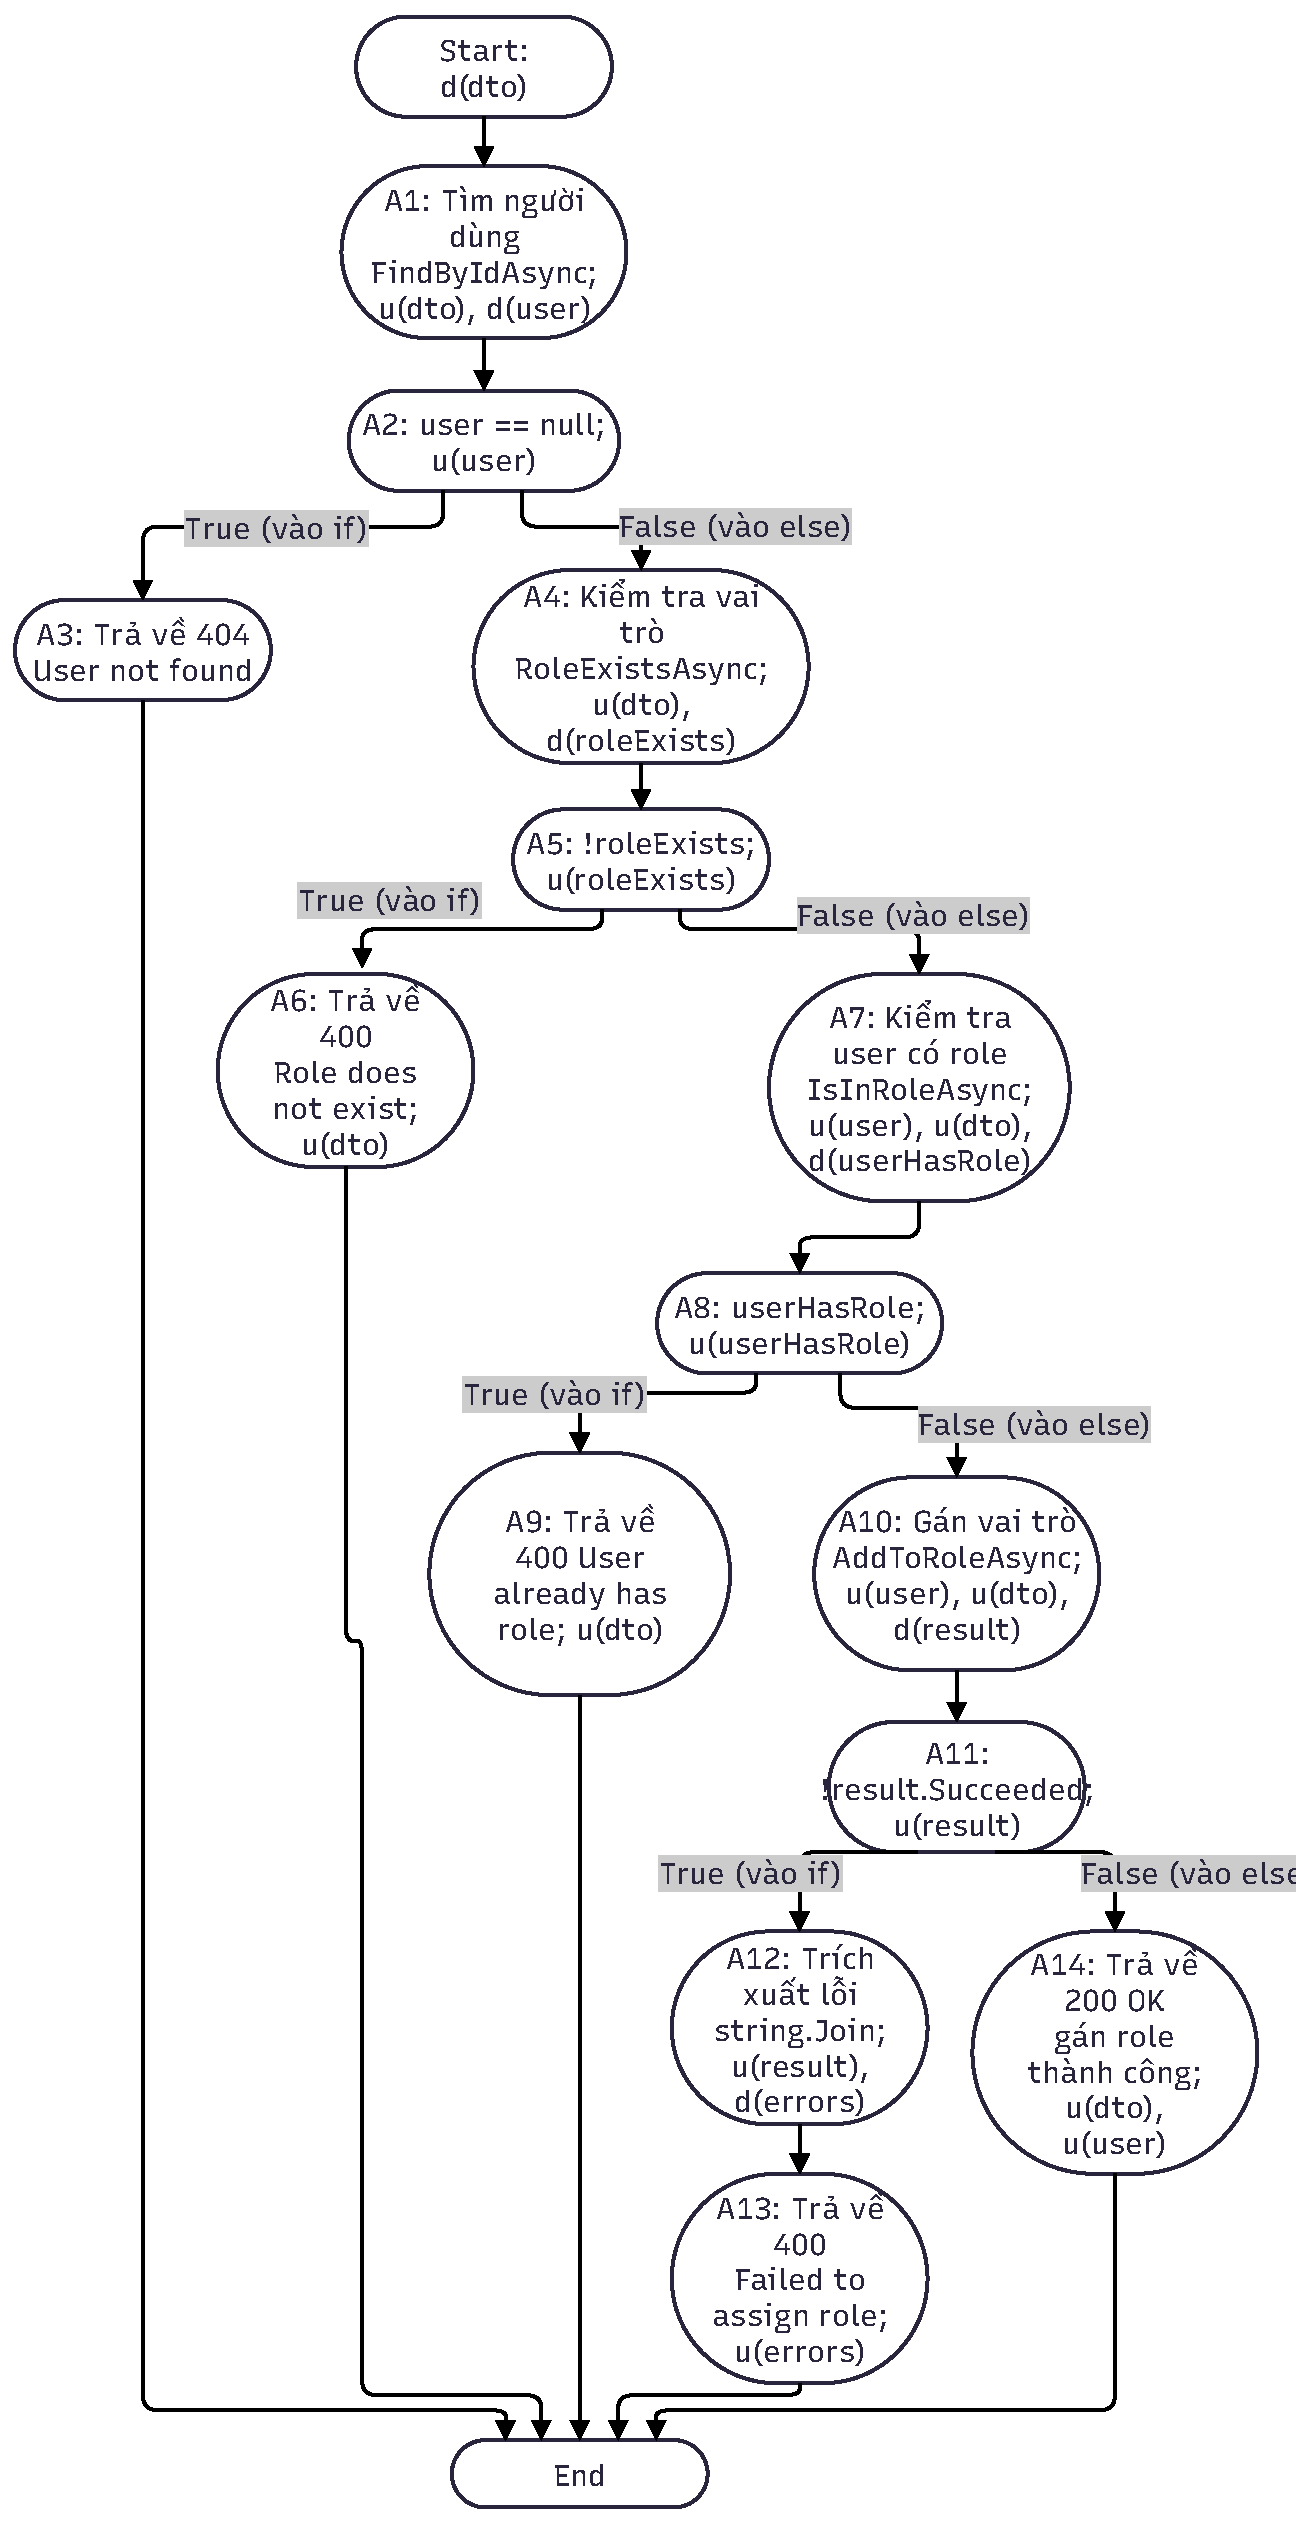
\includegraphics[width=0.92\textwidth,height=0.78\textheight,keepaspectratio]{AuthorizationDataFlow.pdf}
\caption{Đồ thị dòng dữ liệu (DFG) tổng hợp chức năng gán vai trò người dùng (\texttt{AssignRoleToUser})}
\end{figure}

\begin{itemize}[leftmargin=1.2cm, noitemsep]
    \item[\textbf{--}] \textbf{Thông số đồ thị:} Số nút $N = 16$ (\texttt{Start}, \texttt{End} và \texttt{A1}--\texttt{A14}), số cạnh $E = 19$, số nút quyết định $D = 4$ (\texttt{A2, A5, A8, A11}).
    \item[\textbf{--}] \textbf{Độ phức tạp Cyclomatic:} $M = V(G) = E - N + 2 = 19 - 16 + 2 = 5$ (kiểm tra đối chiếu: $V(G) = D + 1 = 4 + 1 = 5$).
    \item[\textbf{--}] \textbf{6 biến cần kiểm thử:} \texttt{dto}, \texttt{user}, \texttt{roleExists}, \texttt{userHasRole}, \texttt{result}, \texttt{errors}.
\end{itemize}

% Helper macro vẽ sơ đồ DFG thu gọn cho từng biến của AssignRoleToUser
\newcommand{\DrawAssignRoleVarDFG}{%
\begin{tikzpicture}[
    baseline=(S.north),
    >=Stealth,
    vnode/.style={circle, draw=black, minimum size=0.78cm, inner sep=0.5pt, font=\footnotesize\ttfamily\bfseries, align=center},
    startnode/.style={circle, draw=black, fill=green!70!teal, minimum size=0.30cm, inner sep=0pt},
    endnode/.style={circle, draw=black, double, fill=green!70!teal, minimum size=0.30cm, inner sep=0pt}
]
    \node[startnode] (S) at (0, 0) {};
    \node[vnode] (A1) at (0, -0.95) {\lblAone};
    \node[vnode] (A2) at (0, -2.25) {\lblAtwo};
    \node[vnode] (A3) at (-1.35, -3.45) {\lblAthree};
    \node[vnode] (A4) at (0.85, -3.45) {\lblAfour};
    \node[vnode] (A5) at (0.85, -5.25) {\lblAfive};
    \node[vnode] (A6) at (-0.50, -6.50) {\lblAsix};
    \node[vnode] (A7) at (1.95, -6.50) {\lblAseven};
    \node[vnode] (A8) at (1.95, -8.35) {\lblAeight};
    \node[vnode] (A9) at (0.60, -9.60) {\lblAnine};
    \node[vnode] (A10) at (3.05, -9.60) {\lblAten};
    \node[vnode] (A11) at (3.05, -10.95) {\lblAeleven};
    \node[vnode] (A12) at (2.00, -12.10) {\lblAtwelve};
    \node[vnode] (A13) at (2.00, -13.35) {\lblAthirteen};
    \node[vnode] (A14) at (4.00, -12.10) {\lblAfourteen};
    \node[endnode, label={[font=\footnotesize\ttfamily\bfseries, yshift=-2pt]below:k(all)}] (E) at (2.00, -14.45) {};

    \node[right=2pt of S, font=\footnotesize\ttfamily\bfseries] {\lblStart};

    \draw[->] (S) -- (A1);
    \draw[->] (A1) -- (A2);
    \draw[->] (A2) -| (A3);
    \draw[->] (A2) -| (A4);
    \draw[->] (A4) -- (A5);
    \draw[->] (A5) -| (A6);
    \draw[->] (A5) -| (A7);
    \draw[->] (A7) -- (A8);
    \draw[->] (A8) -| (A9);
    \draw[->] (A8) -| (A10);
    \draw[->] (A10) -- (A11);
    \draw[->] (A11) -| (A12);
    \draw[->] (A11) -| (A14);
    \draw[->] (A12) -- (A13);

    \draw[->] (A3) |- (E);
    \draw[->] (A6) |- (E);
    \draw[->] (A9) |- (E);
    \draw[->] (A13) -- (E);
    \draw[->] (A14) |- (E);
\end{tikzpicture}%
}

\noindent
\begin{minipage}[t]{0.485\textwidth}
\begin{tcolorbox}[colback=white, colframe=darkblue!35, boxrule=0.6pt, arc=2pt, left=4pt, right=4pt, top=4pt, bottom=4pt]
\begin{minipage}[t]{0.43\linewidth}
\scriptsize
\textbf{\textcolor{blue}{Kiểm thử biến \texttt{dto}}}\\[4pt]
\textbf{P1:} $\sim$duk\\
\textbf{P2:} $\sim$duuuk\\
\textbf{P3:} $\sim$duuuuk\\
\textbf{P4:} $\sim$duuuuk\\
\textbf{P5:} $\sim$duuuuuk\\[6pt]
\textbf{\textcolor{blue}{Kết luận:}}\\
Không có bất thường.
\end{minipage}\hfill
\begin{minipage}[t]{0.55\linewidth}
\centering
\def\lblStart{d(dto)}%
\def\lblAone{u(dto)}%
\def\lblAtwo{}%
\def\lblAthree{}%
\def\lblAfour{u(dto)}%
\def\lblAfive{}%
\def\lblAsix{u(dto)}%
\def\lblAseven{u(dto)}%
\def\lblAeight{}%
\def\lblAnine{u(dto)}%
\def\lblAten{u(dto)}%
\def\lblAeleven{}%
\def\lblAtwelve{}%
\def\lblAthirteen{}%
\def\lblAfourteen{u(dto)}%
\resizebox{\linewidth}{!}{\DrawAssignRoleVarDFG}
\end{minipage}
\end{tcolorbox}
\end{minipage}\hfill
\begin{minipage}[t]{0.485\textwidth}
\begin{tcolorbox}[colback=white, colframe=darkblue!35, boxrule=0.6pt, arc=2pt, left=4pt, right=4pt, top=4pt, bottom=4pt]
\begin{minipage}[t]{0.43\linewidth}
\scriptsize
\textbf{\textcolor{blue}{Kiểm thử biến \texttt{user}}}\\[4pt]
\textbf{P1:} $\sim$duk\\
\textbf{P2:} $\sim$duk\\
\textbf{P3:} $\sim$duuk\\
\textbf{P4:} $\sim$duuuk\\
\textbf{P5:} $\sim$duuuuk\\[6pt]
\textbf{\textcolor{blue}{Kết luận:}}\\
Không có bất thường.
\end{minipage}\hfill
\begin{minipage}[t]{0.55\linewidth}
\centering
\def\lblStart{}%
\def\lblAone{d(user)}%
\def\lblAtwo{u(user)}%
\def\lblAthree{}%
\def\lblAfour{}%
\def\lblAfive{}%
\def\lblAsix{}%
\def\lblAseven{u(user)}%
\def\lblAeight{}%
\def\lblAnine{}%
\def\lblAten{u(user)}%
\def\lblAeleven{}%
\def\lblAtwelve{}%
\def\lblAthirteen{}%
\def\lblAfourteen{u(user)}%
\resizebox{\linewidth}{!}{\DrawAssignRoleVarDFG}
\end{minipage}
\end{tcolorbox}
\end{minipage}

\vspace{4pt}
\noindent
\begin{minipage}[t]{0.485\textwidth}
\begin{tcolorbox}[colback=white, colframe=darkblue!35, boxrule=0.6pt, arc=2pt, left=4pt, right=4pt, top=4pt, bottom=4pt]
\begin{minipage}[t]{0.43\linewidth}
\scriptsize
\textbf{\textcolor{blue}{Kiểm thử biến \texttt{roleExists}}}\\[4pt]
\textbf{P1:} ---\\
\textbf{P2:} $\sim$duk\\
\textbf{P3:} $\sim$duk\\
\textbf{P4:} $\sim$duk\\
\textbf{P5:} $\sim$duk\\[6pt]
\textbf{\textcolor{blue}{Kết luận:}}\\
Không có bất thường.
\end{minipage}\hfill
\begin{minipage}[t]{0.55\linewidth}
\centering
\def\lblStart{}%
\def\lblAone{}%
\def\lblAtwo{}%
\def\lblAthree{}%
\def\lblAfour{d(role\\Exists)}%
\def\lblAfive{u(role\\Exists)}%
\def\lblAsix{}%
\def\lblAseven{}%
\def\lblAeight{}%
\def\lblAnine{}%
\def\lblAten{}%
\def\lblAeleven{}%
\def\lblAtwelve{}%
\def\lblAthirteen{}%
\def\lblAfourteen{}%
\resizebox{\linewidth}{!}{\DrawAssignRoleVarDFG}
\end{minipage}
\end{tcolorbox}
\end{minipage}\hfill
\begin{minipage}[t]{0.485\textwidth}
\begin{tcolorbox}[colback=white, colframe=darkblue!35, boxrule=0.6pt, arc=2pt, left=4pt, right=4pt, top=4pt, bottom=4pt]
\begin{minipage}[t]{0.43\linewidth}
\scriptsize
\textbf{\textcolor{blue}{Kiểm thử biến \texttt{userHasRole}}}\\[4pt]
\textbf{P1:} ---\\
\textbf{P2:} ---\\
\textbf{P3:} $\sim$duk\\
\textbf{P4:} $\sim$duk\\
\textbf{P5:} $\sim$duk\\[6pt]
\textbf{\textcolor{blue}{Kết luận:}}\\
Không có bất thường.
\end{minipage}\hfill
\begin{minipage}[t]{0.55\linewidth}
\centering
\def\lblStart{}%
\def\lblAone{}%
\def\lblAtwo{}%
\def\lblAthree{}%
\def\lblAfour{}%
\def\lblAfive{}%
\def\lblAsix{}%
\def\lblAseven{d(user\\HasRole)}%
\def\lblAeight{u(user\\HasRole)}%
\def\lblAnine{}%
\def\lblAten{}%
\def\lblAeleven{}%
\def\lblAtwelve{}%
\def\lblAthirteen{}%
\def\lblAfourteen{}%
\resizebox{\linewidth}{!}{\DrawAssignRoleVarDFG}
\end{minipage}
\end{tcolorbox}
\end{minipage}

\vspace{4pt}
\noindent
\begin{minipage}[t]{0.485\textwidth}
\begin{tcolorbox}[colback=white, colframe=darkblue!35, boxrule=0.6pt, arc=2pt, left=4pt, right=4pt, top=4pt, bottom=4pt]
\begin{minipage}[t]{0.43\linewidth}
\scriptsize
\textbf{\textcolor{blue}{Kiểm thử biến \texttt{result}}}\\[4pt]
\textbf{P1:} ---\\
\textbf{P2:} ---\\
\textbf{P3:} ---\\
\textbf{P4:} $\sim$duuk\\
\textbf{P5:} $\sim$duk\\[6pt]
\textbf{\textcolor{blue}{Kết luận:}}\\
Không có bất thường.
\end{minipage}\hfill
\begin{minipage}[t]{0.55\linewidth}
\centering
\def\lblStart{}%
\def\lblAone{}%
\def\lblAtwo{}%
\def\lblAthree{}%
\def\lblAfour{}%
\def\lblAfive{}%
\def\lblAsix{}%
\def\lblAseven{}%
\def\lblAeight{}%
\def\lblAnine{}%
\def\lblAten{d(res)}%
\def\lblAeleven{u(res)}%
\def\lblAtwelve{u(res)}%
\def\lblAthirteen{}%
\def\lblAfourteen{}%
\resizebox{\linewidth}{!}{\DrawAssignRoleVarDFG}
\end{minipage}
\end{tcolorbox}
\end{minipage}\hfill
\begin{minipage}[t]{0.485\textwidth}
\begin{tcolorbox}[colback=white, colframe=darkblue!35, boxrule=0.6pt, arc=2pt, left=4pt, right=4pt, top=4pt, bottom=4pt]
\begin{minipage}[t]{0.43\linewidth}
\scriptsize
\textbf{\textcolor{blue}{Kiểm thử biến \texttt{errors}}}\\[4pt]
\textbf{P1:} ---\\
\textbf{P2:} ---\\
\textbf{P3:} ---\\
\textbf{P4:} $\sim$duk\\
\textbf{P5:} ---\\[6pt]
\textbf{\textcolor{blue}{Kết luận:}}\\
Không có bất thường.
\end{minipage}\hfill
\begin{minipage}[t]{0.55\linewidth}
\centering
\def\lblStart{}%
\def\lblAone{}%
\def\lblAtwo{}%
\def\lblAthree{}%
\def\lblAfour{}%
\def\lblAfive{}%
\def\lblAsix{}%
\def\lblAseven{}%
\def\lblAeight{}%
\def\lblAnine{}%
\def\lblAten{}%
\def\lblAeleven{}%
\def\lblAtwelve{d(err)}%
\def\lblAthirteen{u(err)}%
\def\lblAfourteen{}%
\resizebox{\linewidth}{!}{\DrawAssignRoleVarDFG}
\end{minipage}
\end{tcolorbox}
\end{minipage}

\begin{table}[H]
\centering
\small
\begin{tabularx}{\textwidth}{|X|C{2.2cm}|C{2.2cm}|C{2.2cm}|C{2.2cm}|C{2.2cm}|}
\hline
\rowcolor[RGB]{179, 205, 255}
\textbf{Biến} & \textbf{P1} & \textbf{P2} & \textbf{P3} & \textbf{P4} & \textbf{P5} \tabularnewline
\hline
\texttt{dto} & $\sim$duk & $\sim$duuuk & $\sim$duuuuk & $\sim$duuuuk & $\sim$duuuuuk \\ \hline
\texttt{user} & $\sim$duk & $\sim$duk & $\sim$duuk & $\sim$duuuk & $\sim$duuuuk \\ \hline
\texttt{roleExists} & --- & $\sim$duk & $\sim$duk & $\sim$duk & $\sim$duk \\ \hline
\texttt{userHasRole} & --- & --- & $\sim$duk & $\sim$duk & $\sim$duk \\ \hline
\texttt{result} & --- & --- & --- & $\sim$duuk & $\sim$duk \\ \hline
\texttt{errors} & --- & --- & --- & $\sim$duk & --- \\ \hline
\end{tabularx}
\caption{Bảng tổng hợp chuỗi trạng thái \texttt{d/u/k} của 6 biến trên 5 đường độc lập \texttt{P1}--\texttt{P5}}
\end{table}

\noindent\textbf{e. Các đường độc lập (\texttt{P1}--\texttt{P5})}

\begin{table}[H]
\centering
\scriptsize
\setlength{\tabcolsep}{4pt}
\begin{tabularx}{\textwidth}{|C{1.1cm}|C{1.3cm}|X|L{4.2cm}|}
\hline
\rowcolor[RGB]{179, 205, 255}
\textbf{Đường} & \textbf{TC\#} & \textbf{Chuỗi nút trên đường độc lập (\texttt{A1}--\texttt{A14})} & \textbf{Kịch bản điều kiện} \tabularnewline
\hline
\textbf{P1} & TC 238 & $\text{Start} \rightarrow A1 \rightarrow A2\,(T) \rightarrow A3 \rightarrow \text{End}$ & Người dùng không tồn tại (HTTP 404) \\ \hline
\textbf{P2} & TC 239 & $\text{Start} \rightarrow A1 \rightarrow A2\,(F) \rightarrow A4 \rightarrow A5\,(T) \rightarrow A6 \rightarrow \text{End}$ & Vai trò không tồn tại (HTTP 400) \\ \hline
\textbf{P3} & TC 240 & $\text{Start} \rightarrow A1 \rightarrow A2\,(F) \rightarrow A4 \rightarrow A5\,(F) \rightarrow A7 \rightarrow A8\,(T) \rightarrow A9 \rightarrow \text{End}$ & Người dùng đã sở hữu vai trò (HTTP 400) \\ \hline
\textbf{P4} & TC 241 & $\text{Start} \rightarrow A1 \rightarrow A2\,(F) \rightarrow A4 \rightarrow A5\,(F) \rightarrow A7 \rightarrow A8\,(F) \rightarrow A10 \rightarrow A11\,(T) \rightarrow A12 \rightarrow A13 \rightarrow \text{End}$ & Identity gán vai trò thất bại (HTTP 400) \\ \hline
\textbf{P5} & TC 222 & $\text{Start} \rightarrow A1 \rightarrow A2\,(F) \rightarrow A4 \rightarrow A5\,(F) \rightarrow A7 \rightarrow A8\,(F) \rightarrow A10 \rightarrow A11\,(F) \rightarrow A14 \rightarrow \text{End}$ & Gán vai trò thành công (HTTP 200 OK) \\ \hline
\end{tabularx}
\caption{Định nghĩa 5 đường độc lập \texttt{P1}--\texttt{P5} trên đồ thị dòng dữ liệu \texttt{AssignRoleToUser} (B14)}
\end{table}

\noindent\textbf{f. Bảng Test Cases chi tiết chức năng B14 (\texttt{AssignRoleToUser}):}
\begingroup
\scriptsize
\setlength{\tabcolsep}{3pt}
\begin{longtable}{|C{0.8cm}|C{0.75cm}|C{0.95cm}|L{2.0cm}|L{3.0cm}|L{2.25cm}|L{2.6cm}|L{2.5cm}|C{0.85cm}|}
\hline
\rowcolor[RGB]{179, 205, 255}
\textbf{TC\#} & \textbf{BR\#} & \textbf{TR\#} & \textbf{TestCase} & \textbf{TestSteps} & \textbf{Test Data} & \textbf{Expected} & \textbf{Result} & \textbf{P/F} \tabularnewline
\hline
\endfirsthead
\hline
\rowcolor[RGB]{179, 205, 255}
\textbf{TC\#} & \textbf{BR\#} & \textbf{TR\#} & \textbf{TestCase} & \textbf{TestSteps} & \textbf{Test Data} & \textbf{Expected} & \textbf{Result} & \textbf{P/F} \tabularnewline
\hline
\endhead
\hline
\endfoot
\hline
\caption{Bảng Test Cases hộp trắng chức năng B14 -- AssignRoleToUser (Data Flow)}
\endlastfoot
\textbf{222} & B14 & T159, T167.1 & Gán vai trò cho người dùng thành công (P5) & 1. u1 hợp lệ, chưa có role Admin\newline 2. Gửi POST /api/admin/\allowbreak assign-role & UserId = ``u1\_id''\newline Role = ``Admin'' & HTTP 200 OK ``Role 'Admin' assigned to u1'', lưu vào DB. & HTTP 200 OK, gán quyền thành công. & \textcolor{blue}{\textbf{Pass}} \\ \hline
\textbf{238} & B14 & T167.1 & Từ chối gán vai trò khi user không tồn tại (P1) & 1. Chuẩn bị UserId không tồn tại\newline 2. Gửi POST /api/admin/\allowbreak assign-role & UserId = ``non\_\allowbreak existent''\newline Role = ``Admin'' & HTTP 404 Not Found với thông báo ``User not found''. & HTTP 404 Not Found, ``User not found''. & \textcolor{blue}{\textbf{Pass}} \\ \hline
\textbf{239} & B14 & T167.1 & Từ chối khi vai trò không tồn tại (P2) & 1. Chuẩn bị u1 tồn tại\newline 2. Gửi Role = ``SuperAdmin'' chưa tạo & UserId = ``u1\_id''\newline Role = ``SuperAdmin'' & HTTP 400 Bad Request ``Role 'SuperAdmin' does not exist''. & HTTP 400 Bad Request đúng thông báo. & \textcolor{blue}{\textbf{Pass}} \\ \hline
\textbf{240} & B14 & T167.1 & Từ chối khi người dùng đã sở hữu vai trò (P3) & 1. Chuẩn bị u1 đã có role Admin\newline 2. Gửi yêu cầu gán lại role Admin & UserId = ``u1\_id''\newline Role = ``Admin'' & HTTP 400 Bad Request ``User already has role 'Admin'''. & HTTP 400 Bad Request, không gọi gán lại. & \textcolor{blue}{\textbf{Pass}} \\ \hline
\textbf{241} & B14 & T167.1 & Báo lỗi khi Identity thực thi gán thất bại (P4) & 1. u1 chưa có role Moderator\newline 2. Giả lập AddToRoleAsync trả về lỗi DB & UserId = ``u1\_id''\newline Role = ``Moderator'' & HTTP 400 Bad Request ``Failed to assign role: Database failure''. & HTTP 400 Bad Request kèm chuỗi lỗi Identity. & \textcolor{blue}{\textbf{Pass}} \\ \hline
\end{longtable}
\endgroup


% ----------------------------------------------------------
% 4.3 White-box Coverage Testing
% ----------------------------------------------------------
\subsection{Kiểm thử mức độ bao phủ (White-box Coverage Testing)}

\subsubsection{Chức năng B4 -- Tạo bài viết (\texttt{PostsController.Create})}

\noindent\textbf{a. Mô tả nghiệp vụ \& Yêu cầu kỹ thuật (TRD)}
\begin{itemize}[leftmargin=1.2cm, noitemsep]
    \item[\textbf{--}] \textbf{Mã BRD:} B4.
    \item[\textbf{--}] \textbf{Tên chức năng:} Đăng bài viết trên bảng tin (\texttt{PostsController.Create}).
    \item[\textbf{--}] \textbf{Mục đích:} Cho phép người dùng tạo bài viết có nội dung văn bản, có thể đính kèm hình ảnh, và cập nhật bài viết đến người dùng khác theo thời gian thực.
    \item[\textbf{--}] \textbf{Tiền điều kiện của luồng thành công:} Người dùng đã đăng nhập; nội dung bài viết hợp lệ.
    \item[\textbf{--}] \textbf{Yêu cầu nghiệp vụ liên quan:}
    \begin{itemize}[leftmargin=0.8cm, label=$\bullet$, noitemsep]
        \item Người dùng phải được xác thực khi đăng bài.
        \item Nội dung không được để trống hoặc chỉ chứa khoảng trắng.
        \item Nội dung không được vượt quá 5.000 ký tự.
        \item Bài viết hợp lệ được lưu vào cơ sở dữ liệu.
        \item Sau khi đọc lại được bài viết vừa tạo, hệ thống phát sự kiện \texttt{PostCreated} đến nhóm \texttt{feed}.
        \item Nếu \texttt{SharedPostId = null}, hệ thống gọi dịch vụ thông báo bài viết mới đến bạn bè.
    \end{itemize}
\end{itemize}

\begin{table}[H]
\centering
\small
\begin{tabularx}{\textwidth}{|C{1.8cm}|X|}
\hline
\rowcolor[RGB]{179, 205, 255}
\textbf{Mã TRD} & \textbf{Mô tả yêu cầu} \tabularnewline
\hline
\textbf{T64} & Người dùng phải đăng nhập trước khi sử dụng chức năng đăng bài viết. \\ \hline
\textbf{T65} & Kiểm tra nội dung khi tạo bài viết; không cho phép đăng khi thiếu nội dung văn bản. \\ \hline
\textbf{T66} & Nội dung bài viết có độ dài từ 1 đến 5.000 ký tự. \\ \hline
\textbf{T66.1} & Khi không đọc lại được bài viết vừa tạo, hệ thống trả về HTTP 500 với thông báo ``Failed to retrieve created post''; không phát sự kiện \texttt{PostCreated} và không gửi thông báo bài viết mới. \\ \hline
\textbf{T71} & Đồng bộ bài viết mới trên bảng tin theo thời gian thực. \\ \hline
\textbf{T72} & Bạn bè nhận được thông báo khi người dùng đăng bài viết mới. \\ \hline
\end{tabularx}
\caption{Các yêu cầu TRD liên quan đến chức năng đăng bài viết (B4)}
\end{table}

\noindent\textbf{b. Mã nguồn đối tượng kiểm thử và danh mục vị trí câu lệnh (\texttt{S1}--\texttt{S16})}
\begin{lstlisting}[language={[Sharp]C}]
[HttpPost]
public async Task<IActionResult> Create([FromBody] CreatePostDto createPostDto)
{
    /* S1 */  var userId = User.FindFirst(ClaimTypes.NameIdentifier)?.Value;
    /* S2 */  if (string.IsNullOrEmpty(userId))
    /* S3 */      return this.UnauthorizedResponse("User not authenticated");
    /* S4 */  if (string.IsNullOrWhiteSpace(createPostDto.Content))
    /* S5 */      return this.BadRequestResponse(new List<ApiError> {
                      new ApiError("Content khong duoc de trong", "EMPTY_CONTENT") });
    /* S6 */  if (createPostDto.Content.Length > 5000)
    /* S7 */      return this.BadRequestResponse(new List<ApiError> {
                      new ApiError("Content khong duoc vuot qua 5000 ky tu", "CONTENT_TOO_LONG") });
    /* S8 */  var post = new Post {
                  Content = createPostDto.Content,
                  ImageUrl = await _imageStorage.SaveDataUriAsync(createPostDto.ImageUrl, "posts"),
                  UserId = userId, GroupId = null, SharedPostId = createPostDto.SharedPostId
              };
    /* S9 */  var created = await _postService.CreateAsync(post);
    /* S10 */ var createdWithUser = await _postService.GetByIdDtoAsync(created.Id);
    /* S11 */ if (createdWithUser == null)
    /* S12 */     return this.ErrorResponse("Failed to retrieve created post", statusCode: 500);
    /* S13 */ await _postHub.Clients.Group("feed").SendAsync("PostCreated", createdWithUser);
    /* S14 */ if (createdWithUser.SharedPostId == null)
    /* S15 */     await _notificationService.NotifyFriendsAboutNewPostAsync(userId, createdWithUser.Id);
    /* S16 */ return this.CreatedResponse(createdWithUser, "Post created successfully");
}
\end{lstlisting}

\begin{table}[H]
\centering
\scriptsize
\begin{tabularx}{\textwidth}{|C{1.3cm}|X|L{4.0cm}|}
\hline
\rowcolor[RGB]{179, 205, 255}
\textbf{Nhãn} & \textbf{Nội dung} & \textbf{Vai trò} \tabularnewline
\hline
\textbf{S1} & Lấy mã người dùng từ thông tin xác thực & Xác định người đăng \\ \hline
\textbf{S2} & Kiểm tra mã người dùng rỗng & Quyết định 1 \\ \hline
\textbf{S3} & Trả về HTTP 401 & Kết thúc sớm \\ \hline
\textbf{S4} & Kiểm tra nội dung rỗng hoặc chỉ chứa khoảng trắng & Quyết định 2 \\ \hline
\textbf{S5} & Trả về HTTP 400 do thiếu nội dung & Kết thúc sớm \\ \hline
\textbf{S6} & Kiểm tra nội dung vượt 5.000 ký tự & Quyết định 3 \\ \hline
\textbf{S7} & Trả về HTTP 400 do vượt độ dài & Kết thúc sớm \\ \hline
\textbf{S8} & Khởi tạo bài viết và xử lý ảnh & Bước xử lý \\ \hline
\textbf{S9} & Lưu bài viết & Bước xử lý \\ \hline
\textbf{S10} & Đọc lại bài viết vừa tạo & Bước xử lý \\ \hline
\textbf{S11} & Kiểm tra kết quả đọc lại bằng \texttt{null} & Quyết định 4 \\ \hline
\textbf{S12} & Trả về HTTP 500 & Kết thúc sớm \\ \hline
\textbf{S13} & Phát sự kiện \texttt{PostCreated} đến \texttt{feed} & Bước xử lý \\ \hline
\textbf{S14} & Kiểm tra \texttt{SharedPostId == null} & Quyết định 5 \\ \hline
\textbf{S15} & Gọi dịch vụ thông báo bài viết mới & Nhánh True của \texttt{S14} \\ \hline
\textbf{S16} & Trả về HTTP 201 & Kết thúc thành công \\ \hline
\end{tabularx}
\caption{Danh mục 16 vị trí câu lệnh dùng để tính bao phủ (\texttt{PostsController.Create} -- B4)}
\end{table}

\noindent\textbf{c. Đồ thị dòng điều khiển (CFG) và quy ước các nhánh (\texttt{B1}--\texttt{B10})}
\begin{figure}[H]
\centering
\begin{tikzpicture}[
    scale=0.92, transform shape,
    >=Stealth,
    proc/.style={rectangle, rounded corners=3pt, draw=darkblue, fill=blue!6, minimum width=2.4cm, minimum height=0.55cm, align=center, font=\scriptsize},
    dec/.style={rectangle, rounded corners=6pt, draw=primaryblue, fill=blue!12, minimum width=2.5cm, minimum height=0.58cm, align=center, font=\scriptsize\bfseries},
    term/.style={circle, draw=darkblue, fill=green!15, minimum size=0.65cm, font=\scriptsize\bfseries},
    lbl/.style={font=\tiny\bfseries, fill=white, inner sep=1pt}
]
    \node[term] (Start) at (0, 0) {Start};
    \node[proc] (S1) at (0, -0.95) {\textbf{S1:} Lấy \texttt{userId}};
    \node[dec] (S2) at (0, -1.95) {\textbf{S2:} \texttt{userId} rỗng};

    \node[proc] (S3) at (-3.6, -3.15) {\textbf{S3:} Trả về 401\\Unauthorized};
    \node[dec] (S4) at (2.1, -3.15) {\textbf{S4:} \texttt{Content} rỗng /\\khoảng trắng};

    \node[proc] (S5) at (-1.5, -4.55) {\textbf{S5:} Trả về 400\\Thiếu nội dung};
    \node[dec] (S6) at (4.4, -4.55) {\textbf{S6:} \texttt{Content.Length}\\$> 5000$};

    \node[proc] (S7) at (0.8, -5.95) {\textbf{S7:} Trả về 400\\Nội dung quá dài};
    \node[proc] (S8) at (6.4, -5.95) {\textbf{S8:} Khởi tạo \texttt{post},\\\texttt{GroupId = null}};
    \node[proc] (S9) at (6.4, -7.05) {\textbf{S9:} Lưu bài viết};
    \node[proc] (S10) at (6.4, -8.00) {\textbf{S10:} Đọc lại bài viết};
    \node[dec] (S11) at (6.4, -9.05) {\textbf{S11:} \texttt{createdWithUser}\\$==$ \texttt{null}};

    \node[proc] (S12) at (3.2, -10.35) {\textbf{S12:} Trả về 500};
    \node[proc] (S13) at (8.2, -10.35) {\textbf{S13:} Phát \texttt{PostCreated}\\đến \texttt{feed}};
    \node[dec] (S14) at (8.2, -11.45) {\textbf{S14:} \texttt{SharedPostId}\\$==$ \texttt{null}};

    \node[proc] (S15) at (5.6, -12.65) {\textbf{S15:} Gọi dịch vụ\\thông báo};
    \node[proc] (S16) at (8.2, -13.75) {\textbf{S16:} Trả về 201\\Created};
    \coordinate (Merge) at (1.8, -14.55);
    \node[term] (End) at (1.8, -15.30) {End};

    \draw[->] (Start) -- (S1);
    \draw[->] (S1) -- (S2);
    \draw[->] (S2) -| node[lbl, pos=0.78] {B1 (True)} (S3);
    \draw[->] (S2) -| node[lbl, pos=0.78] {B2 (False)} (S4);
    \draw[->] (S4) -| node[lbl, pos=0.78] {B3 (True)} (S5);
    \draw[->] (S4) -| node[lbl, pos=0.78] {B4 (False)} (S6);
    \draw[->] (S6) -| node[lbl, pos=0.78] {B5 (True)} (S7);
    \draw[->] (S6) -| node[lbl, pos=0.78] {B6 (False)} (S8);
    \draw[->] (S8) -- (S9);
    \draw[->] (S9) -- (S10);
    \draw[->] (S10) -- (S11);
    \draw[->] (S11) -| node[lbl, pos=0.78] {B7 (True)} (S12);
    \draw[->] (S11) -| node[lbl, pos=0.78] {B8 (False)} (S13);
    \draw[->] (S13) -- (S14);
    \draw[->] (S14) -| node[lbl, pos=0.78] {B9 (True)} (S15);
    \draw[->] (S14) -- node[lbl, pos=0.5, right] {B10 (False)} (S16);
    \draw[->] (S15) |- (S16);

    \draw (S3) |- (Merge);
    \draw (S5) |- (Merge);
    \draw (S7) |- (Merge);
    \draw (S12) |- (Merge);
    \draw (S16) |- (Merge);
    \draw[->] (Merge) -- (End);
\end{tikzpicture}
\caption{Đồ thị dòng điều khiển (CFG) chức năng đăng bài viết (\texttt{PostsController.Create})}
\end{figure}

\begin{table}[H]
\centering
\small
\begin{tabularx}{\textwidth}{|C{2.0cm}|X|C{3.0cm}|C{3.0cm}|}
\hline
\rowcolor[RGB]{179, 205, 255}
\textbf{Quyết định} & \textbf{Điều kiện} & \textbf{Nhánh True} & \textbf{Nhánh False} \tabularnewline
\hline
\textbf{S2} & \texttt{string.IsNullOrEmpty(userId)} & B1: đến S3 & B2: đến S4 \\ \hline
\textbf{S4} & \texttt{string.IsNullOrWhiteSpace(Content)} & B3: đến S5 & B4: đến S6 \\ \hline
\textbf{S6} & \texttt{Content.Length > 5000} & B5: đến S7 & B6: đến S8 \\ \hline
\textbf{S11} & \texttt{createdWithUser == null} & B7: đến S12 & B8: đến S13 \\ \hline
\textbf{S14} & \texttt{createdWithUser.SharedPostId == null} & B9: đến S15 & B10: đến S16 \\ \hline
\end{tabularx}
\caption{Các nhánh kết quả của năm quyết định (\texttt{PostsController.Create} -- B4)}
\end{table}

\noindent\textbf{d. Độ phức tạp Cyclomatic và Sáu đường đi độc lập cơ bản (\texttt{P1}--\texttt{P6}):}
\begin{itemize}[leftmargin=1.2cm, noitemsep]
    \item[\textbf{--}] \textbf{Đồ thị dòng điều khiển gồm:} Số nút $N = 18$ (\texttt{Start}, \texttt{End} và 16 vị trí câu lệnh \texttt{S1}--\texttt{S16}), số cạnh $E = 22$, số nút quyết định $D = 5$ (\texttt{S2, S4, S6, S11, S14}).
    \item[\textbf{--}] \textbf{Độ phức tạp Cyclomatic:} $V(G) = E - N + 2 = 22 - 18 + 2 = 6$ (kiểm tra: $V(G) = D + 1 = 5 + 1 = 6$).
\end{itemize}
\begin{table}[H]
\centering
\small
\begin{tabularx}{\textwidth}{|C{1.3cm}|L{7.8cm}|X|}
\hline
\rowcolor[RGB]{179, 205, 255}
\textbf{Đường} & \textbf{Chuỗi nút thực thi} & \textbf{Ý nghĩa nghiệp vụ} \tabularnewline
\hline
\textbf{P1} & \texttt{Start} $\rightarrow$ S1 $\rightarrow$ S2 $\rightarrow$ S3 $\rightarrow$ \texttt{End} & Không xác định được người dùng (401 Unauthorized). \\ \hline
\textbf{P2} & \texttt{Start} $\rightarrow$ S1 $\rightarrow$ S2 $\rightarrow$ S4 $\rightarrow$ S5 $\rightarrow$ \texttt{End} & Nội dung bài viết rỗng (400 Bad Request). \\ \hline
\textbf{P3} & \texttt{Start} $\rightarrow$ S1 $\rightarrow$ S2 $\rightarrow$ S4 $\rightarrow$ S6 $\rightarrow$ S7 $\rightarrow$ \texttt{End} & Nội dung vượt 5.000 ký tự (400 Bad Request). \\ \hline
\textbf{P4} & \texttt{Start} $\rightarrow$ S1 $\rightarrow$ S2 $\rightarrow$ S4 $\rightarrow$ S6 $\rightarrow$ S8 $\rightarrow$ S9 $\rightarrow$ S10 $\rightarrow$ S11 $\rightarrow$ S12 $\rightarrow$ \texttt{End} & Đã gọi lưu bài nhưng không đọc lại được kết quả (500 Error). \\ \hline
\textbf{P5} & \texttt{Start} $\rightarrow$ S1 $\rightarrow$ S2 $\rightarrow$ S4 $\rightarrow$ S6 $\rightarrow$ S8 $\rightarrow$ S9 $\rightarrow$ S10 $\rightarrow$ S11 $\rightarrow$ S13 $\rightarrow$ S14 $\rightarrow$ S15 $\rightarrow$ S16 $\rightarrow$ \texttt{End} & Tạo bài gốc thành công, phát SignalR và gọi thông báo bạn bè. \\ \hline
\textbf{P6} & \texttt{Start} $\rightarrow$ S1 $\rightarrow$ S2 $\rightarrow$ S4 $\rightarrow$ S6 $\rightarrow$ S8 $\rightarrow$ S9 $\rightarrow$ S10 $\rightarrow$ S11 $\rightarrow$ S13 $\rightarrow$ S14 $\rightarrow$ S16 $\rightarrow$ \texttt{End} & Tạo bài có tham chiếu bài gốc (\texttt{SharedPostId != null}), bỏ qua S15. \\ \hline
\end{tabularx}
\caption{Sáu đường độc lập cơ bản của \texttt{PostsController.Create} (B4)}
\end{table}

\noindent\textbf{e. Phân tích các mức độ bao phủ}

\noindent\textbf{e.1 Bao phủ câu lệnh -- Statement Coverage}

\noindent Bao phủ câu lệnh được tính bằng số vị trí S1--S16 đã được thực thi ít nhất một lần trên tổng số 16 vị trí đã xác định:
\[
\text{Statement Coverage} = \frac{\text{Số vị trí câu lệnh đã thực thi}}{16} \times 100\%.
\]
Tỉ lệ tích lũy được tính theo hợp các câu lệnh đã đi qua, không cộng lặp câu lệnh giữa các TC.

\begin{table}[H]
\centering
\scriptsize
\begin{tabularx}{\textwidth}{|L{2.2cm}|C{1.1cm}|X|C{1.2cm}|C{1.4cm}|C{1.4cm}|C{1.6cm}|}
\hline
\rowcolor[RGB]{179, 205, 255}
\textbf{Mã TC} & \textbf{Đường} & \textbf{Các câu lệnh thực thi} & \textbf{Số lệnh} & \textbf{Đơn lẻ}  \tabularnewline
\hline
COV-POST-01 & P1 & S1, S2, S3 & 3 & 18,75\%  \\ \hline
COV-POST-02 & P2 & S1, S2, S4, S5 & 4 & 25,00\%  \\ \hline
COV-POST-03 & P3 & S1, S2, S4, S6, S7 & 5 & 31,25\% \\ \hline
COV-POST-04 & P4 & S1, S2, S4, S6, S8, S9, S10, S11, S12 & 9 & 56,25\%  \\ \hline
COV-POST-05 & P5 & S1, S2, S4, S6, S8, S9, S10, S11, S13, S14, S15, S16 & 12 & 75,00\%  \\ \hline
COV-POST-06 & P6 & S1, S2, S4, S6, S8, S9, S10, S11, S13, S14, S16 & 11 & 68,75\%  \\ \hline
\end{tabularx}
\caption{Ma trận bao phủ câu lệnh lũy tiến (\texttt{PostsController.Create} -- B4)}
\end{table}

\noindent\textit{Nhận xét:} Sau TC05, tập đường đã đi qua đủ 16 vị trí câu lệnh. TC06 không bổ sung câu lệnh mới nhưng cần thiết để kiểm tra nhánh False của S14.

\noindent\textbf{e.2 Bao phủ nhánh/quyết định (Branch/Decision Coverage)}

\noindent Trong mô hình này, nhánh được đếm là hai kết quả True/False của mỗi câu lệnh \texttt{if}. Có năm quyết định, tương ứng 10 nhánh kết quả:
\[
\text{Branch Coverage} = \frac{\text{Số nhánh kết quả đã thực thi}}{10} \times 100\%.
\]

\begin{table}[H]
\centering
\scriptsize
\begin{tabularx}{\textwidth}{|L{2.2cm}|C{1.1cm}|X|L{2.3cm}|C{1.4cm}|C{2.4cm}|}
\hline
\rowcolor[RGB]{179, 205, 255}
\textbf{Mã TC} & \textbf{Đường} & \textbf{Các nhánh thực thi} & \textbf{Nhánh bổ sung} & \textbf{Đơn lẻ} & \textbf{Tích lũy} \tabularnewline
\hline
COV-POST-01 & P1 & B1 & B1 & 10,00\% & 10,00\% -- 1/10 \\ \hline
COV-POST-02 & P2 & B2, B3 & B2, B3 & 20,00\% & 30,00\% -- 3/10 \\ \hline
COV-POST-03 & P3 & B2, B4, B5 & B4, B5 & 30,00\% & 50,00\% -- 5/10 \\ \hline
COV-POST-04 & P4 & B2, B4, B6, B7 & B6, B7 & 40,00\% & 70,00\% -- 7/10 \\ \hline
COV-POST-05 & P5 & B2, B4, B6, B8, B9 & B8, B9 & 50,00\% & 90,00\% -- 9/10 \\ \hline
COV-POST-06 & P6 & B2, B4, B6, B8, B10 & B10 & 50,00\% & 100,00\% -- 10/10 \\ \hline
\end{tabularx}
\caption{Ma trận bao phủ nhánh lũy tiến (\texttt{PostsController.Create} -- B4)}
\end{table}

\noindent\textit{Nhận xét:} Sáu TC được thiết kế để đi qua đủ cả hai kết quả của năm quyết định.

\noindent\textbf{e.3 Bao phủ điều kiện -- Condition Coverage}

\noindent Mỗi câu lệnh \texttt{if} trong đoạn mã chứa một điều kiện đơn. Vì vậy, trong phạm vi các điều kiện này, bao phủ điều kiện trùng với bao phủ quyết định. Dấu ``---'' biểu thị điều kiện không được đánh giá vì hàm đã kết thúc trước đó.

\begin{table}[H]
\centering
\small
\begin{tabularx}{\textwidth}{|L{2.5cm}|C{2.1cm}|C{2.1cm}|C{2.3cm}|C{2.4cm}|X|}
\hline
\rowcolor[RGB]{179, 205, 255}
\textbf{Mã TC} & \textbf{S2: userId rỗng} & \textbf{S4: Nội dung rỗng} & \textbf{S6: Dài quá 5000} & \textbf{S11: Đọc lại bằng null} & \textbf{S14: SharedPostId null} \tabularnewline
\hline
COV-POST-01 & True & --- & --- & --- & --- \\ \hline
COV-POST-02 & False & True & --- & --- & --- \\ \hline
COV-POST-03 & False & False & True & --- & --- \\ \hline
COV-POST-04 & False & False & False & True & --- \\ \hline
COV-POST-05 & False & False & False & False & True \\ \hline
COV-POST-06 & False & False & False & False & False \\ \hline
\end{tabularx}
\caption{Ma trận đánh giá các điều kiện đơn (\texttt{PostsController.Create} -- B4)}
\end{table}

\noindent Nếu thực thi đúng các đường đã thiết kế, mỗi điều kiện đều được đánh giá với cả True và False:
\[
\text{Condition Coverage} = \frac{10}{10} \times 100\% = 100\%.
\]

\noindent\textbf{e.4 Bao phủ đường đi -- Path Coverage}

\noindent Trong phạm vi đồ thị đã xác định, có sáu đường khả thi P1--P6:
\[
\text{Path Coverage} = \frac{\text{Số đường đã thực thi}}{\text{Tổng số đường khả thi trong mô hình}} \times 100\%.
\]

\noindent\textbf{Ghi chú phân tích kết quả kiểm thử:}
\begin{itemize}[leftmargin=1.2cm, noitemsep]
    \item[\textbf{--}] \textbf{\texttt{COV-POST-01} (P1):} Kiểm tra khả năng chặn truy cập khi chưa xác thực; đạt 18,75\% bao phủ câu lệnh và 10,00\% bao phủ nhánh.
    \item[\textbf{--}] \textbf{\texttt{COV-POST-02} (P2):} Kiểm thử ràng buộc dữ liệu đầu vào khi nội dung rỗng; tích lũy đạt 31,25\% câu lệnh và 30,00\% nhánh.
    \item[\textbf{--}] \textbf{\texttt{COV-POST-03} (P3):} Kiểm thử giới hạn độ dài nội dung tối đa 5.000 ký tự (\texttt{T66}); tích lũy đạt 43,75\% câu lệnh và 50,00\% nhánh.
    \item[\textbf{--}] \textbf{\texttt{COV-POST-04} (P4):} Kiểm thử ngoại lệ kỹ thuật khi không thể đọc lại bài viết vừa tạo sau lệnh lưu; tích lũy đạt 75,00\% câu lệnh và 70,00\% nhánh.
    \item[\textbf{--}] \textbf{\texttt{COV-POST-05} \& \texttt{COV-POST-06} (P5, P6):} Kiểm tra hai luồng xử lý thành công chính. \texttt{P5} đại diện cho bài viết gốc (gọi thông báo bạn bè, đưa bao phủ câu lệnh lên 100,00\% và nhánh lên 90,00\%). \texttt{P6} đại diện cho bài chia sẻ (bỏ qua thông báo bạn bè, hoàn tất 100,00\% bao phủ nhánh và 100,00\% bao phủ đường đi).
\end{itemize}

\noindent\textbf{f. Bảng Test Cases chi tiết chức năng B4 (\texttt{PostsController.Create}):}
\begingroup
\scriptsize
\setlength{\tabcolsep}{3pt}
\begin{longtable}{|C{0.8cm}|C{0.75cm}|C{0.95cm}|L{2.0cm}|L{3.0cm}|L{2.25cm}|L{2.6cm}|L{2.5cm}|C{0.85cm}|}
\hline
\rowcolor[RGB]{179, 205, 255}
\textbf{TC\#} & \textbf{BR\#} & \textbf{TR\#} & \textbf{TestCase} & \textbf{TestSteps} & \textbf{Test Data} & \textbf{Expected} & \textbf{Result} & \textbf{P/F} \tabularnewline
\hline
\endfirsthead
\hline
\rowcolor[RGB]{179, 205, 255}
\textbf{TC\#} & \textbf{BR\#} & \textbf{TR\#} & \textbf{TestCase} & \textbf{TestSteps} & \textbf{Test Data} & \textbf{Expected} & \textbf{Result} & \textbf{P/F} \tabularnewline
\hline
\endhead
\hline
\endfoot
\hline
\caption{Bảng Test Cases kiểm thử mức độ bao phủ chức năng B4 -- PostsController.Create}
\endlastfoot
\textbf{56} & B4 & T64 & Từ chối khi không xác định được người dùng (P1) & 1. Không cung cấp claim userId\newline 2. Gọi PostsController.\allowbreak Create & userId = null\newline Content = ``Bài thử'' & HTTP 401 Unauthorized ``User not authenticated''. & HTTP 401, đạt 18,75\% Stmt, 10,00\% Branch. & \textcolor{blue}{\textbf{Pass}} \\ \hline
\textbf{57} & B4 & T65 & Từ chối khi nội dung bài viết rỗng (P2) & 1. Thiết lập userId = ``u1''\newline 2. Đặt Content = ``'' và gọi Create & userId = ``u1''\newline Content = ``'' & HTTP 400 BadRequest ``Content không được để trống''. & HTTP 400, tích lũy 31,25\% Stmt, 30,00\% Branch. & \textcolor{blue}{\textbf{Pass}} \\ \hline
\textbf{77} & B4 & T65, T71 & Tạo bài gốc thành công và thông báo bạn bè (P5) & 1. Thiết lập SharedPostId = null\newline 2. Gọi Create và kiểm tra SignalR & userId = ``u1'', Content = ``Hợp lệ'', SharedPostId = null & HTTP 201 Created, phát PostCreated và gọi NotifyFriends 1 lần. & HTTP 201, tích lũy 100\% Stmt, 90,00\% Branch. & \textcolor{blue}{\textbf{Pass}} \\ \hline
\textbf{242} & B4 & T66.1 & Trả lỗi khi không đọc lại được bài vừa tạo (P4) & 1. Mock CreateAsync trả Id = 20\newline 2. Mock GetByIdDto\allowbreak Async(20) trả null & userId = ``u1''\newline GetByIdDto\allowbreak Async $\rightarrow$ null & HTTP 500 Internal Server Error ``Failed to retrieve created post''. & HTTP 500, tích lũy 75,00\% Stmt, 70,00\% Branch. & \textcolor{blue}{\textbf{Pass}} \\ \hline
\textbf{243} & B4 & T65, T71 & Tạo bài chia sẻ thành công, bỏ qua thông báo bạn bè (P6) & 1. Thiết lập SharedPostId = 10\newline 2. Gọi Create và kiểm tra & userId = ``u1'', Content = ``Share'', SharedPostId = 10 & HTTP 201 Created, phát PostCreated, không gọi NotifyFriends. & HTTP 201, hoàn tất 100\% Stmt \& 100\% Branch. & \textcolor{blue}{\textbf{Pass}} \\ \hline
\textbf{246} & B4 & T66 & Từ chối khi nội dung vượt 5000 ký tự (P3 -- Unit Test) & 1. Thiết lập userId = ``u1''\newline 2. Đặt Content = 5001 ký tự 'a', gọi Create & userId = ``u1''\newline Content = 5001 chars & HTTP 400 BadRequest ``Content không được vượt quá 5000 ký tự''. & HTTP 400, tích lũy 43,75\% Stmt, 50,00\% Branch. & \textcolor{blue}{\textbf{Pass}} \\ \hline
\end{longtable}
\endgroup

\noindent\textit{Ghi chú đối chiếu hộp trắng -- hộp đen:} Ca kiểm thử đơn vị \texttt{TC 246} (\texttt{COV-POST-03}) kiểm tra trực tiếp nhánh \texttt{S6} (\texttt{Content.Length > 5000}) của \texttt{PostsController.Create} ở cấp Unit Test và đạt \texttt{Pass}. Kết quả này tách biệt với ca kiểm thử hệ thống hộp đen \texttt{TC 64} ở Mục 3.7.1 (\texttt{Fail -- Defect \#1} trên giao diện phiên bản \texttt{v1.0}), cho thấy tồn tại sự mất đồng bộ giữa tầng giao diện/luồng tích hợp bản \texttt{v1.0} và điều kiện kiểm tra tại Controller, cần được kiểm tra tích hợp và chạy lại (Retesting) sau khi đồng bộ mã nguồn.

\subsubsection{Chức năng B8 -- Nhắn tin tức thời 1-1 (\texttt{SendPersonalMessageAsync})}

\noindent\textbf{a. Mô tả nghiệp vụ \& Yêu cầu kỹ thuật (TRD)}
\begin{itemize}[leftmargin=1.2cm, noitemsep]
    \item[\textbf{--}] \textbf{Mã BRD:} B8.
    \item[\textbf{--}] \textbf{Tên chức năng:} Gửi tin nhắn cá nhân 1-1 (\texttt{SendPersonalMessageAsync}).
    \item[\textbf{--}] \textbf{Mục đích:} Cho phép người dùng gửi tin nhắn văn bản hoặc hình ảnh đến một người dùng khác trong hệ thống theo thời gian thực qua giao thức SignalR.
    \item[\textbf{--}] \textbf{Tiền điều kiện:} Người gửi đã đăng nhập vào hệ thống và xác định được người nhận tin nhắn.
    \item[\textbf{--}] \textbf{Yêu cầu nghiệp vụ liên quan:}
    \begin{itemize}[leftmargin=0.8cm, label=$\bullet$, noitemsep]
        \item Mã người nhận (\texttt{receiverId}) không được để trống khi gửi tin nhắn cá nhân.
        \item Người dùng không được gửi tin nhắn khi cả nội dung văn bản và hình ảnh đều để trống.
        \item Độ dài nội dung văn bản của một tin nhắn không được vượt quá 2.000 ký tự.
        \item Hệ thống hỗ trợ xử lý và lưu trữ tệp hình ảnh đính kèm (nếu có).
        \item Khi gửi tin nhắn hợp lệ, hệ thống lưu bản ghi tin nhắn vào cơ sở dữ liệu, kích hoạt gửi thông báo đến người nhận và phát sóng sự kiện thời gian thực qua SignalR.
    \end{itemize}
\end{itemize}

\begin{table}[H]
\centering
\small
\begin{tabularx}{\textwidth}{|C{1.8cm}|X|}
\hline
\rowcolor[RGB]{179, 205, 255}
\textbf{Mã TRD} & \textbf{Mô tả yêu cầu} \tabularnewline
\hline
\textbf{T108} & Nội dung tin nhắn văn bản không được để trống hoặc chỉ chứa khoảng trắng nếu không gửi kèm tệp hình ảnh; nếu vi phạm Backend từ chối xử lý và ném ngoại lệ hoặc trả về lỗi HTTP 400 Bad Request. \\ \hline
\textbf{T109} & Độ dài nội dung văn bản của một tin nhắn không được vượt quá 2.000 ký tự; nếu vượt quá Backend từ chối xử lý và ném ngoại lệ hoặc trả về lỗi HTTP 400 Bad Request. \\ \hline
\textbf{T110} & Hỗ trợ gửi kèm tệp hình ảnh hợp lệ với dung lượng không vượt quá 5MB và lưu trữ an toàn vào hệ thống tệp. \\ \hline
\textbf{T111} & Hệ thống sử dụng kết nối SignalR để truyền nhận tin nhắn theo thời gian thực (sự kiện \texttt{ReceiveMessage}) đến người nhận ngay khi tin nhắn được tạo thành công. \\ \hline
\textbf{T114.1} & Chặn gửi tin nhắn cá nhân ở tầng dịch vụ khi thiếu thông tin người nhận (\texttt{receiverId} \texttt{null} hoặc rỗng); phương thức \texttt{SendPersonalMessageAsync} ném ngoại lệ \texttt{ArgumentException}. \\ \hline
\end{tabularx}
\caption{Bảng mô tả các yêu cầu kỹ thuật (TRD) liên quan đến chức năng gửi tin nhắn cá nhân (B8)}
\end{table}

\noindent\textbf{b. Mã nguồn đối tượng kiểm thử và danh mục vị trí câu lệnh (\texttt{S1}--\texttt{S14})}
\begin{lstlisting}[language={[Sharp]C}]
public async Task<Message> SendPersonalMessageAsync(
    string senderId, string receiverId, string content, string? imageUrl)
{
S1:  if (string.IsNullOrEmpty(receiverId))
     {
S2:      throw new ArgumentException("Ma nguoi nhan khong duoc de trong", nameof(receiverId));
     }
     else
     {
S3:      if (string.IsNullOrWhiteSpace(content) && string.IsNullOrWhiteSpace(imageUrl))
         {
S4:          throw new InvalidOperationException("Noi dung tin nhan hoac hinh anh khong duoc de trong");
         }
         else
         {
S5:          if (content != null && content.Length > 2000)
             {
S6:              throw new ArgumentException("Noi dung tin nhan khong duoc vuot qua 2000 ky tu", nameof(content));
             }
             else
             {
S7:              string? savedImageUrl = null;
S8:              if (!string.IsNullOrWhiteSpace(imageUrl))
                 {
S9:                  savedImageUrl = await _imageStorage.SaveDataUriAsync(imageUrl, "messages");
                 }
S10:             var message = new Message
                 {
                     SenderId = senderId, ReceiverId = receiverId,
                     Content = content?.Trim() ?? string.Empty,
                     ImageUrl = savedImageUrl, CreatedAt = DateTime.UtcNow, IsRead = false
                 };
S11:             await _messageService.CreateAsync(message);
S12:             await _notificationService.NotifyMessageAsync(receiverId, senderId,
                     message.Id, string.IsNullOrEmpty(message.Content) ? "[Hinh anh]" : message.Content);
S13:             await _messageHubContext.Clients.Group($"user_{receiverId}")
                     .SendAsync("ReceiveMessage", message);
S14:             return message;
             }
         }
     }
}
\end{lstlisting}

\begin{table}[H]
\centering
\scriptsize
\begin{tabularx}{\textwidth}{|C{1.4cm}|L{6.2cm}|X|}
\hline
\rowcolor[RGB]{179, 205, 255}
\textbf{Mã lệnh} & \textbf{Nội dung câu lệnh trong mã nguồn} & \textbf{Vai trò cú pháp} \tabularnewline
\hline
\textbf{S1} & \texttt{if (string.IsNullOrEmpty(receiverId))} & Quyết định 1 (Kiểm tra người nhận) \\ \hline
\textbf{S2} & \texttt{throw new ArgumentException(...)} & Nhánh True của \texttt{S1} (Ném ngoại lệ thoát sớm) \\ \hline
\textbf{S3} & \texttt{if (string.IsNullOrWhiteSpace(...) \&\& ...)} & Quyết định 2 trong khối \texttt{else} của \texttt{S1} \\ \hline
\textbf{S4} & \texttt{throw new InvalidOperationException(...)} & Nhánh True của \texttt{S3} (Ném ngoại lệ thoát sớm) \\ \hline
\textbf{S5} & \texttt{if (content != null \&\& content.Length > 2000)} & Quyết định 3 trong khối \texttt{else} của \texttt{S3} \\ \hline
\textbf{S6} & \texttt{throw new ArgumentException(...)} & Nhánh True của \texttt{S5} (Ném ngoại lệ thoát sớm) \\ \hline
\textbf{S7} & \texttt{string? savedImageUrl = null;} & Khai báo \& gán biến trong \texttt{else} của \texttt{S5} \\ \hline
\textbf{S8} & \texttt{if (!string.IsNullOrWhiteSpace(imageUrl))} & Quyết định 4 (Kiểm tra ảnh đính kèm) \\ \hline
\textbf{S9} & \texttt{savedImageUrl = await SaveDataUriAsync(...);} & Nhánh True của \texttt{S8} (Lưu trữ tệp ảnh) \\ \hline
\textbf{S10} & \texttt{var message = new Message \{ ... \};} & Khởi tạo thực thể tin nhắn \\ \hline
\textbf{S11} & \texttt{await \_messageService.CreateAsync(message);} & Lưu tin nhắn vào cơ sở dữ liệu \\ \hline
\textbf{S12} & \texttt{await \_notificationService.NotifyMessageAsync(...);} & Gọi dịch vụ gửi thông báo \\ \hline
\textbf{S13} & \texttt{await \_messageHubContext.Clients...SendAsync(...);} & Phát sóng SignalR thời gian thực \\ \hline
\textbf{S14} & \texttt{return message;} & Trả về kết quả thực thi \\ \hline
\end{tabularx}
\caption{Danh mục 14 câu lệnh thực thi cần đo lường mức độ bao phủ (\texttt{SendPersonalMessageAsync} -- B8)}
\end{table}

\noindent\textbf{c. Đồ thị luồng điều khiển (CFG) với 4 nút quyết định và 8 nhánh ($B_1^\pm \dots B_4^\pm$)}
\begin{itemize}[leftmargin=1.2cm, noitemsep]
    \item[\textbf{--}] \textbf{Các nhánh có điều kiện (8 nhánh):} $B_1^+$ (\texttt{S1}$\rightarrow$\texttt{S2}), $B_1^-$ (\texttt{S1}$\rightarrow$\texttt{S3}); $B_2^+$ (\texttt{S3}$\rightarrow$\texttt{S4}), $B_2^-$ (\texttt{S3}$\rightarrow$\texttt{S5}); $B_3^+$ (\texttt{S5}$\rightarrow$\texttt{S6}), $B_3^-$ (\texttt{S5}$\rightarrow$\texttt{S7}); $B_4^+$ (\texttt{S8}$\rightarrow$\texttt{S9}), $B_4^-$ (\texttt{S8}$\rightarrow$\texttt{S10}).
    \item[\textbf{--}] \textbf{Các nhánh nối tiếp:} \texttt{S2}$\rightarrow$\texttt{End}; \texttt{S4}$\rightarrow$\texttt{End}; \texttt{S6}$\rightarrow$\texttt{End}; \texttt{S7}$\rightarrow$\texttt{S8}; \texttt{S9}$\rightarrow$\texttt{S10}$\rightarrow$\texttt{S11}$\rightarrow$\texttt{S12}$\rightarrow$\texttt{S13}$\rightarrow$\texttt{S14}$\rightarrow$\texttt{End}.
\end{itemize}

\begin{figure}[H]
\centering
\begin{tikzpicture}[
    scale=0.85, transform shape,
    >=Stealth,
    proc/.style={rectangle, rounded corners=3pt, draw=darkblue, fill=blue!6, minimum width=2.5cm, minimum height=0.52cm, align=center, font=\scriptsize},
    dec/.style={rectangle, rounded corners=6pt, draw=primaryblue, fill=blue!12, minimum width=2.7cm, minimum height=0.55cm, align=center, font=\scriptsize\bfseries},
    term/.style={circle, draw=darkblue, fill=green!15, minimum size=0.65cm, font=\scriptsize\bfseries},
    lbl/.style={font=\tiny\bfseries, fill=white, inner sep=1pt}
]
    \node[term] (Start) at (0, 0) {Start};
    \node[dec] (S1) at (0, -1.0) {\textbf{S1:} \texttt{IsNullOrEmpty(receiverId)}};

    \node[proc] (S2) at (-4.3, -2.45) {\textbf{S2:} \texttt{throw ArgumentException}\\(thiếu \texttt{receiverId})};
    \node[dec] (S3) at (3.2, -2.45) {\textbf{S3:} \texttt{IsNullOrWhiteSpace(content)}\\$\&\&$ \texttt{IsNullOrWhiteSpace(imageUrl)}};

    \node[proc] (S4) at (-1.5, -4.05) {\textbf{S4:} \texttt{throw InvalidOperationEx}\\(trống cả hai)};
    \node[dec] (S5) at (6.8, -4.05) {\textbf{S5:} \texttt{content != null \&\&}\\\texttt{content.Length > 2000}};

    \node[proc] (S6) at (2.2, -5.55) {\textbf{S6:} \texttt{throw ArgumentException}\\(quá 2000 ký tự)};
    \node[proc] (S7) at (9.6, -5.55) {\textbf{S7:} \texttt{savedImageUrl = null}};
    \node[dec] (S8) at (9.6, -6.65) {\textbf{S8:} \texttt{!IsNullOrWhiteSpace(imageUrl)}};

    \node[proc] (S9) at (6.0, -7.95) {\textbf{S9:} \texttt{SaveDataUriAsync(...)}};
    \node[proc] (S10) at (9.6, -9.00) {\textbf{S10:} Khởi tạo \texttt{message}};
    \node[proc] (S11) at (9.6, -9.90) {\textbf{S11:} \texttt{CreateAsync(message)}};
    \node[proc] (S12) at (9.6, -10.80) {\textbf{S12:} \texttt{NotifyMessageAsync(...)}};
    \node[proc] (S13) at (9.6, -11.70) {\textbf{S13:} \texttt{SendAsync ReceiveMessage}};
    \node[proc] (S14) at (9.6, -12.60) {\textbf{S14:} \texttt{return message}};
    \coordinate (Merge) at (2.2, -13.45);
    \node[term] (End) at (2.2, -14.25) {End};

    \draw[->] (Start) -- (S1);
    \draw[->] (S1) -| node[lbl, pos=0.78] {$B_1^+$ (True)} (S2);
    \draw[->] (S1) -| node[lbl, pos=0.78] {$B_1^-$ (False)} (S3);
    \draw[->] (S3) -| node[lbl, pos=0.78] {$B_2^+$ (True)} (S4);
    \draw[->] (S3) -| node[lbl, pos=0.78] {$B_2^-$ (False)} (S5);
    \draw[->] (S5) -| node[lbl, pos=0.78] {$B_3^+$ (True)} (S6);
    \draw[->] (S5) -| node[lbl, pos=0.78] {$B_3^-$ (False)} (S7);
    \draw[->] (S7) -- (S8);
    \draw[->] (S8) -| node[lbl, pos=0.78] {$B_4^+$ (True)} (S9);
    \draw[->] (S8) -- node[lbl, pos=0.5, right] {$B_4^-$ (False)} (S10);
    \draw[->] (S9) |- (S10);
    \draw[->] (S10) -- (S11);
    \draw[->] (S11) -- (S12);
    \draw[->] (S12) -- (S13);
    \draw[->] (S13) -- (S14);

    \draw (S2) |- (Merge);
    \draw (S4) |- (Merge);
    \draw (S6) |- (Merge);
    \draw (S14) |- (Merge);
    \draw[->] (Merge) -- (End);
\end{tikzpicture}
\caption{Đồ thị luồng điều khiển (CFG) chức năng gửi tin nhắn cá nhân (\texttt{SendPersonalMessageAsync})}
\end{figure}

\noindent\textbf{d. Độ phức tạp Cyclomatic và các đường đi độc lập:}
\begin{itemize}[leftmargin=1.2cm, noitemsep]
    \item[\textbf{--}] \textbf{Đồ thị dòng điều khiển gồm:} Số nút $N = 16$ (\texttt{Start}, \texttt{End} và 14 câu lệnh \texttt{S1}--\texttt{S14}), số cạnh $E = 19$, số nút quyết định $D = 4$ (\texttt{S1, S3, S5, S8}).
    \item[\textbf{--}] \textbf{Độ phức tạp Cyclomatic:} $V(G) = E - N + 2 = 19 - 16 + 2 = 5$ (kiểm tra: $V(G) = D + 1 = 4 + 1 = 5$).
\end{itemize}
\begin{table}[H]
\centering
\small
\begin{tabularx}{\textwidth}{|C{1.3cm}|L{7.5cm}|X|}
\hline
\rowcolor[RGB]{179, 205, 255}
\textbf{Đường} & \textbf{Chuỗi câu lệnh thực thi} & \textbf{Ý nghĩa đường dẫn nghiệp vụ} \tabularnewline
\hline
\textbf{P1} & \texttt{Start} $\rightarrow$ S1 $\rightarrow$ S2 $\rightarrow$ \texttt{End} & Thiếu mã người nhận; ném ngoại lệ dừng sớm. \\ \hline
\textbf{P2} & \texttt{Start} $\rightarrow$ S1 $\rightarrow$ S3 $\rightarrow$ S4 $\rightarrow$ \texttt{End} & Cả nội dung và ảnh đều để trống; ném ngoại lệ dừng sớm. \\ \hline
\textbf{P3} & \texttt{Start} $\rightarrow$ S1 $\rightarrow$ S3 $\rightarrow$ S5 $\rightarrow$ S6 $\rightarrow$ \texttt{End} & Nội dung vượt quá 2.000 ký tự; ném ngoại lệ dừng sớm. \\ \hline
\textbf{P4} & \texttt{Start} $\rightarrow$ S1 $\rightarrow$ S3 $\rightarrow$ S5 $\rightarrow$ S7 $\rightarrow$ S8 $\rightarrow$ S10 $\rightarrow$ S11 $\rightarrow$ S12 $\rightarrow$ S13 $\rightarrow$ S14 $\rightarrow$ \texttt{End} & Tin nhắn văn bản không ảnh; tạo và gửi tin nhắn thành công. \\ \hline
\textbf{P5} & \texttt{Start} $\rightarrow$ S1 $\rightarrow$ S3 $\rightarrow$ S5 $\rightarrow$ S7 $\rightarrow$ S8 $\rightarrow$ S9 $\rightarrow$ S10 $\rightarrow$ S11 $\rightarrow$ S12 $\rightarrow$ S13 $\rightarrow$ S14 $\rightarrow$ \texttt{End} & Tin nhắn có ảnh đính kèm; lưu ảnh, tạo và gửi tin nhắn thành công. \\ \hline
\end{tabularx}
\caption{Năm đường độc lập cơ bản của \texttt{SendPersonalMessageAsync} (B8)}
\end{table}

\noindent\textbf{e. Phân tích và Đo lường các Tiêu chuẩn Bao phủ (Coverage Criteria)}

\noindent\textbf{e.1 Bao phủ câu lệnh (Statement Coverage)}

\noindent Đảm bảo mọi câu lệnh thực thi đều được duyệt qua ít nhất một lần. Công thức:
\[
\text{Statement Coverage} = \frac{\text{Số câu lệnh đã thực thi}}{\text{Tổng số câu lệnh thực thi (14)}} \times 100\%
\]

\begin{table}[H]
\centering
\small
\begin{tabularx}{\textwidth}{|L{2.5cm}|C{1.4cm}|X|C{2.2cm}|}
\hline
\rowcolor[RGB]{179, 205, 255}
\textbf{Mã TC} & \textbf{Đường} & \textbf{Các câu lệnh thực thi} & \textbf{\% Đơn lẻ} \tabularnewline
\hline
COV-MSG-01 & $P_1$ & $S_1, S_2$ & 14.29\% \\ \hline
COV-MSG-02 & $P_2$ & $S_1, S_3, S_4$ & 21.43\% \\ \hline
COV-MSG-03 & $P_3$ & $S_1, S_3, S_5, S_6$ & 28.57\% \\ \hline
COV-MSG-04 & $P_4$ & $S_1$, $S_3$, $S_5$, $S_7$, $S_8$, $S_{10}$, $S_{11}$, $S_{12}$, $S_{13}$, $S_{14}$ & 71.43\% \\ \hline
COV-MSG-05 & $P_5$ & $S_1$, $S_3$, $S_5$, $S_7$, $S_8$, $S_9$, $S_{10}$, $S_{11}$, $S_{12}$, $S_{13}$, $S_{14}$ & 78.57\% \\ \hline
\end{tabularx}
\caption{Bảng ma trận bao phủ câu lệnh lũy tiến (\texttt{SendPersonalMessageAsync} -- B8)}
\end{table}

\noindent\textbf{e.2 Bao phủ nhánh / quyết định (Decision / Branch Coverage)}

\noindent Đảm bảo toàn bộ các nhánh rẽ điều kiện ($B_1^\pm \dots B_4^\pm$) đều được duyệt qua ít nhất một lần. Công thức:
\[
\text{Branch Coverage} = \frac{\text{Số nhánh kết quả đã kiểm tra}}{\text{Tổng số nhánh quyết định (8)}} \times 100\%
\]

\begin{table}[H]
\centering
\small
\begin{tabularx}{\textwidth}{|L{2.3cm}|C{1.2cm}|L{3.2cm}|X|C{1.6cm}|C{1.9cm}|}
\hline
\rowcolor[RGB]{179, 205, 255}
\textbf{Mã TC} & \textbf{Đường} & \textbf{Nhánh thực thi} & \textbf{Nhánh bao phủ mới} & \textbf{Tích lũy} & \textbf{\% Branch} \tabularnewline
\hline
COV-MSG-01 & $P_1$ & $B_1^+$ & $B_1^+$ & 1 / 8 & \textbf{12.50\%} \\ \hline
COV-MSG-02 & $P_2$ & $B_1^-, B_2^+$ & $B_1^-, B_2^+$ & 3 / 8 & \textbf{37.50\%} \\ \hline
COV-MSG-03 & $P_3$ & $B_1^-, B_2^-, B_3^+$ & $B_2^-, B_3^+$ & 5 / 8 & \textbf{62.50\%} \\ \hline
COV-MSG-04 & $P_4$ & $B_1^-, B_2^-, B_3^-, B_4^-$ & $B_3^-, B_4^-$ & 7 / 8 & \textbf{87.50\%} \\ \hline
COV-MSG-05 & $P_5$ & $B_1^-, B_2^-, B_3^-, B_4^+$ & $B_4^+$ & 8 / 8 & \textbf{100.00\%} \\ \hline
\end{tabularx}
\caption{Bảng ma trận bao phủ nhánh lũy tiến (\texttt{SendPersonalMessageAsync} -- B8)}
\end{table}

\noindent\textbf{e.3 Bao phủ điều kiện (Condition Coverage)}

\noindent Hàm chứa 2 câu lệnh điều kiện ghép sử dụng toán tử logic \texttt{\&\&}:
{\sloppy
\begin{itemize}[leftmargin=1.2cm, label=$\bullet$, noitemsep]
    \item \textbf{Tại câu lệnh $S_3$:} $C = c_1 \land c_2$ với $c_1$: \texttt{IsNullOrWhiteSpace(content)} và $c_2$: \texttt{IsNullOrWhiteSpace(imageUrl)}.
    \item \textbf{Tại câu lệnh $S_5$:} $C' = c_3 \land c_4$ với $c_3$: \texttt{content != null} và $c_4$: \texttt{content.Length > 2000}.
\end{itemize}
}

\begin{table}[H]
\centering
\small
\begin{tabularx}{\textwidth}{|C{1.3cm}|L{2.8cm}|L{2.7cm}|C{1.7cm}|C{2.4cm}|X|}
\hline
\rowcolor[RGB]{179, 205, 255}
\textbf{Tổ hợp} & \textbf{Giá trị $c_1$} & \textbf{Giá trị $c_2$} & \textbf{Kết quả $C$} & \textbf{Test Case} & \textbf{Nhánh thực thi} \tabularnewline
\hline
1 & True (nội dung trống) & True (ảnh trống) & True & COV-MSG-02 ($P_2$) & $B_2^+$ (vào $S_4$, ném lỗi) \\ \hline
2 & True (nội dung trống) & False (có ảnh) & False & Chưa có ca thực thi (thuần ảnh) & $B_2^-$ (xuống $S_5$) \\ \hline
3 & False (có nội dung) & True (ảnh trống) & False & COV-MSG-04 ($P_4$) & $B_2^-$ (xuống $S_5$) \\ \hline
4 & False (có nội dung) & False (có ảnh) & False & COV-MSG-05 ($P_5$) & $B_2^-$ (xuống $S_5$) \\ \hline
\end{tabularx}
\caption{Bảng chân trị phân tích tổ hợp điều kiện tại $S_3$ (\texttt{SendPersonalMessageAsync} -- B8)}
\end{table}

\begin{table}[H]
\centering
\small
\begin{tabularx}{\textwidth}{|C{1.3cm}|L{2.8cm}|L{2.8cm}|C{1.7cm}|C{2.4cm}|X|}
\hline
\rowcolor[RGB]{179, 205, 255}
\textbf{Tổ hợp} & \textbf{Giá trị $c_3$ (\texttt{content!=null})} & \textbf{Giá trị $c_4$ (\texttt{Length>2000})} & \textbf{Kết quả $C'$} & \textbf{Test Case} & \textbf{Nhánh thực thi} \tabularnewline
\hline
1 & True (\texttt{content} có dữ liệu) & True ($> 2000$ ký tự) & True & COV-MSG-03 ($P_3$) & $B_3^+$ (vào $S_6$, ném lỗi) \\ \hline
2 & True (\texttt{content} có dữ liệu) & False ($\le 2000$ ký tự) & False & COV-MSG-04, 05 ($P_4, P_5$) & $B_3^-$ (xuống $S_7$) \\ \hline
3 & False (\texttt{content == null}) & \textit{Short-circuit (không xét)} & False & Chưa có ca thực thi (thuần ảnh) & $B_3^-$ (xuống $S_7$, nhánh \texttt{"[Hinh anh]"} tại $S_{12}$) \\ \hline
\end{tabularx}
\caption{Bảng chân trị phân tích tổ hợp điều kiện tại $S_5$ (\texttt{SendPersonalMessageAsync} -- B8)}
\end{table}

\noindent\textit{Nhận xét giới hạn độ bao phủ:} Trên \texttt{SendPersonalMessageAsync} (\texttt{B8}), 5 ca thực thi (\texttt{TC 244, 129, 247, 132, 248}) đạt 100\% Statement, Branch (4 nút \texttt{if}) và Path Coverage trên các đường cơ bản đã xác định; Condition Coverage chưa đạt 100\% (chưa thực thi tổ hợp thuần ảnh với \texttt{content == null} cho nhánh đoản mạch tại $S_5$ và toán tử ba ngôi tại $S_{12}$).

\noindent\textbf{e.4 Bao phủ đường dẫn (Path Coverage)}

\noindent Với 5 ca kiểm thử thực thi trọn vẹn 5 đường độc lập ($P_1 \rightarrow P_5$), tỷ lệ bao phủ đường dẫn đạt:
\[
\text{Path Coverage} = \frac{5}{5} \times 100\% = 100\%.
\]

\noindent\textbf{f. Bảng Test Cases chi tiết chức năng B8 (\texttt{SendPersonalMessageAsync}):}
\begingroup
\scriptsize
\setlength{\tabcolsep}{3pt}
\begin{longtable}{|C{0.8cm}|C{0.75cm}|C{0.95cm}|L{2.0cm}|L{3.0cm}|L{2.25cm}|L{2.6cm}|L{2.5cm}|C{0.85cm}|}
\hline
\rowcolor[RGB]{179, 205, 255}
\textbf{TC\#} & \textbf{BR\#} & \textbf{TR\#} & \textbf{TestCase} & \textbf{TestSteps} & \textbf{Test Data} & \textbf{Expected} & \textbf{Result} & \textbf{P/F} \tabularnewline
\hline
\endfirsthead
\hline
\rowcolor[RGB]{179, 205, 255}
\textbf{TC\#} & \textbf{BR\#} & \textbf{TR\#} & \textbf{TestCase} & \textbf{TestSteps} & \textbf{Test Data} & \textbf{Expected} & \textbf{Result} & \textbf{P/F} \tabularnewline
\hline
\endhead
\hline
\endfoot
\hline
\caption{Bảng Test Cases kiểm thử mức độ bao phủ chức năng B8 -- SendPersonalMessageAsync}
\endlastfoot
\textbf{129} & B8 & T108 & Chặn gửi khi cả nội dung và ảnh đều trống (P2) & 1. Truyền content = ``'', imageUrl = ``''\newline 2. Gọi SendPersonal\allowbreak MessageAsync & senderId = ``u1'', receiverId = ``u2'', content = ``'', imageUrl = ``'' & Ném InvalidOperation\allowbreak Exception ``Nội dung hoặc hình ảnh không được để trống''. & Ném ngoại lệ tại S4 (28,57\% Stmt, 37,50\% Branch). & \textcolor{blue}{\textbf{Pass}} \\ \hline
\textbf{132} & B8 & T108, T111 & Gửi thành công tin nhắn văn bản (không ảnh) (P4) & 1. Truyền content = ``Chào bạn'', imageUrl = null\newline 2. Gọi hàm & content = ``Chào bạn''\newline imageUrl = null & Bỏ qua S9, lưu tin nhắn, gọi NotifyMessage\allowbreak Async và phát SignalR. & Gửi thành công (92,86\% Stmt, 87,50\% Branch). & \textcolor{blue}{\textbf{Pass}} \\ \hline
\textbf{244} & B8 & T114.1 & Chặn gửi khi thiếu mã người nhận (P1) & 1. Truyền receiverId = null\newline 2. Gọi SendPersonal\allowbreak MessageAsync & senderId = ``u1''\newline receiverId = null & Ném Argument\allowbreak Exception ``Mã người nhận không được để trống'' tại S2. & Ném ngoại lệ tại S2 (14,29\% Stmt, 12,50\% Branch). & \textcolor{blue}{\textbf{Pass}} \\ \hline
\textbf{247} & B8 & T109 & Chặn gửi khi nội dung vượt quá 2000 ký tự (P3 -- Unit Test) & 1. Truyền content = 2001 ký tự\newline 2. Gọi SendPersonal\allowbreak MessageAsync & senderId = ``u1'', receiverId = ``u2'', content = 2001 chars & Ném Argument\allowbreak Exception ``Nội dung tin nhắn không được vượt quá 2000 ký tự''. & Ném ngoại lệ tại S6 (42,86\% Stmt, 62,50\% Branch). & \textcolor{blue}{\textbf{Pass}} \\ \hline
\textbf{248} & B8 & T110, T111 & Gửi thành công tin nhắn có đính kèm hình ảnh (P5 -- Unit Test) & 1. Truyền content = ``Ảnh dự án'', imageUrl hợp lệ\newline 2. Gọi hàm & content = ``Ảnh dự án''\newline imageUrl = ``data:image/...'' & Thực thi S9 lưu ảnh, lưu tin nhắn, gửi thông báo và phát SignalR. & Gửi thành công (100\% Stmt, 100\% Branch). & \textcolor{blue}{\textbf{Pass}} \\ \hline
\end{longtable}
\endgroup


\pagebreak
% ==========================================================
% CHƯƠNG 5: TỔNG HỢP KẾT QUẢ THỰC THI, BÁO CÁO LỖI & KẾT LUẬN
% ==========================================================
\section{CHƯƠNG 5: TỔNG HỢP KẾT QUẢ THỰC THI, BÁO CÁO LỖI \& KẾT LUẬN}

\subsection{Tổng hợp kết quả thực thi kiểm thử (Test Execution Summary)}
Quá trình thực thi kiểm thử trên phiên bản \textbf{InteractHub v1.0} được tiến hành trọn vẹn cho toàn bộ \textbf{248 ca kiểm thử} (gồm \textbf{236 ca kiểm thử hệ thống hộp đen \texttt{TC 1}--\texttt{TC 236}} và \textbf{12 ca kiểm thử hộp trắng đơn vị bổ sung \texttt{TC 237}--\texttt{TC 248}}), không có ca kiểm thử nào bị chặn (\texttt{Blocked = 0}).

\begin{table}[H]
\centering
\small
\setlength{\tabcolsep}{4pt}
\begin{tabularx}{\textwidth}{|L{4.0cm}|C{1.2cm}|C{1.05cm}|C{0.95cm}|C{1.35cm}|C{1.65cm}|X|}
\hline
\rowcolor[RGB]{179, 205, 255}
\textbf{Phạm vi / Cấp độ kiểm thử} & \textbf{Tổng TC} & \textbf{Pass} & \textbf{Fail} & \textbf{Blocked} & \textbf{Tỷ lệ Pass} & \textbf{Ghi chú phạm vi} \tabularnewline
\hline
Kiểm thử hệ thống hộp đen (\texttt{1}--\texttt{236}) & 236 & 220 & 16 & 0 & 93,22\% & Toàn bộ 16 BRD trên bản \texttt{v1.0} \\ \hline
Kiểm thử hộp trắng bổ sung (\texttt{237}--\texttt{248}) & 12 & 12 & 0 & 0 & 100,00\% & Nhánh nội bộ/Mock ở Chương 4 \\ \hline
\rowcolor{gray!15}
\textbf{Tổng hợp toàn dự án (RTM)} & \textbf{248} & \textbf{232} & \textbf{16} & \textbf{0} & \textbf{93,55\%} & \textbf{Phát hiện 16 lỗi (Defect)} \\ \hline
\textit{Trích chi tiết tại Chương 3 (Hộp đen)} & \textit{140} & \textit{134} & \textit{6} & \textit{0} & \textit{95,71\%} & \textit{62 ca RTM + 78 ca bổ sung ECP/BVA/DA/DT/PW} \\ \hline
\textit{Trích chi tiết tại Chương 4 (Hộp trắng)} & \textit{36} & \textit{36} & \textit{0} & \textit{0} & \textit{100,00\%} & \textit{3 kỹ thuật hộp trắng (6 hàm)} \\ \hline
\end{tabularx}
\caption{Bảng tổng hợp kết quả thực thi kiểm thử theo cấp độ và phạm vi báo cáo}
\end{table}

Bảng dưới đây thống kê chi tiết kết quả thực thi cho từng nhóm chức năng nghiệp vụ \texttt{B1}--\texttt{B16} (tổng hợp cả 236 ca kiểm thử hệ thống và 12 ca hộp trắng bổ sung):

\begin{longtable}{|C{0.9cm}|L{3.55cm}|C{1.25cm}|C{1.15cm}|C{1.05cm}|C{1.45cm}|C{1.6cm}|L{2.8cm}|}
\hline
\rowcolor[RGB]{179, 205, 255}
\textbf{BRD} & \textbf{Tên chức năng} & \textbf{Tổng TC} & \textbf{Pass} & \textbf{Fail} & \textbf{Blocked} & \textbf{Tỷ lệ Pass} & \textbf{Mã Defect} \tabularnewline
\hline
\endfirsthead
\hline
\rowcolor[RGB]{179, 205, 255}
\textbf{BRD} & \textbf{Tên chức năng} & \textbf{Tổng TC} & \textbf{Pass} & \textbf{Fail} & \textbf{Blocked} & \textbf{Tỷ lệ Pass} & \textbf{Mã Defect} \tabularnewline
\hline
\endhead
\hline
\endfoot
\hline
\caption{Thống kê kết quả thực thi kiểm thử theo 16 nhóm chức năng (\texttt{B1}--\texttt{B16})}
\endlastfoot
\textbf{B1} & Đăng nhập người dùng & 10 & 10 & 0 & 0 & 100,00\% & --- \\ \hline
\textbf{B2} & Đăng ký tài khoản & 31 & 31 & 0 & 0 & 100,00\% & --- \\ \hline
\textbf{B3} & Thông tin cá nhân (Profile) & 14 & 14 & 0 & 0 & 100,00\% & --- \\ \hline
\textbf{B4} & Bảng tin \& Bài viết & 50 & 47 & 3 & 0 & 94,00\% & \#1, \#2, \#3 \\ \hline
\textbf{B5} & Thích bài viết & 7 & 7 & 0 & 0 & 100,00\% & --- \\ \hline
\textbf{B6} & Bình luận & 7 & 6 & 1 & 0 & 85,71\% & \#7 \\ \hline
\textbf{B7} & Kết bạn \& Mạng lưới & 13 & 11 & 2 & 0 & 84,62\% & \#9, \#10 \\ \hline
\textbf{B8} & Nhắn tin tức thời 1-1 & 12 & 8 & 4 & 0 & 66,67\% & \#11, \#12, \#13, \#14 \\ \hline
\textbf{B9} & Nhóm cộng đồng & 15 & 14 & 1 & 0 & 93,33\% & \#4 \\ \hline
\textbf{B10} & Khoảnh khắc 24h & 27 & 25 & 2 & 0 & 92,59\% & \#5, \#6 \\ \hline
\textbf{B11} & Hashtag \& Phân loại & 21 & 21 & 0 & 0 & 100,00\% & --- \\ \hline
\textbf{B12} & Tìm kiếm toàn hệ thống & 5 & 5 & 0 & 0 & 100,00\% & --- \\ \hline
\textbf{B13} & Báo cáo \& Kháng cáo & 12 & 11 & 1 & 0 & 91,67\% & \#15 \\ \hline
\textbf{B14} & Quản trị \& Người dùng & 13 & 12 & 1 & 0 & 92,31\% & \#16 \\ \hline
\textbf{B15} & Chia sẻ bài viết & 6 & 5 & 1 & 0 & 83,33\% & \#17 \\ \hline
\textbf{B16} & Thông báo \& Mở bài viết & 5 & 5 & 0 & 0 & 100,00\% & --- \\ \hline
\rowcolor{gray!15}
\multicolumn{2}{|c|}{\textbf{Tổng cộng (16 BRD)}} & \textbf{248} & \textbf{232} & \textbf{16} & \textbf{0} & \textbf{93,55\%} & \textbf{16 lỗi} \\ \hline
\end{longtable}

\subsection{Báo cáo lỗi chi tiết (Defect Report)}
Tổng số lỗi được phát hiện và ghi nhận trên phiên bản \textbf{InteractHub v1.0} là \textbf{16 lỗi} (được đánh mã \texttt{Defect \#1}--\texttt{\#7} và \texttt{\#9}--\texttt{\#17}; \textit{lưu ý: mã \texttt{\#8} không được cấp trong bộ theo dõi gốc của nhóm nên tổng số lỗi thực tế là 16, khớp chính xác 1-1 với 16 ca kiểm thử \texttt{Fail}}).

\begin{table}[H]
\centering
\small
\begin{tabularx}{\textwidth}{|L{4.0cm}|C{2.0cm}|C{2.0cm}|C{2.0cm}|C{2.0cm}|X|}
\hline
\rowcolor[RGB]{179, 205, 255}
\textbf{Phân loại lỗi} & \textbf{Critical} & \textbf{High} & \textbf{Medium} & \textbf{Low} & \textbf{Tổng cộng} \tabularnewline
\hline
\textbf{Theo mức độ nghiêm trọng (Severity)} & 0 & 4 & 10 & 2 & \textbf{16 lỗi} \\ \hline
\textbf{Theo mức độ ưu tiên (Priority)} & 0 & 5 & 8 & 3 & \textbf{16 lỗi} \\ \hline
\end{tabularx}
\caption{Phân bố 16 lỗi theo mức độ nghiêm trọng (Severity) và mức độ ưu tiên (Priority)}
\end{table}

\begingroup
\scriptsize
\setlength{\tabcolsep}{2pt}
\begin{longtable}{|C{0.9cm}|C{0.85cm}|C{0.95cm}|C{1.05cm}|C{0.85cm}|L{3.25cm}|L{2.7cm}|L{2.7cm}|C{1.0cm}|C{1.0cm}|}
\hline
\rowcolor[RGB]{179, 205, 255}
{\tiny\textbf{Defect \#}} & {\tiny\textbf{Status}} & {\tiny\textbf{Raised By}} & {\tiny\textbf{Tested on version}} & {\tiny\textbf{Test Case Id}} & {\tiny\textbf{Steps to Reproduce}} & {\tiny\textbf{Expected Results}} & {\tiny\textbf{Actual Results}} & {\tiny\textbf{Priority}} & {\tiny\textbf{Severity}} \tabularnewline
\hline
\endfirsthead
\hline
\rowcolor[RGB]{179, 205, 255}
{\tiny\textbf{Defect \#}} & {\tiny\textbf{Status}} & {\tiny\textbf{Raised By}} & {\tiny\textbf{Tested on version}} & {\tiny\textbf{Test Case Id}} & {\tiny\textbf{Steps to Reproduce}} & {\tiny\textbf{Expected Results}} & {\tiny\textbf{Actual Results}} & {\tiny\textbf{Priority}} & {\tiny\textbf{Severity}} \tabularnewline
\hline
\endhead
\hline
\endfoot
\hline
\caption{Danh sách chi tiết 16 lỗi (Defect Report) phát hiện trên InteractHub v1.0}
\endlastfoot
\textbf{1} & New & Trường & v1.0 & 64 & 1. Vào trang đăng nhập\newline 2. Đăng nhập vào hệ thống\newline 3. Nhập nội dung lớn hơn 5000 ký tự vào ô nội dung bài viết\newline 4. Nhấn nút đăng & Đăng bài không thành công, Hệ thống báo lỗi nội dung vượt quá giới hạn 5000 ký tự & Đăng bài thành công, bài viết chứa hơn 5000 ký tự xuất hiện đầu bản tin & Medium & Medium \\ \hline
\textbf{2} & New & Trường & v1.0 & 66 & 1. Vào trang đăng nhập\newline 2. Đăng nhập vào hệ thống\newline 3. Nhập một chuỗi ký tự dài liên tục vào ô nội dung bài viết.\newline 4. Nhấn nút đăng & Chuỗi tự động xuống dòng, nằm trong phạm vi khung bài viết và không làm tràn hoặc phá vỡ bố cục giao diện. & Chuỗi không xuống dòng đúng và gây tràn giao diện & Low & Medium \\ \hline
\textbf{3} & New & Trường & v1.0 & 70 & 1. Vào trang đăng nhập\newline 2. Đăng nhập vào hệ thống\newline 3. Nhập nội dung văn bản.\newline 4. Đính kèm 1 GIF với dung lượng $\le$ 5MB\newline 5. Nhấn nút đăng & Đăng bài thành công; ảnh GIF hiển thị và chuyển động bình thường trên Bảng tin và Feed. & Đăng bài thành công, bài viết hiển thị đầy đủ với nội dung và GIF trên feed, nhưng trên bảng tin GIF lỗi chuyển động & Low & Low \\ \hline
\textbf{4} & New & Trường & v1.0 & 144 & 1. Đăng nhập tài khoản hợp lệ User 1\newline 2. Truy cập vào nhóm mà User 1 đã tham gia\newline 3. Nhập nội dung lớn hơn 5000 ký tự vào ô nội dung bài viết\newline 4. Nhấn nút đăng & Đăng bài trong nhóm không thành công, Hệ thống báo lỗi nội dung vượt quá giới hạn 5000 ký tự & Đăng bài thành công, bài viết chứa hơn 5000 ký tự xuất hiện đầu danh sách bài viết của nhóm & Medium & Medium \\ \hline
\textbf{5} & New & Trường & v1.0 & 159 & 1. Vào trang đăng nhập\newline 2. Đăng nhập bằng tài khoản hợp lệ\newline 3. Tại bảng tin, nhấp vào ô tạo tin\newline 4. Nhập nội dung hơn 500 ký tự (không cần chọn ảnh)\newline 5. Nhấn nút ``Đăng tin''\newline 6. Chờ giao diện phản hồi & Đăng Story không thành công, hệ thống báo lỗi ``Content không được vượt quá 500 ký tự'', Story không được tạo & Story tạo thành công với nội dung được nhập hơn 500 ký tự & Medium & Medium \\ \hline
\textbf{6} & New & Trường & v1.0 & 160 & 1. Vào trang đăng nhập\newline 2. Đăng nhập bằng tài khoản hợp lệ\newline 3. Tại bảng tin, nhấp vào ô tạo tin\newline 4. Nhập chuỗi ký tự bất kỳ không có khoảng cách (Ví dụ: 200 chữ a không khoảng trắng)\newline 5. Nhấn nút ``Đăng tin''\newline 6. Chờ giao diện phản hồi & Nội dung tự ngắt và xuống dòng, nằm gọn gàng trong khung Story, không tràn ra ngoài viền hoặc đè lên các nút điều khiển & Story được tạo thành công nhưng nội dung dạng chuỗi dài liên tục không tự động xuống dòng và bị tràn ra ngoài vùng hiển thị Story. & Low & Medium \\ \hline
\textbf{7} & New & Sỹ & v1.0 & 115 & 1. User1 xem bình luận do chính mình viết\newline 2. User1 xem bình luận do User2 viết\newline 3.User2 xem bình luận của mình trẻn bài viết của User1 & Bên User1:\newline Bình luận của User1 có nút ``Sửa'' và ``Xóa''.\newline Bình luận của User2 hoàn toàn không hiển thị nút ``Xóa''.\newline Bên User2:\newline Bình luận của User2 có hiện nút ``Sửa'' và ``Xóa'' & Bên User1:\newline User1 có thể thấy nút ``Sửa'' và ``Xóa'' trên bình luận của chính mình\newline User1 có thể hiện thị nút ``Sửa'' khi nhìn bình luận của User2\newline Bên User2:\newline User2 có thể thấy nút ``Sửa'' và ``Xóa'' ở bình luận mình trên bài viết của User1 & Medium & Medium \\ \hline
\textbf{9} & New & Tuấn & v1.0 & 123 & 1. Đăng nhập tài khoản User 1 (đã gửi lời mời cho User 2)\newline 2. Truy cập vào trang cá nhân của User 2 hoặc vào tab 'Lời mời đã gửi'\newline 3. Nhấp vào nút 'Hủy lời mời' & Nút bấm chuyển về trạng thái 'Thêm bạn bè', phía User 2 không còn thấy lời mời trong danh sách chờ & không tồn tại nút ``Hủy lời mời'' & Medium & Medium \\ \hline
\textbf{10} & New & Tuấn & v1.0 & 127 & 1. Đăng nhập tài khoản User 1\newline 2. Dán đường dẫn trang cá nhân của User 3 (tài khoản đã bị Quản trị viên khóa) vào thanh địa chỉ trình duyệt\newline 3. Quan sát giao diện trang cá nhân và nút kết bạn & Hệ thống hiển thị thông báo 'Tài khoản này hiện không khả dụng' và không hiển thị nút kết bạn & Vẫn Kết bạn được với tài khoản người dùng bị khóa & \textcolor{red}{\textbf{High}} & \textcolor{red}{\textbf{High}} \\ \hline
\textbf{11} & New & Tuấn & v1.0 & 130 & 1. Mở cuộc trò chuyện với User 2\newline 2. Dán đoạn văn bản có độ dài 2.001 ký tự vào ô nhập tin nhắn\newline 3. Quan sát phản hồi của ô nhập và thử nhấn nút Gửi & Ô nhập tự động chặn ký tự thứ 2.001 hoặc hiển thị cảnh báo 'Nội dung tin nhắn không được vượt quá 2.000 ký tự' & vẫn gửi được quá 2.000 ký tự & Medium & Medium \\ \hline
\textbf{12} & New & Tuấn & v1.0 & 131 & 1. Mở cuộc trò chuyện với User 2, nhấp vào biểu tượng đính kèm ảnh\newline 2. Thử chọn ảnh nặng < 5MB\newline 3. bấm Gửi & cho phép gửi tệp ảnh JPG 2MB và hiển thị rõ nét trong khung chat & không có tín năng gửi ảnh & \textcolor{red}{\textbf{High}} & \textcolor{red}{\textbf{High}} \\ \hline
\textbf{13} & New & Tuấn & v1.0 & 134 & 1. User 2 đang ở trang Bảng tin hoặc trang Cá nhân (không mở trang Tin nhắn)\newline 2. User 1 gửi một tin nhắn cho User 2\newline 3. Quan sát thanh điều hướng trên màn hình của User 2 & Biểu tượng Tin nhắn trên thanh điều hướng của User 2 lập tức hiển thị chấm đỏ và tăng số đếm tin nhắn chưa đọc thêm 1 & Chỉ hiển thị chấm đỏ trên lá thư, không hiển thị số tin nhắn nhận được & Medium & Low \\ \hline
\textbf{14} & New & Tuấn & v1.0 & 135 & 1. Đăng nhập User 1, mở cuộc trò chuyện với User 3 (tài khoản đã bị Quản trị viên khóa)\newline 2. Nhập nội dung tin nhắn và bấm Gửi\newline 3. Quan sát phản hồi trên giao diện & Hệ thống chặn gửi và hiển thị thông báo 'Không thể gửi tin nhắn do tài khoản người nhận đã bị khóa' & vẫn gửi được. & \textcolor{red}{\textbf{High}} & \textcolor{red}{\textbf{High}} \\ \hline
\textbf{15} & New & Tuấn & v1.0 & 206 & 1. Người dùng vừa gửi báo cáo bài viết ID \#10 thành công\newline 2. Tiếp tục nhấp vào menu ba chấm trên chính bài viết ID \#10 đó và chọn 'Báo cáo bài viết'\newline 3. Nhấp nút 'Gửi báo cáo' lần nữa & Hệ thống hiển thị thông báo cảnh báo 'Bạn đã gửi báo cáo cho bài viết này rồi, vui lòng chờ Quản trị viên xử lý' và chặn gửi & Hộp thoại đóng lại, báo cáo được gửi đến admin & Medium & Medium \\ \hline
\textbf{16} & New & Tuấn & v1.0 & 224 & 1. User 4 đang đăng nhập và sử dụng hệ thống khi bị Quản trị viên khóa tài khoản\newline 2. User 4 thực hiện bất kỳ thao tác nào trên giao diện (nhấp like, bình luận, chuyển trang)\newline 3. Thử nhập lại tên đăng nhập và mật khẩu của User 4 tại trang Đăng nhập & User 4 lập tức bị đăng xuất và chuyển hướng ra trang Đăng nhập; khi đăng nhập lại hệ thống hiển thị thông báo 'Tài khoản của bạn đã bị khóa bởi Quản trị viên' & Khi User4 đang đăng nhập và sử dụng hệ thống, Admin thực hiện khóa tài khoản User4 nhưng User4 không bị đăng xuất khỏi hệ thống và vẫn có thể tiếp tục thực hiện các thao tác như like, bình luận. & \textcolor{red}{\textbf{High}} & \textcolor{red}{\textbf{High}} \\ \hline
\textbf{17} & New & Trường & v1.0 & 231 & 1. User1 đăng bài viết.\newline 2. User2 chia sẻ bài viết của User1.\newline 3. Xác nhận bài chia sẻ của User2 hiển thị bài gốc.\newline 4. User1 xóa bài viết gốc và xác nhận xóa.\newline 5. User2 tải lại Bảng tin.\newline 6. Quan sát bài đã chia sẻ. & Bài chia sẻ của User2 không còn hiển thị nội dung bài viết gốc đã bị xóa. Hệ thống có thể hiển thị thông báo như “Bài viết gốc không còn khả dụng”. & Sau khi User1 xóa bài viết gốc, bài chia sẻ của User2 vẫn tồn tại và vẫn hiển thị đầy đủ nội dung bài viết đã bị User1 xóa. & \textcolor{red}{\textbf{High}} & Medium \\ \hline
\end{longtable}
\endgroup

\subsection{Đánh giá tiêu chí kết thúc (Exit Criteria)}

\begin{table}[H]
\centering
\small
\begin{tabularx}{\textwidth}{|C{0.9cm}|L{5.5cm}|C{2.4cm}|X|}
\hline
\rowcolor[RGB]{179, 205, 255}
\textbf{STT} & \textbf{Tiêu chí kết thúc (Exit Criteria -- Mục 1.4.2)} & \textbf{Trạng thái} & \textbf{Bằng chứng đối chiếu thực tế} \tabularnewline
\hline
1 & 100\% yêu cầu nghiệp vụ từ \texttt{B1} đến \texttt{B16} được ánh xạ và kiểm thử qua RTM. & \textcolor{blue}{\textbf{Đạt}} & 16/16 BRD và 183/183 mã TRD (\texttt{T01}--\texttt{T183}, bổ sung 5 mã phụ \texttt{T27.1, T66.1, T106.1, T114.1, T167.1}) được ánh xạ đầy đủ tại Mục 2.3. \\ \hline
2 & 100\% tổng số ca kiểm thử hộp đen và hộp trắng đã thiết kế đều được thực thi. & \textcolor{blue}{\textbf{Đạt}} & 248/248 ca kiểm thử (236 hộp đen + 12 hộp trắng bổ sung) đã thực thi đầy đủ (0 \texttt{Blocked}). \\ \hline
3 & Không còn lỗi mức độ nghiêm trọng cao (\texttt{Critical / High}) ở trạng thái mở. & \textcolor{red}{\textbf{Chưa đạt}} & Còn \textbf{4 lỗi Severity High} (\texttt{\#10, \#12, \#14, \#16}) và \textbf{5 lỗi Priority High} đang ở trạng thái \texttt{New}. \\ \hline
4 & Đạt mục tiêu bao phủ hộp trắng đã đặt ra tại Mục 1.6.2 (\texttt{B4, B8}). & \textcolor{blue}{\textbf{Đạt (UT)}} & \texttt{B4} đạt 100\% Stmt, Branch, Condition \& Path; \texttt{B8} đạt 100\% Stmt, Branch (4 nút \texttt{if}) \& Path trên 5 đường cơ bản (Condition Coverage chưa đạt 100\%). \\ \hline
5 & Báo cáo tổng hợp kết quả kiểm thử và danh sách lỗi (Defect Report) được hoàn thiện. & \textcolor{blue}{\textbf{Đạt}} & Đã hoàn thiện thống kê thực thi và danh sách 16 Defect tại Chương 5. \\ \hline
\end{tabularx}
\caption{Bảng đánh giá mức độ đáp ứng các tiêu chí kết thúc kiểm thử (Exit Criteria)}
\end{table}

\end{document}
